% ====================================================================

% LSST Observing Strategy White Paper

% Copyright 2015 The LSST Science Collaborations

% ====================================================================

\documentclass[11pt,headsepline,cleardoubleempty,twoside,openright]{scrbook}
% 11pt font
% Draw a line under the header
% Don't draw a line or print page numbers when a page is empty
% Pages are two-sided - so margins alternate
% Chapters start on the righthand side of the page

\usepackage{LSST_Observing_Strategy_White_Paper}


% ====================================================================

\begin{document}

\begin{titlepage}
\begin{center}

\vspace*{\stretch{2}}

{\Huge\bfseries\scshape
 Science-Driven Optimization \\ \vspace{\baselineskip}
 of the LSST Observing Strategy}

\vspace*{\stretch{2}}

% Version number, to be taken out for published draft
\include{VersionDate}

% \begin{center}
% {\Large\bf Version 1.0\\
%
% \vspace*{\stretch{0.2}}
%
% November 2009}
% \end{center}

\vspace*{\stretch{2.5}}

{\Large  Prepared by the LSST Science Collaborations,}\\
\vspace*{\stretch{0.15}}
{\Large with contributions from the LSST Project. }\\
\vspace*{\stretch{1}}

\end{center}
\end{titlepage}

% --------------------------------------------------------------------

\clearemptydoublepage
% Author list

\vspace{4\baselineskip}

\noindent{\href{https://github.com/LSSTScienceCollaborations/ObservingStrategy/graphs/contributors}{\LARGE\bf Contributing Authors}}

\vspace{\baselineskip}

% List of institutions:
\def\adler{Adler Planetarium, \ldots}
\def\arizona{U of Arizona, \ldots}
\def\caltech{California Institute of Technology, \ldots}
\def\centrallancashire{University of Central Lancashire, UK, \ldots}
\def\cfa{Harvard-Smithsonian Center for Astrophysics, \ldots}
\def\cmu{Carnegie Mellon University, \ldots}
\def\columbia{Columbia, \ldots}
\def\ctio{Cerro Tololo Inter-American Observatory, La Serena, Chile}
\def\dearborn{University of Michigan-Dearborn, \ldots}
\def\delaware{University of Delaware, \ldots}
\def\drexel{Drexel University, \ldots}
\def\ennu{NU, \ldots}
\def\floridagulf{Florida Gulf Coast University, \ldots}
\def\goddard{NASA Goddard Space Flight Center, \ldots}
\def\harvard{Department of Physics, Harvard University, \ldots}
\def\ifa{Institute for Astronomy, Honolulu, HI \ldots}
\def\ipac{IPAC, \ldots}
\def\jpl{JPL, \ldots}
\def\lcogt{LCOGT, University of California, Santa Barbara, CA \ldots}
\def\lsst{LSST, \ldots}
\def\msu{Michigan State, \ldots}
\def\nso{National Solar Observatory, \ldots}
\def\noao{NOAO, \ldots}
\def\nyu{New York University, NY, \ldots}
\def\osu{Ohio State University, \ldots}
\def\oswego{State University of New York at Oswego, \dots}
\def\oxford{University of Oxford, UK, \ldots}
\def\penn{University of Pennsylvania, \ldots}
\def\princeton{Department of Astrophysical Sciences, Princeton University, Princeton, NJ 08544, USA}
\def\rutgers{Rutgers, \ldots}
\def\scsu{Southern Connecticut State University, \ldots}
\def\seti{SETI Institute, \ldots}
\def\slac{SLAC National Accelerator Laboratory, 2575 Sand Hill Road, MS29, Menlo Park, CA 94025, USA}
\def\somewhere{Some Institute, Somewhere, \ldots}
\def\stanford{Physics Department, Stanford University, Stanford, CA, 94305, USA}
\def\stsci{STScI, \ldots}
\def\texastech{Texas Tech University, \ldots}
\def\ucd{University of California, Davis, \ldots}
\def\ucl{UCL, \ldots}
\def\unab{UNAB, Chile, \ldots}
\def\unt{University of North Texas, \ldots}
\def\usno{USNO, \ldots}
\def\utaustin{University of Texas at Austin, \ldots}
\def\uw{University of Washington, \ldots}
\def\westernwash{Western Washington University, \ldots}
\def\vanderbilt{Vanderbilt University, \ldots}
\def\yale{Yale University, \ldots}


% List of authors:
\author{Phil Marshall}{drphilmarshall}{\slac}
\author{Scott Anderson}{ScottAnderson}{\somewhere}
\author{Timo Anguita}{tanguita}{\unab}
\author{Ruth Angus}{ruthangus}{\oxford}
\author{Iair Arcavi}{arcavi}{\lcogt}
\author{Humna Awan}{HumnaAwan}{\rutgers}
\author{Federica B.\ Bianco}{fedhere}{\nyu}
\author{Rahul Biswas}{rbiswas4}{\uw}
\author{Keaton J. Bell}{keatonb}{\utaustin}
\author{Eric C.\ Bellm}{ebellm}{\caltech}
\author{David Bennett}{davidpbennett}{\goddard}
\author{Niel Brandt}{nielbrandt}{\somewhere}
\author{Chris Britt}{cbritt4}{\texastech}
\author{Derek Buzasi}{derekbuzasi}{\floridagulf}
\author{Dana I.\ Casetti-Dinescu}{DanaCD}{\scsu,~\yale}
\author{Laura Chomiuk}{chomiuk}{\msu}
\author{Will Clarkson}{willclarkson}{\dearborn}
\author{Chuck Claver}{cclaver}{\lsst}
\author{Andy Connolly}{connolly}{\uw}
\author{Kem Cook}{kem0cook}{\somewhere}
\author{James Davenport}{jimdavenport}{\westernwash}
\author{Victor Debattista}{vpdebattista}{\centrallancashire}
\author{Seth Digel}{sethdigel}{\slac}
\author{Zoheyr Doctor}{Doctor}{\ennu}
\author{Wen-fai Fong}{Fong}{\arizona}
\author{Eric Gawiser}{egawiser}{\rutgers}
\author{Mark Giampapa}{markgiampapa}{\nso}
\author{John E.\ Gizis}{jgizis}{\delaware}
\author{Melissa L.\ Graham}{MelissaGraham}{\uw}
\author{Carl Grillmair}{cgrillmair}{\somewhere}
\author{Zoltan Haiman}{Haiman}{\columbia}
\author{Patrick Hartigan}{phartigan}{\somewhere}
\author{Suzanne Hawley}{suzannehawley}{\uw}
\author{\v{Z}eljko Ivezi\'{c}}{ivezic}{\uw}
\author{C.\ Johns-Krull}{CJohnsKrull}{\somewhere}
\author{Lynne Jones}{rhiannonlynne}{\uw}
\author{Shashi Kanbur}{ShashiKanbur}{\oswego}
\author{Vassiliki Kalogera}{Kalogera}{\ennu}
\author{Vinay Kashyap}{vinaykashyap}{\cfa}
\author{Vishal Kasliwal}{AstroVPK}{\penn}
% \author{Someonecalled Knawro}{knawro}{Some Institute, Somewhere, \ldots}
\author{Peter Kurczynski}{pkurczynski}{\somewhere}
\author{Michael C.\ Liu}{mliu}{\ifa}
\author{Michelle Lochner}{MichelleLochner}{\ucl}
\author{Michael B.\ Lund}{lundmb}{\vanderbilt}
\author{Ashish Mahabal}{AshishMahabal}{\somewhere}
\author{Rachel Mandelbaum}{rmandelb}{\cmu}
\author{Raffaella Margutti}{raffaellamargutti}{\nyu}
\author{Tom Matheson}{}{\noao}
\author{Peregrine McGehee}{pmmcgehee}{\ipac}
\author{S{\o}ren Meibom}{sorenmeibom}{\cfa}
\author{Josh Meyers}{jmeyers314}{\stanford}
\author{Dave Monet}{dgmonet}{\usno}
\author{David Nidever}{dnidever}{\lsst}
\author{Knut Olsen}{knutago}{\noao}
\author{Eric Neilsen}{ehneilsen}{\somewhere}
\author{Matthew T.\ Penny}{mtpenny}{Sagan Fellow,~\osu}
\author{Christina Peters}{cmp346}{\drexel}
\author{Gordon Richards}{GordonRichards}{\drexel}
\author{Stephen Ridgway}{StephenRidgway}{\noao}
\author{Jeonghee Rho}{jhrlsst}{\seti}
\author{Jason Rhodes}{jasondrhodes}{\jpl}
\author{David Rubin}{rubind}{\stsci}
\author{Samuel Schmidt}{SamSchmidt}{\ucd}
\author{Ohad Shemmer}{ohadshemmer}{\unt}
\author{Avi Shporer}{shporer}{\jpl}
\author{Colin Slater}{ctslater}{\uw}
\author{Nathan Smith}{nathansmith}{\arizona}
\author{Marcelles Soares-Santos}{soares-santos}{\somewhere}
\author{Jay Strader}{caprastro}{\msu}
\author{Michael Strauss}{michaelstrauss}{\princeton}
\author{Rachel Street}{}{\lcogt}
\author{Christopher Stubbs}{astrostubbs}{\somewhere}
\author{Paula Szkody}{paulaszkody}{\uw}
\author{David Trilling}{davidtrilling}{\somewhere}
\author{Virginia Trimble}{Trimble}{\somewhere}
\author{Tony Tyson}{tonytyson}{\ucd}
\author{Miguel de Val-Borro}{migueldvb}{\princeton}
\author{Stefano Valenti}{svalenti}{\somewhere}
\author{Kathy Vivas}{akvivas}{\ctio}
\author{Robert Wagoner}{}{\stanford}
\author{Lucianne Walkowicz}{lmwalkowicz}{\adler}
\author{Beth Willman}{bethwillman}{\lsst}
\author{Peter Yoachim}{yoachim}{\somewhere}
\author{Bevin Ashley Zauderer}{Zauderer}{\nyu}

% {\it your name here},
% {and the LSST Project and Science Collaborations}


% --------------------------------------------------------------------

\tableofcontents
\label{toc}

% --------------------------------------------------------------------

\clearemptydoublepage
\setcounter{chapter}{0}
\chapter*{Preface}
\def\chpname{preface}\label{chp:\chpname}
\addcontentsline{toc}{section}{Preface}
\markboth{}{}

\noindent The Large Synoptic Survey Telescope (LSST) is designed to
carry out a large synoptic survey.  We have a pretty good idea of how we
LSST could be deployed: there is a baseline strategy, and a
corresponding simulated visit sequence, with which it can be
demonstrated that the data required for the promised science can be
delivered. However, this baseline strategy may well not be the {\it
best} way to schedule the telescope. Smaller, specialized surveys are
likely to provide high scientific value, as is optimizing the pattern of
repeated sky coverage.  The baseline strategy is not set in stone, and
can and will be optimized. Even small changes could result in
significant improvements to the overall science yield. How can we design
an observing strategy that maximizes the scientific output of the LSST
system?

\noindent The LSST Observing Strategy community formed in July 2015 to
tackle this problem. Composed primarily (but not exclusively) of  LSST
Science Collaboration and LSST Project members, we are working together
to use the Metric Analysis Framework (\MAF) provided by the LSST Project
to evaluate \OpSim simulations of the LSST survey (also provided by the
Project) specifically for the science that we each care most about. Once
the baseline visit sequence has been evaluated with a given science
case's metrics, all other proposed visit sequences can be compared
against it, automatically. In this way, our goal is to give sustainable
quantitative feedback about how any proposed observing strategy would
impact the performance of our science cases, and so enable good
decisions to be made when the telescope schedule is eventually set up.

\noindent This white paper is a compendium of ideas and results
generated by the community, assembled so that everyone can follow along
with the analysis.
It is a living document, whose purpose is to bind
together the group of people who are thinking about the LSST observing
strategy problem, and facilitate their collective discussion and
understanding of that problem (a process we might think of as  ``cadence
diplomacy'').
Its audience is the LSST science community itself, including the LSST
Project Science Team: our hope is that the PST will take our findings
into account when designing the observing strategy.

\noindent The white paper's modular design allows pieces of it to be
split off and published in a series of snapshot journal papers, as the
various metric analyses reach maturity. The white paper itself will be
continuously published on
\href{https://github.com/LSSTScienceCollaborations/ObservingStrategy}{\GitHub}
and advertized periodically on \href{http://arxiv.org}{astro-ph}. This
white paper is large, but we hope that its hyperlinked structure helps
you quickly find the science cases that you are most interested in,
starting from the \hyperref[toc]{table of contents}.

\noindent The LSST observing strategy evaluation and optimization
process will be as open and inclusive as possible. New community members
are welcome at any time: we invite all stakeholders to participate, and
provide guidance on how to get involved in \autoref{sec:guidelines}.

\vspace{2\baselineskip}

{\raggedleft \credit{ivezic}, \credit{bethwillman}, \credit{drphilmarshall} \\
 \medskip \hspace{0.8\linewidth} \it April 24, 2016.}

\clearpage


% --------------------------------------------------------------------

\chapter[Introduction]{Introduction}
\def\chpname{intro}\label{chp:\chpname}

Chapter editors:
\credit{bethwillman},
\credit{connolly},
\credit{ivezic},
\credit{drphilmarshall}.

The Large Synoptic Survey Telescope (LSST) is a dedicated optical
telescope with an effective aperture of 6.7 meters, currently under
construction on Cerro Pach\'on in the Chilean Andes.  The telescope
and camera will have a huge field of view, 9.6 deg$^2$, and the
\'etendue, i.e., the product of collecting area and field of view will
be significantly larger than any other optical telescope.  Thus this telescope
is designed for wide-field deep imaging of the sky; its mantra is
``Wide-Deep-Fast'', i.e., the ability to cover large swaths of sky
(``Wide'') to faint magnitudes (``Deep'') in a short amount of time
(``Fast''), allowing it to scan the sky repeatedly.  LSST will image
in six broad filters, $ugrizy$, spanning the optical band from the
atmospheric cutoff in the ultraviolet to the limit of CCD sensitivity
in the near-infrared.

The science case for the LSST is based broadly on four science themes:
\begin{itemize}
\item Dark energy and dark matter (via measurements of strong and weak lensing,
  large-scale structure, clusters of galaxies, and supernovae);
\item Exploring the transient and variable universe;
\item Studying the structure of the Milky Way galaxy and its neighbors
  via resolved stellar populations;
\item An inventory of the Solar System, including Near Earth Asteroids
  and Potential Hazardous Objects, Main Belt Asteroids, and
  Kuiper Belt Objects.
\end{itemize}

These themes, together with {\em many} other science applications, are
described in detail in the
\href{http://lsst.org/scientists/scibook}{LSST Science Book}, produced
by the LSST Project Team and Science collaborations in 2009.  The
present white paper represents an important next step in science
planning beyond the Science Book.  In particular, we now need to
quantify how well the LSST (for a given realization of its observing
strategy, or ``{\em cadence}'') will be able to carry out its science
goals; indeed, we will use this quantification to refine and optimize
the cadence itself.  To zeroth order, the large \'etendue of LSST
allows it to meet all its science goals with a single dataset with a
universal cadence.  This document describes the design of the LSST
cadence and the various ways in which can be further refined to
optimize the science output of the survey.  As we describe in detail
below, we quantify the effectiveness of a given cadence realization to
meet science goals by defining a series of quantitative {\em metrics}.
Any given realization will be more favorable for some science areas,
and less so for others; the metrics allow us to quantify this, and
optimize the overall cadence for the broadest range of LSST science
areas.

In the six years since the Science Book was written, some of the
science themes described in there have evolved or become obselete,
while new science opportunities and ideas have arisen.  Moreover, our
understanding of the capabilities (such as system response and
therefore depth, telescope optics, and so on) have matured
considerably.  The present document endeavors to explore the principal
science themes as described in the Science Book, but is not slaved to
them, and where appropriate, we will point out relevant updates to the
Science Book.



% --------------------------------------------------------------------

\section{Synoptic Sky Surveying at Universal Cadence}
\def\secname{intro:baseline}\label{sec:\secname}

The LSST defined a so-called ``baseline cadence'', described in the
\href{http://adsabs.harvard.edu/abs/2008arXiv0805.2366I}{LSST overview
paper} and Chapter 3 of the Science Book.  This was used
to demonstrate that LSST could meet its basic science goals, and indeed
the formal
\href{https://www.lsstcorp.org/docushare/dsweb/Get/LPM-17}{science
requirements}.    As described in these references, the default LSST
exposure is 15 seconds, and all exposures are taken in pairs, called a
``{\em visit}'', before the telescope is slewed to a neighboring field.
Any given field is observed twice on a given night, which allows
preliminary trajectories of asteroids to be determined.

The baseline cadence optimizes the amount of sky covered in any given
night (subject to the constraint of observing at airmass less than 1.4
throughout), and allows the entire sky visible at any time of the year
to be covered in about three nights.  The cadence is designed to give
uniform coverage at any given time, and reaches survey goals for
measuring stellar parallax and proper motion over the ten-year survey.
The survey requirements on depth lead to roughly 825 visits (summing
over the six filters) in the 10-year LSST survey to any given point on
the sky.  The resulting Deep-Wide-Fast component of the survey covers
roughly 18,000 deg$^2$ of high Galactic latitude sky, and requires about
85\% of the available observing time.

There are obvious science cases that the Deep-Wide-Fast survey does
not address, and thus the remaining 15\% of the telescope time in the
baseline cadence is devoted to a series of specialized surveys.  They
are as follows:
\begin{itemize}
\item Imaging at low Galactic latitudes.  This is currently defined as
  a wedge which is broader closer to the Galactic Center,
  corresponding roughly to a locus of constant stellar density.  In
  this region, the number of repeat observations is reduced, given the
  confusion limit in the stacked LSST data.
\item Imaging in the South Celestial Cap.  The airmass limit of 1.4
  restricts observations to declination $> -75^\circ$, thus missing
  large fraction of both the Magellanic Clouds.
  Observations are done in the Cap to cover this region of sky, again
  to shallower depth.
\item Imaging in a series of four {\em Deep Drilling Fields}, single
  pointings in which
  we will obtain roughly 5 times more exposures in all
  filters in order to go about a magnitude fainter in the stacked
  data, as well as to get better sampled light curves of variable
  objects.
\item Imaging in the Northern portions of the Ecliptic Plane.  The
  airmass limit of 1.4 restricts us to declination $< +15^\circ$, which
  means that significant fraction of the Ecliptic Plane
  is uncovered.  By observing with a reduced cadence close to the
  Ecliptic Plane north of this limit, we will be able to significantly
  increase the fraction of Near-Earth Asteroids and Main Belt
  Asteroids for which LSST obtains orbits.
\end{itemize}

The LSST Project has developed an ``Operations Simulator'' (\OpSim),
described in detail in Chapter~\ref{chp:cadexp} of this paper, which
includes a realistic model of telescope operations, including time
required for camera readout, slew time, filter exchange, as well as time
loss due to clouds.  Given a set of so-called ``proposals''
that set the priorities of which fields to
observe at any given time, \OpSim has developed a series of realizations
of the series of observations that make up the ten-year LSST survey.
The baseline cadence is a specific realization of the
\OpSim output, which meets the LSST survey requirements, following the
rules briefly outlined above.

Again, while the baseline cadence demonstrates that the LSST is capable
of meeting its stated science goals, it is not optimized for all
science, and \autoref{chp:cadexp} of this document describes a
series of experiments varying the assumptions in \OpSim.  In
\autoref{chp:specialsurveys}, we explore additional ideas for future
experiments to be done in \OpSim.

\navigationbar

% --------------------------------------------------------------------

\section{Evaluation and Optimization of the LSST Observing Strategy}
\def\secname{intro:evaluation}\label{sec:\secname}

The next step is to quantify how well any given realization of the
LSST observing strategy (i.e., an output of \OpSim) supports the (many)
science projects that LSST will enable.  As the algorithms controlling
\OpSim are varied, some projects will benefit, while others may
suffer.  By quantifying this for each projects, we can determine which cadence
maximizes the science potential overall of the project.

Therefore, we need
a {\it science-based evaluation of the baseline
LSST observing strategy and its variants}. After simulating a sample
observing schedule consistent with this strategy (see
\autoref{chp:cadexp}), we then need to quantify its value to each
science team.  This is what the LSST DM Sims team's ``Metric Analysis
Framework'' was designed to enable. Once the fiducial strategy has
been evaluated in this way, then any other strategy can be evaluated
in the same terms, using the same code, and we will be able to %start
optimize the strategy through iterations between \OpSim and MAF.

With this program in mind, it makes sense to define {\it one ``Figure
of Merit'' (FoM) per science project}, that captures the value of  the
observing strategy under consideration to that science team. This FoM
will probably be a function of several ``diagnostic metrics'' that quantify
lower-level features of the observing sequence.  For Figures of Merit
to be directly comparable between disparate science projects,  they
need to be dimensional, and have the same units.
\footnote{One natural choice of units for Figures of Merit could be the
{\it information  gained} by the science team, in bits. This is a
well-defined statistical quantity, albeit not yet one in common use.}
% A given observing schedule's value would then depend on both this
% information gain, but also {\it how much that information is worth to
% the whole community}. It is at this point that the debate could become
% heated: probably the best we could do in cadence diplomacy would be to
% to quantify all the information gains implied by each proposed change to
% the baseline  observing strategy, combine them to see whether it makes
% everyone happy, and iterate. In this way we might hope to minimize the
% debates about the less quantifiable worth of each piece of information.}

It may not always be straightforward to define a Figure of
Merit for some science cases, but the diagnostic metrics that they will likely depend
upon will be easier to derive. Writing this white paper is an
opportunity to think through the FoM for each science
project that we as a community want to carry out, and how that measure
of success is likely (or even known) to depend on metrics that
summarize the observing sequence presented to us. We return to the
question of FoM design in \autoref{sec:guidelines:metrics} below.

Thinking about the problem in terms of science projects, each with a
Figure of Merit, encourages us to design modular document sections, with
one science project and one Figure of Merit per section. These modular
sections ought then be easily extracted, combined and edited into
publishable articles. They will also naturally lead to the definition of
a suite of MAF metrics that can be evaluated on any future \OpSim output
database.  Tabulating the values of the diagnostic metrics and the FoM,
for different cadences, for each science case, will be very helpful for
this purpose.

Having laid out the essential features of our science-driven evaluation
program, in the next section we translate them into guidance for
contributors to this community effort.

\navigationbar

% --------------------------------------------------------------------

\section{Guidelines for Contributors}
\def\secname{guidelines}\label{sec:\secname}

\credit{drphilmarshall}

Contributions to this community effort are welcome from everyone. In
this section we give brief guidelines for how to make a contribution,
and how you should structure that contribution.

\subsection{How to Get Involved}

The first thing you should do is browse the current version of the white
paper, which you should be able to \href{http://ls.st/iw2}{view on
\GitHub}. You can download the  continuously-compiled
\href{http://www.slac.stanford.edu/~digel/ObservingStrategy/whitepaper/LSST_Observing_Strategy_White_Paper.pdf}{latest
version of the PDF document}, which is hyper-linked for easy navigation.
You will then be able to provide good feedback, which you should do via
the
\href{https://github.com/LSSTScienceCollaborations/ObservingStrategy/issues}{\GitHub
issues}. Please search the existing issues first: there might be a
conversation already taking place that you could join. New issues are
most welcome: we'd like to make this white paper as comprehensive as
possible.

To edit the white paper, you'll need to
\href{https://help.github.com/articles/fork-a-repo/}{``fork'' its
repository}. You will then  be able to edit the paper in your own
fork, and when you are ready,  submit a
\href{https://help.github.com/articles/using-pull-requests/}{``pull
request''} explaining what you are doing and the new version that  you
would like to be accepted. It's a good idea to submit this pull
request sooner rather than later, because associated with it will be a
discussion thread that the writing community can use to discuss your
ideas with you. For help getting started with \git and \GitHub, please
see this
\href{https://github.com/drphilmarshall/GettingStarted#top}{handy
guide}.


\subsection{Writing Science Cases}

For a high-level justification of the following design, please see
\autoref{sec:intro:evaluation} above. In short, we're aiming for modular
science sections (that are easy to write in parallel, and then
re-arrange into other publications later) that are each focused on {\it
one science project each}, and quantified by one (or maybe two) figures
of merit (which will likely depend on other, lower-level diagnostic
metrics).

At the beginning of each science chapter there will be a brief
\textit{introduction} that outlines the commonality of the key science
projects contained in that chapter. The individual science sections
following this introduction will then need to describe the particular
discoveries and measurements that are being targeted in each
\textit{science case}. It will be helpful to think of these science
cases as investigations that the section leads {\it actually plan to
do}. Thinking this way means that each individual section can follow the
tried and tested format of an {\it observing proposal}: a brief
description of the investigation, with references, followed by analysis
of its technical feasibility. The latter is where the MAF analysis
should go. Like an observing proposal, each section will seek to
demonstrate the science performance achievable given various assumptions
about the time that could be awarded (or in our case, the survey that
could be delivered).

For an example of how all this could look, please see the
\hyperref[sec:lenstimedelays]{lens time delays section}. While the MAF
analysis in this science case is still in progress, the suggested
structure of the science case can be seen. Template latex files for the
chapters and sections can be found in the
\href{https://github.com/LSSTScienceCollaborations/ObservingStrategy}{\GitHub
repository}.


\subsection{Metric Quantification}
\label{sec:\secname:metrics}

The feasibility of each science case will need to be quantified using
the MAF framework, via a set of metrics (a Figure of Merit, and some
diagnostic metrics)  that need to be computed for any given observing
strategy in order to quantify the impact of that cadence on the
described science.

In many (or perhaps all) cases, a Figure of Merit will be a
\textit{precision} (\ie a percentage statistical uncertainty) on a
astrophysical model parameter, assuming negligible bias in its
inference. Precision is usually what we need to forecast in order to
convince TAC's to give us telescope time, and so it makes sense to focus
on it here too.

Early on in a metric analysis, it may not be possible to compute a
science case's Figure of Merit, most likely because to do do would
require a large simulation program to capture the response of the
parameter measurement to the observing strategy. At this early stage, it
makes sense to look for simple {\it proxies} that scale the same way as
model parameter precision. For example, we might expect the precision on
a set of luminosity function  parameters to scale with the square root
of the number of objects in the sample, and so $\sqrt{N}$ could be a
sensible proxy for the Figure of Merit. Provided we get the scaling
right, we can then compare different observing strategies by looking  at
{\it the percentage change in the Figure of Merit,} and arguing that
this will correspond approximately to the same percentage change in the
ideal case.

Each science section needs to conclude with a discussion of any risks
that have been identified, and how these could be mitigated. What does
this mean? Each science project will have a threshold acceptable
Figure of Merit value, as well as a target (or ``design'') value.  If
an observing strategy gives an FoM value below the threshold, it
is very important that we know about it.  Optimizing all science cases
in such a complex and diverse set is not really the best way of
thinking about LSST's scheduling task: rather than maximizing
happiness, what we are really trying to do is minimize global
unhappiness.
The comparisons between different simulated strategies will help make
the case for any changes to the baseline strategy, and in the short term
provide motivation for
\href{https://github.com/LSSTScienceCollaborations/ObservingStrategy/blob/master/opsim/README.md}{proposed
new \OpSim simulation runs.}

For some science sections we will have only a metric design, without an
implementation. As this white paper  evolves, many of these designs will
be realized and put into action. At first, though, the discussion of
risks to these science cases will necessarily be minimal, containing
only predictions for how the Figure of Merit is likely to vary among
observing strategies.

\navigationbar

% --------------------------------------------------------------------

\section{Outline of This Paper}
\def\secname{intro:outline}\label{sec:\secname}

The rest of this white paper is structured as follows. In
\autoref{chp:cadexp} we describe a number of \OpSim simulated observing
schedules (``cadences'') explored by the LSST Sims team in summer 2015
in preparation for this paper: they include a ``baseline cadence'', and
then some small but interesting perturbations to it. Then, we present
the science cases considered so far, organised into the following
chapters:

\begin{itemize}
    \item \autoref{chp:solarsystem}: \nameref{chp:solarsystem}
    \item \autoref{chp:galaxy}: \nameref{chp:galaxy}
    \item \autoref{chp:variables}: \nameref{chp:variables}
    \item \autoref{chp:transients}: \nameref{chp:transients}
    \item \autoref{chp:MCs}: \nameref{chp:MCs}
    \item \autoref{chp:agn}: \nameref{chp:agn}
    \item \autoref{chp:cosmo}: \nameref{chp:cosmo}
    \item \autoref{chp:specialsurveys}: \nameref{chp:specialsurveys}
    \item \autoref{chp:wfirst}: \nameref{chp:wfirst}
\end{itemize}

Finally, in \autoref{chp:tradeoffs} we bring the results of all the
science metric analyses  together and discuss the tensions between
them, and the trade-offs that we can anticipate having to make.
This final chapter will serve as this work's set of running conclusions.


\navigationbar


% The following chapter shows a template introduction and
% science case section for you to work from. The latter is checked into
% the repository as
% \href{https://github.com/LSSTScienceCollaborations/ObservingStrategy/blob/master/whitepaper/section-template.tex}{\texttt{section-template.tex}}.
% For an example of a section being developed according to the above guidelines,
% please take a look at \autoref{sec:lenstimedelays}.

% % ====================================================================
%
% \setcounter{chapter}{-1}
% \chapter{Template Science Chapter}
% \def\chpname{example}\label{chp:\chpname}
%
% \noindent {\it
% Editor Name(s)
% }
%
% % --------------------------------------------------------------------
%
% \section{Introduction}
% \label{sec:\chpname:intro}
%
% General introduction to the chapter's science projects.
%
% Overview of observing strategy needed by those projects, bringing
% out common themes or points of tension.
%
% % --------------------------------------------------------------------
%
% \input{section-template}
%
% % --------------------------------------------------------------------


% --------------------------------------------------------------------

% --------------------------------------------------------------------

\chapter[Some Example Observing Strategies]{Some Example Observing Strategies}
\def\chpname{cadexp}\label{chp:\chpname}

Chapter editors:
\credit{ivezic},
\credit{yoachim},
\credit{rhiannonlynne}.
% \noindent {\it
% and the LSST Simulations Team, LSST Project Science Team, and Others
% }

% --------------------------------------------------------------------

\noindent{\bf Summary:} In this chapter 
%(which was originally prepared as \href{http://www.astro.washington.edu/users/ivezic/lsst/cadexp2.pdf}{an 
%LSST DM Sims standalone report})
we analyze and compare the performance of a number of simulated LSST
observing strategies (``cadences'')
which were developed in support of the LSST 2015 Observing
Strategy Workshop.  A candidate new Baseline Cadence,
\opsimdbref{db:baseCadence}, was found adequate and is proposed as  a
replacement for the previous Baseline Cadence (\texttt{opsim3.61}).
Simulations that only implemented Universal Cadence proposal imply a
``best-case scenario'' margin for the number of visits of about 40\% relative to the design
specifications for the main survey sky coverage (18,000 sq.deg.) and the number of
visits per field (825, summed over all bands) from the Science Requirements Document (SRD),
and assuming perfect dithering\footnote{With a fill factor of 0.9 for the 9.6 sq.deg. large
field of view, it takes 1.72 million visits to meet the SRD specifications when a perfect
redistribution of the field overlap coverage is assumed.}. 
This margin can be used to increase the sky coverage of the main survey, the total
number of visits per field, or to enhance special programs, such as
deep drilling fields and Galactic plane coverage. Several  simulations
analyzed here quantitatively explore these strategic options.
Additional simulations show that the effects of variations of the
visit exposure time in the  range 20-60 seconds on surveying
efficiency can be predicted using simple efficiency estimates. Various
modifications of baseline cadence (e.g. Pan-STARRS-like cadence,  no
visit pairs, sequences with 3 and 4 visits) indicate a large parameter
space for further optimization, especially for time-domain
investigations and detailed coverage of special sky regions.

% --------------------------------------------------------------------

\section{Introduction}
\def\secname{cadexp:intro}\label{sec:\secname}

With the release of the latest version of Operations Simulations
(hereafter \OpSim) code (version 3.2.1)  for simulating LSST
deployment, and the active development of Metrics Analysis Framework
(\MAF,  currently version 0.2) for analyzing \OpSim outputs, we can
now begin to undertake systematic and  massive investigations of
various LSST deployment strategies.

The optimization of the ultimate LSST observing strategy will be done
with significant input from  the community. To facilitate this
process, the first of a series of meetings, named ``LSST \& NOAO
Observing Cadences Workshop'', was held during the
\href{https://project.lsst.org/meetings/ocw}{LSST 2014 meeting} in
Phoenix, AZ, August 11-15, 2014. The next workshop, named ``LSST
Observing Strategy Workshop'',  was held
\href{http://lsstsciencecollaborations.github.io/ObservingStrategy/}{after
the LSST 2015 meeting} in Bremerton, WA, August 20-22, 2015.

In part as a preparation for the second workshop, the LSST
Simulations Team and the Project Science Team have designed, executed
and analyzed a number of simulated surveys.  The cadence strategies
for these surveys, while similar to Baseline Cadence, are modified to
study the impact of various strategy variations on the scientific
potential of LSST. The cadence set also includes a candidate baseline
cadence replacement.

An initial analysis of these 
\href{http://ops2.lsst.org:8080}{simulated surveys} is presented here,
and based on \href{https://confluence.lsstcorp.org/display/SIM/MAF+documentation}{MAF}
reports.


\listofopsimdbs

\navigationbar

% --------------------------------------------------------------------

\section{The Baseline Observing Strategy}
\def\secname{cadexp:baseline}\label{sec:\secname}

The current ``official'' (managed by the LSST Change Control Board)
Baseline Cadence, \texttt{opsim3.61},  was produced with an old version of
\OpSim code. We first introduce a candidate replacement simulation
that was produced using  the latest version (v3.2.1) of \OpSim code,
and then proceed with the analysis of other simulations that modify baseline
observing strategy in various informative ways. Suggestions for
further tool development, and a summary of the main cadence questions
addressed here are available at the end of this document.

% - - - - - - - - - - - - - - - - - - - - - - - - - - - - - - - - - -

%%%%%%%%%%%%%%%%%%%%%%%%%%%%%%%%%
\opsimdb[db:baseCadence]{minion\_1016}{The New Baseline Cadence.}
%%%%%%%%%%%%%%%%%%%%%%%%%%%%%%%%%
%   RunName minion_1016
%   MinDist2Moon 30
%   MinAlt 20.0
%   MaxAlt 86.5
%   TimeFilterChange 120.0
%   TimeReadout 2.0
%%%%%%%%%%%%%%%%%%%%%%%%%%%%%%%%%



%%%%%%%%%%%%%%%%%%%%%%%%%%%%%%%%%
\begin{figure}[tbh!]
%\vskip -1.3in
\begin{subfigure}[b]{0.49\textwidth}
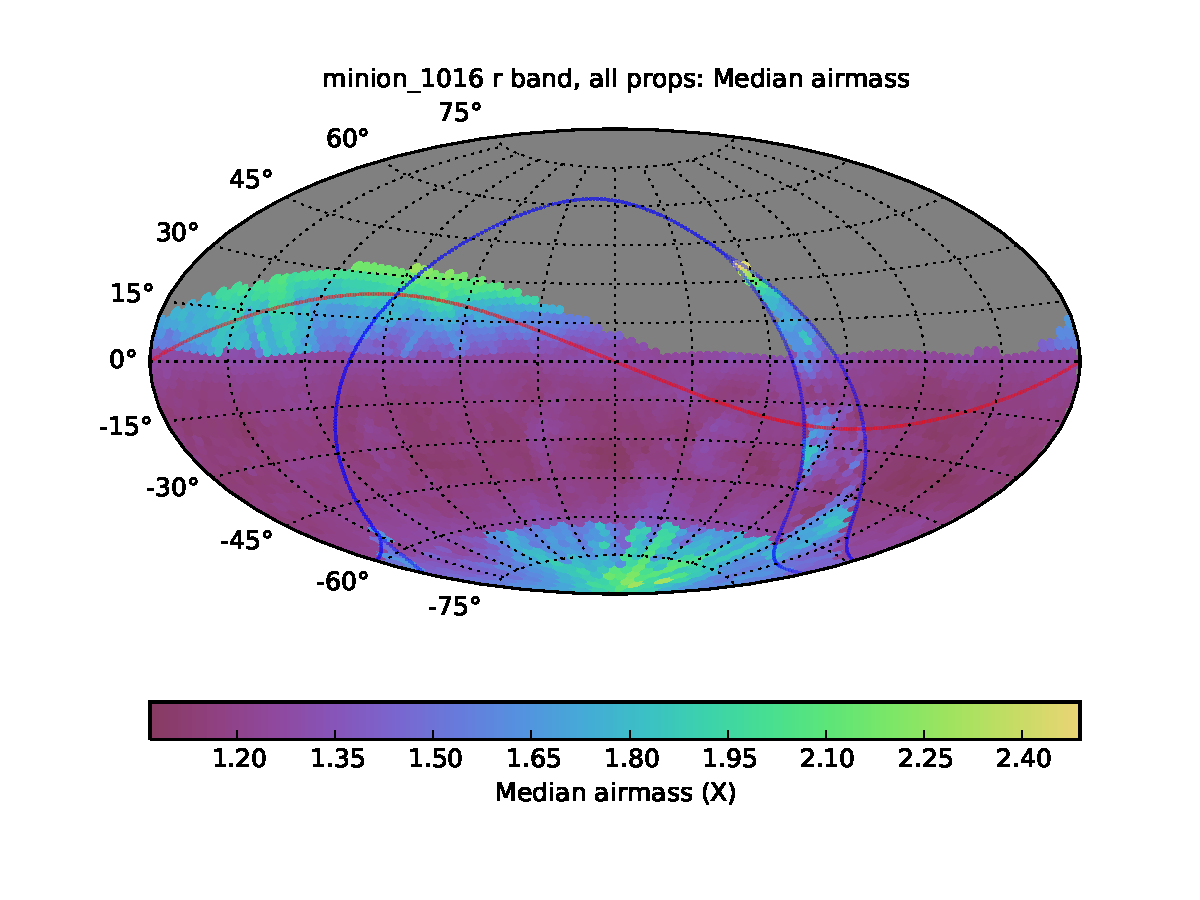
\includegraphics[angle=0,width=0.99\hsize,clip]{figs/cadence/minion_1016_Median_airmass_r_band_all_props_OPSI_SkyMap.pdf}
\end{subfigure}
\hfill
\begin{subfigure}[b]{0.49\textwidth}
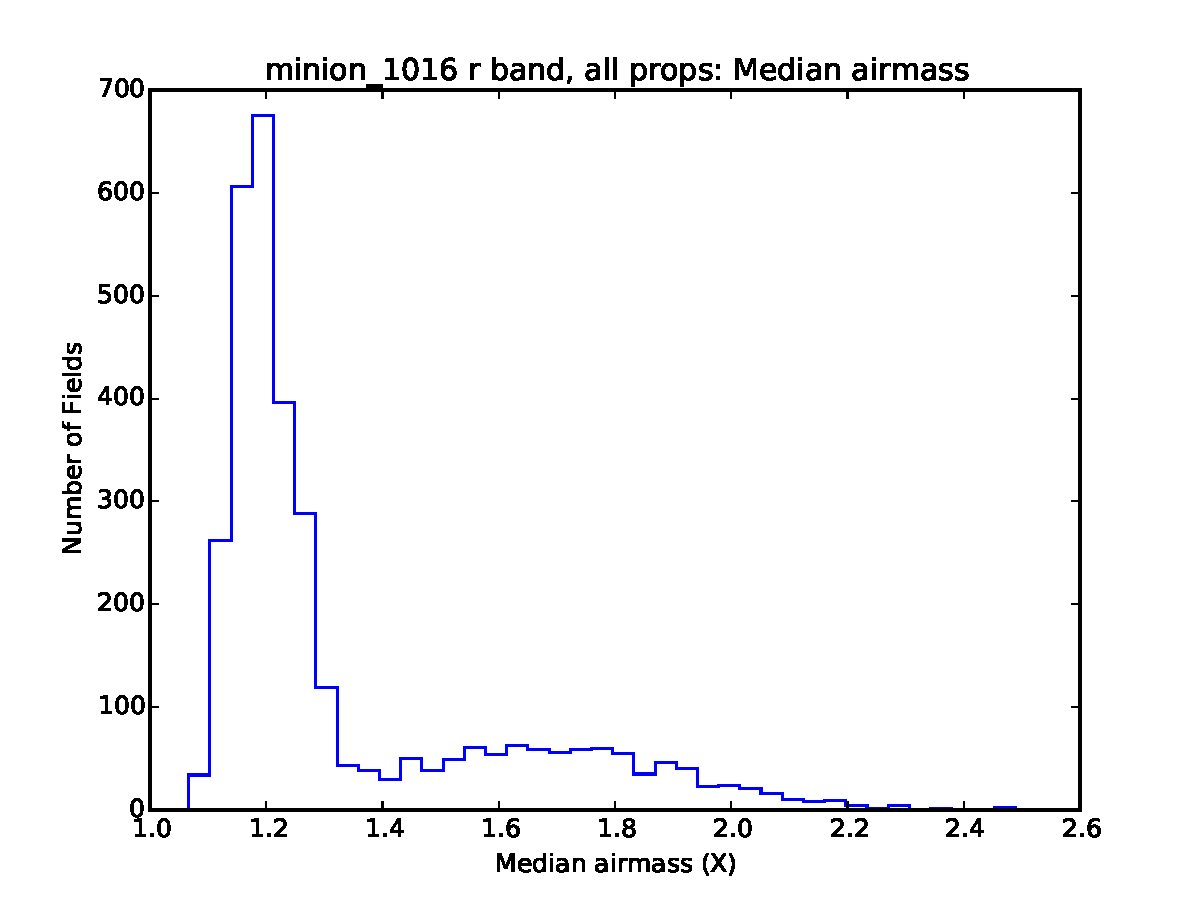
\includegraphics[angle=0,width=0.99\hsize,clip]{figs/cadence/minion_1016_Median_airmass_r_band_all_props_OPSI_Histogram.pdf}
\end{subfigure}
%\vskip -1.3in
\caption{The median airmass in the $r$ band across the sky for simulated cadence
\opsimdbref{db:baseCadence} is shown in Aitoff projection of equatorial coordinates 
in the left panel. The red line shows the Ecliptic and the blue line shows the Galactic 
equator (it bifurcates around the so-called ``Galactic confusion zone''). The corresponding 
airmass histogram is shown in the right panel. For the main survey area, the maximum 
allowed airmass was set to 1.5. }
\label{fig:airmassenigma}
\end{figure}
%%%%%%%%%%%%%%%%%%%%%%%%%%%%%%%%%
 
%%%%%%%%%%%%%%%%%%%%%%%%%%%%%%%%%
\begin{figure}[t!]
\vskip -0.1in
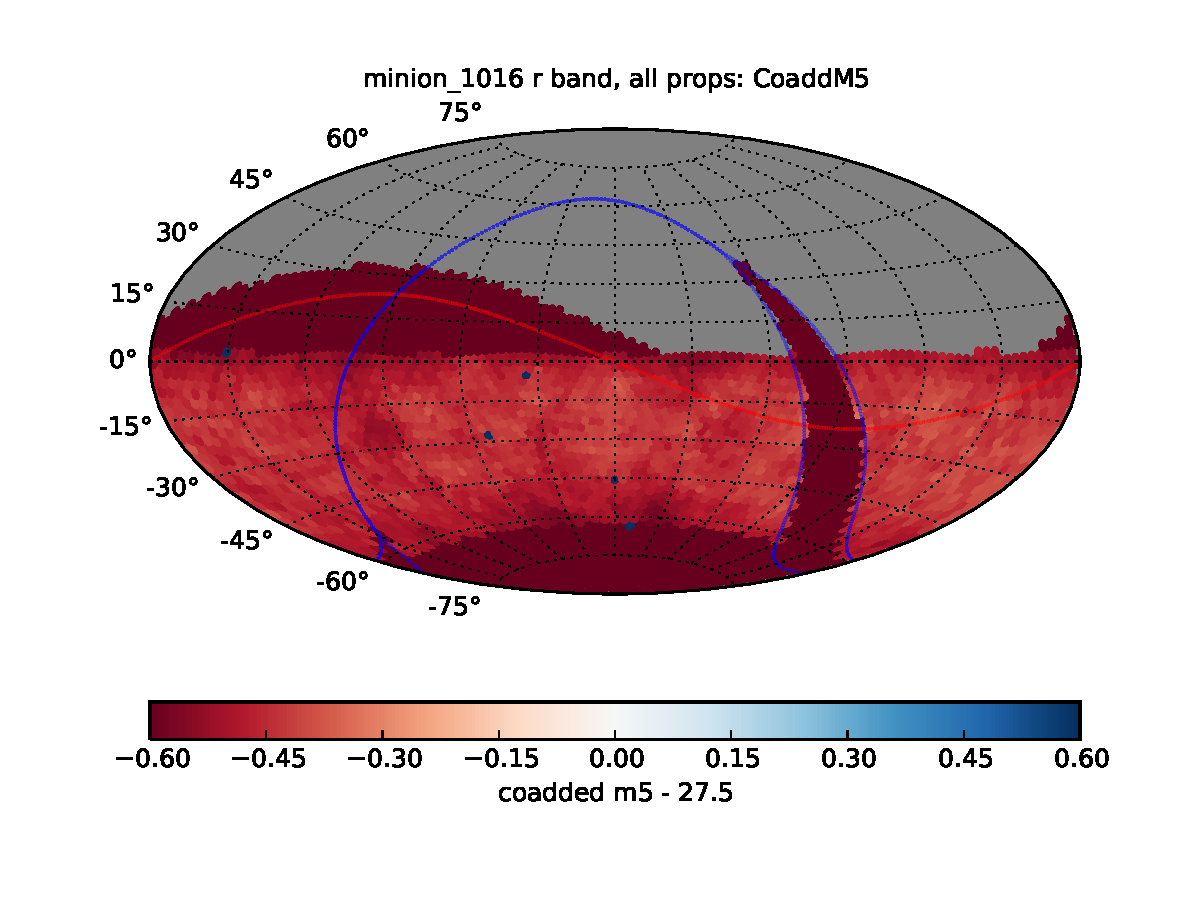
\includegraphics[angle=0,width=0.99\hsize,clip]{figs/cadence/minion_1016_CoaddM5_r_band_all_props_OPSI_SkyMap.pdf}
\vskip -0.5in
\caption{The coadded $5\sigma$ depth for point sources in the $r$ band 
across the sky for simulated cadence \opsimdbref{db:baseCadence} is shown 
in Aitoff projection of equatorial coordinates. The red line shows the Ecliptic and
the blue line shows the Galactic equator (it bifurcates around the so-called
``Galactic confusion zone''). The median value across the Universal Cadence area 
is 27.1, with RMS scatter of only 0.04 mag. The small dark dots are deep drilling 
fields, with a median $5\sigma$ depth of 28.6.}
\label{fig:coaddm5enigma}
\end{figure}
%%%%%%%%%%%%%%%%%%%%%%%%%%%%%%%%%

%%%%%%%%%%%%%%%%%%%%%%%%%%%%%%%%%
\begin{figure}[t!]
\vskip -0.0in
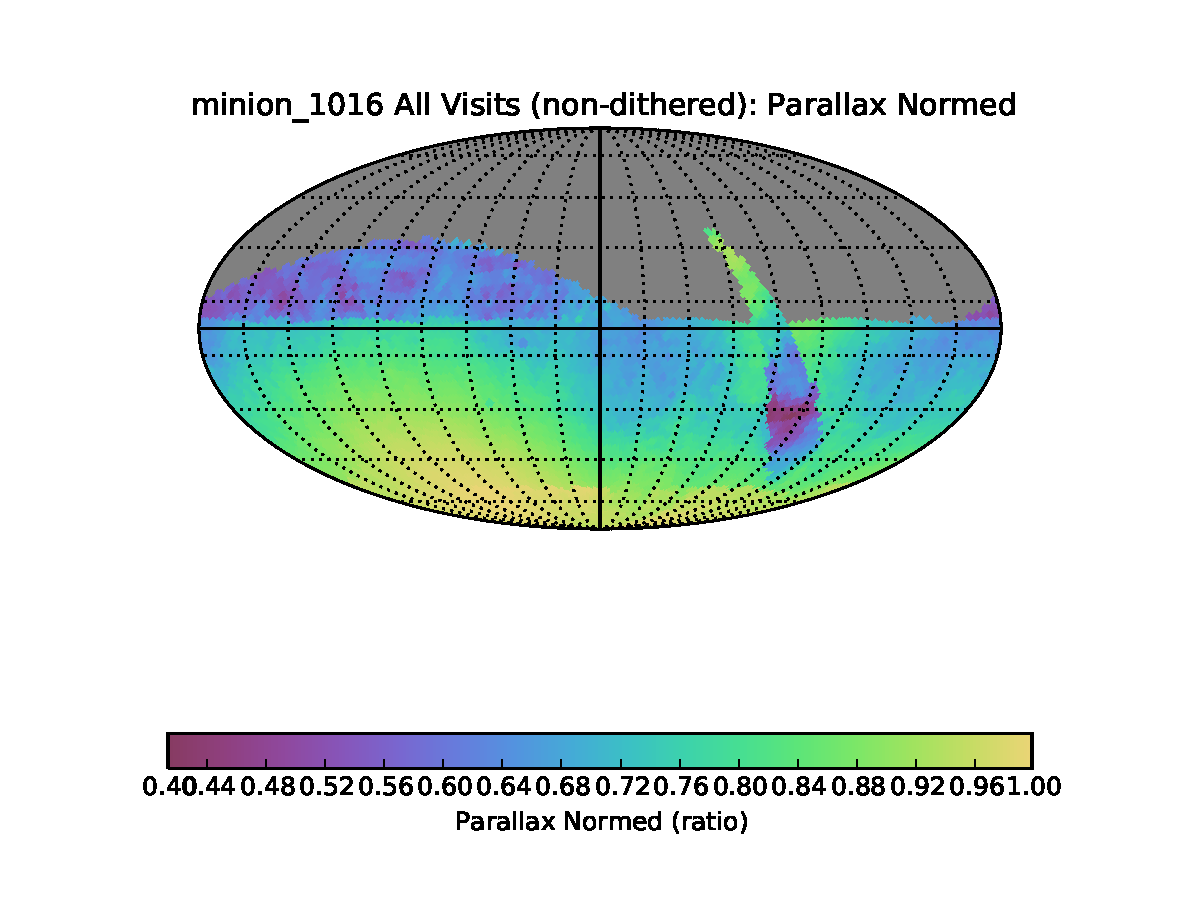
\includegraphics[angle=0,width=0.49\hsize,clip]{figs/cadence/minion_1016_Parallax_Normed_All_Visits_non-dithered_HEAL_SkyMap.pdf}
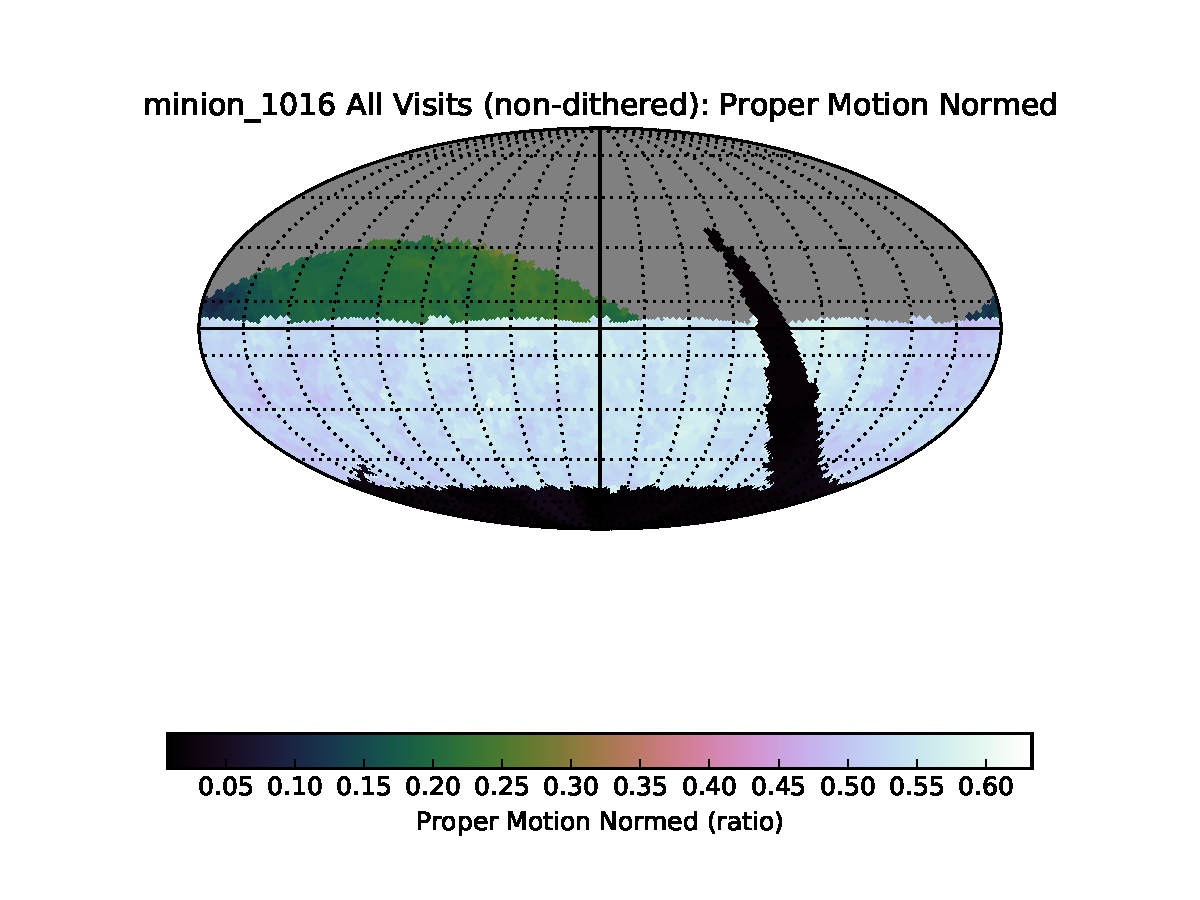
\includegraphics[angle=0,width=0.49\hsize,clip]{figs/cadence/minion_1016_Proper_Motion_Normed_All_Visits_non-dithered_HEAL_SkyMap.pdf}
\vskip -0.1in
\caption{The trigonometric parallax errors (left) and proper motion errors (right), normalized
by the values for idealized perfectly optimized cadences (parallax: all the observations are taken
at maximum parallax factor, resulting in a peak at the South Ecliptic pole; proper motion:
a half of all visits are obtained on the first day and the rest on the last day of the survey),
obtained for simulated cadence \opsimdbref{db:baseCadence} are shown in Aitoff projection of equatorial
coordinates.}
\label{fig:parapmenigma}
\end{figure}
%%%%%%%%%%%%%%%%%%%%%%%%%%%%%%%%%


The candidate replacement ``Baseline Cadence'' candidate,
\opsimdbref{db:baseCadence}, has the following basic
properties\footnote{For MAF output, see \url{http://ls.st/5ep}}:
\begin{enumerate}
\item The total number of visits is 2,447,931, with 85.1\% spent on
the Universal proposal (the main wide-fast-deep, WFD, survey), 6.5\% on the
North Ecliptic proposal, 1.7\% on the Galactic plane proposal, 2.2\%
on the South Celestial pole proposal, and 4.5\% on the Deep Drilling
cosmology proposal (5 fields).
\item The median number of visits {\it per night} is 816, the range is
88 to 1,104, with 3,026 observing nights. The mean slew time is 6.8
seconds (median: 4.8 sec) and the total exposure time is 7.34 Msec. 
The surveying efficiency, or the median total open shutter time (per night) 
as a fraction of the observing time (the ratio of the open shutter time and
the sum of the open shutter time, readout time and slew time) is 73\%. 
\item 
The 25\%-75\% quartiles for the number of filter changes per night are 2
and 6, with the mean of 4.3 The total number of filter changes is 14,194. 
\item In the $r$ band, the median effective seeing is 0.93 arcsec (for the more
traditional geometric FWHM, the median is 0.81 arcsec), the median
airmass is 1.23, and the median $5\sigma$ depth for point sources in WFD
area (also known as the Universal Cadence area) is 24.16 (using the best 
current estimate of the fiducial depth at airmass of one, $m_5(r)=24.39$, 
defined by the SRD Table 5). The variation of the median airmass for the $r$ 
band observations with the position on the sky is shown in
\autoref{fig:airmassenigma}.
\item The median single-visit depths for WFD fields are (23.14, 24.47, 24.16, 
23.40, 22.23, 21.57) in the $ugrizy$ bands\footnote{Note that these values
depend on externally supplied values for fiducial single-epoch
$5\sigma$ depths; the following values were used in analysis described
here: (23.62, 24.85, 24.39, 23.94, 23.36, 22.45) in the $ugrizy$
bands, respectively. These values are similar, but not identical, to the values
listed in Table 2 from the latest version (v3.1) of the LSST overview
paper: (23.68, 24.89, 24.43, 24.00, 23.45, 22.60). This discrepancy
is due to continuing improvements in the system performance estimates.}. 
These values are shallower than
the zenith dark time values for two main reasons: the sky is expected to be
brighter for non-dark time and away from zenith, the sky brightness model 
currently implemented in \OpSim has some shortcomings (a new model will
be implemented in version 4), and the moon avoidance is not as aggressive
as it could be. As a result, the limiting depths above are biased bright by close
to 1 mag in the $z$ and $y$ bands, and a few tenths of a magnitude in the 
$u$, $g$ and $i$ bands. The co-added depths are tied to single-visit bands,
and suffer from the same bias. 
\item For the 2,293 (overlapping) fields from the WFD area, 
the median number of visits in the $ugrizy$ bands is (62, 88, 199, 201, 180,
180), respectively. Not only do these medians exceed the requested
number of visits (design specification from the SRD\footnote{The LSST
Science Requirements Document (SRD) is available as
\url{http://ls.st/lpm-17}}) of (56, 80, 184, 184, 160, 160) in the $ugrizy$
bands, but the minimum number of visits per field over this area does
so, too. This result is quite encouraging given that 
only 85\% of observing time was spent on the Universal Cadence proposal. 
\item The median coadded $5\sigma$ depth 
for point sources in the $ugrizy$ bands is (25.4, 27.0, 27.1, 26.4,
25.2, 24.4), respectively, for the Universal Cadence area. The distribution 
of coadded depth across the sky is fairly uniform, as illustrated in \autoref{fig:coaddm5enigma}.
\item For the 2,293 fields from the Universal Cadence area, the median
geometric FWHM for seeing is 0.78 arcsec in the $r$ band and 0.77 arcsec 
in the $i$ band. The median airmass in the $urz$ bands is 1.25, 1.20 and 1.26 
(the maximum allowed airmass for the Universal Cadence area was set to
1.5).  The median sky brightness in the $ury$ bands is 22.0 mag/arcsec$^2$, 
21.1 mag/arcsec$^2$, and 17.3 mag/arcsec$^2$, respectively (for comparison,
assumed dark sky brightness in the $ury$ bands is 23.0, 21.2 and 18.6 
mag/arcsec$^2$).  The current model sky brightness in the $y$ band is biased 
high by close to 1 mag. 
\item Restricted to the Universal Cadence fields, a unique area of
18,000 sq.deg. received at least 888 visits per field (summed over bands; 
the SRD design value is 825).
\item The median trigonometric parallax and proper motion errors are
0.62 mas and 0.17 mas/yr, respectively, for bright sources (limited by
assumed systematic errors in relative astrometry of 10 mas), and 7.9
mas and 2.3 mas/yr for points sources with $r=24$ (assuming flat
spectral energy distribution), over the Universal Cadence fields. The
variation of parallax and proper motion errors across the sky is
visualized in \autoref{fig:parapmenigma}.
\end{enumerate}





For comparison, the current Baseline Cadence, \texttt{opsim3.61}
(obtained with old OpSim code), delivered 2,651,588 visits, or 8.3\%
more than \opsimdbref{db:baseCadence}  (this is due to known effects and
changes in the code,  such as more pre-scheduled down time in the new
version). Perhaps the most important (and undesired!) difference
between the two simulations is that the new candidate Baseline Cadence
spent 6.5\% of the observing time on North Ecliptic Spur proposal (vs.
4\% spent on the corresponding Universal North proposal in
\texttt{opsim3.61}), and less than 90\% of time on the Universal
proposal (the main wide-deep-fast survey).

Analysis of the hour angle distribution, shown in
\autoref{fig:HAenigma} and \autoref{fig:AltAzenigma}, reveals a strong
bias towards observations west from the meridian for the main survey.
{\it This pattern is not fully understood at this time} and may be
caused by specific features of the cost function implemented in the
OpSim code.



%%%%%%%%%%%%%%%%%%%%%%%%%%%%%%%%%
\begin{figure}[t!]
\vskip -0.0in
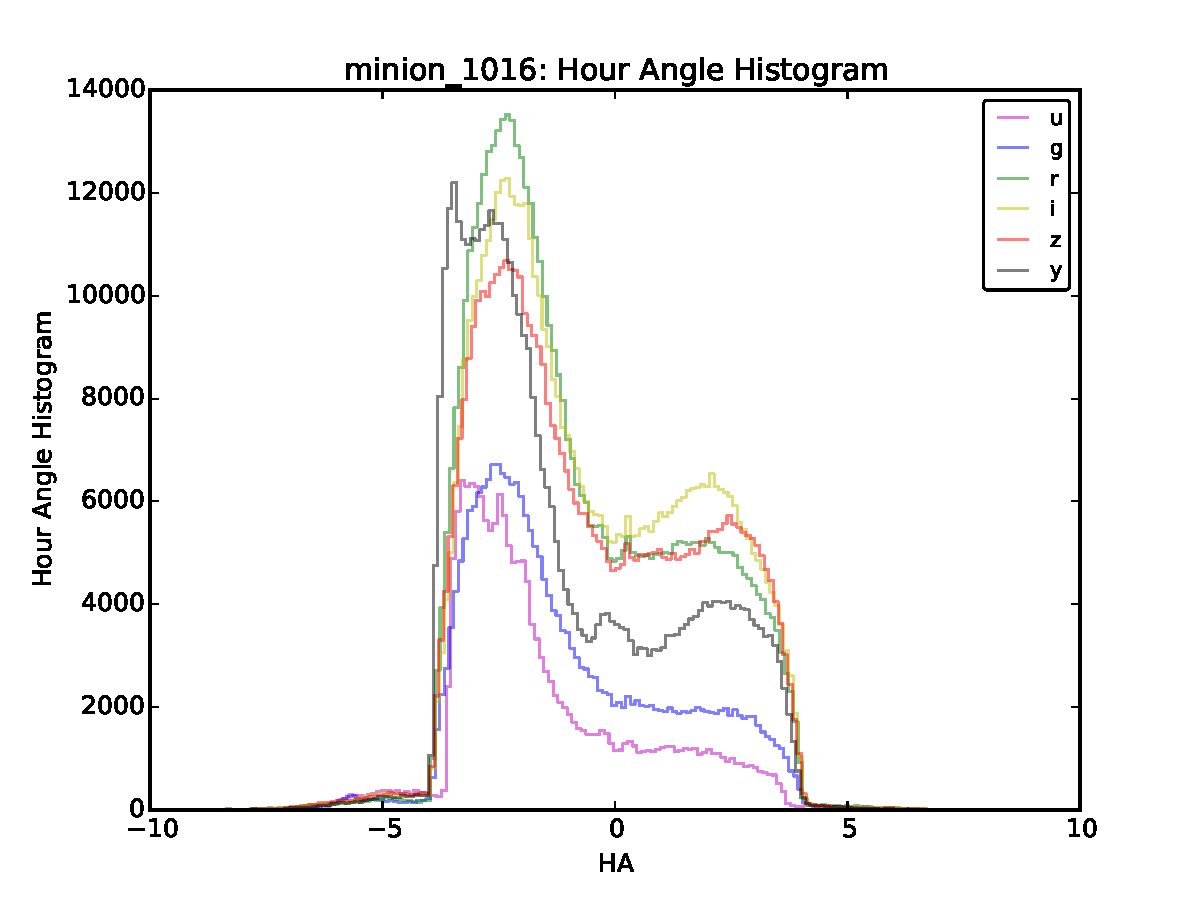
\includegraphics[angle=0,width=0.49\hsize,clip]{figs/cadence/minion_1016_Hour_Angle_Histogram_u_g_r_i_z_y_band_all_props_ONED_ComboBinnedData.pdf}
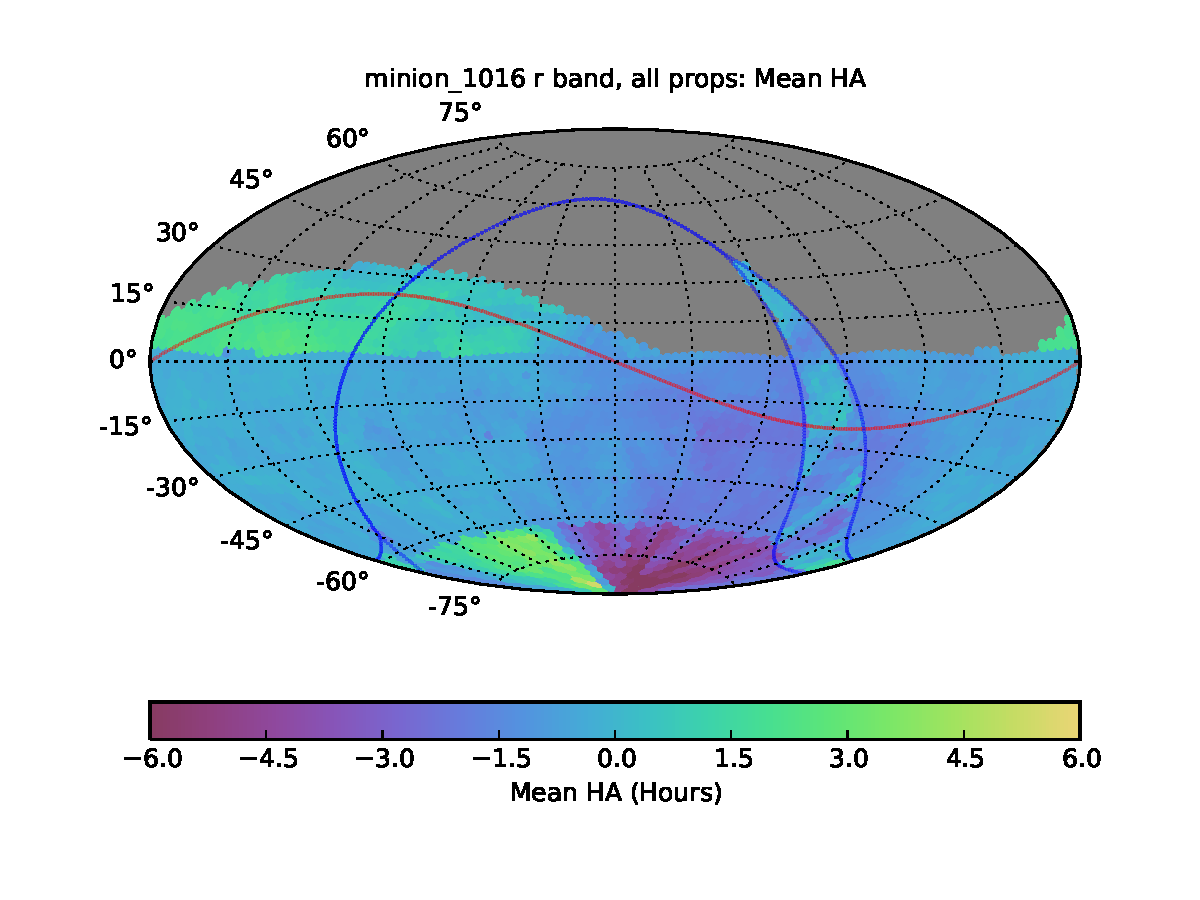
\includegraphics[angle=0,width=0.49\hsize,clip]{figs/cadence/minion_1016_Mean_HA_r_band_all_props_OPSI_SkyMap.pdf}
\vskip -0.1in
\caption{Histograms in the left panel show the distribution of hour angles (HA) in
6 bands for all proposals from simulated cadence \opsimdbref{db:baseCadence} (the distributions are
similar for WFD fields considered alone). Note the bias towards observations west from
the meridian. The right panel shows the distribution across the sky of the mean HA for
all observations in the $r$ band. }
\label{fig:HAenigma}
\end{figure}
%%%%%%%%%%%%%%%%%%%%%%%%%%%%%%%%%

%%%%%%%%%%%%%%%%%%%%%%%%%%%%%%%%%
\begin{figure}[t!]
\vskip -0.0in
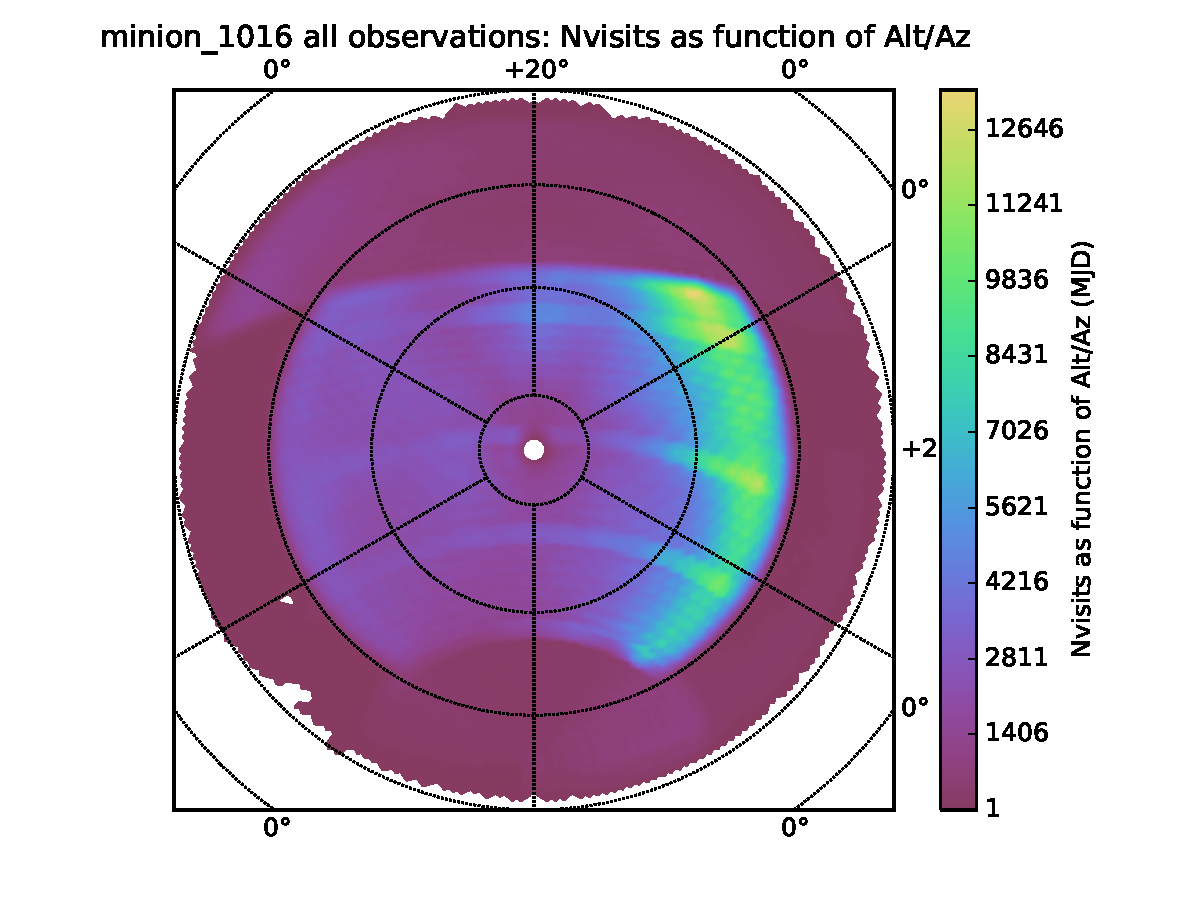
\includegraphics[angle=0,width=0.49\hsize,clip]{figs/cadence/minion_1016_Nvisits_as_function_of_Alt_Az_all_observations_HEAL_SkyMap.pdf}
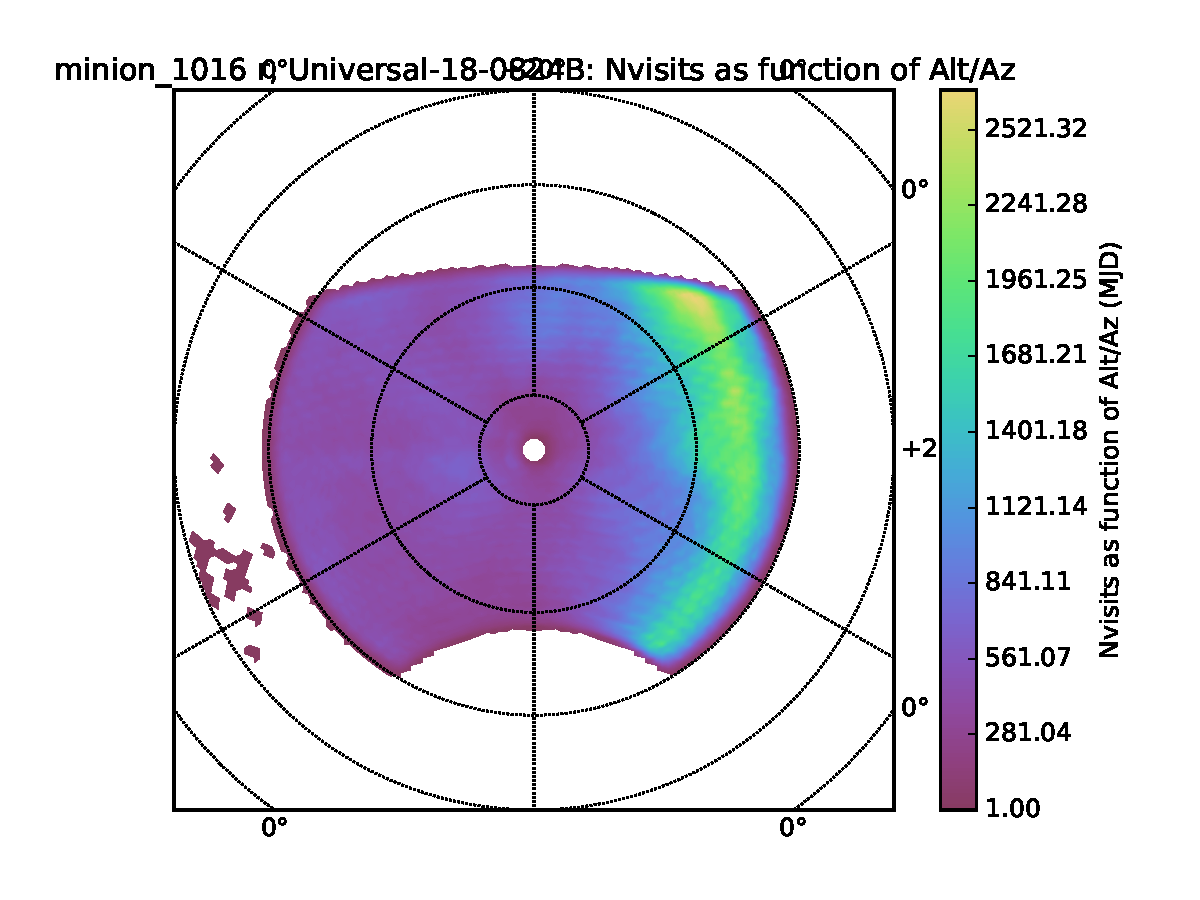
\includegraphics[angle=0,width=0.49\hsize,clip]{figs/cadence/minion_1016_Nvisits_as_function_of_Alt_Az_r_Universal-18-0824B_HEAL_SkyMap.pdf}
\vskip -0.1in
\caption{The color-coded map in the left panel shows the visit count from
Baseline Cadence simulation \opsimdbref{db:baseCadence} in the equal-area Lambert projection of the
horizontal coordinate system (altitude-azimuth), with north on top and west towards the
right, for all six bands and proposals (Universal, Galactic Plane, Deep Drilling
fields, North Ecliptic Spur, and South Celestial Pole region). The Universal cadence was
limited to airmass below 1.5, while other proposals sampled higher airmass, too (see the
histogram in \autoref{fig:airmassenigma}).  Note the strong propensity of fields
for westward observations (the median airmass is about 1.2). The right panel is analogous,
but only shows the $r$ band visits for WFD fields.}
\label{fig:AltAzenigma}
\end{figure}
%%%%%%%%%%%%%%%%%%%%%%%%%%%%%%%%%







%%%%%%%%%%%%%%%%%%%%%%%%%%%%%%%%%
\begin{figure}[th!]
\vskip -0.0in
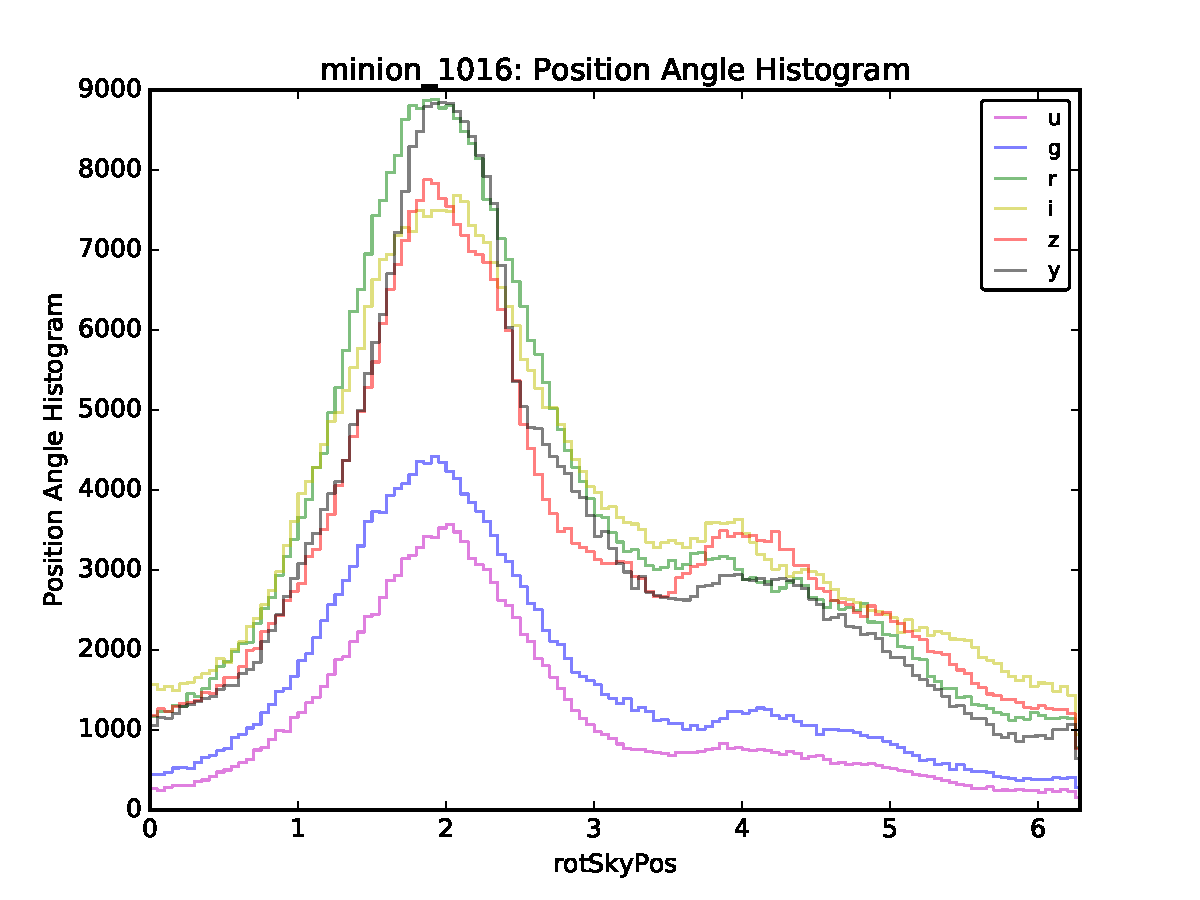
\includegraphics[angle=0,width=0.49\hsize,clip]{figs/cadence/minion_1016_Position_Angle_Histogram_u_g_r_i_z_y_band_WFD_ONED_ComboBinnedData.pdf}
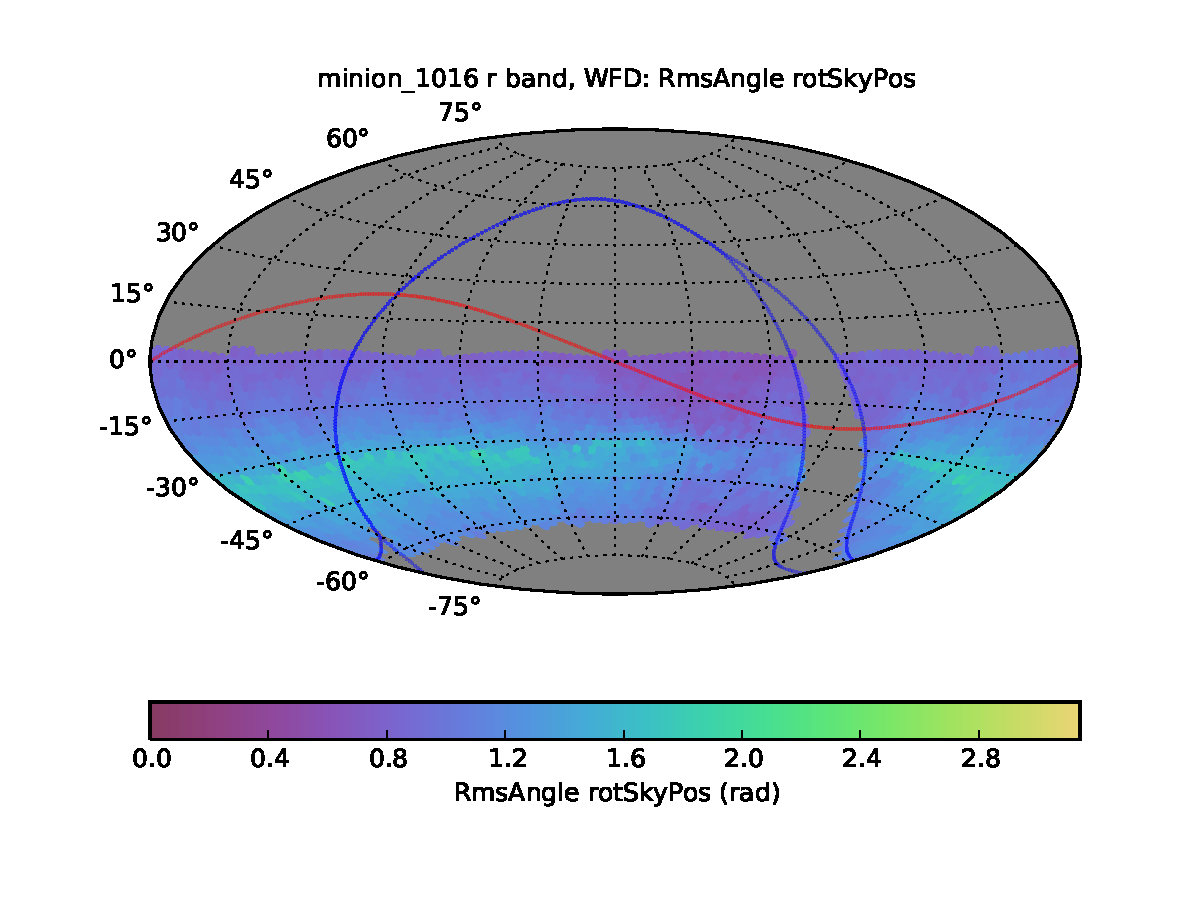
\includegraphics[angle=0,width=0.49\hsize,clip]{figs/cadence/minion_1016_RmsAngle_rotSkyPos_r_band_WFD_OPSI_SkyMap.pdf}
\vskip -0.1in
\caption{The left panel shows the position angle distribution (in radians)  in each band for the
main survey fields in \opsimdbref{db:baseCadence}. The position angle is the angle between 
``up'' in the image and North on the sky. The variation of the root-mean-square scatter of the 
$r$ band distribution across the sky is shown in the right panel.}
\label{fig:rotator}
\end{figure}
%%%%%%%%%%%%%%%%%%%%%%%%%%%%%%%%%

Another potentially undesirable feature, seen in practically all
simulations analyzed here, is that up to about a quarter of visits in
the main survey area represents the third, the fourth and sometimes
even the fifth visit to a field in the same night. For a large number
of time-domain programs, these visits could be used instead to
decrease the field inter-night revisit time. For more details, see
\autoref{sec:cadexp:NEOs}. The position angle distributions for this simulation
are shown in \autoref{fig:rotator}.


\subsubsection{Time-domain metrics}

The analysis of metrics designed for time-domain science has not been
performed yet in detail, except for the analysis of asteroid
completeness discussed in \autoref{sec:cadexp:NEOs}. MAF already includes
several sophisticated metrics, e.g., period recovery for variable
stars, which will be described in a later version of this report.

As a brief illustration of time-domain analysis,
\autoref{fig:enigmaGapAll} shows the median revisit time distribution
when all bands are considered, and \autoref{fig:enigmaGapr} shows the
median revisit time distribution in the band.  On average, fields in
the main survey get revisited about every 3 days using all filters,
and every 15 days when using only r band visits (30 days when using
only u band visits is the longest median revisit time).
\autoref{fig:enigmaMAXGapAll} shows the maximum inter-night gap, which
on average is about 5-6 months.

The temporal sampling for this simulation is sufficient to enable a
large recovery fraction for SNe. \autoref{fig:enigmaEarlySNe} shows
that a large fraction of LSST SNe will be detected before their
maximum brightness. Similar MAF metrics that explore various quality
cuts on SNe light curves (e.g. ``detected at least 6 times, at least 3
pre-peak, at least 3 post-peak, with observations in at least 3
filters'').

Intra-night revisit time distribution is discussed in more detail in
\S\ref{sec:cadexp:NEOs}.


%%%%%%%%%%%%%%%%%%%%%%%%%%%%%%%%%
\begin{figure}[t!]
\vskip -0.0in
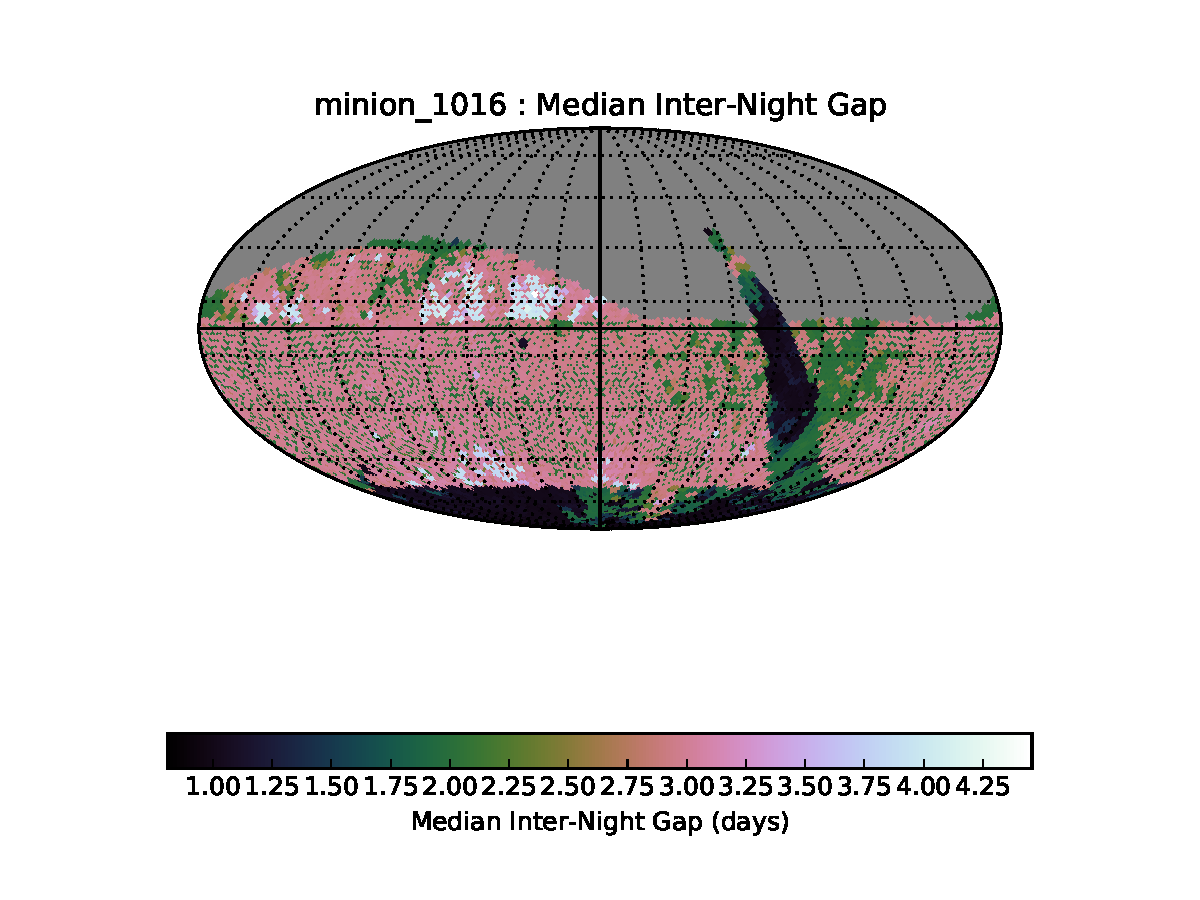
\includegraphics[angle=0,width=0.49\hsize,clip]{figs/cadence/minion_1016_Median_Inter-Night_Gap_HEAL_SkyMap.pdf}
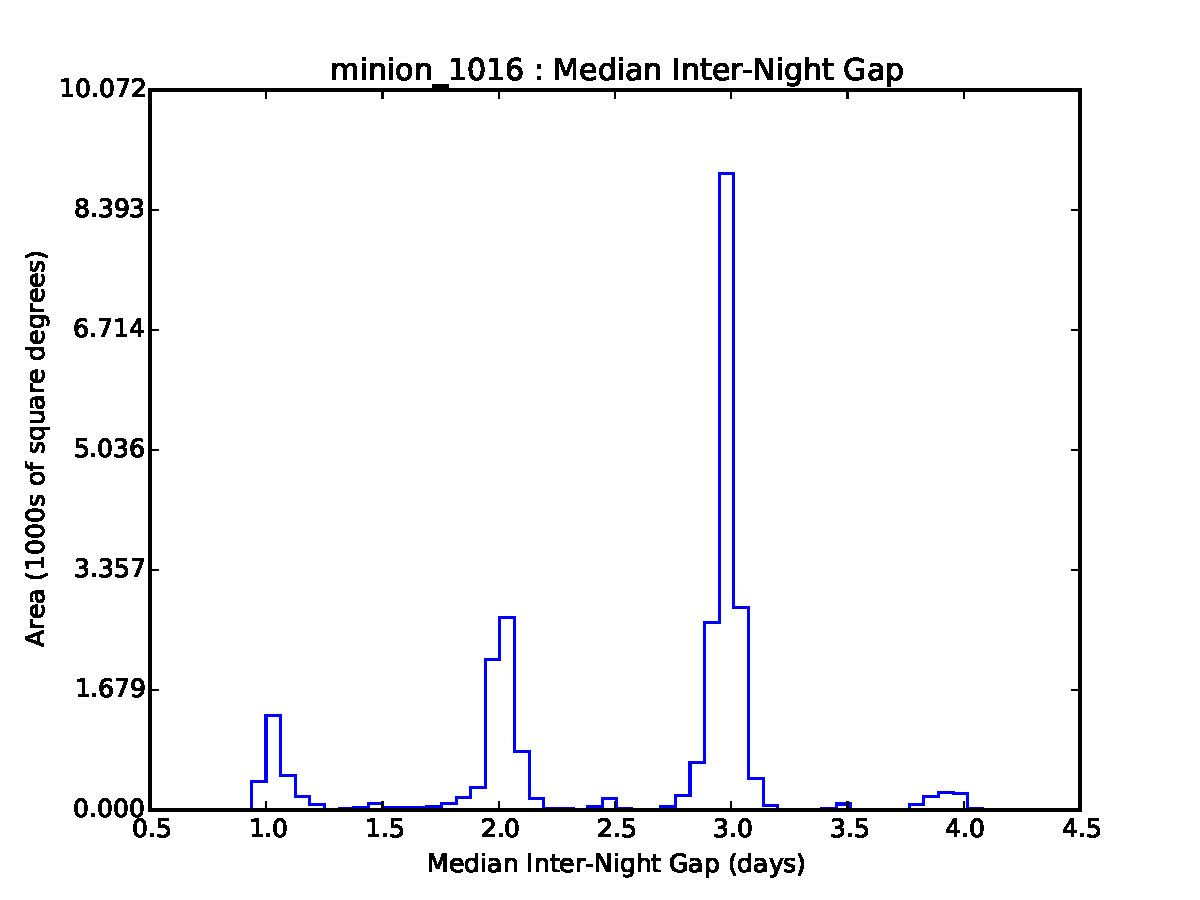
\includegraphics[angle=0,width=0.49\hsize,clip]{figs/cadence/minion_1016_Median_Inter-Night_Gap_HEAL_Histogram.pdf}
\vskip -0.1in
\caption{The median inter-night gap (or revisit time) is shown in Aitoff projection
for all proposals and all filters for candidate Baseline Cadence \opsimdbref{db:baseCadence}.
On average, fields in the main survey get revisited about every 3 days.}
\label{fig:enigmaGapAll}
\end{figure}
%%%%%%%%%%%%%%%%%%%%%%%%%%%%%%%%%

%%%%%%%%%%%%%%%%%%%%%%%%%%%%%%%%%
\begin{figure}[h!]
\vskip -0.0in
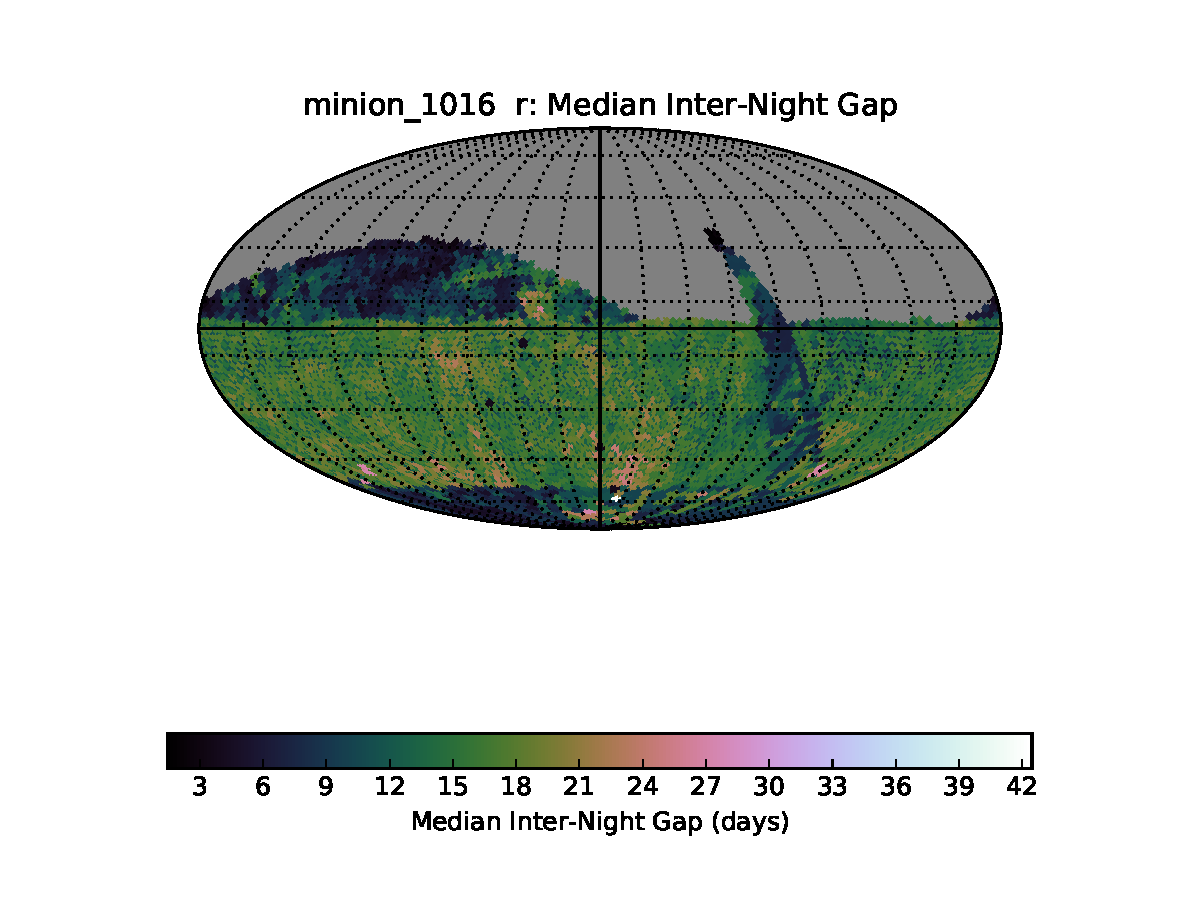
\includegraphics[angle=0,width=0.49\hsize,clip]{figs/cadence/minion_1016_Median_Inter-Night_Gap_r_HEAL_SkyMap.pdf}
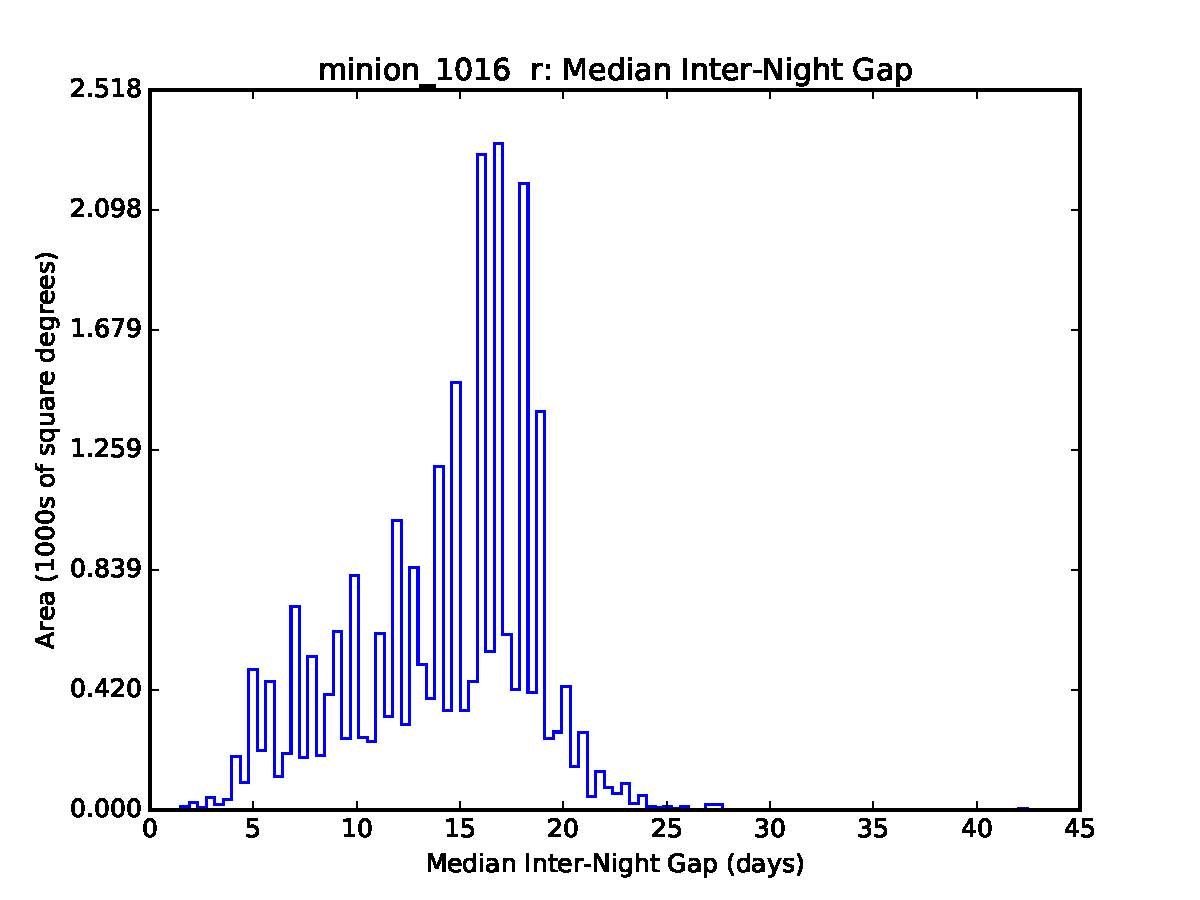
\includegraphics[angle=0,width=0.49\hsize,clip]{figs/cadence/minion_1016_Median_Inter-Night_Gap_r_HEAL_Histogram.pdf}
\vskip -0.1in
\caption{The median inter-night gap for r band visits is shown in Aitoff projection
for all proposals and all filters for candidate Baseline Cadence \opsimdbref{db:baseCadence}.
On average, fields in the main survey get revisited in the r band about every two weeks.}
\label{fig:enigmaGapr}
\end{figure}
%%%%%%%%%%%%%%%%%%%%%%%%%%%%%%%%%

%%%%%%%%%%%%%%%%%%%%%%%%%%%%%%%%%
\begin{figure}[t!]
\vskip -0.0in
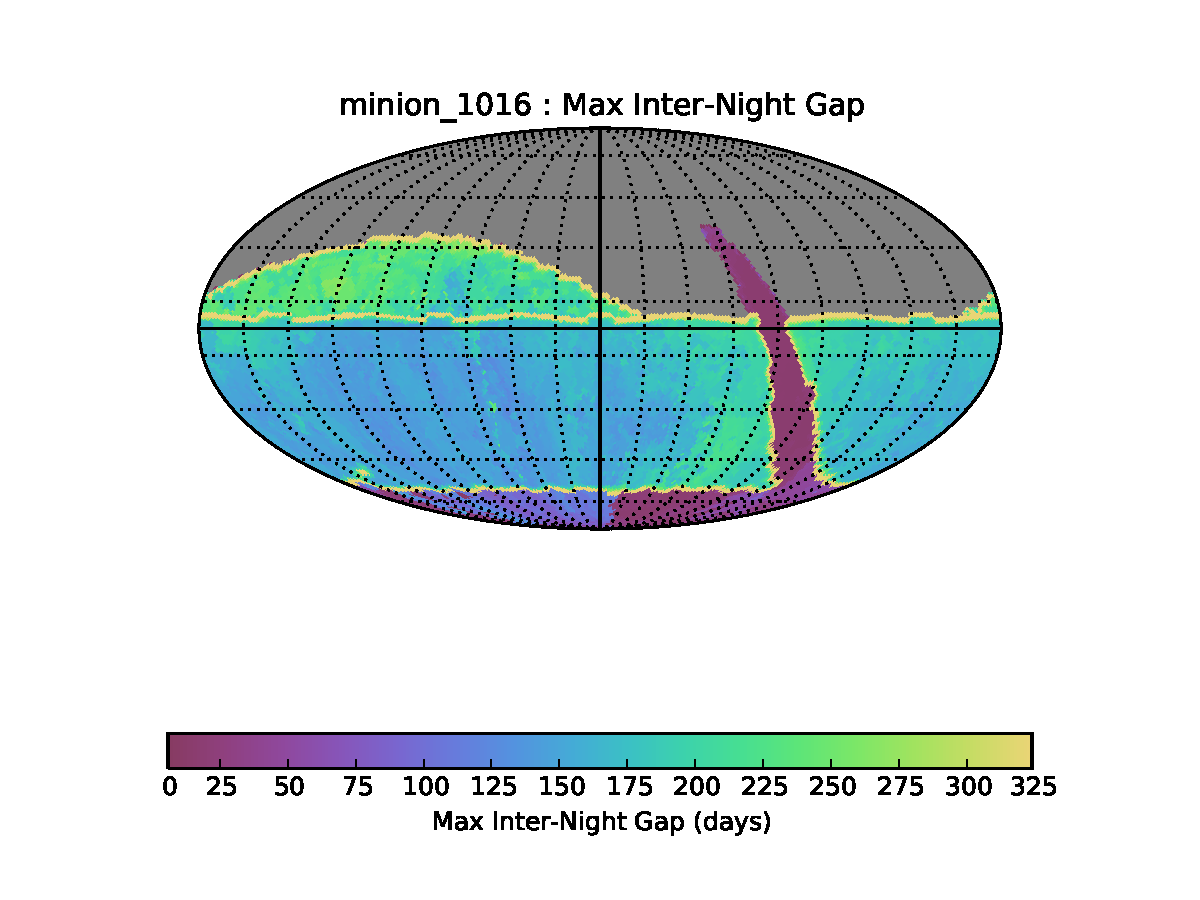
\includegraphics[angle=0,width=0.49\hsize,clip]{figs/cadence/minion_1016_Max_Inter-Night_Gap_HEAL_SkyMap.pdf}
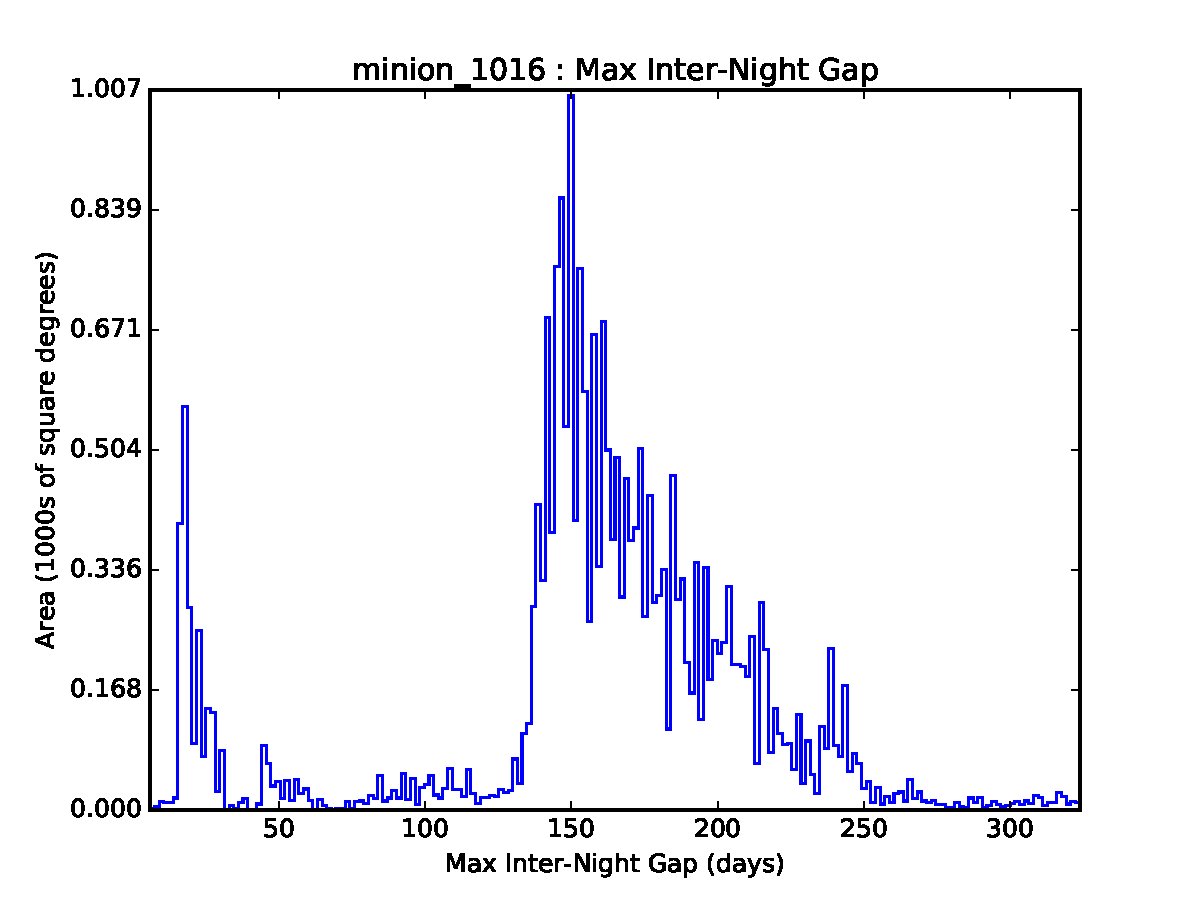
\includegraphics[angle=0,width=0.49\hsize,clip]{figs/cadence/minion_1016_Max_Inter-Night_Gap_HEAL_Histogram.pdf}
\vskip -0.1in
\caption{The maximum inter-night gap (or revisit time) is shown in Aitoff projection
for all proposals and all filters for candidate Baseline Cadence \opsimdbref{db:baseCadence}.}
\label{fig:enigmaMAXGapAll}
\end{figure}
%%%%%%%%%%%%%%%%%%%%%%%%%%%%%%%%%



%%%%%%%%%%%%%%%%%%%%%%%%%%%%%%%%%
\begin{figure}[h!]
\vskip -0.0in
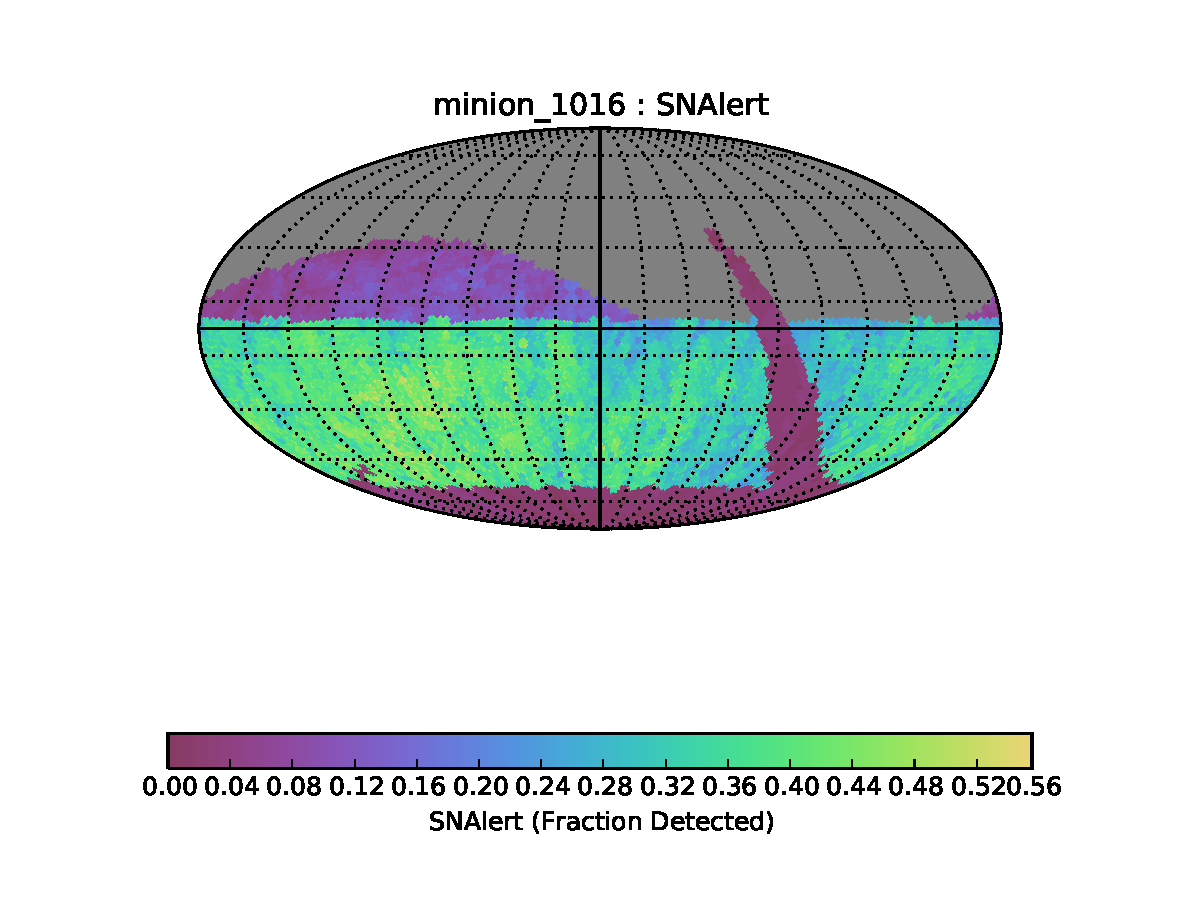
\includegraphics[angle=0,width=0.49\hsize,clip]{figs/cadence/minion_1016_SNAlert_HEAL_SkyMap.pdf}
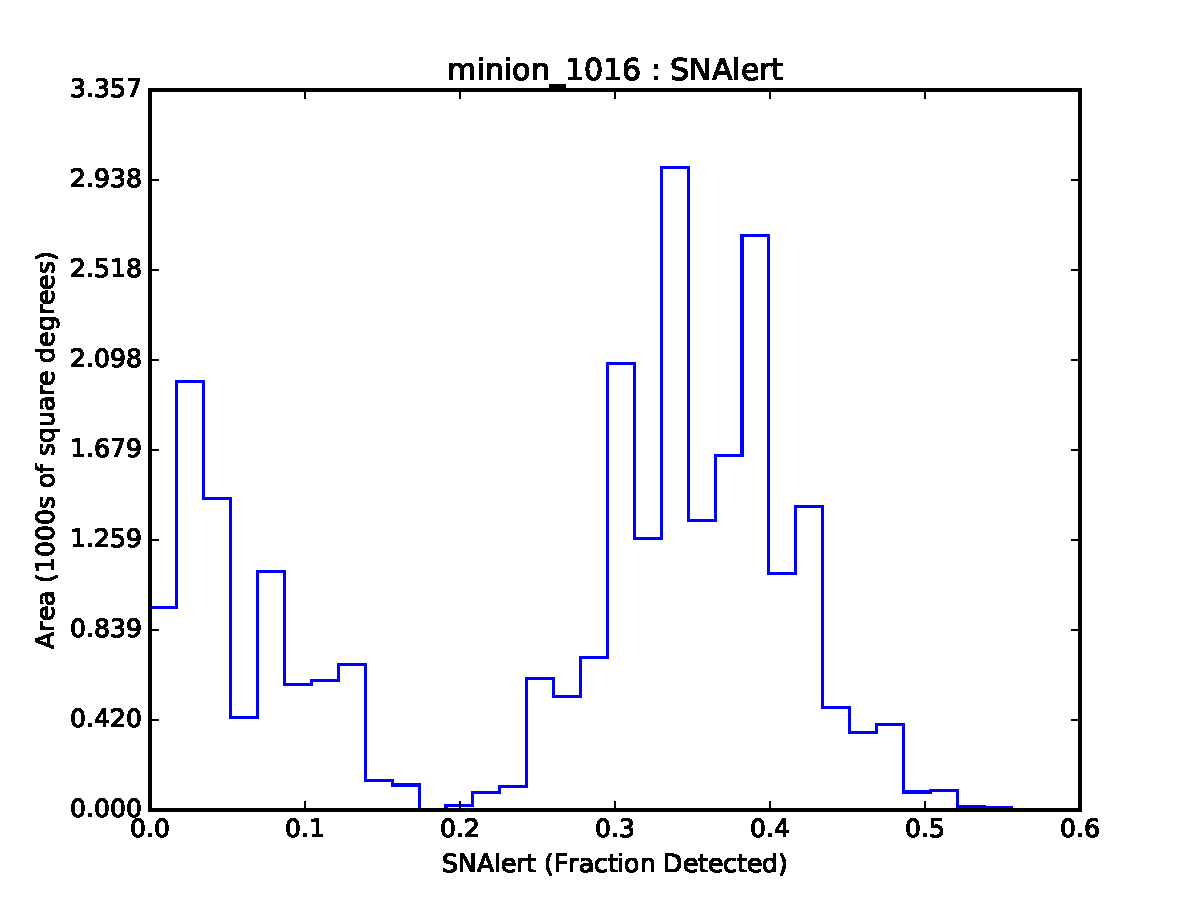
\includegraphics[angle=0,width=0.49\hsize,clip]{figs/cadence/minion_1016_SNAlert_HEAL_Histogram.pdf}
\vskip -0.1in

\caption{The fraction of simulated Type Ia SNe at a redshift of 0.5 detected
pre-peak in any filter for candidate Baseline Cadence \opsimdbref{db:baseCadence}. About
40\% of all such SNe from the main survey will be detected before their
maximum brightness.}
\label{fig:enigmaEarlySNe}
\end{figure}
%%%%%%%%%%%%%%%%%%%%%%%%%%%%%%%%%



\subsubsection{Special Proposals}

Regarding the special proposals, here we only provide the basic
performance parameters. With the exception of the Deep Drilling
proposal, these proposals are essentially strawman placeholders. The
North Ecliptic proposal (6.4\% of the observing time) obtained an
additional 300 visits per field, summed over $griz$ bands. These
fields are placed along the northern part of the Ecliptic. The
Galactic plane proposal (1.7\%) obtained 30 visits per band in all six
bands, across the region extending in Galactic latitude 10 degrees
from the Galactic center, with the boundary approaching the Galactic
equator linearly with longitude, and the zone ending at $l=90$ deg.
and at $l=270$ deg. The South Celestial pole proposal (2.1\%) obtained
30 visits per band in all six bands, for fields centers with Dec $<
-62.5$ deg. The Deep Drilling cosmology proposal (4.5\%) included 5
fields, with each obtaining several thousand visits per band. The
coadded $5\sigma$ depths for these fields are much fainter than for
the main survey: the median values are (27.8, 28.4, 28.6, 28.0, 27.6,
26.1) in the $ugrizy$ bands, respectively.


\vskip 0.2in
{\bf Conclusions:}

The candidate “Baseline Cadence”, \opsimdbref{db:baseCadence}, appears to
be an adequate replacement for the current baseline cadence
(\texttt{opsim3.61}). Based on this preliminary analysis, there are no
major problems with its performance. While there are patterns which
are not fully understood (most notably the observing bias towards
west),  or undesired (unnecessary revisits of the same field in the
same night), \opsimdbref{db:baseCadence} is used as a benchmark cadence,
and referred to as ``Baseline Cadence'',  in the rest of this
document\footnote{This simulation was proposed by the Project Science Team 
for adoption as the new Baseline Cadence to the Change Control Board.}

An important feature of \opsimdbref{db:baseCadence} simulation is that
the mean slew time of 6.8 sec (which includes filter change time) is
very close to the minimum possible slew time of about 4.5 sec. The
implication is that the surveying efficiency, assuming 30 sec exposure
time per visit, can be increased by at most about 6\% (that is, the
total open-shutter time is within about 6\% from its possible maximum,
given everything else unchanged).  Nevertheless, there are other
survey aspects, including sky coverage and temporal sampling
functions, that can be further optimized, as discussed in
\autoref{sec:cadexp:alternatives} below.

{\bf The main remaining known problems} with \opsimdbref{db:baseCadence} simulation include
\begin{itemize}
\item A strong bias towards observations west from the meridian for
  the main survey, see \autoref{fig:AltAzenigma}.  This bias
  significantly degrades the survey seeing and depth.
\item Several proposals complete after only 3-4 years, resulting in
  regions of sky where the proper motions are poorly constrained due
  to the short observing baseline.  See \autoref{fig:parapmenigma2}.
\item The sky brightness model has systematic errors in red bands,
  resulting in estimates of limit depths ($m_5$, both for single
  visits and coadded depths) that are too shallow by about 0.3 mag in
  the $u$ band, and 0.5 mag in the $z$ and $y$ bands.
\item The moon avoidance angle of 30 deg. allows too many $z$ band
  observations with elevated sky brightness due to moonshine,
  resulting in about 0.2-0.3 mag shallower depth.
\item There are too many unrequested and unnecessary revisits of the
  same field in the same night (that is, more than two visits to the
  same field in the same night).
\end{itemize}

\navigationbar
% --------------------------------------------------------------------








% --------------------------------------------------------------------

\section{Some Simulated Alternative Observing Strategies}
\def\secname{cadexp:alternatives}\label{sec:\secname}

We now describe some alternatives to the Baseline Cadence that were
explored. These \OpSim databases are all available for further testing
with science-based MAF metrics.

% - - - - - - - - - - - - - - - - - - - - - - - - - - - - - - - - - -

%%%%%%%%%%%%%%%%%%%%%%%%%%%%%%%
\opsimdb[db:opstwo]{minion\_1012}{Only Universal Cadence, with pairs of visits.}
%%%%%%%%%%%%%%%%%%%%%%%%%%%%%%%

{\bf Motivation and description:} Formally, $\sim$90\% of observing
time is allocated to the main Universal Cadence program (WFD). The
remaining observing time is allocated to other programs, such as
``Deep Drilling'' programs (see Section 3.4 and Tables 22-26  in the
SRD). With this simulation, we wished to find out what would be the
effect of ignoring special programs and spending all of the observing
time on the main Universal Cadence program. \\

{\bf Expectations:} About 2.08 million visits (85\% of 2.44 million
visits) from Baseline Cadence (\opsimdbref{db:baseCadence}) were allocated
to WFD cadence. Here we expect that all of these 2.44 million visits
will be allocated to WFD cadence. \\

{\bf Analysis Results:} This simulated cadence is named \opsimdbref{db:opstwo}.
Compared to the Baseline Cadence \opsimdbref{db:baseCadence}:
\begin{enumerate}
\item The total number of visits is close to the expected value: 2.42 million.
The minimum number of visits per field for the 2,293 WFD fields in Baseline Cadence
is 966 for this simulation, compared to 888 for Baseline Cadence.
\item The median number of visits per night and the mean slew time are
essentially the same as for Baseline Cadence (807 vs. 816 and 7.2 sec vs. 6.8 sec).
\item The median seeing, sky brightness and airmass in the r and i bands are
      essentially the same as for WFD fields in Baseline Cadence.
\item XXX The median trigonometric parallax and proper motion errors are improved by
about 8\%, with improvements commensurate with the increase in the number of visits.
\item This simulation also shows observing bias towards west (that is, additional
special programs in \opsimdbref{db:baseCadence} are not responsible for this bias).
\end{enumerate}


{\bf Conclusions:} \opsimdbref{db:opstwo}, using only uniform cadence
proposal, delivered 99.2\% of the number of visits obtained by
Baseline Cadence. Therefore, {\it the ``filler'' aspect of other
proposals does not have a major impact on the surveying efficiency}.
The minimum number of visits per field for the 2,293 WFD fields in
Baseline Cadence is 968 (the SRD design value is 825 and the stretch
goal value is 1000). Although the sky coverage of these 2293 fields is
about 18,000 sq.deg., their cumulative area is 22,000 sq.deg. With
proper dithering, the effective number of visits could be increased to
$968\times22/18 = 1183$ (or the WFD area increased from 18,000 sq. deg.; see
analysis of ops2\_1092 below). This increase is an improvement of 43\%
relative to the SRD design specification of 825 visits over 18,000
sq.deg. However, note again that there are no other programs in this
simulation (i.e., if other programs were allocated 10\% of the
observing time, the implied overall ``over-performance'' in the number
of  visits would be about 30\%).

% - - - - - - - - - - - - - - - - - - - - - - - - - - - - - - - - - -

%%%%%%%%%%%%%%%%%%%%%%%%%%%%%%%%%
\opsimdb[db:opstwoPS]{minion\_1020}{A Pan-STARRS-like observing strategy.}
%%%%%%%%%%%%%%%%%%%%%%%%%%%%%%%%%

{\bf Motivation and description:} ``Pan-STARRS-like cadence" attempts
to apply a uniform cadence strategy throughout the survey region,
which is maximized and defined by Dec $< +15$ deg (about 27,400
deg$^2$). The maximum acceptable airmass is kept at its default value
of 1.5 (which excludes fields with Dec $< -78$ deg and Dec $> +18$
deg. This simulation utilizes uniform cadence and no other proposal,
and requires pairs of visits as in Baseline Cadence. \\

{\bf Expectations:} The total number of visits should be roughly the
same as in Baseline Cadence, but spread over a 42\% larger sky area
(3,255 fields instead of 2,293), with fewer visits per field. \\

{\bf Analysis Results:}  This simulated cadence is named \opsimdbref{db:opstwoPS}.
Compared to the Baseline Cadence \opsimdbref{db:baseCadence}:
\begin{enumerate}
\item The total number of visits is 2.47 million, and essentially identical to the
number of visits in Baseline cadence.
\item
The mean number of visits per field is 758.5, which is 98\% of the number of visits
for WFD fields obtained by Baseline Cadence (but here the sky area is 42\% larger).
\item The median number of visits per night and the mean slew time are
essentially the same as for Baseline Cadence.
\item The median seeing, sky brightness and airmass in the r and i bands for WFD fields are
         essentially the same as in Baseline Cadence.
\item The median trigonometric parallax and proper motion errors show
uniform behavior over the entire enlarged area (see \autoref{fig:parapmenigma2}),
with the values similar to those obtained for Baseline Cadence.
\item This simulation also shows observing bias towards west.
\end{enumerate}

Due to increased sky area, which samples regions that can never
achieve low airmass, the median coadded depth is about 0.15 mag
shallower for this simulation than for Baseline Cadence. As a result,
the counts of galaxies per unit area down to a fixed SNR would
decrease by about 15-20\%. At the same time, the area outside the
Galactic plane is increased by about 30\%, and thus the total number
of galaxies would be increased by about 10\%, compared to WFD fields
in Baseline Cadence. However, the increased median airmass also
results in larger seeing, especially for the borderline regions, as
illustrated in \autoref{fig:PS-seeing}. The increased median seeing
would decrease the number of galaxies effectively resolved for weak
lensing by about 3-5\%. In addition, the additional area has somewhat
larger extinction due to interstellar dust which further decreases the
galaxy counts (this impact of dust extinction is not yet implemented
in MAF). As a result of these effects, the two strategies result in
similar weak lensing galaxy samples.

{\bf Conclusions:} When only the Universal Cadence proposal is
employed, the survey area could be increased by about 40\%, while
still delivering the mean number of fields at the level of 98\% of
that in Baseline Cadence (or 92\% of the SRD design value of 825).
Hence, simulations ops2\_1092  and \opsimdbref{db:opstwo} demonstrate
that the ``survey reserve'', relative to the Universal Cadence design
specifications from the SRD, can be used to i) increase the number of
visits per field over the WFD area,  or ii) increase the surveyed area
while keeping the number of visits per field statistically unchanged,
or iii) increase both area and the number of visits, and/or iv)
execute additional programs (the current baseline).


%%%%%%%%%%%%%%%%%%%%%%%%%%%%%%%%%
\begin{figure}[t!]
\vskip -0.03in
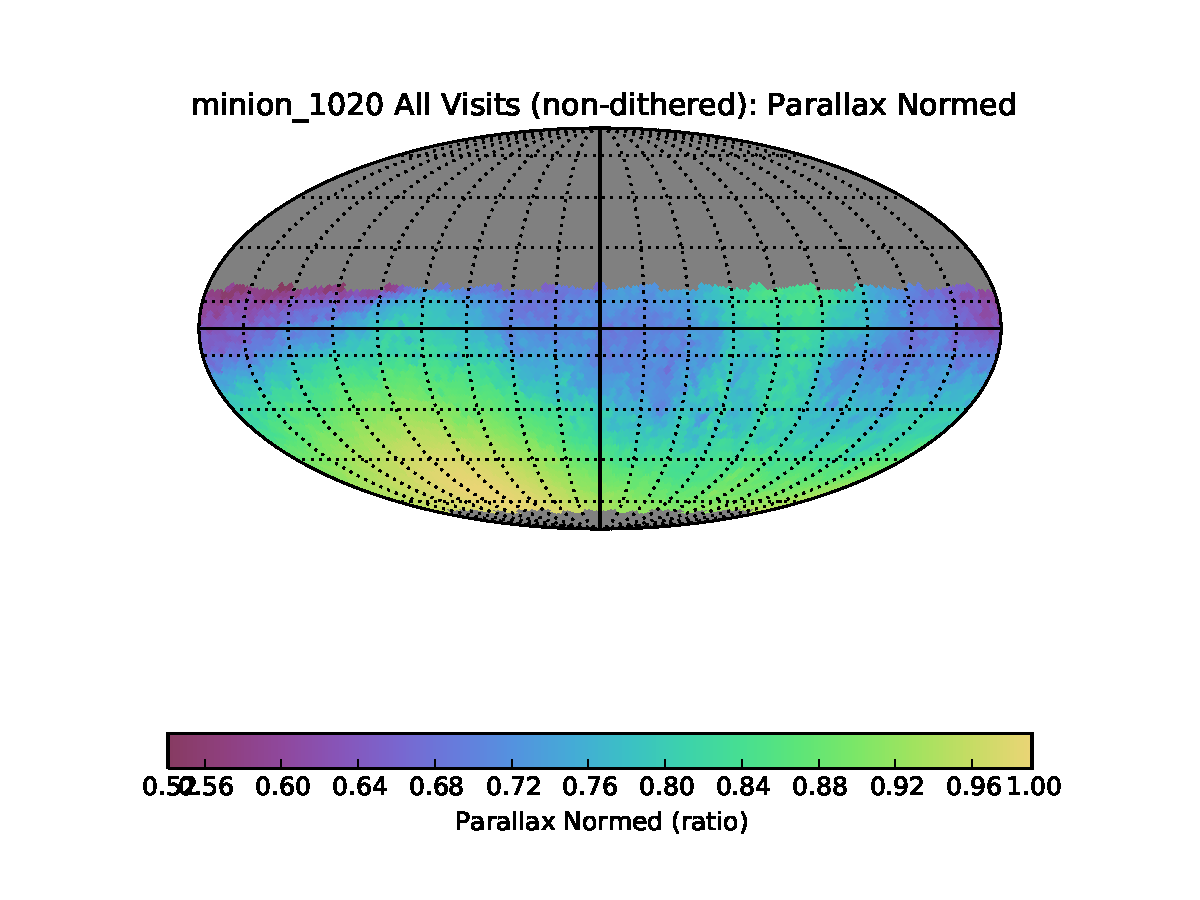
\includegraphics[angle=0,width=0.49\hsize:,clip]{figs/cadence/minion_1020_Parallax_Normed_All_Visits_non-dithered_HEAL_SkyMap.pdf}
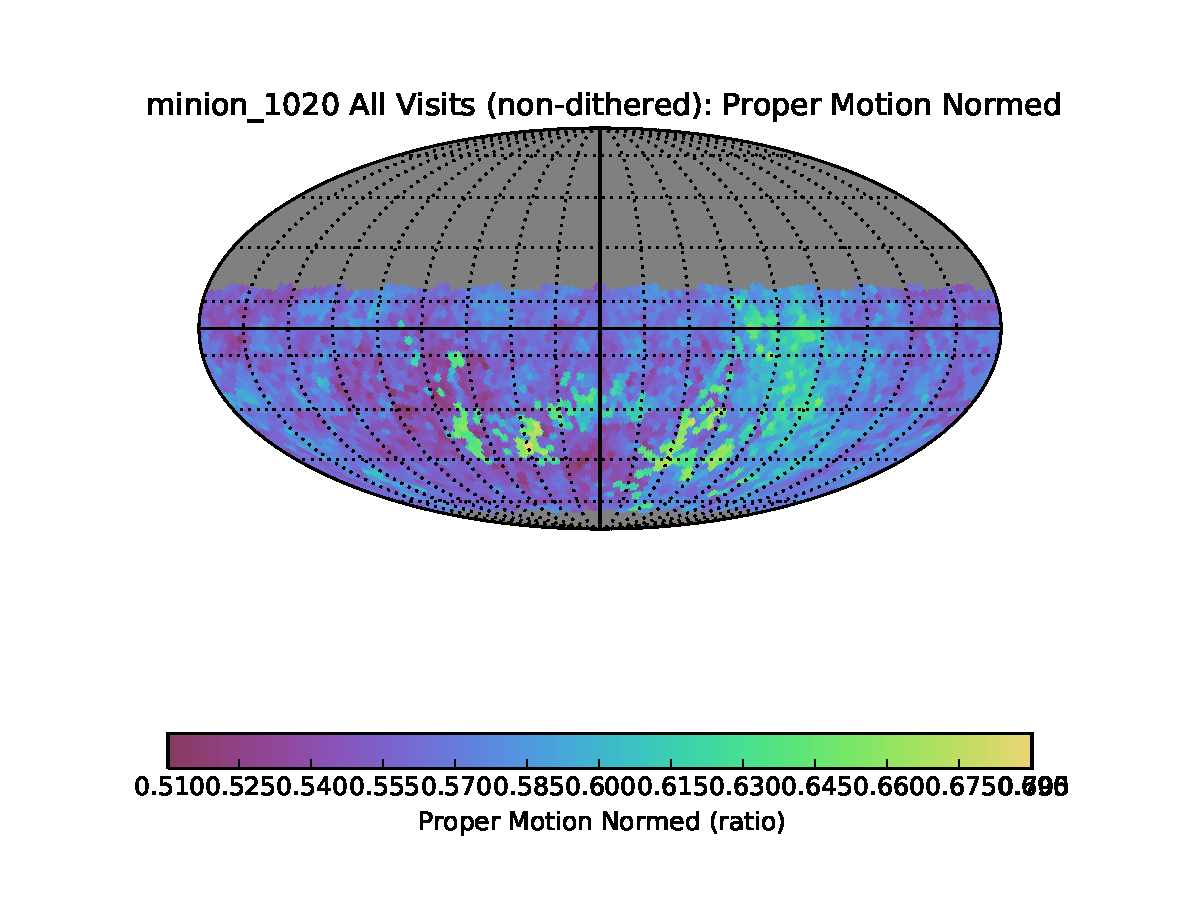
\includegraphics[angle=0,width=0.49\hsize:,clip]{figs/cadence/minion_1020_Proper_Motion_Normed_All_Visits_non-dithered_HEAL_SkyMap.pdf}
\vskip -0.2in
\caption{The trigonometric parallax errors (left) and proper motion errors (right)  for simulated cadence
minion\_1020 (``Pan-STARRS-like'' cadence), normalized by the values for idealized perfectly optimized
cadence, are shown in Aitoff projection of equatorial coordinates (compare to \autoref{fig:parapmenigma}).}
\label{fig:parapmenigma2}
\end{figure}
%%%%%%%%%%%%%%%%%%%%%%%%%%%%%%%%%

%%%%%%%%%%%%%%%%%%%%%%%%%%%%%%%%%
\begin{figure}[t!]
\vskip -0.03in
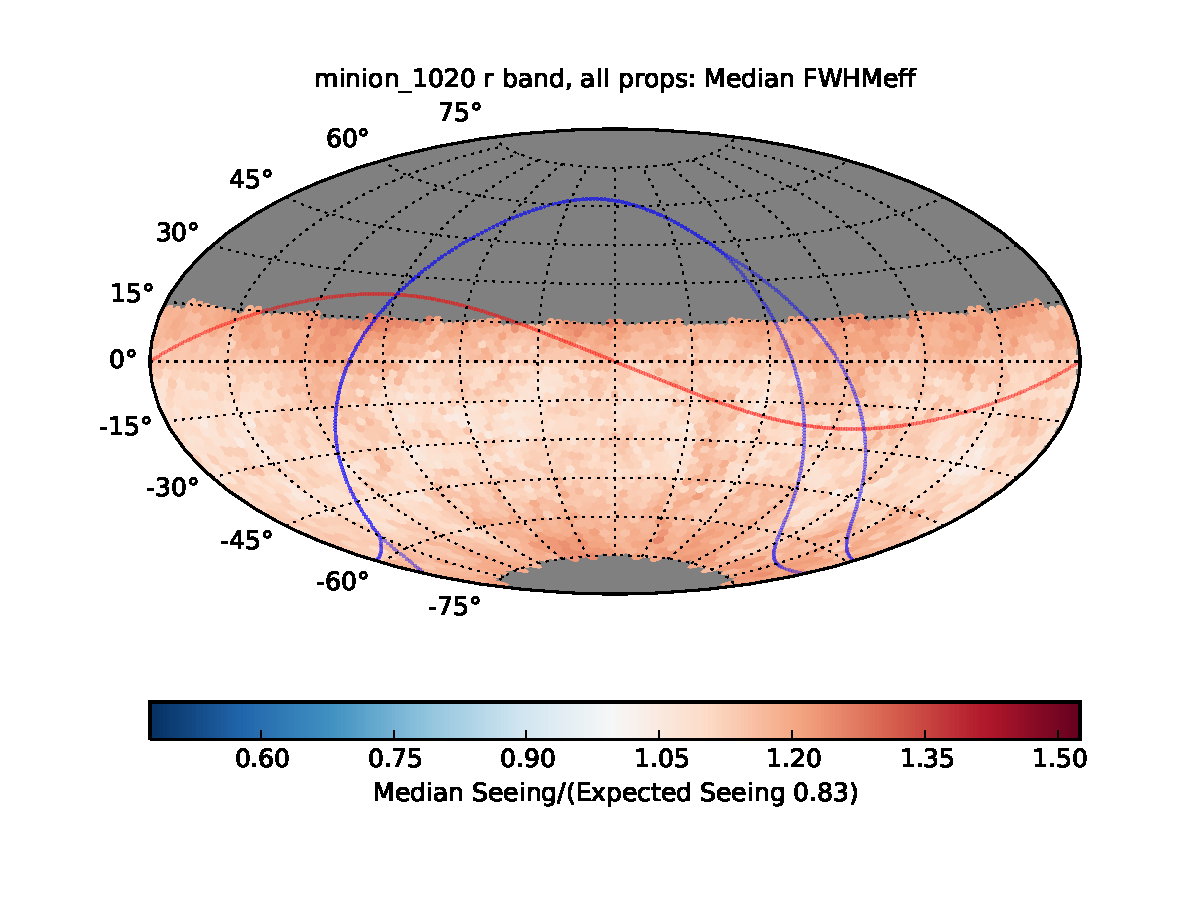
\includegraphics[angle=0,width=0.49\hsize:,clip]{figs/cadence/minion_1020_Median_FWHMeff_r_band_all_props_OPSI_SkyMap.pdf}
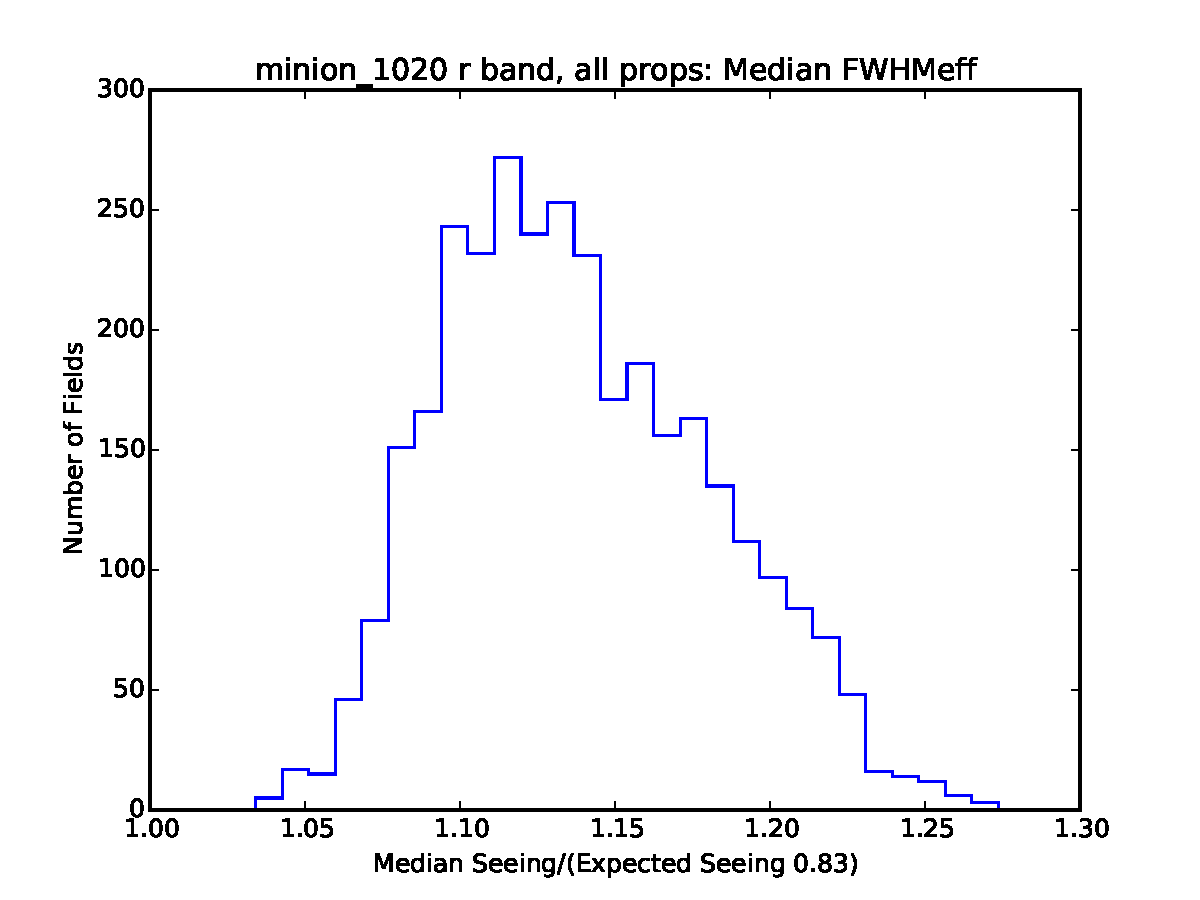
\includegraphics[angle=0,width=0.49\hsize:,clip]{figs/cadence/minion_1020_Median_FWHMeff_r_band_all_props_OPSI_Histogram.pdf}
\vskip -0.2in
\caption{The median seeing in $r$ filter, for simulated cadence minion\_1020 (``Pan-STARRS-like'' cadence),
normalized by expected value (0.83$^{\prime\prime}$). Note that fields with the most positive and most negative
declination have on average larger values. For comparison, the median normalized seeing for WFD fields
in Baseline Cadence is 1.08, with a negligible fraction of fields with values above 1.18.}
\label{fig:PS-seeing}
\end{figure}
%%%%%%%%%%%%%%%%%%%%%%%%%%%%%%%%%


% - - - - - - - - - - - - - - - - - - - - - - - - - - - - - - - - - -

%%%%%%%%%%%%%%%%%%%%%%%%%%%%%%%%%%%%%%%%%%%
\opsimdb[db:UConlyNoVisitPairs]{minion\_1013}{Only Universal Cadence, no visit pairs.}
%%%%%%%%%%%%%%%%%%%%%%%%%%%%%%%%%%%%%%%%%%%

{\bf Motivation and description:} The main goal of this simulation was
to assess the impact of the requirement for visit pairs on the survey
efficiency (Baseline Cadence requests two visits per night to the same
field, separated in time by about an hour, and driven by asteroid
orbit determination). It is plausible that the removal of this
requirement could result in a more efficient survey. In order to allow
as simple analysis as possible, only the Universal Cadence proposal is
requested. Hence, this simulation should be directly compared to
simulation \opsimdbref{db:opstwo}. \\

{\bf Expectations:} If the requirement for visit pairs decreases
surveying efficiency, then this simulation should deliver more than
2.45 million visits delivered by \opsimdbref{db:opstwo}. \\

{\bf Analysis Results:} This simulated cadence is named \opsimdbref{db:UConlyNoVisitPairs}. Compared
to \opsimdbref{db:opstwo}:
\begin{enumerate}
\item The total number of visits is 2.45 million, identical to \opsimdbref{db:opstwo}.
\item The median slew time, and the median coadded depth and seeing in the $r$ band
are essentially identical, too.
\item The median airmass in the $r$ band of 1.26 is a bit higher than 1.20 obtained
for \opsimdbref{db:opstwo}.
\item The median fraction of revisits faster than 30 minutes of 0.35 is smaller than 0.39
for \opsimdbref{db:opstwo}, and is consistent with the absence of pair contributions (that is,
such revisits are due to field edge overlaps, and unintentional revisits, in case of \opsimdbref{db:UConlyNoVisitPairs}).
\end{enumerate}

{\bf Conclusions:} The comparison of this simulation and
\opsimdbref{db:opstwo} shows that requiring pairs of visits (in a
given observing night) does not result in an appreciable loss of
surveying efficiency. Indeed, pairs of visits result in a better
short-timescale coverage that would enhance many types of time-domain
science (and, of course, it's crucial for asteroid science).


% - - - - - - - - - - - - - - - - - - - - - - - - - - - - - - - - - -

%%%%%%%%%%%%%%%%%%%%%%%%%%%%%%%%%%%%%%%%%%%
\opsimdb[db:NoVisitPairs]{kraken\_1043}{Baseline Cadence, but with no visit pairs.}
%%%%%%%%%%%%%%%%%%%%%%%%%%%%%%%%%%%%%%%%%%%

{\bf Motivation and description:} The main goal of this simulation was
to assess the impact of the requirement for visit pairs on the survey
efficiency. Instead of the idealized case above which compared only
the Universal Cadence proposal fields, in this more realistic case
{\it all proposals from Baseline Cadence are executed}. Hence, this
simulation should be compared to Baseline Cadence
(\opsimdbref{db:baseCadence}). \\

{\bf Expectations:} A slight, or no, increase in surveying efficiency
and thus the total number of visits is expected when compared to
Baseline Cadence. \\

{\bf Analysis Results:}  This simulated cadence is named
\opsimdbref{db:NoVisitPairs}. Compared to \opsimdbref{db:baseCadence},
\begin{enumerate}
\item The total number of visits is 2.53 million, or 2.4\% more than
in Baseline Cadence.
\item The mean slew time is 5.8 sec, or 16\% shorter than for Baseline
Cadence. This decrease in the mean slew time implies an efficiency
increase of 2.8\% and explains the actual 2.4\% improvement implied by
the total number of visits.  Note that this simulation has the
shortest mean slew time of all simulations investigated here (the
nominal shortest slew and settle time is about 4.5 sec).
\item The median airmass in the r band is slightly larger for this
simulation than for Baseline Cadence: 1.29 vs. 1.23.
\end{enumerate}


{\bf Conclusions:}
Unlike the comparison of \opsimdbref{db:UConlyNoVisitPairs} and
\opsimdbref{db:opstwo}, here the removal of visit pair requirement
results in a 16\% shorter mean slew time and consequently in 2.4\%
more visits.

% - - - - - - - - - - - - - - - - - - - - - - - - - - - - - - - - - -

%%%%%%%%%%%%%%%%%%%%%%%%%%%%%%%%%%%%%%%%%%%
\opsimdb[db:ShortExptime]{kraken\_1052}{Baseline Cadence, but with 33\% shorter exposure time.}
%%%%%%%%%%%%%%%%%%%%%%%%%%%%%%%%%%%%%%%%%%%

{\bf Motivation and description:} The optimal exposure time per visit
for the main survey, in the limit of a single value for all bands and
at all times, is in the range of about 20--60 seconds (see Section
2.2.2 in the LSST overview paper, arXiv:0805.2366, version 3.1). This
simulation investigates the effect of decreasing the exposure time per
visit to 20 seconds (from its nominal value of 30 seconds). The
shorter exposure time results in 0.22 mag shallower faint limit per
visit (the effect is larger in the $u$-band, see
\opsimdbref{db:DoubleUbandExptime}). \\

{\bf Expectations:} The total number of visits is expected to increase
by about 50\%, compared to \opsimdbref{db:baseCadence}, to 3.70 million,
for the same survey efficiency. However, the shorter exposure time
will have a significant impact on the survey efficiency: assuming a
slew time of 7 sec, the efficiency drops from 73\% to 65\% (comparing
30/(30+4+7) vs. 20/(20+4+7)). Therefore, the expected increase in the
number of visits is about 32\% and the expected number of visits is
3.2 million.  \\

{\bf Analysis Results:}  This simulated cadence is named
\opsimdbref{db:ShortExptime}. Compared to Baseline Cadence:
\begin{enumerate}
\item The total number of visits is 3.29 million, representing an
increase of 33\% that is very close to the expected value of 32\%.
\item The median number of visits per night is 1091, or about 34\%
more than for Baseline Cadence. The total open shutter time is 11\%
smaller for this simulation, and easily understood as due to expected
11\% decrease due to smaller surveying efficiency (the mean slew time
is practically the same as in Baseline Cadence, 6.8 sec vs. 6.9 sec).
\item The main survey (WFD, 18,000 sq. deg.) fields received 32\% more
visits than in Baseline Cadence. The increase in the minimum number of
visits over that area is 7\% (from 898 to 961). In addition, another
1,000 sq. deg. (6\% of the nominal WFD) area has more than 961 visits.
\item Most other performance parameters are essentially unchanged: the
fraction of visits spent on the main survey (84\% vs. 85\%), the
median seeing in the r band (0.78 arcsec vs. 0.77 arcsec), and the
median airmass (1.24 vs. 1.23).
\end{enumerate}

{\bf Conclusions:}
The comparison of \opsimdbref{db:ShortExptime} and
\opsimdbref{db:baseCadence} simulations demonstrates that the effect of
shorter exposures can be easily understood using simple efficiency
estimates. With the visit exposure time is decreased from 30 sec to 20
sec, the surveying efficiency and the total open shutter time drops by
$\sim$10\%, while the number of (shorter exposure time) visits (for
all proposals) increases by 33\%.



% - - - - - - - - - - - - - - - - - - - - - - - - - - - - - - - - - -

%%%%%%%%%%%%%%%%%%%%%%%%%%%%%%%%%%%%%%%%%%%
\opsimdb[db:LongExptime]{kraken\_1053}{Baseline Cadence, but 100\% longer exposure time.}
%%%%%%%%%%%%%%%%%%%%%%%%%%%%%%%%%%%%%%%%%%%

{\bf Motivation and description:} This simulation investigates the
effect of increasing the exposure time per visit to 60 seconds (from
its nominal value of 30 seconds). The longer exposure time results in
0.38 mag deeper faint limit per visit (the effect is larger in the
$u$-band, see \opsimdbref{db:DoubleUbandExptime}). \\

{\bf Expectations:} The total number of visits is expected to decrease by about
a factor of 2 in case of no significant impact on the survey efficiency.
However, the longer exposure time improves efficiency by a factor of
$2\times(34+7)/(64+7)-1=15\%$, and thus the expected total number of visits is
$0.5\times1.15 = 58\%$ of the number of visits in Baseline Cadence (assuming
the same mean slew time of 7 seconds).

{\bf Analysis Results:} This simulated cadence is named \opsimdbref{db:LongExptime}.
Compared to Baseline Cadence:
\begin{enumerate}
\item The total number of visits is 1.42 million or 58\% of the visits
obtained with Baseline Cadence, and the total open-shutter time is
15\% higher than for Baseline Cadence. Both results are in good
agreement with above expectations.
\item The median number of visits per night is 472, or 58\% of the
value obtained with Baseline Cadence. The mean slew time is 0.1 sec
longer than that obtained with Baseline Cadence.
\item This simulation has significantly different time allocation per
proposal, compared to Baseline Cadence: 69\% spent on the Universal
proposal (vs. 85\%) and 18\%  spent on the North Ecliptic proposal
(vs. 6\%)  (with smaller and less important differences for other
proposals). Because of these differences, {\it the results of this
test may not be very robust.}
\end{enumerate}

{\bf Conclusions:}
Simple estimates of the total number of visits and the improvement in
efficiency are in good agreement with delivered values. Of course, the
increased efficiency comes at the cost of fewer visits, which is
disadvantageous for time-domain science.

{\bf Note to OpSim team: this simulation should be repeated} with the
requested number of visits per field set to 60\% of the values used
for Baseline Cadence for {\bf all} proposals. For example, instead of
(75, 105, 240, 240, 210, 210) for Universal-18-0824B proposal, (45,
63, 144, 144, 126, 126) should be used.  This way the additional
observing time due to improved surveying efficiency will be allocated
to all proposals, including Universal Cadence. {\it This simulation
will be repeated with the same North Ecliptic Spur proposal as used
for \opsimdbref{db:baseCadence}, and with the modified requested number of
visits.}


% - - - - - - - - - - - - - - - - - - - - - - - - - - - - - - - - - -

%%%%%%%%%%%%%%%%%%%%%%%%%%%%%%%%%%%%%%%%%%%
\opsimdb[db:DoubleUbandExptime]{kraken\_1045}{Baseline Cadence, but with doubled $u$-band exposure time.}
%%%%%%%%%%%%%%%%%%%%%%%%%%%%%%%%%%%%%%%%%%%

{\bf Motivation and description:} The read-out noise in the u band is
not negligible compared to the background noise as in other bands, due
to darker u band sky. The current best estimates for survey
performance (see Table 2 in the LSST overview paper, arXiv:0805.2366,
version 3.1) indicate that the {\it coadded} depth in the $u$ band
could be improved by 0.24 mag by increasing the exposure time per
visit from 30 seconds to 60 seconds\footnote{In the background-limited
case, a factor of two increase of the exposure time results in 0.38
mag deeper data. Since in the u band the read-out noise is not
negligible compared to the background noise, the total noise increases
by less than a factor of $\sqrt{2}$ and there is an extra depth
improvement of 0.24 mag (see eq.~7 and Table 2 the overview paper).
Conversely, when exposure time is shorter than 30 seconds, there is an
extra penalty of 0.16 mag, in addition to a loss of depth of 0.22 mag
due to shorter exposure time in the limit of negligible read-out
noise.} (assuming the same total exposure time, which implies a
decrease in the number of visits by a factor of two). To keep the
total exposure time in the $u$ band unchanged, the requested number of
visits in this simulation is decreased by a factor of 2 relative to
Baseline Cadence specification. \\

{\bf Expectations:} The total exposure time in the u band should
remain unchanged. The single visits depth should be 0.38 mag deeper
due to twice as long exposure time (the gain of 0.24 mag related to
read-out noise effects is not yet implemented in the \OpSim code so MAF
outputs may be a bit confusing). \\

{\bf Analysis Results:} This simulated cadence is named \opsimdbref{db:DoubleUbandExptime}.  Compared
to Baseline Cadence (\opsimdbref{db:baseCadence}):
\begin{enumerate}
\item The total number of visits is 2.21 million or 89.5\% of the
Baseline Cadence values. The fraction of time allocated to the main
survey is 77\% vs. 85\% for Baseline Cadence, and for the NE spur
proposal 14\% vs. 6\%. Given that the NE spur proposal was different
than for \opsimdbref{db:baseCadence}, this simulation needs to be rerun.
\end{enumerate}

{\bf Conclusions:} The u band exposure time can be increased from 30
seconds to 60 seconds without a significant impact on the survey
efficiency. This change would result in a gain of about 0.2 mag in the
coadded depth. However, the number of visits in the u band would be
decreased by about a factor of two, with a negative impact on
time-domain science.  {\it This simulation will be repeated with the
same North Ecliptic Spur proposal as used for \opsimdbref{db:baseCadence}
to make conclusions more robust and precise.}

% - - - - - - - - - - - - - - - - - - - - - - - - - - - - - - - - - -

%%%%%%%%%%%%%%%%%%%%%%%%%%%%%%%%%%%%%%%%%%%
\opsimdb[db:DoubleUbandExptimewithNESpur]{kraken\_1059}{Baseline Cadence, but with doubled $u$-band exp.\ time and Baseline NE Spur.}
%%%%%%%%%%%%%%%%%%%%%%%%%%%%%%%%%%%%%%%%%%%

{\bf Motivation and description:} This simulation is similar to
\opsimdbref{db:DoubleUbandExptime}, which increased the exposure time
per visit in the $u$-band from 30 seconds to 60 seconds, with the
requested number of visits decreased by a factor of 2. This change
resulted in a gain of about 0.24 mag in the coadded depth. Since the
number of $u$ band visits in \opsimdbref{db:DoubleUbandExptime} was
decreased by about a factor of two, with a negative impact on
time-domain science, this simulation does not change the nominal
requested number of visits per field. Hence, the coadded depth in the
u band in this simulation would be improved by about 0.6 mag. \\

{\bf Expectations:}  Given that about 5\% of all visits are allocated
to the $u$ band, the total number of visits may decrease by up to
about 5\%, resulting in about 0.03 mag shallower data in bands other
than u band. \\

{\bf Analysis Results:}  This simulated cadence is named
\opsimdbref{db:DoubleUbandExptimewithNESpur}.  Compared to Baseline
Cadence (\opsimdbref{db:baseCadence}):
\begin{enumerate}
\item The total number of visits is 2.36 million or 95.5\% of the
Baseline Cadence values. The fraction of time allocated to the main
survey is 78\% vs. 85\% for Baseline Cadence, and for the NE spur
proposal 13\% vs. 6\%. Given that the NE spur proposal was different
than for \opsimdbref{db:baseCadence}, this simulation needs to be rerun.
\end{enumerate}


{\bf Conclusions:} When the $u$ band exposure time is increased from
30 seconds to 60 seconds, and the number of visits is kept unchanged,
the single-visit and coadded depths would be improved by 0.6 mag. This
improvement would come at  the expense of about 6\% fewer visits in
other bands (with about 0.03 mag shallower coadded depths).

% - - - - - - - - - - - - - - - - - - - - - - - - - - - - - - - - - -

%%%%%%%%%%%%%%%%%%%%%%%%%%%%%%%%%%%%%%%%%%%
\opsimdb[db:UConlyRelaxedAirmass]{minion\_1022}{Only Universal Cadence, with relaxed airmass limit.}

%%%%%%%%%%%%%%%%%%%%%%%%%%%%%%%%%%%%%%%%%%%

{\bf Motivation and description:}  What is the effect of changing the
airmass limit from 1.5 to 2.0?  To avoid complicated analysis, use
only Universal Cadence proposal and thus compare to
\opsimdbref{db:opstwo}.


{\bf Analysis Results:}  This simulated cadence is named
\opsimdbref{db:UConlyRelaxedAirmass}.  Compared to
\opsimdbref{db:opstwo}, it collected 98.0\% visits. This fraction is
identical to the loss of efficiency due to slightly longer mean slew
time: 8.1 sec vs. 7.2 sec. In addition,
\opsimdbref{db:UConlyRelaxedAirmass} has much worse airmass
distributions than \opsimdbref{db:opstwo},  extending to the allowed
maximum of 2.0. For example, the median for the r band and WFD fields
is 1.33, compared to 1.20 for \opsimdbref{db:opstwo}.

{\bf Conclusions:} This simulation confirms that it's a bad idea to
relax airmass limit: as a result, the airmass distribution always
widens. In addition, relaxed airmass limit tends to result in a longer
mean slew time.  For a given proposal, the airmass limit has to be as
tight as possible, while still allowing observations of all requested
fields.


% - - - - - - - - - - - - - - - - - - - - - - - - - - - - - - - - - -

%%%%%%%%%%%%%%%%%%%%%%%%%%%%%%%%%%%%%%%%%%%%%%%
\opsimdb[db:UConlyStringentAirmass]{minion\_1017}{Only Universal Cadence, with stringent airmass limit.}
%%%%%%%%%%%%%%%%%%%%%%%%%%%%%%%%%%%%%%%%%%%%%%%

{\bf Motivation and description:} What is the effect of changing the
airmass limit from 1.5 to 1.3? To avoid complicated analysis, we use
only the Universal Cadence proposal and thus compare to
\opsimdbref{db:opstwo}.

 {\bf Analysis Results:}  This simulated cadence is named
 \opsimdbref{db:UConlyStringentAirmass}. Compared to
 \opsimdbref{db:opstwo}, it collected essentially the same number of
 visits. The mean slew time is also essentially unchanged (7.4 sec vs.
 7.2 sec). The airmass distributions is improved compared to
 \opsimdbref{db:opstwo}. For example, the median for the r band and
 WFD fields is 1.14, compared to 1.20 for \opsimdbref{db:opstwo}.  The
 limiting coadded depth in u and g bands is about 0.1 mag deeper than
 for Baseline Cadence.

{\bf Conclusions:}  It is possible to achieve the same surveying
efficiency with much more stringent airmass limit than 1.5, which was
used in most simulations to date.  {\it Given this encouraging
behavior, an analogous experiment should be executed for Baseline
Cadence (i.e.\ a simulation like \opsimdbref{db:baseCadence}, with airmass
limit for the main survey set to 1.3) -- after the ``Western bias'' is
fixed'.}

\navigationbar

% --------------------------------------------------------------------

\section{Analysis of NEO/PHA completeness}
\def\secname{cadexp:NEOs}\label{sec:\secname}

% \noindent{\it Analysis of NEO/PHA completeness:   ops2\_1094, enigma\_1258, enigma\_1259}

Continuing our analysis of some alternatives to the Baseline Cadence,
we now investigate a suite of observing strategies for their
suitability in supporting Near-Earth Object (NEO) science. As in the
previous section, these \OpSim databases are all available for further
testing with science-based MAF metrics.

The U.S. Congress has given a mandate to NASA to implement a
Near-Earth Object (NEO) Survey program to detect, track, catalog,
and characterize the physical characteristics of near-Earth objects
equal to or greater than 140 meters in diameter\footnote{See
\url{http://www.gpo.gov/fdsys/pkg/PLAW-109publ155/pdf/PLAW-109publ155.pdf}}.
The goal is to achieve a completeness of 90\%. In recent practice,
adopted here, the completeness is evaluated for a subset of NEOs
called Potentially Hazardous Asteroids\footnote{Potentially Hazardous
Asteroids (PHAs) are defined as asteroids with a minimum orbit
intersection distance (MOID) of 0.05 AU or less.}  (PHA), with
H$\le$22, where H is the absolute magnitude\footnote{Absolute
magnitude is the magnitude that an asteroid would have at a distance
of 1 AU from the Sun and from the Earth, viewed at zero phase angle.
This is an impossible configuration, of course, but the definition is
motivated by desire to separate asteroid physical characteristics from
the observing configuration.} in the Johnson's V band. While LSST is
very competitive in this context, it will also enable analysis of many
other Solar System populations (e.g.\ main-belt asteroids, comets,
trans-Neptunian objects). Nevertheless, we focus our analysis here on
NEOs/PHAs completeness.


{\bf Motivation and description:}\\
The baseline cadence implements observing strategy with two visits to
a field obtained per night, separated in time by a fraction of an
hour. Motivation for a simulation that does require pairs of visits is
to gauge its impact on the survey efficiency and other performance
parameters. Motivation for simulations with more than two visits to a
given field per night is to investigate the feasibility of a more
robust approach to linking individual detections into a plausible
object track. Although detailed simulations of the performance of
image differencing software and orbital determination software
indicate that two visits per night are likely to be sufficient,
quantitative analysis of other strategies is clearly within the
purview of the cadence optimization program.  Five simulations are
analyzed in this section:


% - - - - - - - - - - - - - - - - - - - - - - - - - - - - - - - - - -

%%%%%%%%%%%%%%%%%%%%%%%%%%%%%%%%%%%%%%%%%%%
\opsimdb[db:NEOsNoVisitPairs]{kraken\_1043}{NEO test: no request for pairs of visits.}
%%%%%%%%%%%%%%%%%%%%%%%%%%%%%%%%%%%%%%%%%%%

% - - - - - - - - - - - - - - - - - - - - - - - - - - - - - - - - - -

%%%%%%%%%%%%%%%%%%%%%%%%%%%%%%%%%%%%%%%%%%%
\opsimdb[db:NEOswithVisitPairs]{enigma\_1016}{NEO test: pairs of visits
  (i.e.\ the Baseline Cadence).}.
%%%%%%%%%%%%%%%%%%%%%%%%%%%%%%%%%%%%%%%%%%%

% - - - - - - - - - - - - - - - - - - - - - - - - - - - - - - - - - -

%%%%%%%%%%%%%%%%%%%%%%%%%%%%%%%%%%%%%%%%%%%
\opsimdb[db:NEOswithVisitTriplets]{enigma\_1281}{NEO test: triplets of visits.}

%%%%%%%%%%%%%%%%%%%%%%%%%%%%%%%%%%%%%%%%%%%

% - - - - - - - - - - - - - - - - - - - - - - - - - - - - - - - - - -

%%%%%%%%%%%%%%%%%%%%%%%%%%%%%%%%%%%%%%%%%%%
\opsimdb[db:NEOwithVisitQuads]{enigma\_1282}{NEO test: quads of visits.}

%%%%%%%%%%%%%%%%%%%%%%%%%%%%%%%%%%%%%%%%%%%

% - - - - - - - - - - - - - - - - - - - - - - - - - - - - - - - - - -

{\bf Expectations:}  Analysis of all simulations is repeated three
times, with different conditions for what constitutes an object's
``discovery'':  two, three or four detections per night are required,
together with at least three such sequences in a 15-day window.  When
only two detections per night are required, a modest decrease in PHA
completeness is expected for simulations that request more than two
visits per night because some visits ``don't live up to their full
potential''. On the other hand, when more than two detections per
night are required, a naive expectation is that PHA completeness for
runs with fewer requested visits will drop significantly. \\

%%%%%%%%%%%%%%%%%%%%%%%%%%%
\begin{figure}[t!]
\vskip -2.5in
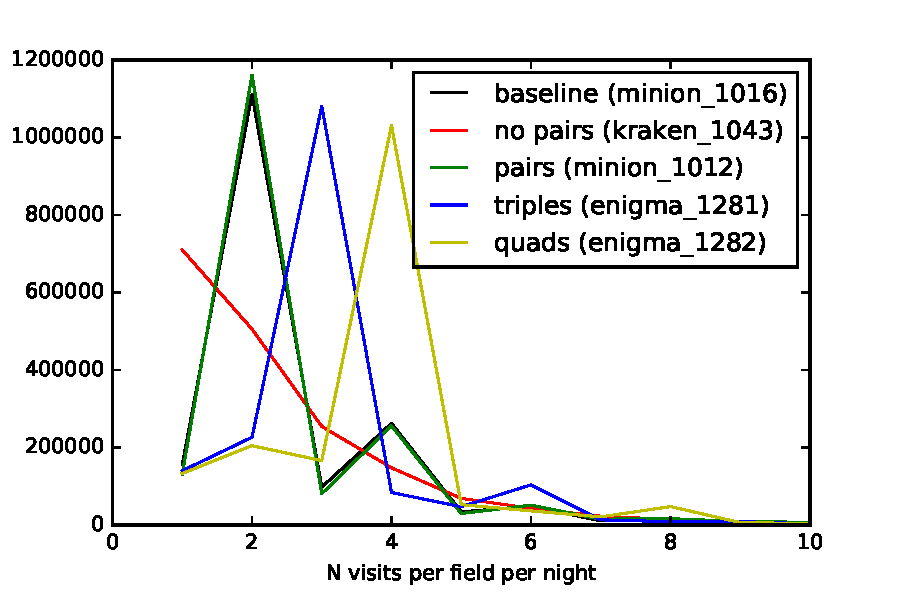
\includegraphics[angle=0,width=0.99\hsize:,clip]{figs/NvisitStats.pdf}
\vskip -2.7in
\caption{The distribution of the number of visits used for nightly sequences of
length given on the horizontal axis. Only $griz$ bands are used. Note that even
``no pairs'' simulation (\opsimdbref{db:NEOsNoVisitPairs})
includes multiple visits. The highest peak is at the
requested number of visits in a sequence.}
\label{fig:NvisitStats}
\end{figure}
%%%%%%%%%%%%%%%%%%%%%%%%%%%

%%%%%%%%%%%%%%%%%%%%%%%%%%%
\begin{figure}[t!]
\vskip -1.2in
\includegraphics[angle=0,width=0.49\hsize:,clip]{figs/medinternight1.pdf}
\includegraphics[angle=0,width=0.49\hsize:,clip]{figs/medinternight2.pdf}
\vskip -1.3in
\caption{%
The comparison of the median intra-night gap distributions for Baseline Cadence (left)
and simulation \opsimdbref{db:NEOsNoVisitPairs}, which did not request pairs of visits per night.
Despite no need for pairs, simulation \opsimdbref{db:NEOsNoVisitPairs} produced them ``spontaneously'',
as well as longer sequences (see \autoref{fig:NvisitStats}). The mean field revisit
time is much shorter (about 6 minutes, see the right panel) than for Baseline Cadence
(22 minutes).}
\label{fig:intranightgapCompare}
\end{figure}
%%%%%%%%%%%%%%%%%%%%%%%%%%%

%%%%%%%%%%%%%%%%%%%%%%%%%%%
\begin{figure}[t!]
\vskip -1.1in
\includegraphics[angle=0,width=0.56\hsize:,clip]{figs/enigma1189_diffNEOcompleteness.pdf}
\hskip -0.5in
\includegraphics[angle=0,width=0.56\hsize:,clip]{figs/enigma1189_cumNEOcompleteness.pdf}
\vskip -1.2in
\caption{The PHA completeness for \opsimdbref{db:baseCadence}, as a function of the object's absolute
visual magnitude H on the horizontal axes (left: differential completeness at a given H;
right: cumulative completeness for all objects brighter than a given H).
The completeness for H$\le$22 NEOs (those with diameters larger than 140m)  for this
simulation is 73\% (blue line in the right panel). The panels also show the effects of ignoring
chip gaps (a 2\% effect for cumulative H$\le$22 completeness) and of decreasing the
field-of-view size to a half (i.e.\ to 4.8 sq.\ deg; a 10\% effect).}
\label{fig:enigmaNEO}
\end{figure}
%%%%%%%%%%%%%%%%%%%%%%%%%%%

%%%%%%%%%%%%%%%%%%%%%%%%%%%
\begin{figure}[th!]
\vskip -1.2in
\includegraphics[angle=0,width=0.49\hsize:,clip]{figs/diffNEOpairs.pdf}
\includegraphics[angle=0,width=0.49\hsize:,clip]{figs/diffNEOquads.pdf}
\vskip -1.3in
\caption{%
The comparison of differential PHA completeness for the five analyzed simulations
when requiring two detections per night (left) and four detections per night (right).
With two detections per night, all simulations perform similarly but when four
detections per night are required, the simulation that has the largest number
of such sequences (see \autoref{fig:NvisitStats}), performs the best although at an
inferior level compared to the left panel (see also \autoref{fig:enigmaNEO}).}
\label{fig:NEOquads}
\end{figure}
%%%%%%%%%%%%%%%%%%%%%%%%%%%


{\bf Analysis Results:}
First, we emphasize that ``requested'' is not the same as
``delivered'': even the ``no pairs''
simulation \opsimdbref{db:NEOsNoVisitPairs} ends
up having multiple visits in a given night to the same fields, and
when multiple visits per night are requested, not all fields get to
have completed sequences. The statistics of how many fields are
combined into sequences of a given number of visits is shown in
\autoref{fig:NvisitStats}.  As evident, the highest peak is at the
requested number of visits in a sequence, but not all visits are
incorporated into requested sequences: some are in both shorter and
longer sequences. In particular, even ``no pairs'' simulation includes
multiple visits to some fields, essentially because the current
version of the algorithm is not told not to do so. As illustrated in
\autoref{fig:intranightgapCompare}, such revisits typically happen
within 10 minutes from the first visit. This (unintended) behavior
implies that the naive expectation above is probably incorrect, as we
discuss in more detail below.


For baseline reference, the PHA completeness for
\opsimdbref{db:baseCadence} is shown in \autoref{fig:enigmaNEO}. The
baseline cadence achieves a cumulative completeness of 73\% for
H$\le$22 PHAs. This cumulative completeness for H$\le$22 is 17\%
higher than differential completeness at H=22 of 56\% due to
increasing completeness towards smaller H (larger objects). Both
differential and cumulative completeness are relevant metrics: the
former provides more insight in the behavior of a particular
simulation, while the latter is a metric given to NASA by the U.S.
Congress. Analysis of results illustrated in \autoref{fig:NEOquads}
can be summarized as follows:
\begin{itemize}
\item When NEO discovery algorithm requires pairs of visits, all runs
have very similar PHA completeness, with quads run only about 2\%
lower than the baseline (a differential completeness of 56\% at H=22
for \opsimdbref{db:baseCadence})
\item When NEO discovery algorithm requires 4 detections per night,
the simulation with quads achieves a differential completeness of
about 27\% at H=22, or  about 30\% lower completeness than Baseline
Cadence.
\item When NEO discovery algorithm requires 4 detections per night,
Baseline Cadence reaches a differential completeness of about 15\% at
H=22 (some quads are unintentionally produced by chance, see
\autoref{fig:NvisitStats}).
\item When NEO discovery algorithm requires 3 detections per night,
runs which requested triples and quads achieve a differential
completeness of about 40\% at H=22 (corresponding to a cumulative
completeness of about 57\% for H$\le$22).
\end{itemize}

Therefore, going from pairs of visits to triples (both for cadence and
NEO detection) reduces completeness (both differential and cumulative)
for PHAs with H$\le$22 by about 15-20\% (and by about 30\% for quads).


\subsubsection{Impact on other science programs}

The impact of requesting sequences with 3 or 4 visits to the same
field on other science programs is not yet analyzed in detail.  The
impact on static science should be minimal, except perhaps for a bit
worse behavior of various systematic errors (because fewer nights,
with their observing conditions, are sampled).

For time-domain science, the mean revisit time will increase by about
50\% if we go from pairs to triples, and by about a factor of two for
quads. This change will have a negative impact on time-domain science
programs based on SNe, variable stars, and transient objects, which
remains to be quantified.

\navigationbar

% --------------------------------------------------------------------



% ====================================================================
% commands for stand-alone printing
%\documentclass[11pt,headsepline,cleardoubleempty,twoside,openright]{scrbook}
%\usepackage{SciBook}
%\begin{document}
% ====================================================================

% ====================================================================
%+
% NAME:
%    rollingcadence.tex
%
% ELEVATOR PITCH:
%    TODO: Explain in a few sentences what the relevant discovery or
%    measurement is going to be discussed, and what will be important
%    about it. This is for the browsing reader to get a quick feel
%    for what this section is about.
%
% COMMENTS:
%
%
% BUGS:
%
%
% AUTHORS:
%    Steve Ridgway (@StephenRidgway)
%-
% ====================================================================

\section{ Rolling Cadence }
\def\secname{rolling}\label{sec:\secname}

\noindent{\it Stephen Ridgway, \ldots} % (Writing team)

% This individual section will need to describe the particular
% discoveries and measurements that are being targeted in this section's
% science case. It will be helpful to think of a ``science case" as a
% ``science project" that the authors {\it actually plan to do}. Then,
% the sections can follow the tried and tested format of an observing
% proposal: a brief description of the investigation, with references,
% followed by a technical feasibility piece. This latter part will need
% to be quantified using the MAF framework, via a set of metrics that
% need to be computed for any given observing strategy to quantify its
% impact on the described science case. Ideally, these metrics would be
% combined in a well-motivated figure of merit. The section can conclude
% with a discussion of any risks that have been identified, and how
% these could be mitigated.

With a total of ~800 visits spaced approximately uniformly over 10 years, and distributed among 6 filters,
it is not clear that LSST can offer the sufficiently dense sampling in time for study of transients with typical durations less than or $\simeq 1$week.
This is particularly a concern for key science requiring well-sampled SNIa light curves.  Rolling cadences stand out as a
general solution that can potentially enhance sampling rates by 2$\times$ or more, on some of the sky all of the time and all of the sky some of the time, while maintaining a sufficient uniformity for survey objectives that require it.

\subsection{The Uniform Cadence}

Current schedule simulations allocate visits as pairs separated by 30-60 minutes, for the purposes of identifying asteroids.  For most science purposes, the 30-60 minute spacing is too small to reveal temporal information, and a pair will constitute effectively a single epoch of measurement.  If the expected 824 (design value) LSST visits are realized as 412 pairs, and distributed uniformly over 10 observing seasons of 6 months each, the typical separation between epochs will be 4 days.   The most numerous visits will be in the {\it r} and {\it i} filters, and the repeat visit rate in either of these will be $\simeq$ 20 days.

The possibility is still open that, for asteroid identification, visits might be required as triples or quadrupoles, in which case the universal temporal sampling will be further slowed by 1.5 or 2$\times$.

Under a strict universal cadence it is not possible to satisfy a need for more frequent sample epochs.  This leads the simulations group to investigate the options opened up by reinterpreting the concept of a universal cadence.  Instead of aiming for a strategy which attempts to observe all fields ``equally'' all the time, it would allow significant deviations from equal coverage during the survey, returning to balance at the end of the survey.

Stronger divergence from a universal cadence, allowing significant inhomogeneities to remain at the end of the survey, is of course possible, but is not under investigation or discussed here.

There is currently considerable interest in the community in strategies that provide enhanced sampling over a selected area of the sky, and rotating the selected area in order to exercise enhanced sampling over all of the survey area part of the time.  The class of cadences that provides such intervals of enhanced visits, with the focus region shifting from time to time, is termed here a rolling cadence.  As a point of terminology, observing a single sky area with enhanced cadence for a period of time will be described as a ``roll''.

\subsection{Rolling Cadence Basics}

Assume a fixed number of observing epochs for each point on the sky, nominally distributed uniformly over the survey duration.  A subset of these can be reallocated to provide improved sampling of a sky region.  This will have the inevitable effects of: (1) reducing the number of epochs available for that sky region during the rest of the survey, and (2) displace observations of other sky regions during the time of the improved temporal sampling.  In short, the cadence outside the enhanced interval will be degraded.

The essential parameters of rolling cadence are: (1) the number of samples taken from the uniform cadence, and (2) the enhancement factor for the observing rate.  The LSST document 16370, ``A Rolling Cadence Strategy for the Operations Simulator'', by K. Cook and S. Ridgway,  contains more detailed discussion and analysis.

\begin{figure}
  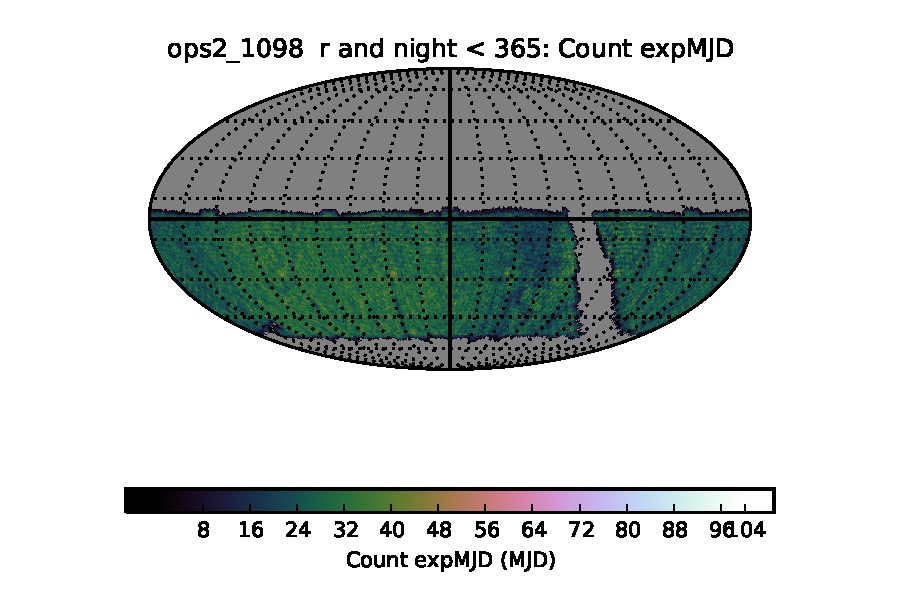
\includegraphics[width=2.3in]{figs/ops2_1098_Count_expMJD_r_and_night_lt_365_HEAL_SkyMap.pdf}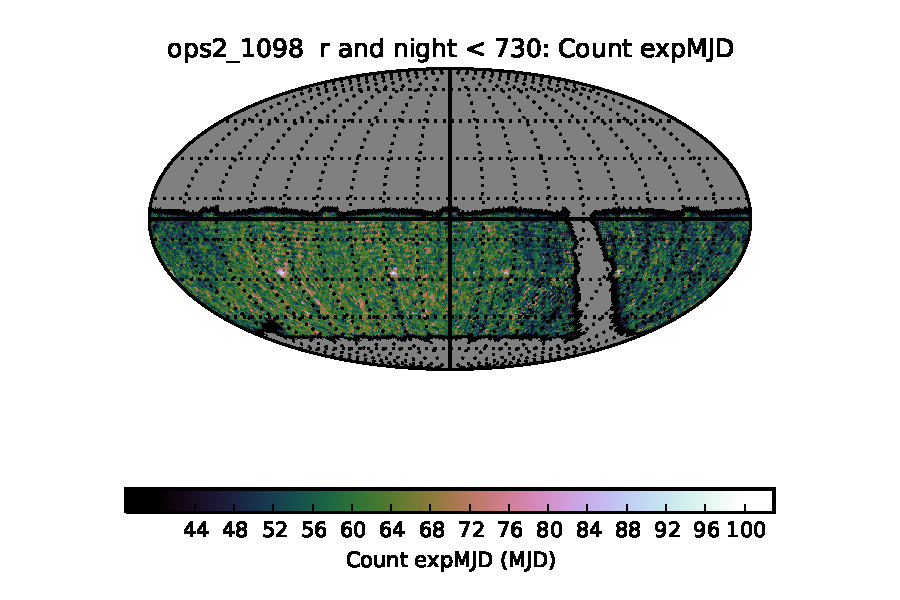
\includegraphics[width=2.3in]{figs/ops2_1098_Count_expMJD_r_and_night_lt_730_HEAL_SkyMap.pdf}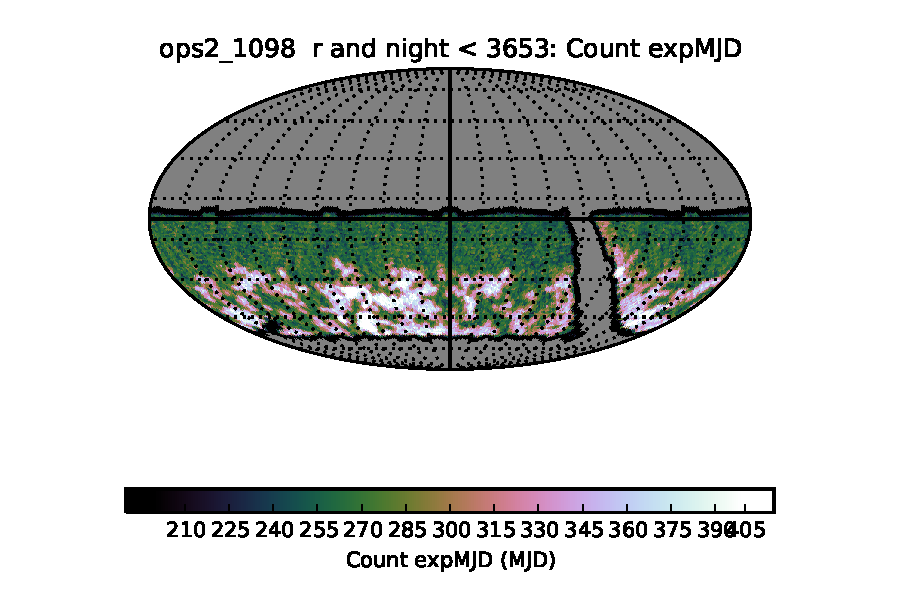
\includegraphics[width=2.3in]{figs/ops2_1098_Count_expMJD_r_and_night_lt_3653_HEAL_SkyMap.pdf} \\
  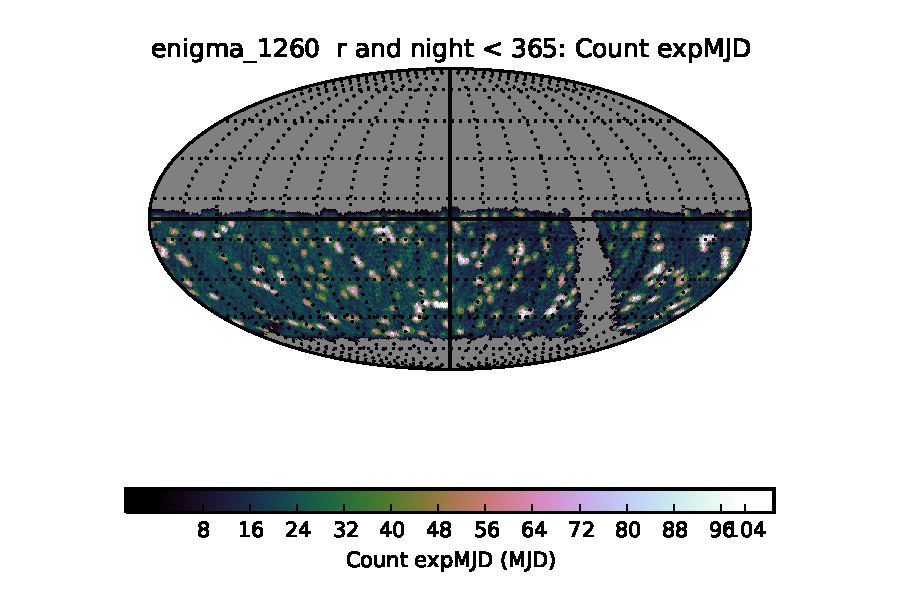
\includegraphics[width=2.3in]{figs/enigma_1260_Count_expMJD_r_and_night_lt_365_HEAL_SkyMap.pdf}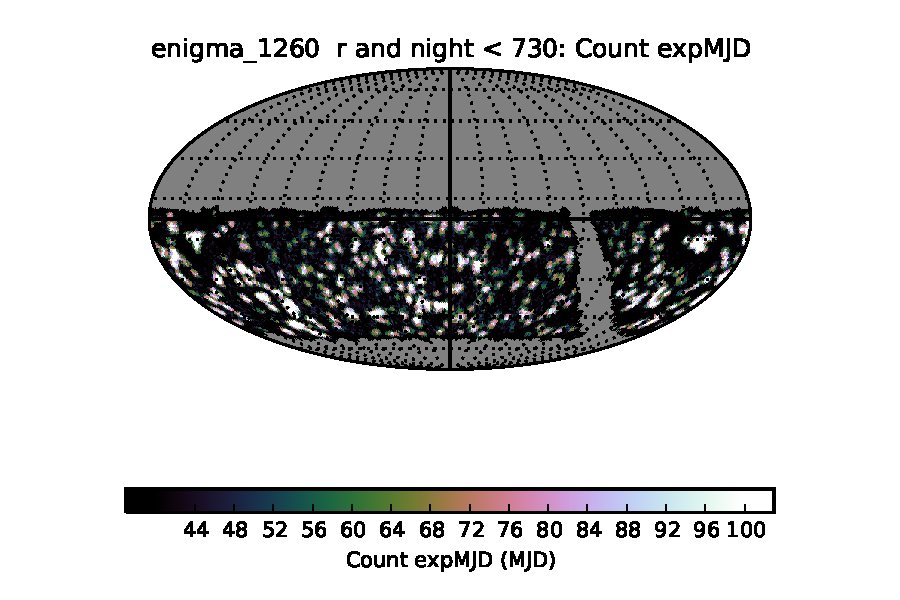
\includegraphics[width=2.3in]{figs/enigma_1260_Count_expMJD_r_and_night_lt_730_HEAL_SkyMap.pdf}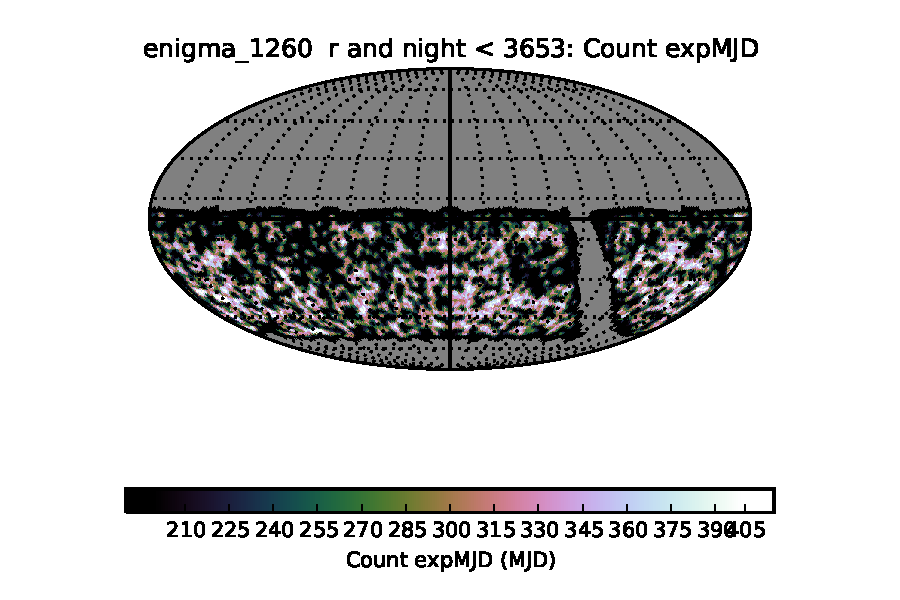
\includegraphics[width=2.3in]{figs/enigma_1260_Count_expMJD_r_and_night_lt_3653_HEAL_SkyMap.pdf}
  \caption{Example of a regular uniform survey (top) and a rolling cadence survey (bottom) after 1, 2, and 10 years in the $r$ filter.  For the regular survey, the number of visits for any part of the sky is relatively constant throughout the survey.  For the rolling cadence simulation, there are regions with many more exposures in year one which then fade in year two as other parts of the sky are emphasized.\label{fig:rollingcadence}}
\end{figure}

% --------------------------------------------------------------------
% --------------------------------------------------------------------
\subsection{ Supernovae and Rolling Cadence}
\label{sec:rolling:supernovae}

\noindent{\it Author Name(s)} % (Writing team)

Supernovae as a science topic are addressed elsewhere.
In this section, the demands of SN are used to directly constrain or
orient the rolling cadence development.

Pending more quantitative guidance, the SN objective for rolling cadence is to obtain multicolor time series significantly longer than the typical SN duration, with a cadence significantly faster than uniform.  As an example we discuss the option of a rolling cadence with the regular distribution of filters.

As a simple example, consider improving the cadence by a factor of 2 or 3.  Is we accept that some regions of the sky will be enhanced every year, and that uniform sky coverage will only arrive at the end of 10 years, then we could use, e.g., 10\% of the total epochs in a single roll.  If the enhancement is 2$\times$, each roll would last for $\simeq$ 6 months, with high efficiency for capture of complete SN events.  If the enhancement is 4$\times$, each roll would last for 2 months, with lower efficiency.

If it is important to achieve survey uniformity after 3 years, the available visits for each roll would be reduced also.  With a 2$\times$ enhancement of epoch frequency, a roll would last 2 months.

Some leverage would be gained by using more than 10\% of the available visits for a single roll.  However, this begins to impact the sampling of slow variables reduce schedule flexibility and robustness, and should be approached with caution.

From these examples, it appears that a 2$\times$ enhancement with uniformity closure after 10 years is relatively feasible and promising.  Much higher gains, or more rapid closure, require additional compromises.

% --------------------------------------------------------------------

\subsection{ Fast Transients and Rolling Cadence}
\label{sec:rolling:transients}

\noindent{\it Author Name(s)} % (Writing team)

Fast transients as a science topic are addressed elsewhere. In this section, the demands of fast transients are used to directly constrain or
orient the rolling cadence development.

By ``fast transients'', we are referring to events that are sufficiently fast that they are not addressed by the rolling cadence designed for SN observations, and slow enough that they are not covered in ``deep drilling'' type mini-surveys.  For higher tempo rolls, it is quite difficult to obtain full color data, because of the constraints on filter selection.  For this example, we will examine a rolling cadence utilizing only the {\it r} and {\it i} filters, as they are used for most visits. They are close in wavelength, and we assume that sufficient color information will be obtained by the ``background'' uniform survey that continues during a roll.

Again using 10\% of the available visits from the full 10 year survey for a single roll, we find that there would be enough epochs for each roll to acquire 1 visit per day for 21 consecutive days, giving an enhancement of 10$\times$.

Alternatively, the same epochs could be used to observe a target every 20 minutes for 12 hours during a single night (here it is assumed that visit pairs are not required, doubling the available epochs) for an enhancement of 300$\times$.

Several different possible redeployments of portions of a uniform survey have been described, each using 10\% of available time.  Of course it is possible in principal to implement multiple options, sequentially or maybe in parallel in some cases. This may pose considerable challenges to the scheduling strategy design by introducing incompatible boundary conditions.

While rolling cadences are powerful, they have limitations.  For example, sampling events that last longer than $\simeq$1 day and less than $\simeq$ 1 week have the obvious problem of diurnal availability.  In this example, intermediate cadences could be implemented in the circumpolar region, where diurnal access is much extended.  This is an example of a case in which a mini-survey of a limited number of regions could be considered as an alternative to a rolling cadence applied to the entire main survey.

% --------------------------------------------------------------------

\subsection{ Constraints, Trades and Compromises for Rolling Cadences}
\label{sec:rolling:trades}

While rolling cadences offer some attractive benefits, it is important to realize that rolling cadences are very highly constrained, and that they do bring disadvantages and compromises.

There are strong arguments against beginning a rolling cadence in the first, or even the second year of the survey.  Early in the survey, it is important to obtain for each field/filter combination, an adequate number of good quality photometric images, and at least one image in excellent seeing, to support closure of photometry reductions and to support generation of template images.

Since major science goals require a significant degree of survey homogeneity, it may be advisable to implement a strategy that brings the survey to nominal uniform depth at several times, e.g. after 3 or 5 years.  This would strongly constrain rolling cadences.

Some science objectives favor certain distributions of visits.  For astrometry, visits early and late in the survey and at large parallax factors, are beneficial.  Slow variables may benefit from uniform spacing.  Rolling cadences might impact these constraints either favorably or unfavorably.

Many objectives are served by randomization of observing conditions for each field.  Some rolling cadences could tend to reduce this randomization, for example by acquiring a large number of observations during a meteorologically favorable or unfavorable season, or during a period of instrument performance variance.

Dithering does not work gracefully with a rolling cadence, reducing temporal coverage at the boundaries of the selected sky region.  This is negligible for small dithers, but important for large dithers, which are under consideration.

These cautions illustrate that evaluation of rolling cadences must be based on the full range of schedule performance metrics, and not just those targeted by rolling cadence development.

% ====================================================================

\navigationbar

% ====================================================================
% commands for stand-alone printing
% \bibliographystyle{apj}
% \bibliography{references}
% \end{document}
% ====================================================================


% --------------------------------------------------------------------

\section{Ongoing and Future Work}
\def\secname{cadexp:ongoing}\label{sec:\secname}


\subsection{Ongoing: Extended time-domain metrics}

A number of very sophisticated time-domain metrics have been
implemented in recent MAF development cycle (and some were contributed
by the community) but they have not been systematically run yet on all
available simulations. Time-domain metrics, together with metrics for
analyzing special programs (e.g. deep drilling programs), will be
further expanded in the next development cycle.


\subsection{Ongoing: Rolling Cadence experiments}

Analysis of a few prototype runs (\texttt{ops2\_1102},
\texttt{enigma\_1260}, \texttt{enigma\_1261}), which implemented the
so-called ``swiss cheese rolling cadence'' is in progress.


\subsection{Future work}

Based on analysis presented here, several recommendations
for further cadence exploration, can be made.

\begin{enumerate}

\item Further optimization of the main survey (e.g., exposure time in
general, and u band exposure time in particular; fixing western bias;
optimizing airmass limit and sky coverage; investigations of variable,
perhaps SNR-driven, exposure time).

\item Exploration and optimization of temporal sampling function in
general, and of Rolling Cadence in particular.

\item NEO completeness studies: what would it take for LSST to reach
90\% completeness for 140m and larger NEOs?  Based on previous
analysis, directions to explore are deeper visits along the Ecliptic
and longer survey duration (about 12 years).

\item Exploration of extending the main survey to the Galactic plane
(per A. Gould's proposal, arXiv:1304.3455) and further optimization of
Galactic plane and Bulge science programs.

\item Optimization of LMC/SMC coverage (and somewhat less importantly,
the South Celestial Pole coverage).

\item Deep drilling optimization (detailed analysis of existing
proposals; investigation of gains from going to a larger observing
time allocation, e.g. 20\%).

\item Twilight short-exposure time observing (per internal Stubbs proposal).

\item Planning commissioning observations (e.g. the tension between
going wide to enable self-calibration and dense temporal sampling to
obtain various light curve templates and fine tune image differencing
and multi-epoch data processing and data analysis software tools).

\item Dynamic cadence explorations (the main goal at this time is to
answer: are our tools good enough to act and react swiftly and
robustly in operations?).

\end{enumerate}

\navigationbar

% --------------------------------------------------------------------

\section{Summary}
\def\secname{cadexp:summary}\label{sec:\secname}

The most important conclusion of this study is that the upper limit on
possible scheduling efficiency improvements for Baseline Cadence is
close to 6\%. This conclusion is by and large based on the fact that
the mean slew time for (candidate) Baseline Cadence is 6.9 sec, and
thus only slightly larger than the design specifications for the
system slew and settle time of 4.5 sec.  Nevertheless, there are a
number of features to understand, and some to fix, and there is
substantial optimization potential in temporal sampling functions and
further optimization of the sky area and observing strategy details,
that can result in enhanced science even with the same integrated
open-shutter time (e.g. by obtaining deeper data through an improved
sampling of observing conditions).

\vskip 0.2in
The main other questions addressed here are:

\begin{enumerate}

\item {\it By what factor could we exceed the SRD design specification
for the number of visits if only Universal Cadence proposal was
implemented?}

A simulation that only implemented Universal Cadence proposal exceeded
the design specification for the number of visits by about 40\% (over
the design specification for the sky area of 18,000 sq.deg.)

\item {\it By what factor could we exceed the SRD design specification
for the sky coverage if only Universal Cadence proposal was
implemented with the design specification for the number of visits?}

This Pan-STARRS-like strategy results in about 40\% larger sky
coverage (about 25,000 sq.deg.), with the mean number of visits at
92\% of the design specification. The total number of visits is the
same as for Baseline Cadence, implying similar surveying efficiency.

Therefore, the available ``margin'' relative to the SRD design specifications
for the main survey is equivalent to about 30-40\% larger sky coverage, or
about 30-40\% more visits per field. The SRD assumes that 10\% margin
will be available for other programs. The implied ``survey reserve'',
relative to the Universal Cadence design specifications from the SRD, can
be used to:
  \begin{enumerate}
  \item increase the number of visits per field over the WFD area,  or
  \item increase the surveyed area while keeping the number of visits
  per field statistically unchanged, or
  \item increase both area and the number of visits, and/or
  \item execute additional programs (the current baseline).
  \end{enumerate}

\item {\it What is the effect of auxiliary proposals on surveying
efficiency?}

A comparison of simulations which only implemented Universal Cadence
proposal to those that included all other programs did not show a
significant change of efficiency (older simulations, not analyzed
here, showed increases in surveying efficiency of up to about 3\% due
to shorter slewing time).


\item {\it What is the effect of visit pairs on surveying efficiency? }

Relinquishing the visit pair requirement results in up to 2-3\%
improvement of the surveying efficiency. The impact on some
time-domain science would be positive, while for NEO and main-belt
asteroid science it would be strongly negative.


\item {\it Can the effects of variations of the visit exposure time on
surveying efficiency be predicted using simple efficiency estimates?}

Simple estimates based on comparing exposure (open shutter) and total
visit times are in good agreement with simulations. Decreasing the
visit exposure time to 20 seconds decreases the total open shutter
time by 10\%, and increasing it to 60 seconds increases the total open
shutter time by 16\%, relative to Baseline Cadence and standard
exposure time of 30 seconds. The number of visits changes by factors
of 1.35 and 0.58.


\item {\it What are the effects of doubling the exposure time only in
the $u$ band?}

The effect of doubling the exposure time only in the $u$ band, while
simultaneously halving the number of requested visits, has no
significant effect on the survey efficiency.

The effect of doubling the exposure time only in the $u$ band, with
the number of requested visits unchanged, is a decrease in the number
of visits in other bands by about 6\%.


\item {\it What is the impact of hard airmass limit, $X<1.5$, on the
surveying efficiency?}

It is a very bad idea to relax airmass limit! It is possible to
achieve the same surveying efficiency with much more stringent airmass
limit than 1.5, which was used in most simulations to date.

\end{enumerate}


\navigationbar

%%  LocalWords:  STARRS cadexp Bremerton MAF opsim baseCadence Aitoff
%%  LocalWords:  airmass coadded WFD Msec airmassenigma ugrizy ivezic
%%  LocalWords:  SRD coaddm urz ury parapmenigma OpSim pre HAenigma
%%  LocalWords:  AltAzenigma radians enigmaGapAll enigmaGapr SNe griz
%%  LocalWords:  enigmaMAXGapAll enigmaEarlySNe Intra opstwoPS opstwo
%%  LocalWords:  UConlyNoVisitPairs NoVisitPairs kraken ShortExptime
%%  LocalWords:  DoubleUbandExptime LongExptime UConlyRelaxedAirmass
%%  LocalWords:  DoubleUbandExptimewithNESpur UConlyStringentAirmass
%%  LocalWords:  NEO PHA NEOs PHAs MOID Neptunian detections intra eq
%%  LocalWords:  differencing NEOsNoVisitPairs NEOswithVisitPairs LMC
%%  LocalWords:  NEOswithVisitTriplets NEOwithVisitQuads NvisitStats
%%  LocalWords:  enigmaNEO intranightgapCompare NEOquads Gould's SMC
%%  LocalWords:  Stubbs multi yoachim rhiannonlynne quartiles swiss
%%  LocalWords:  strawman unrequested


% --------------------------------------------------------------------

\chapter[Solar System]{Discovering and Characterizing Small Bodies in
  the Solar System}
\def\chpname{solarsystem}\label{chp:\chpname}

Chapter editors:
\credit{rhiannonlynne},
\credit{davidtrilling}.

% ====================================================================

\section{Introduction}
\label{sec:\chpname:intro}

LSST has tremendous potential as a discovery and characterization tool
for small bodies in the Solar System. With LSST, we have the
opportunity to increase our sample sizes of Potentially Hazardous
Asteroids (PHAs), Near Earth Objects (NEOs), Main Belt Asteroids
(MBAs), Jupiter Trojans, Centaurs, TransNeptunian Objects (TNOs),
Scattered Disk Objects (SDOs), comets and other small body populations
such as Earth mini-moons, irregular satellites, and other planetary
Trojan populations, by at least an order of
magnitude, often two orders of magnitude or more. In addition to
hundreds of astrometric measurements for most objects, LSST will also
provide precisely calibrated multiband photometry. With this
information, we can also characterize these populations -- deriving
colors, light curves, rotation periods, spin states, and even shape
models where possible.

The motivation behind studying these small body populations is
fundamentally to understand planet formation and evolution. The
orbital parameters of these populations record traces of the orbital
evolution of the giant planets. The migration of Jupiter, Saturn and
Neptune in particular have left marks on the orbital distribution of
MBAs, Jupiter Trojans, TNOs and SDOs. Rapid migration of
Jupiter and Saturn may have emplaced a large number of planetesimals
in the Scattered Disk; later slow migration of Neptune will affect the
number of TNOs in resonance and the details of their orbital parameters
within the resonance. Adding color information provides further
insights; colors roughly track composition, indicating formation
location and temperature or space weathering history. For example, the color
gradient of main belt asteroids, combined with their orbital
distribution, suggests that perhaps Jupiter migrated inwards,
mixing planetesimals from the outer Solar System into the outer parts
of the main belt, before eventually migrating outwards. Studying the
size distribution of each of the small body populations themselves
provides more constraints on planetesimal formation; this is
complicated by the effects of dynamical stirring from the giant
planets, which can increase the rate of erosion vs. growth during
collisions, and by the existence of the remnants of collisions such as
collisional families in the main belt. The presence of binaries and range
of spin states and shapes provides further constraints on the history
of each population. The location
of the planets before migration, the amount of migration, and the size
distribution of the small bodies themselves (after detangling the
dynamical evolution) all tell a deeper story about how the planets in
the Solar System formed, and how our formation history fits into the
range of observed extrasolar planetary systems.

These Solar System populations are unique when compared to other
objects which will be investigated by LSST, due to the simple fact
that they move across the sky. Metrics to evaluate
LSST's performance for moving objects need to be based on `per object'
measurements, rather than at a series of points on the sky or per
field pointing. For all metrics discussed in this chapter, the orbit
of each object is integrated over the time of the simulated opsim
survey and the times when each object is visible are recorded; these
series of observations per object are then the basis for metric
evaluations.

% Introduce, with a very broad brush, this chapter's science projects,
% and why it makes sense for them to be considered together.

% ====================================================================

\section{Discovering and linking Solar System Objects}
\def\secname{\chpname:discovery}\label{sec:\secname}

Discovering, rather than simply detecting, small objects throughout
the Solar System requires unambiguously linking a series of detections
together into an orbit. The orbit provides the information necessary
to scientifically characterize the object itself and to understand the
population as a whole. Without orbits, the detections of Solar System
Objects (SSOs) by LSST will be of limited use; objects discovered with
other facilities could be followed up by LSST, but almost the entire
science benefit to planetary astronomy would be lost. Linking and
orbit determination for Solar System objects is similar to source
association for non-moving objects; it provides the means to identify
multiple detections as coming from a single object.

Therefore, the first concern regarding the Solar System is related
to the question ``Can we accurately link individual detections of moving objects into
orbits?''.  This requirement poses varying levels of difficulty as we
move from Near Earth Objects (NEOs) through the Main Belt Asteroids
(MBAs) and to TransNeptunian Objects (TNOs) and Scattered Disk Objects
(SDOs), as well as for comets and for other unusual but very
interesting populations such as Earth minimoons. Due to their small
heliocentric and geocentric distances, NEOs appear move with
relatively high velocities and are distributed over a large fraction
of the sky, far from the ecliptic plane. MBAs are densely distributed,
primarily within about 30 degrees of the ecliptic. TNOs and SDOs move
slowly, however short time intervals between repeat visits in each night may make these difficult
to link. Comets and Earth mini-moons may require more complicated
orbit fitting to allow for non-gravitational or geocentric
orbits. It also implies that we do not create false objects by
incorrectly linking detections and/or noise.

Much of the answer to this question comes down to the performance of
various pieces of LSST Data Management software. In particular,
important questions are the
rate of false positive detections resulting from difference imaging, the compute
limitations of the Moving Object Processing System (MOPS) to extend to high
apparent velocities, and the capability to unambiguously determine if
a linkage is `real' or not via orbit determination (done as part of
MOPS). Thus this question ranges beyond the limits of the OpSim simulated
surveys, but bears on the observing strategy requirements for
discovering Solar System Objects. An in-depth study of the performance
of difference imaging and MOPS is currently ongoing. However, we can
make a range of assumptions on how MOPS will perform and evaluate how
many and which objects can be linked under observational cadence, given those assumptions.


% --------------------------------------------------------------------

\subsection{Target measurements and discoveries}
\label{sec:\secname:targets}

The criteria for `discovery' with MOPS depends on the number
of observations of an object acquired per night, within some time
window (creating `tracklets'), repeated over a number of nights within window of some
days (creating `tracks'), linked into an orbit with a threshhold on
astrometric residuals. The current assumptions are that we can link
detections into orbits with 2 detections per night within 90 minutes,
repeated for 3 nights within 15 days. The additional assumptions are
that with these 6 observations, we will be able to create low-accuracy orbits that will suffice to link
additional observations obtained at later (or earlier, in the LSST
archive) times, and that that the orbit fitting will enable rejection
of mislinkages.

We can also set other requirements for discovery. Requiring 4
detections within 90 minutes is a fairly common discovery criteria for
NEO surveys, as it reduces the number of mislinked tracklets to almost
zero. We could also require 4 nights of pairs, in order to improve the
initial orbit fitting and mislinkage rejection.

With these discovery criteria, we can then evaluate the completeness
of an LSST simulated survey, for a given population. We can look at
this as a function of H magnitude and as a function of orbital
parameters.

For PHAs and NEOs there are special considerations in terms of
completion that arise from planetary defense concerns. For most other
populations, the general desire is simply to have a high level of
completeness, with no gaps in completeness that depend strongly on
orbital parameters. In particular, the desire is to be able to
calibrate any selection effects in discovery so that the survey completeness can
be used to debias the underlying population models.

Discovery opportunity, and thus the completeness of the underlying
population, is very sensitive to the time interval between
observations. For most solar system objects, with a 90 minute window
within a night, gathering two or more repeat observations within a night requires
that the field pointing is revisited two or more times. Gathering
observations over multiple nights for a wide variety of Solar System
objects (moving at a wide variety of apparent velocities) generally requires covering a large
neighboring area of sky; thus the internight revisit rate for large contiguous
blocks of sky is important. An optimal discovery strategy for moving
objects could be ensuring a minimum (default: two) number of revisits
within a night within a short time window (default: 90 minutes), and
covering large contiguous amounts of sky several (default: 3) times within a
longer time window (default: 15 days).

% --------------------------------------------------------------------

\subsection{Metrics}
\label{sec:\secname:metrics}

The {\tt Discovery Metric} can be used to identify sets of detections
of a particular object that meet the defined criteria for discovery: X
detections within TTI minutes in a night, Y nights within a W day
window; this describes the number of discovery opportunities for each object. The results from the Discovery Metric can be fed to the {\tt
  MO\_Completeness} summary metric, where if an object achieves a
user-defined requirement for the minimum number of discovery
opportunities (typically 1), then it is counted as `discovered'; then
the total number of objects discovered at each H magnitude is compared
to the total number of objects in the population at that H magnitude,
in order to evaluate `completeness' as a function of H. Discovery
opportunities can be evaluated as a function of orbital parameters, to
look for areas of orbital space that may be missed in a particular
survey strategy; completeness, since it marginalizes over the entire
population at a particular H value, loses this
capability. Completeness can be evaluated as a differential value
(completeness @ H=X) or integrated over the size distribution
(completeness @ H <= X).
 
A further simplification of the completeness can be achieved if the
completeness at a particular H magnitude is the desired value. For
example, completeness for PHAs at H=22 is an important summary value.

% --------------------------------------------------------------------

\subsection{OpSim Analysis}
\label{sec:\secname:analysis}

Put figures here ... 

OpSim analysis: how good would the default observing strategy be, at
the time of writing for this science project?


% --------------------------------------------------------------------

\subsection{Discussion}
\label{sec:\secname:discussion}

Discussion: what risks have been identified? What suggestions could be
made to improve this science project's figure of merit, and mitigate
the identified risks?



% ====================================================================

\section{Orbital Accuracy}
\def\secname{\chpname:orbits}\label{sec:\secname}


A short preamble goes here. What's the context for this science
project? Where does it fit in the big picture?

% --------------------------------------------------------------------

\subsection{Target measurements and discoveries}
\label{sec:\secname:targets}

Describe the discoveries and measurements you want to make.

Now, describe their response to the observing strategy. Qualitatively,
how will the science project be affected by the observing schedule and
conditions? In broad terms, how would we expect the observing strategy



% --------------------------------------------------------------------

\subsection{Metrics}
\label{sec:\secname:metrics}

Quantifying the response via MAF metrics: definition of the metrics,
and any derived overall figure of merit.


% --------------------------------------------------------------------

\subsection{OpSim Analysis}
\label{sec:\secname:analysis}

OpSim analysis: how good would the default observing strategy be, at
the time of writing for this science project?


% --------------------------------------------------------------------

\subsection{Discussion}
\label{sec:\secname:discussion}

Discussion: what risks have been identified? What suggestions could be
made to improve this science project's figure of merit, and mitigate
the identified risks?


% ====================================================================

\section{Detecting Activity}
\def\secname{\chpname:activity}\label{sec:\secname}


A short preamble goes here. What's the context for this science
project? Where does it fit in the big picture?

How secure is the orbit - is it going to hit us?
Libration amplitude distribution for TNOs?
Can we find it after X years for further study?
Can we identify the source region for NEOs within the main belt?

% --------------------------------------------------------------------

\subsection{Target measurements and discoveries}
\label{sec:\secname:targets}

Describe the discoveries and measurements you want to make.

Now, describe their response to the observing strategy. Qualitatively,
how will the science project be affected by the observing schedule and
conditions? In broad terms, how would we expect the observing strategy
to be optimized for this science?


% --------------------------------------------------------------------

\subsection{Metrics}
\label{sec:\secname:metrics}

Quantifying the response via MAF metrics: definition of the metrics,
and any derived overall figure of merit.


% --------------------------------------------------------------------

\subsection{OpSim Analysis}
\label{sec:\secname:analysis}

OpSim analysis: how good would the default observing strategy be, at
the time of writing for this science project?


% --------------------------------------------------------------------

\subsection{Discussion}
\label{sec:\secname:discussion}

Discussion: what risks have been identified? What suggestions could be
made to improve this science project's figure of merit, and mitigate
the identified risks?

Different discussion / risks for each science case within this general metric?

% ====================================================================

\section{Measuring colors}
\def\secname{\chpname:colors}\label{sec:\secname}


A short preamble goes here. What's the context for this science
project? Where does it fit in the big picture?

% --------------------------------------------------------------------

\subsection{Target measurements and discoveries}
\label{sec:\secname:targets}

Describe the discoveries and measurements you want to make.

Now, describe their response to the observing strategy. Qualitatively,
how will the science project be affected by the observing schedule and
conditions? In broad terms, how would we expect the observing strategy
to be optimized for this science?


% --------------------------------------------------------------------

\subsection{Metrics}
\label{sec:\secname:metrics}

Quantifying the response via MAF metrics: definition of the metrics,
and any derived overall figure of merit.


% --------------------------------------------------------------------

\subsection{OpSim Analysis}
\label{sec:\secname:analysis}

OpSim analysis: how good would the default observing strategy be, at
the time of writing for this science project?


% --------------------------------------------------------------------

\subsection{Discussion}
\label{sec:\secname:discussion}

Discussion: what risks have been identified? What suggestions could be
made to improve this science project's figure of merit, and mitigate
the identified risks?


% ====================================================================

\section{Measuring lightcurves/rotation periods}
\def\secname{\chpname:lightcurves}\label{sec:\secname}


A short preamble goes here. What's the context for this science
project? Where does it fit in the big picture?

% --------------------------------------------------------------------

\subsection{Target measurements and discoveries}
\label{sec:\secname:targets}

Describe the discoveries and measurements you want to make.

Now, describe their response to the observing strategy. Qualitatively,
how will the science project be affected by the observing schedule and
conditions? In broad terms, how would we expect the observing strategy
to be optimized for this science?


% --------------------------------------------------------------------

\subsection{Metrics}
\label{sec:\secname:metrics}

Quantifying the response via MAF metrics: definition of the metrics,
and any derived overall figure of merit.


% --------------------------------------------------------------------

\subsection{OpSim Analysis}
\label{sec:\secname:analysis}

OpSim analysis: how good would the default observing strategy be, at
the time of writing for this science project?


% --------------------------------------------------------------------

\subsection{Discussion}
\label{sec:\secname:discussion}

Discussion: what risks have been identified? What suggestions could be
made to improve this science project's figure of merit, and mitigate
the identified risks?


% ====================================================================


\navigationbar

% ====================================================================


% --------------------------------------------------------------------

% --------------------------------------------------------------------

\chapter{The Galaxy}
\def\chpname{galaxy}\label{chp:\chpname}

Chapter editors:
\credit{willclarkson},
\credit{akvivas}.

Contributing authors:
\credit{bethwillman},
\credit{dnidever},
\credit{ivezic},
\credit{ctslater},
\credit{pmmcgehee},
\credit{cbritt4},
\credit{dgmonet},
\credit{caprastro},
{\it Dana Casetti, John Gizis, Michael Liu and others to follow}


% --------------------------------------------------------------------

\section{Introduction}
\def\secname{MW_Intro}\label{sec:\secname}

LSST's large survey grasp will yield significant contributions to
essentially all areas of Galactic astronomy. Science cases for Milky
Way astronomy with LSST cover lengthscales from a few pc (such as
sensitive surveys of low-mass objects in the Solar Neighborhood), up
to many tens of kpc (such as sensitive surveys for low-mass satellite
galaxies of the Milky Way and their post-disruption remnant streams,
and beyond this, investigations of resolved stellar populations in the
Local Volume). 

Because the diversity of science cases in the Milky Way is so vast, we
make no attempt to be comprehensive. Much more detail about most of
the LSST science cases, and specific science questions to be answered,
can be found in the LSST Science Book (particularly chapters 6 and 7)
and Ivezic et al. (2008 arXiv 0805.2366, in particular Sections 2.1.4
and 4.4 of that document).\footnote{\new{Since several of the science cases for populations in the Galactic Disk do not appear to have been developed elsewhere, however, Section \ref{sec:MW_Disk} does present motivating details for those science cases.}} In this chapter we present a few
representative science cases that illustrate trade-offs between
observing strategies, for programs at low galactic latitudes as well
as away from the disk, and for programs requiring sufficient cadence
for variability as well as deep integrated imaging. 

As with the rest of this whitepaper, our intention is to provoke the
astronomical community to contribute to the optimization of LSST's
observing strategy. Readers who find that an important area of Milky
Way astronomy is under-served by the treatment here, are welcome to
contact the editors to get involved and contribute improvements. For
example, while inclusion of the inner Galactic plane in the
Wide-Fast-Deep survey would allow characterization of important
populations through variability (as will be shown quantitatively in
Section 4.3), such a dataset would also be of immense value in
disentangling and measuring structural parameters of major galactic
components (for example the tilt angle of the disk and the effects of
radial migration within it). We welcome further development of
quantitative figures of merit by which the appropriateness of LSST's observing
strategies can be assessed in terms of the science of interest to the
reader.

\subsection{Chapter terminology and structure}

In what follows, ``Metrics'' refer to diagnostic metrics of LSST's
technical performance, and are generally rather low-level (for
example, the formal proper motion precision, mapped with location
across the sky). Then, a ``figure of merit'' is a higher-level
quantity that illustrates LSST's utility for the science case of
interest (for example, the uncertainty and/or bias on an astrophysical
parameter of interest, such as the mass function of a certain stellar
population near the Sun).

To try to tame the diversity of science cases, we have picked
representative cases and grouped them within broad scientific areas,
devoting one Section of this chapter to each grouping of cases. Our
intention at this date is to provide a summary Table at the end of
each Section that will present the figure of merit for each science
case within that section (as columns) for each tested observing
strategy (as rows).

At present, science cases are grouped in the following way:
Section~\ref{sec:MW_Halo} assesses the degree to which structures in the Milky
Way's halo can be discriminated and mapped, using tracer populations
distinguished by variability and derived stellar parameters.
Section~\ref{sec:MW_Disk} assesses the impact of observing strategy on LSST's
ability to map some representative astrophysically important
populations that are found mostly or exclusively in the Plane
(including Dust in the ISM). Several observational challenges for LSST
find their sharpest expression in Milky Way science, including (but
not limited to) measurements of stellar parallax, absolute astrometry,
and proper motions (including the tie-in to the reference frame which
will be provided by the \textit{Gaia} mission). For this reason, specific
issues relating to precision astrometry are developed in
Section~\ref{sec:MW_Astrometry}.

%\new{(If there is time before posting:)} 
Section~\ref{sec:MW_Bulge} will describe two example uses of LSST to
set constraints on Galactic components (the structure of the Bulge,
and constraints on radial migration in the mid-plane), while
Section~\ref{sec:MW_LocalVolume} explores the use of LSST to probe the Local
Volume.

\subsection{Summary tables for Figures of Merit}

\new{At-a-glance tables comparing Figures of Merit for the various science
cases, will be found in the appropriate summary tables:}
\begin{itemize}
  \item Mapping the Milky Way Halo: Table \ref{tab_SummaryMWHalo}
    \item Mapping the Milky Way Disk: Table \ref{tab_SummaryMWDisk}
      \item Astrometry with LSST: Table \ref{tab_SummaryMWAstrometry}
        \item The Milky Way Bulge: content needed
          \item Mapping the Local Volume with Resolved Stars: content needed.   
\end{itemize}

\subsection{Needed input}

Many of the diagnostic Metrics are (as of February 2016) relatively
well-developed. What is needed at this stage is the implementation of
the figures of merit that depend on these Metrics. In some Sections we
have sketched out such figures of merit, in others the development of
a useful (and practical) figure of merit is still a topic of active
development. 

We welcome assistance from the reader in the development of the
figures of merit for all sections. 

% ====================================================================
%+
% SECTION:
%    section-name.tex  % eg lenstimedelays.tex
%
% CHAPTER:
%    chapter.tex  % eg cosmology.tex
%
% ELEVATOR PITCH:
%    Explain in a few sentences what the relevant discovery or
%    measurement is going to be discussed, and what will be important
%    about it. This is for the browsing reader to get a quick feel
%    for what this section is about.
%
% COMMENTS:
%
%
% BUGS:
%
%
% AUTHORS:
%    Phil Marshall (@drphilmarshall)  - put your name and GitHub username here!
%-
% ====================================================================

\section{Mapping the Milky Way Halo}
\def\secname{MW_Halo}\label{sec:\secname} % For example, replace "keyword" with "lenstimedelays"

\noindent{\it Kathy Vivas, Colin Slater, David Nidever, Beth Willman}  % (Writing team)

The study of the Halo of the Milky Way is of the most importance not only to understand
the formation and early evolution of our own galaxy, but also to test 
test current models of hierarchical galaxy formation. 
LSST will provide an unprecedented combination of
area, depth, multi-band, multi-epoch information for pursuing detail studies
of the structure of this old Galactic component. We focus here in three
specific projects that can be pursued with LSST. We suggest metrics and figure of merits that can
be calculated in order to quantify the feasibility of the projects under different
observational strategies. We expect more projects will join later.

RR Lyrae stars have been known for several decades as excellent tracers
of the halo population. They are not only old stars ($>10$ Gyrs) but they are
also excellent standard candles that allow to build 3-dimensional maps. 
The halo of the Milky Way has been now surveyed in a very large extension up to 
$\sim 60-80$ kpc from the Galactic center \citep[][among others]{drake13a,drake13b,zinn14,torrealba15}. 
Beyond that, the halo is
mostly uncharted territory.
From these RR Lyrae surveys, we have learned that the halo is filled with substructures
which are usually interpreted as debris from destroyed satellite galaxies. The smooth 
component of the RR Lyrae distribution is well described
with a power-law of the mean number density of RR Lyrae stars as a function of
galactocentric distance, which gets steeper after $\sim 30$ kpc \citep{zinn14}. 
Thus, beyond $\sim 60$ kpc, few field RR Lyrae stars are expected. However, we presume that 
any RR Lyrae star beyond this distance may be part of either debris material or distant
satellite galaxies of low luminosity that have been escaped detection until now \citep{sesar14,baker15}. 
LCDM models predict debris as far as $0.5$~Mpc from the galactic center
This is the territory that will be explored by LSST.

Similarly, red giant stars can be used to trace the structure of the halo up to large
distances. They have the advantage 
of being bright and numerous stars.

Fainter than these two tracers, main sequence stars stand up as a tool for studying
the Halo. They are the most numerous type of stars available and statistical studies 
are possible. Using the technique of photometric metallicities \citep{ivezic08}, 
SDSS provided unprecedented maps of the metallicity distribution up to  $\sim 10$ 
kpc from the Galactic center, unveiling not only the mean metallicity distribution 
of the halo but also, sub-structures within the halo. This kind of works will be extended
to the outermost parts of the Galaxy with LSST data.


% --------------------------------------------------------------------

\subsection{Target measurements and discoveries}
\label{sec:\secname:MW_Halo_targets}

The three projects just described require the discovery and/or measurement of the following 
type of objects:

\begin{itemize}

\item RR Lyrae stars: These are bright horizontal-branch variable stars with
periods between 0.2 to 1.0 days and large amplitudes, particularly in the bluer 
bandpasses (g amplitudes $0.5 - 1.5$~mag). \citet{2012AJ....144....9O} made an intensive
search for RR Lyrae stars in simulated LSST data and reached to the conclusion 
that this type of stars can be recovered to distances $\sim 600$ kpc. A similar procedure
can now be performed using MAF and current cadence scenarios.
Chapter \ref{chp:variables} discusses the discovery metrics for variable stars 
including RR Lyrae stars. However, optimal recovery may involve more complex metrics
involving the simultaneous use of multi-band time series \citep{vanderplas15,vivas16}.
Besides the recovery of the variable stars, a particularly valuable measurement to track 
for studies in the halo is the infrared mean magnitudes z and y since they provide the 
most accurate way to obtain distances \citep{caceres08}. 

\item Main sequence stars: lacking any distinguishable variability, the
challenge in selecting a large and clean sample of main sequence stars comes
from tremendous number of small and nearly-unresolved galaxies present at
faint magnitudes. Precise star/galaxy separation is thus the limiting factor
on the useful depth of the main sequence sample. In addition to identifying
dwarfs, using dwarfs to map the metallicity distribution of the halo requires
precise u-band data, since it exhibits the strongest metallicity dependence of
the LSST filters.

\item Red Giants: due to their intrinsic luminosity red giants will be sample
a far deeper volume than main sequence stars at similar apparent magnitudes,
but they must first be identified and separated from the very numerous main
sequence stars present in the field. A gravity-sensitive photometric index can
be used for separating efficiently giants from dwarfs. The u magnitude
is an essential ingredient in this process and it is necessary to follow-up
the behavior of the u limiting magnitude under different observational
strategies. Figure~\ref{fig-MW-giants} shows the distance that can be reached 
by M giants of different metallicities assuming a limiting magnitude in the u band of
26.0. 

\end{itemize}

\begin{figure}
\begin{center}
  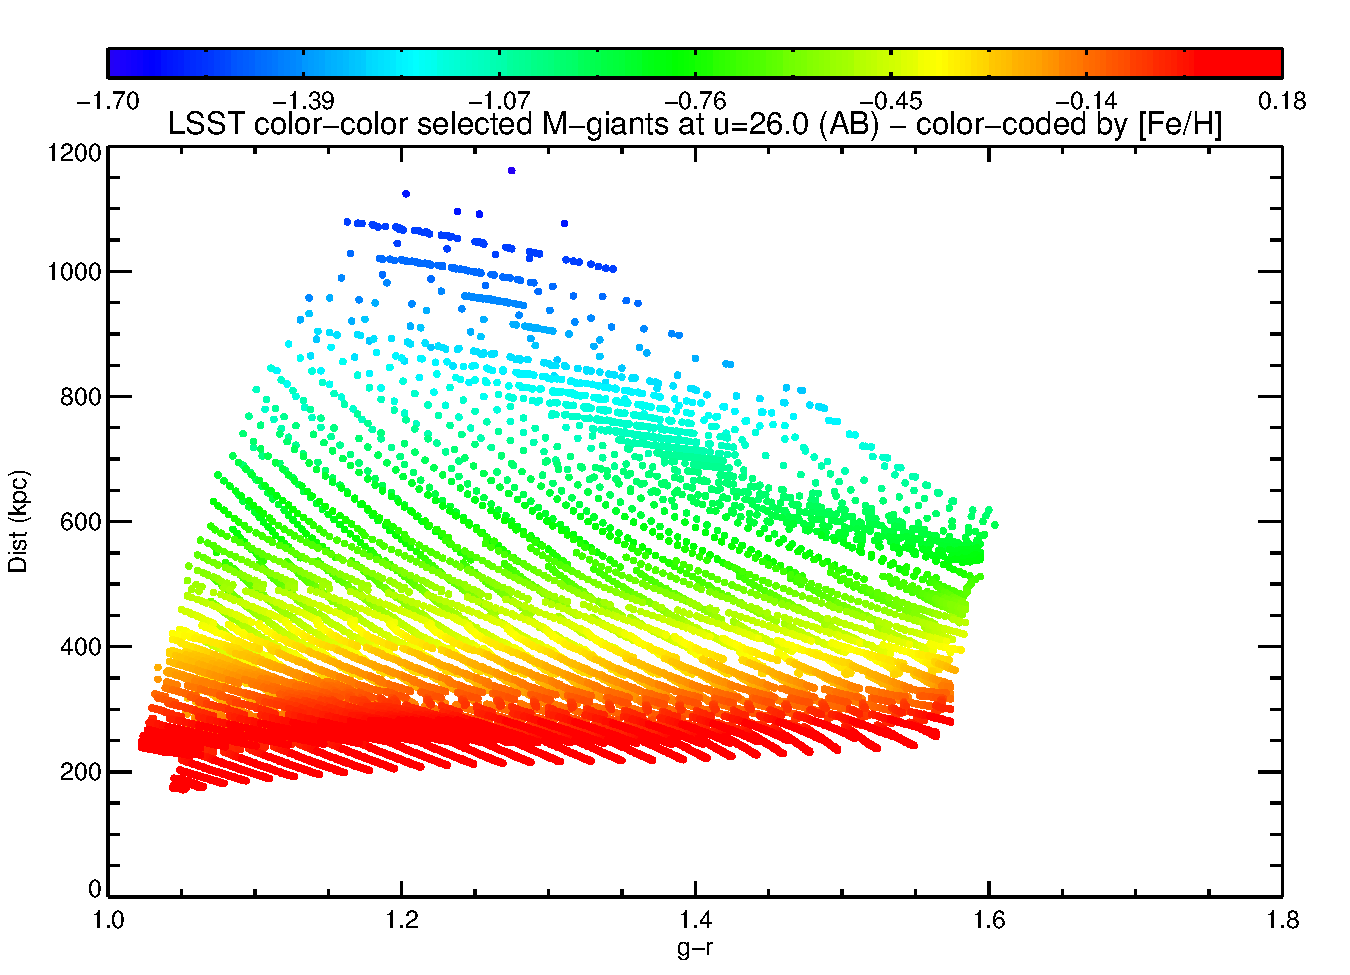
\includegraphics[scale=0.5]{./figs/milkyway/lsst_mgiants_grdist.pdf}
  \caption{Distance to which red giant stars can be identified in the galactic halo asuuming a limiting magnitude
  of u=26.0. The color code scales with the metallicity of the stars. More metal-poor stars can be 
  detected to farther distances. \label{fig-MW-giants}}
\end{center}
\end{figure}


% --------------------------------------------------------------------

\subsection{Metrics}
\label{sec:\secname:MW_Halo_metrics}

\textbf{Star-Galaxy Separation:} For main sequence stars, the useful depth of
the survey will likely not be the photometric detection limit but will instead
be set by the ability to differentiate stars from unresolved background
galaxies. Towards faint magnitudes the contamination by galaxies worsens
significantly for several reasons: the number of galaxies is rising
substantially, the angular size of galaxies is shrinking, and our ability to
distinguish stars from marginally resolved galaxies diminishes for faint
sources simply due to photon statistics. While the fundamental properties of
the contaminant sources is beyond our control, our ability to reject these
sources depends on survey parameters such as the distribution of seeing across
visits and the depth of these visits.

We are currently in the process of developing a metric that will estimate our
ability to separate stars and galaxies for any observation depth and seeing
conditions. This requires both an understanding of how images of a source are
measured and classified as either a star or galaxy, and how the population of
stars and galaxies vary in number and size (for galaxies) with depth. Our model
uses the distribution of galaxies in size and number, derived from HST COSMOS
observations, along with a fully Bayesian model decision formalism to compute
the expected completeness and contamination in star-galaxy separation.
Computationally for each position in the survey footprint we interpolate the
results from that work on a grid in seeing, galaxy size, and coadd depth, then
integrate over the distribution of galaxy sizes. This modeling process is
currently being verified against existing surveys, and will be incorporated into
the observing strategy study at a later date.

\textbf{Distance to the farthest RR Lyrae stars:} This metrics involves the ability to
recover an RR Lyrae star as a function of its distance. An RR Lyrae star may be
considered as recovered if its period and amplitude are within 10\% of their real values.
The distance is calculated using the mean magnitude of the recovered RR Lyrae stars 
(in the more IR photometrics bands) and the interstellar extinction (maps are available 
now in MAF).  Output of this metric is the distance at which certain percentage of RR 
Lyrae stars (eg. 80\%) can be recovered by LSST. It is expected that the results 
of this metric at low galactic latitudes will be largely dependent on the chosen observational 
strategy. 

A reasonable Figure of Merit for this sub-project is the volume of the halo within RR Lyrae stars 
can be recovered. Similarly, another Figure of Merit is the fraction of the Galactic thick disk's volume that can be 
traced by RR Lyrae stars.

\textbf{Distance to the farthest main sequence stars and giant stars:} Being non-variable objects
the metrics for these objects are somewhat simpler and requires the determination of the limiting
magnitude (in u band) for which galaxy/star separation is reliable to certain level. Then, a figure of
merit is the volume of the halo mapped with these tracers. 



% --------------------------------------------------------------------

\subsection{OpSim Analysis}
\label{sec:\secname:MW_Halo_analysis}

Table \ref{tab_SummaryMWHalo} summarizes the science Figures of Merit
for the Milky Way Halo science cases for LSST. OpSim analysis for this
Section will be summarized in that Table; at the present date (April
2016) placeholder rows are given for the FoM's. Input from the readers
is welcome!

%%% SUMMARY TABLE FOR THIS SUBSECTION

\begin{table}
  \begin{tabular}{l|p{6cm}|c|c|c|c|p{5cm}}
    FoM & Brief description & {\rotatebox{90}{\opsimdbref{db:baseCadence} }} & {\rotatebox{90}{\opsimdbref{db:opstwoPS} }} & {\rotatebox{90}{future run 1}} &  {\rotatebox{90}{future run 2}} & Notes \\
    \hline
    1.1. & \footnotesize{Survey volume to RR Lyraes}      & - & - & - & - & \footnotesize{Volume within which the distance to a template RR Lyrae star can be estimated to 10\% uncertainty.} \\
    1.2. & \footnotesize{Survey volume to Main Sequence tracers} & - & - & - & - & \footnotesize{(Including star-galaxy separation)} \\
    1.3. & \footnotesize{Survey volume to Red Giants} & - & - & - & - & - \\
%    2.1. & \footnotesize{Completeness of metallicity sub-structure recovery as a function of distance} & - & - & - & - & \footnotesize{Over all three tracer populations?} \\ 
%    3.1. & \footnotesize{Uncertainty and bias in age distribution parameterization of the main Halo population} & - & - & - & - & - \\
%    3.2. & \footnotesize{Uncertainty and bias in the population fraction identified correctly with each halo component} & - & - & - & - & \footnotesize{Some overlap with Halo astrometry FoM?} \\
\end{tabular}
\caption{Summary of figures-of-merit (FoMs) for the Galactic Halo science cases. The best value of each FoM is indicated in bold. Runs \opsimdbref{db:baseCadence} and \opsimdbref{db:opstwoPS} refer to the Baseline and PanSTARRS-like strategies, respectively. See Section \ref{sec:MW_Halo}.}
\label{tab_SummaryMWHalo}
\end{table}


% --------------------------------------------------------------------

%\subsection{Discussion}
%\label{sec:\secname:MW_Halo_discussion}

%Discussion: what risks have been identified? What suggestions could be
%made to improve this science project's figure of merit, and mitigate
%the identified risks?


% ====================================================================

\navigationbar

% ====================================================================
%+
% SECTION:
%    section-name.tex  % eg lenstimedelays.tex
%
% CHAPTER:
%    chapter.tex  % eg cosmology.tex
%
% ELEVATOR PITCH:
%    Explain in a few sentences what the relevant discovery or
%    measurement is going to be discussed, and what will be important
%    about it. This is for the browsing reader to get a quick feel
%    for what this section is about.
%
% COMMENTS:
%
%
% BUGS:
%
%
% AUTHORS:
%    Phil Marshall (@drphilmarshall)  - put your name and GitHub username here!
%-
% ====================================================================

\section{Mapping the Milky Way Disk}
\def\secname{MW_Disk}\label{sec:\secname} % For example, replace "keyword" with "lenstimedelays"

\noindent{\it Will Clarkson, Peregrine McGehee, Jay Strader, Chris Britt}  % (Writing team)

% This individual section will need to describe the particular
% discoveries and measurements that are being targeted in this section's
% science case. It will be helpful to think of a ``science case" as a
% ``science project" that the authors {\it actually plan to do}. Then,
% the sections can follow the tried and tested format of an observing
% proposal: a brief description of the investigation, with references,
% followed by a technical feasibility piece. This latter part will need
% to be quantified using the MAF framework, via a set of metrics that
% need to be computed for any given observing strategy to quantify its
% impact on the described science case. Ideally, these metrics would be
% combined in a well-motivated figure of merit. The section can conclude
% with a discussion of any risks that have been identified, and how
% these could be mitigated.

%A short preamble goes here. What's the context for this science
%project? Where does it fit in the big picture?

Many populations of great importance to Astronomy exist predominantly
in or near the Galactic Plane, and yet are sufficiently
sparsely-distributed (and/or faint enough) that LSST is likely to be
the only facility in the forseeable future that will be able to
identify a statistically meaningful sample. Some (such as the novae
that allow detailed study of the route to Type Ia Supernovae) offer
unique laboratories to study processes of fundamental importance to
astrophysics at all scales. Others (like intra-disk microlensing
events) offer the {\it only} probe of important populations. An
important collateral benefit of studies in the plane with an LSST-like
facility, is improved mapping of the distribution and observational
effects of the ISM (particularly dust), which is of importance to all
IR/Optical/UV observational studies.

% --------------------------------------------------------------------

\subsection{Target measurements and discoveries}
\label{sec:\secname:MW_Disk_targets}

%Describe the discoveries and measurements you want to make.

%Now, describe their response to the observing strategy. Qualitatively,
%how will the science project be affected by the observing schedule and
%conditions? In broad terms, how would we expect the observing strategy
%to be optimized for this science?

We have identified five science cases within the general area of Milky
Way Disk studies, that will have a diversity of dependencies on
observing strategy (e.g. slow intrinsic variability vs fast intrinsic
variability vs no variability). When the figures of merit have been
computed for these science cases, the results will be summarized in a Table in Section~\ref{sec:\secname:MW_Disk_discussion}.

\begin{itemize}
  \item 1. Quantifying the large quiescent compact binary population via variability;
  \item 2. New insights into the behavior of Novae and the route to Type Ia Superovae;
  \item 3. The next Galactic Supernova;
  \item 4. Measuring population parameters of planets outside the Snow Line with Microlensing;
  \item 5. A three-dimensional Dust map and improvements in the reddening law
\end{itemize}

Motivation and qualitative description of response to observing strategy:

{\bf 1. Probing quiescent compact binaries via variability:} Of the
millions of stellar-mass black holes formed through the collapse of
massive stars over the lifetime of the Milky Way, only $\sim 20$ have
been dynamically confirmed through spectroscopic measurements (e.g.,
Corral-Santana et al.~2015). Many questions central to modern
astrophysics can only be answered by enlarging this sample: which
stars produce neutron stars and which black holes; whether there is a
true gap in mass between neutron stars and black holes; whether
supernova explosions result in large black hole kicks. 

There is expected to be a large population of black hole binaries in quiescence
with low X-ray luminosities from $\sim 10^{30}$--$10^{33}$ erg/s.
Such systems can be identified as optical variables that show unique,
double-humped ellipsoidal variations of typical amplitude $\sim 0.2$
mag due to the tidal deformation of the secondary star, which can be a
giant or main sequence star. In some cases analysis of the light curve
alone can point to a high mass ratio between the components,
suggesting a black hole primary; in other cases the accretion disk
will make a large contribution to the optical light which results in
intrinsic, random, and fast variations in the light curve. The disk
contribution to optical light can change over time, and several years
of data is necessary to properly subtract the accretion disk
contribution in order to properly fit ellipsoidal veriations (Cantrell
et al. 2010). The brighter sources will be amenable to spectroscopy
with the current generation of 4-m to 10-m telescopes to dynamically
confirm new black holes; spectroscopy of all candidates should be
possible with the forthcoming generation of large telescopes. Thus,
LSST would trigger a rich variety of observational investigations of
the accretion/outflow process through studies of this large, dark
population.

While we have focused above on black hole binaries, we note that LSST
would be crucial for investigations of neutron star and white dwarf
binaries. For example, the total number of compact binaries 
is presently
poorly understood---Population models of neutron star X-ray binaries diverge by orders 
of magnitude, largely due to uncertainties in the common envelope phase of binary evolution (e.g. Pfahl et al, 2003; Kiel \& Hurley, 2006; van Haaften et al, 2015). This is
poorly constrained but has a large impact on, for example, LIGO event
rates. A simple test case of common envelope evolution is available in the number of dwarf novae (DNe) 
(accretion disk instability outbursts around white dwarfs), a population that does not suffer from
some of the complicating factors that neutron star and black hole binaries do (e.g. supernova kicks). 
Theoretical estimates routinely yield a significantly higher number of DNe than are observed in the solar
neighborhood. Understanding the true specific frequency of these
systems provides a key check on common envelope evolution.  LSST will detect dwarf novae, which last at least several days
with typical amplitudes of 4--6 mag,
out to kpc scales. This will allow a test of not only the number of
cataclysmic variables, but also of the 3D distribution within the
Galaxy and dependence on metallicity gradients (Britt et al. 2015).

{\it Response to observing strategy:} Since most black hole candidates
have been identified near the plane in the inner Milky Way (68\%, 92\%
within $5^{\circ}, 10^{\circ}$~of the Plane), this science case {\it
    requires} that LSST observe the plane with sufficient cadence to
  detect the $\sim$hundreds of quiescent black-hole binaries by virtue
  of their variability. The natural choice for a survey for
  low-luminosity black hole binaries would be to extend the
  Wide-Fast-Deep survey throughout the Plane in the direction of the
  inner Milky Way. The orbital period of these systems is short (typically $<1$ day), so that a rolling cadence
  for at least parts of the Plane should be considered. For dwarf novae, the cadence of observations
  is critical in obtaining an accurate measure of the population of
  cataclysmic variables, as a long baseline is necessary to recover
  low duty cycle systems while widely-space observations
 would miss short outbursts.

%Describe the discoveries and measurements you want to make.

%Now, describe their response to the observing strategy. Qualitatively,
%how will the science project be affected by the observing schedule and
%conditions? In broad terms, how would we expect the observing strategy
%to be optimized for this science?

{\bf 2. Novae and the route to Type Ia Supernovae:} Only $\sim 15$
novae (explosions on the surfaces of white dwarfs) are discovered in
the Milky Way each year, while observations of external galaxies show
that the rate should be a factor of $\sim 3$ higher (Shafter et
al.~2014). Evidently, we are missing 50--75\% of novae due to their
location in crowded, extinguished regions, where they are not bright
enough to be discovered at the magnitude limits of existing transient
surveys. Fundamental facts about novae are unknown: how much mass is
ejected in typical explosions; whether white dwarfs undergoing novae
typically gain or lose mass; whether the binary companion is important
in shaping the observed properties of nova explosions. Novae can serve
as scaled-down models of supernova explosions that can be tested in
detail, e.g., in the interaction of the explosion with circumstellar
material (e.g., Chomiuk et al.~2015). Further, since accreting white
dwarfs are prime candidates as progenitors of Type Ia supernovae, only
detailed study of novae can reveal whether particular systems are
increasing toward the Chandrasekhar mass as necessary in this
scenario.

{\it Response to observing strategy:} Most novae occur in the Galactic
Plane and Bulge, and therefore the inclusion of the Plane in a survey
of sufficient cadence to find these events promptly is of paramount
importance for this science. These events will trigger
multi-wavelength follow-up ranging from the radio to X-ray and
$\gamma$-rays; these data are necessary for accurate measurements of
the ejected mass.

{\bf 3. The First Galactic Supernova:} A supernova in the Milky Way
would be among the most important astronomical events of our lifetime,
with enormous impacts on stellar astrophysics, compact objects,
nucleosynthesis, and neutrino and gravitational wave astronomy. The
estimated rate of supernovae (both core-collapse and Type Ia) in the
Milky Way is about 1 per 20--25 years (Adams et al.~2013); hence there
is a 40--50\% chance that this would occur during the 10-year LSST
survey. If fortunate, such an event will be located relatively close
to the Sun and will be an easily observed (perhaps even naked-eye)
event. However, we must be cognizant of the likelihood that the
supernova could go off in the mid-Plane close to the Galactic Center
or on the other side of the Milky Way---both regions covered by
LSST. While any core-collapse event will produce a substantial
neutrino flux, alerting us to its existence, such observations will
not offer precise spatial localization. The models of Adams et
al.~(2013) indicate that LSST is the \emph{only} planned facility that
can offer an optical transient alert of nearly all Galactic
supernovae. 

{\it Response to observing strategy:} Even if the supernova is not too
faint, LSST will likely be the sole facility with synoptic
observations preceding the explosion, providing essential photometric
data leading up to the event---but only if LSST covers the Plane at a
frequent cadence. Just {\it how} frequent is open to exploration at
present, but the prospect of high-sensitivity observations of the
location of such a supernova {\it before} it takes place are clearly
of enormous scientific value. A secondary issue is the prospect that
an easily-observed Milky Way supernova might be too bright for LSST to
measure precisely with its planned exposure time, with a roughly 82\%
chance of a core-collapse supernova reaching one or two magnitudes
brighter than LSST's nominal saturation limit (with a 1/3 chance that
a ccSN would reach $m_V \sim 5$~(Adams et al. 2013). For a Type Ia in
the Milky Way, Adams et al. (2013) estimate $m_{V, max} \lesssim
13.5$~in 92\% of cases.

{\bf 4. Population parameters of planets beyond the Snow Line with Microlensing:} Gould
(2013) shows that LSST could be an effective intra-disk microlensing
survey (in which disk stars are lensed by other objects in the disk,
such as exoplanets, brown dwarfs, or compact objects). The lower
stellar density compared to past bulge-focused microlensing surveys
would be offset by the larger area covered by LSST. The predicted rate
of high magnification microlensing events that are very sensitive to
planets would be $\sim 25$ per year. This survey would be able to
detect planets at moderate distances from their host stars, a regime
poorly probed by standard Doppler and transit techniques. The LSST
data alone would not be sufficient: the detection of a slow ($\sim$
days) timescale increase in brightness of a disk star would need to
trigger intensive photometric observations from small (1-m to 2-m
class) telescopes that would observe at high cadence for the 1--2
months of the microlensing event. This would represent an excellent
synergy between LSST and the wider observing community, and would
directly take advantage of the capabilities unique to LSST.

{\it Response to observing strategy:} To catch lensing events as they
start to brighten, with sufficient fidelity to trigger the intensive
follow-up required, the models of Gould (2013) suggest each field
should be observed once every few nights. With sparser coverage,
the survey would lose sensitivity to microlensing events in progress.

{\bf 5. Dust in the Milky Way disk:} The Pan-STARRS1 survey (PS1) has
produced a three-dimensional dust map of the region of the sky covered
in their 3$\pi$ survey (which excludes a large part of the Galactic
Plane toward the south). Such maps are necessary to accurately measure
the intrinsic luminosities and colors of both Galactic and
extragalactic sources. The PS1 map (Schlafly et al.~2014) saturates at
extinctions $E(B-V) > 1.5$ as their tracer stars fall out of the
survey catalogs fainter than $g\sim 22$, meaning that this
high-fidelity map does not extend uniformly to within a few degrees of
the midplane. In addition, it only extends to a distance of about 4.5
kpc. Deep LSST data will allow this map to be extended to much higher
extinctions and larger distances. Owing to the high extinction and the
use of blue filters, this project is less affected by crowding than
other projects requiring photometry in the Plane. 

{\it Response to observing strategy:} When focusing on dust in the ISM (as
opposed to time-domain studies, e.g., dust around star-forming
regions or young stars), the main drivers of feasibility are
coverage of the few degrees around the Plane with sufficient photometric depth
and accuracy. This project is less affected by crowding than other
projects requiring photometry in the Plane owing to its use of blue
filters and the high extinction.  Nonetheless, quantiative estimates of
the expected photometric accuracy in coadded $u$ and $g$ images at low
Galactic latitude are desirable.


% --------------------------------------------------------------------

\subsection{Figures of Merit}
\label{sec:\secname:MW_Disk_metrics}

%Quantifying the response via MAF metrics: definition of the metrics,
%and any derived overall figure of merit.

Unpolished notes about likely (reasonably straightforward) figures of
merit (FoM) follow, along with (in some cases) possible directions for
future higher-level FoM. In many cases, dependencies on
Metrics are identified.  \new{WIC - Note to co-authors: these FoM
  were chosen to build off existing metrics in development. To take
  one example, Peter Y has developed some nice ipython Notebooks that
  illustrate representative Monte Carlo tests for periodicity
  detection including spatial variation - thus I think the Figures of Merit
  below should be straightforward to implement by modification of
  existing tools.}


{\bf FoM 1.1 - Fraction of quiescent
  black hole binaries detectable through ellipsoidal variability, as a function of location on sky and distance.}
Dependencies:
\begin{itemize}
  \item Monte Carlo in period, phase and shape parameters (ASCII input?) for variables as measured in a particular OpSim run. Likely run Monte Carlo for a representative number (ten?) of well-chosen orbital periods within the 0.1-5d range;
  \item (Since these are short-period objects): the ``PeriodicMetric'' of Lund et al. (2015);
  \item Will likely need reasonably high-spatial-resolution HEALPIX slices and a prescription for population density as a function of position on-sky (can be analytic).
\end{itemize}
Possible higher-order FoM: errors on the population size (mass
function??) derived from a survey under a given observing
strategy. Can imagine just adding up the ``recovered'' qLMXB
population and comparing it to that simulated. Some white noise componant of varying strengths could be
added to the light curves to simulate various contributions of the accretion disk to the continuum light. 
Note that the survey will necessarily be highly incomplete (inclination effects, etc.), it
is the likely {\it uncertainty} on the completeness-correction that
would be crucial in this case. 

{\bf FoM 1.2 - Fraction of dwarf novae detected in a given survey
  run as a function of location and distance.}
Dependencies:
\begin{itemize}
  \item Monte Carlo in distribution of maximum brightness and rise/decay timescale;
    \item "Triples" without filter constraints (given a prior detection in each filter)- what fraction are recovered?
    \item Histogram of duty cycle recovery efficiency versus duration of outburst and recurrence time.
    \item Histogram of recovery efficiency of maximum brightness of dwarf nova versus duration and recurrence time (if assume subsequent outbursts have similar profiles).
    \end{itemize}
Higher-level FoM: Uncertainty in LIGO event rates due to
uncertainties in common envelope evolution, which drives uncertainties in both LIGO event rates and DN population.

{\bf FoM 2.1 - Fraction of identified Novae as a function of location on-sky, distance, and time since initial rise.}
Dependencies:
\begin{itemize}
  \item Is the ``Triplets'' metric sufficient (i.e. is this ``just'' a case of supplying the metric the correct $\Delta t$~parameter values)?;
    \item What is the maximum interval since initial rise that would be acceptable? (Is this a function of waveband for followup?)
\end{itemize}
Possible higher-order FoM: error on inferred rate of Type Ia supernovae?

%{\bf FoM 3.1 - Maximum time-interval {\it before} triggering of a SN in the Milky Way that LSST would h%ave taken precursor data.}
%Dependencies:
%\begin{itemize}
%  \item This FoM would probably be very easy to calculate (just estimate the mean time between observat%ions). However the acceptable limits still need thought:
%  \item How many colors are sufficient? Any observations at all before the SN goes off, or would a comp%lete set in all filters be needed to characterize the candidate progenitor?
%    \item What level of variability sensitivity is really needed? Would just an extremely deep image of% the SN field before the event be sufficient?
%\end{itemize}
%{\bf FoM 3.2 - Maximum time-interval {\it after} the SN event for triggering followup.}
%Dependencies:
%\begin{itemize}
%  \item Similar to FoM 3.1. 
%    \item Is it important to know the discovery space for LSST? If a
%      supernova at $m_V~15$~goes off, other facilities are likely to
%      spot it...
%\end{itemize}


\new{\bf FoM 3.1 - Fraction of Galactic supernovae for which LSST would detect variability {\it before} the main Supernova event. Dependencies:}
\begin{itemize}
  \item \new{Assume the probability of a SN going off scales with the number of stars along the line of sight to some depth. The ``starcount'' metric in sims-maf-contrib (by Mike Lund and collaborators) calculates this value out to some fiducial distance. Additionally}; 
\item \new{This FoM requires an assessment of the ability of LSST to detect a particular lightcurve shape. Several options are possible at this time; we have selected ``metrics.TransientMetric'' from the baseline lsst-sims. Therefore also};
\item \new{a lightcurve shape for the pre-SN variability must be assumed.}
\end{itemize}

% WIC - removed this one since it's a bit low-level...
%
%{\bf FoM 3.2 - Maximum time-interval {\it after} the SN event for triggering followup.}
%Dependencies:
%\begin{itemize}
%  \item Similar to FoM 3.1. 
%    \item Is it important to know the discovery space for LSST? If a
%      supernova at $m_V~15$~goes off, other facilities are likely to
%      spot it...
%\end{itemize}



{\bf FoM 4.1 - Fraction of accurately-triggered Microlens candidates as a function of location, distance, lens mass.}
Dependencies:
\begin{itemize}
  \item Analytic (?) model for microlens lightcurve for representative sample of microlens parameters;
    \item transientASCIIMetric may well already do what we need! 
\end{itemize}

{\bf FoM 4.2 - errors in the (mass function, distance distribution) of intra-disk microlensed planets.}
Dependencies:
\begin{itemize}
  \item Event rate with sufficient-cadence observations to trigger followup as a function of (distance, lens mass);
\end{itemize}

{\bf FoM 5.1 - Errors in derived $E(B-V)$, $n_H$~as a function of
  location in the Plane.}
Dependencies:
\begin{itemize}
  \item SNR scaling with apparent magnitude
    \item For the M dwarf based technique, the relation between
      reddening-invariant index $[Q_{gri}]$~and intrinsic $g-i$~are
      expressed as polynomials, so expect non-linear relation with
      photometric error.  
      \item This uses a 5th-order polynomial to describe the
        $(Q_{gri}, g-i)$~stellar locus for M dwarfs $(g-i > 1.6)$.
        \item Care must be taken to correctly propagate errors through
          the various indices used - not trivial with so many choices
          of flux ratio used.
          \item Uncertainties in the parameterizations used for e.g. color-$M_V$~relationships.
            \item The above are all for every location probed on the map.
\end{itemize}



% --------------------------------------------------------------------

\subsection{OpSim Analysis}
\label{sec:\secname:MW_Disk_analysis}

\new{(To stimulate input from collaborators, we have implemented a mock-up of a simple figure of merit for the Galactic Supernova case. We choose FoM 3.1 - the fraction of galactic supernovae for which an SN2010mc-like pre-SN outburst could be discovered by LSST. The results of all FoM's for this Section are collected in Table \ref{tab_SummarMWDisk}.)}

\new{{\bf FoM 3.1: Fraction of Galactic supernovae for which LSST would detect variability {\it before} the main Supernova brightening:}}
\begin{itemize}
\item \new{{\it Definition:} 
\begin{equation}
  FoM_{preSN} \equiv \frac{ \sum^{sightlines}_{i} f_{var, i} N_{\ast, i} } {\sum^{sightlines}_{i} N_{ast, i}}
\end{equation}
where $f_{var, i}$~is the fraction of transient events that LSST would detect for observing strategy including the $i$'th sightline, $N_{\ast,i}$~the number of stars present along the $i$'th sightline, and the FoM is normalized by the total number of stars returned by the density model over all sightlines. (For the two OpSim runs tested here, enigma-1189 and ops2-1092, the normalization factors differ by $\sim 0.1\%$.) Therefore $0.0 \le FoM_{preSN} \le 1.0$.}
\item \new{{\it Assumptions (observational):} Pre-SN variability similar to the pre-SN outburst of SN2010mc (Ofek et al. Nature). The pre-SN variability is modeled as a sawtooth lightcurve (in apparent magnitude). We assume this transient event will always reach brightness sufficient for LSST to observe, so opt for a very bright peak apparent magnitude in all filters. We assume that the probability of a supernova going off is proportional to the number of stars along a particular line of sight.}
\item \new{{\it Parameters used:} The pre-SN outburst is simulated using the lsst-sims metrics.TransientMetric module. The lightcurve used has the following parameters: rise slope $-2.4$; time to peak; $20$~days; decline slope: $0.08$; total transient duration: 80 days. All filters are used in the detections, and 20 evenly-spaced phases are simulated for sensitivity to pathological cases (parameter nPhaseCheck=20). Peak apparent magnitudes used: $\{ 11,9,8,7,6,6\}$~in $\{u,g,r,i,z,y\}$. Then, $f_{var, i}$~is taken as the ``Sawtooth Alert'' quantity returned by metrics.TransientMetric. The starcounts metric (in sims-maf-contrib) is used to estimate the number of stars along a given line of sight, using fiducial distance limits ($10$pc $\le d \le 80$kpc).}
\item \new{{\it \bf Results:} $FoM_{preSN}$(enigma-1189) = 0.251, while $FoM_{preSN}$(ops2-1092)=0.852. See Figure \ref{f_opSim_GalacticSN} for a breakdown of this figure of merit across sightlines.}

\end{itemize}
\begin{figure}
\begin{center}
  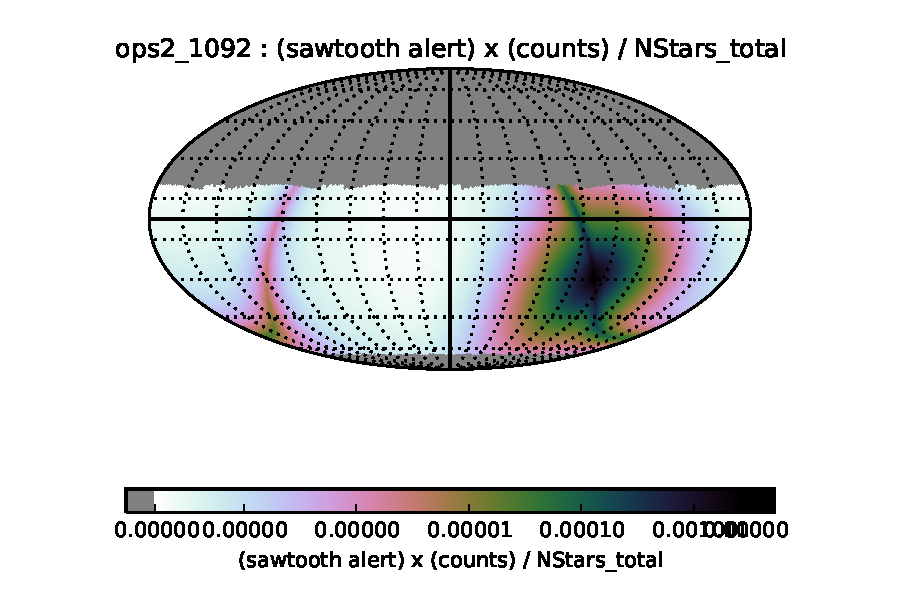
\includegraphics[width=7cm]{./figs/milkyway/galacticSN_SkyMap_1092.pdf}
  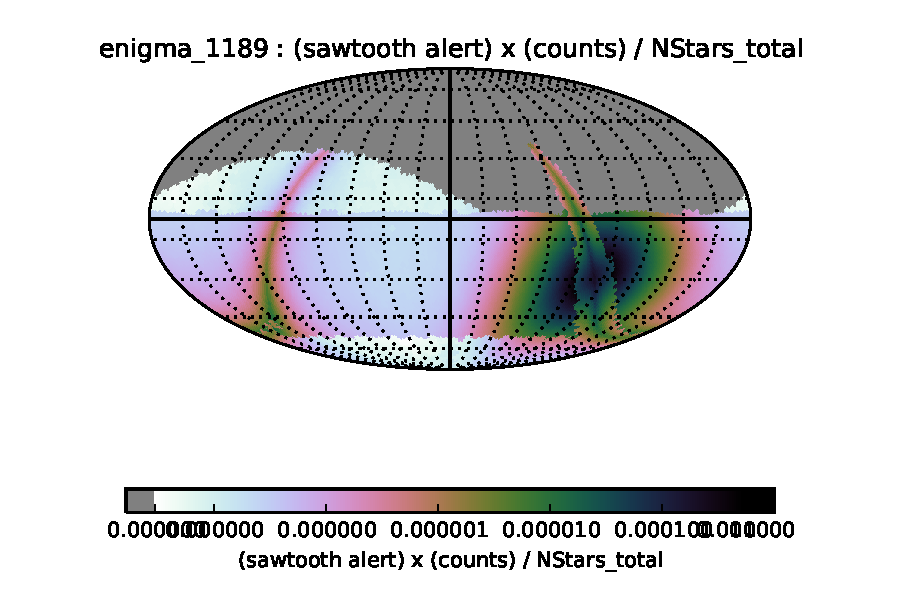
\includegraphics[width=7cm]{./figs/milkyway/galacticSN_SkyMap_1189.pdf}
%  \includegraphics[width=6cm]{./figs/milkyway/galacticSN_Histogram_1092.pdf}
%  \includegraphics[width=6cm]{./figs/milkyway/galacticSN_Histogram_1189.pdf} 
  \caption{\new{Figure of merit $FoM_{preSN}$~describing LSST's sensitivity to any pre-Supernova outburst, broken down by sightline, as sky-maps. $FoM_{preSN}$~is estimated for two OpSim runs (to-date); ops2-1092 (left) and enigma-1189 (right). The normalizing factors $N_{\ast, total}$ are $1.120\times 10^{12}$~for ops2-1092 and $1.121 \times 10^{12}$~for enigma-1189. The imprint of reduced sampling towards the inner plane can be clearly seen for enigma-1189.}}
\end{center}
\label{f_opSim_GalacticSN}
\end{figure}


%The current baseline cadence (${\tt enigma\_1189}$) partially excludes the Galactic Plane from the% deep-wide-fast survey and instead adopts a 
%nominal 30 visits per filter as part of a special proposal. We have proposed an OpSim run that inc%ludes the Galactic Plane in the 
%deep-wide-fast survey:

%\url{https://github.com/LSSTScienceCollaborations/ObservingStrategy/blob/master/opsim/Proposal_GP.md}

% The Figures of Merit listed above must now be implemented and applied to the OpSim databases.

%The metrics listed above should be carefully compared between our proposed run and the baseline cadence.


% --------------------------------------------------------------------

\subsection{Discussion: required work}
\label{sec:\secname:MW_Disk_discussion}

The Figures of Merit listed above must now be implemented within the
sims\_maf framework and applied to representative science
cases. \new{See Table \ref{tab_SummaryMWDisk} at the end of this subsection for initial
  efforts along these lines.}

We welcome input and volunteers for this effort. 

Qualitatively, however, we can note immediately that the current
baseline cadence (${\tt enigma\_1189}$) partially excludes the
Galactic Plane from the deep-wide-fast survey and instead adopts a
nominal 30 visits per filter as part of a special proposal - which
also tends to cluster the visits in the inner Plane within the first
few years of the survey. This already seriously compromises the time
baseline (see figure 4.3 of Section
\ref{sec:MW_Astrometry:MW_Astrometry_OpSim} for a demonstration applied to
proper motions).

We have proposed an OpSim run that includes the Galactic Plane in the
deep-wide-fast survey:

\url{https://github.com/LSSTScienceCollaborations/ObservingStrategy/blob/master/opsim/Proposal_GP.md}

\begin{table}
  \begin{tabular}{l|p{6cm}|c|c|c|c|p{5cm}}
    FoM & Brief description & {\rotatebox{90}{enigma-1189}} & {\rotatebox{90}{ops2-1092}} & {\rotatebox{90}{future run 1}} &  {\rotatebox{90}{future run 2}} & Notes \\
    \hline
    1.1 & \footnotesize{LMXB ellipsoidal variations}      & - & - & - & - & - \\
    1.2 & \footnotesize{Uncertainty in dwarf nova duty cycle}   & - & - & - & - &  \footnotesize{LSST as initial trigger} \\
    2.1 & \footnotesize{Fraction of Novae detected}       & - & - & - & - &  - \\
    3.1 & \footnotesize{Galactic Supernova pre-variability} & 0.25 & {\bf 0.85} & - & - & \footnotesize{Fraction of SN2010mc-like outbursts that LSST would detect; $FoM_{preSN} = f_{var} \times N_{\ast}$} \\
    4.1 & \footnotesize{Fraction of triggered microlens candidates} & - & - & - & - & - \\
    4.2 & \footnotesize{Uncertainty in disk-disk microlens distribution parameters due to missed events} & - & - & - & - & \footnotesize{LSST as initial microlens trigger} \\
    5.1a & \footnotesize{Median (over sight-lines) of the uncertainty in $E(B-V)$} & - & - & - & - & \footnotesize{(Most useful FoM probably a spatial map of the uncertainty.)} \\
    5.1b & \footnotesize{Variance (over sight-lines) of the uncertainty in $E(B-V)$} & - & - & - & - & - \\
  \end{tabular}
\caption{Summary of figures-of-merit for the Galactic Disk science cases. The best value of each FoM is indicated in bold.}
\label{tab_SummaryMWDisk}
\end{table}


%Discussion: what risks have been identified? What suggestions could be
%made to improve this science project's figure of merit, and mitigate
%the identified risks?



% ====================================================================

\navigationbar

% ====================================================================
%+
% SECTION:
%    MW_Astrometry.tex
%
% CHAPTER:
%    galaxy.tex
%
% ELEVATOR PITCH:
%
%-
% ====================================================================

\section{Astrometry with LSST: Positions, Proper Motions, and Parallax}
\def\secname{MW_Astrometry}\label{sec:\secname}

\credit{dgmonet}, \credit{DanaCD}, \credit{jgizis}, \credit{mliu},
\credit{caprastro}, \credit{willclarkson}, \credit{yoachim}

A number of Milky Way science cases of interest to the Astronomical
community will depend critically on the astrometric accuracy LSST will
deliver. While ``astrometry'' is not a science case in the framework
of this white paper, LSST's astrometric performance will be sensitive
to the particular choice of observing strategy.
%While astrometry is not a science case, high astrometric accuracy enables
%a large number of science cases.
Hence, the LSST Observing Strategy needs to be examined for systematic
trends that might limit or even preclude precise measures of
stellar positions, proper motions, parallaxes, and perturbations that
arise from unseen companions.

\autoref{sec:\secname:MW_Astrometry_measurements} highlights two
science cases at opposite scales of distance from the Sun that require
accurate and precise astrometry and/or proper motion
measurements. \autoref{sec:\secname:MW_Astrometry_metrics} presents
Metrics for LSST's astrometric performance, and discusses Figures of
Merit for the two highlighted science cases. These metrics are applied to two example OpSim runs in
\autoref{sec:\secname:MW_Astrometry_OpSim}. Finally in Section
\ref{sec:\secname:MW_Astrometry_furtherwork}, the work that is still
needed is discussed, both in terms of the Metrics and the Figures of
Merit that depend on them.

%Each of these cases stresses different aspects of the LSST hardware, software,and observing strategies.

%, here we highlight three representative science cases.
%that illustrate the various impacts of the observing strategy might
%be:
%To highlight the
%various astrometric impacts of the strategy, three science cases have
%been chosen for particular attention:

%\subsection{Introduction: Astrometry as a special case}
%\label{sec:\secname:MW_Astrometry_intro}

\subsection{Target Measurements and Discoveries}
\label{sec:\secname:MW_Astrometry_measurements}

%\begin{itemize}
%\item[1.] Identification of Streams in the Galactic Halo using proper motions.
%\item[2.] A complete sample of stars in the solar neighborhood.
%\end{itemize}
%\item The tie between the Radio and Optical realizations of the International Celestial Reference System.
%\item The specific and ensemble agreement between LSST and Gaia parallaxes.

{\bf 1. Identification of Streams in the Galactic Halo Using Proper Motions}

Much of the Milky Way's stellar halo was built by the accretion of smaller galaxies. Given that these galaxies
were generally of low mass, their tidal debris should still form coherent structures in phase space, especially
in the outer Galaxy where dynamical times are long. The identification of these streams would allow
a reconstruction of the accretion history of the Milky Way. Tides also lead to the dissolution of globular clusters,
leaving notably thin streams that serve as sensitive tracers both of the Galactic potential and of the presence of dark
subhalos.

A relatively small number of streams, originating from both dwarfs and globular clusters, have been identified via photometry
of individual stars in large surveys such as SDSS\@. However, only the highest surface brightness structures can be found
in this manner, and it is often difficult to trace the streams over their full extent. LSST will enable streams to be identified
by stellar proper motions, and combined with targeted follow-up spectroscopy, will yield full 6-D position and velocity measurements suitable for dynamical modeling.
Further, it will allow the discovery of tidal debris that is no longer spatially coherent but which can be unambiguously identified in phase space.

Finally, streams and other kinematically-distinct halo substructure
can be identified and characterized by combining proper motions and
photometry in reduced proper-motion diagrams \citep[e.g.,][]{carlin12},
and by analyzing proper-motions of tracers such as
RR Lyrae and giants over large portions of the sky \citep[e.g.,][]{casettidinescu15}.

{\it Response to observing strategy:} Most stars in streams will be main-sequence stars, and the old main sequence turnoff  is located at $r\sim24$ at a distance of 100 kpc.
The nominal LSST proper motion precision at this magnitude is 1 mas yr$^{-1}$, corresponding to about 475 km s$^{-1}$ at this distance. The proper motion
measurements will be better for brighter stars, but in general ensembles of stars will be necessary for accurate measurements. To make accurate proper motion measurements for faint stars, several key components are required. First, a zero point must be established, possibly via background galaxies located in each field. Next, the observations must cover a sufficient range of epochs to reliably detect linear proper motions.

To identify streams over their full lengths of many degrees of the sky, relative astrometry over small fields will not be sufficient. Therefore the absolute astrometric frame is important. Matching the optical astrometry to the radio International Celestial Reference System (ICRS) relies on measuring accurate positions for objects visible in both wavelength regimes.
These are typically distant QSOs. Unfortunately, many QSOs have detectable optical or radio structures that degrade the positions or suggests a displacement between the location of the sources of the radio and optical radiation. LSST will need to identify a large number of point-like QSOs based on their colors and variability.

Since the number of galaxies is overwhelming toward faint magnitudes,
these must be exploited to produce a reliable absolute
proper-motion zero point. By using Gaia stars at the bright end
as absolute proper-motion calibrators we can quantify the precision
and accuracy of background galaxies as a secondary link to an inertial reference system, and thus improve the calibration at the faint end of the survey.

%The tie between the radio and optical reference frames relies on measuring accurate positions for objects visible in both wavelength regimes.  Whereas there are optical variable stars with radio emission, most have associated optical nebulosity that degrades the accuracy of the optical positions. The typical radio+optical object is a QSO.  Unfortunately, many QSOs have detectable optical or radio structures that degrade the positions or suggests a displacement between the location of the sources of the radio and optical radiation.  The major contribution from LSST will be the identification of a large number of QSOs based on their colors that have minimal (if any) spatially extended structure.  The impact of this search has no obvious impact on the cadence other than temporal coverage to identify variability.

{\bf 2. A Complete Sample of Stars in the Solar Neighborhood}

The direct solar neighborhood offers our only chance to get make a complete sample of stars, brown dwarfs, and stellar remnants that encompass the entire formation and dynamical history of the Milky Way. While Gaia will offer parallax measurements for perhaps billions of stars, its faint magnitude limit of $G\sim 20$ will limit its measurements of the lowest-mass objects
and remnants to nearby objects, much less than the thin disk scale height of $\sim 300$ pc. For example, Gaia can only measure parallaxes for $0.2 M_{\odot}$ M dwarfs to about 100 pc
and $0.1 M_{\odot}$ M dwarfs to only \emph{10 pc}, showing that Gaia is ill-suited for studies of the coolest dwarfs. By contrast, LSST can measure parallaxes for $> 10^5$ M dwarfs and thousands of L/T brown dwarfs (the coolest Y dwarfs are too faint even for LSST; little contribution is likely here beyond the sample provided by WISE). Gaia will likewise be limited to cool white dwarfs within $\sim 100$ pc with which to estimate the age of the disk, and the thick disk and halo will be out of reach. LSST can directly compare white dwarf luminosity functions to determine precise differential ages for the thin disk, thick disk, and halo.

{\it Response to observing strategy:} Successfully completing this project will require parallax measurements much fainter than possible with Gaia as well as a verification that the LSST and Gaia parallax measurements are consistent in the overlapping magnitude range.

The measurement of stellar parallax puts the substantial constraints on the observing cadence. There are two major issues: the need to sample a wide range of parallax factor (related to time of year), and breaking the correlation between differential color refraction and parallax factor.

``Parallax factors" characterize the ellipse of the star's apparent motion as seen over the course of a year. The shape of the ellipse is given by the Earth's orbit and is not a free parameter in the astrometric solution. The amplitude of the right ascension parallax factor is close to unity while the amplitude of the declination parallax factor is dominated by the sine of ecliptic latitude.
The right ascension parallax factor has maximum amplitude when the star is approximately six hours from the Sun, so the optimum time for parallax observing is when the
star is on the meridian near evening or morning twilight. Atmospheric refraction displaces the star's apparent position in the direction of the zenith by an amount dependent on both the wavelength of the light and the distance to the zenith. Whereas the measured position of star is a function of the total refraction, the measurement of parallax
and proper motion depends on the differences in the refraction as a function of the color of each star and the circumstances of the observations.  This
dependence is called differential color refraction. The combination of parallax factor and differential color refraction leads to two rules: (i) Observations need to cover the widest possible range in parallax
factor, and (ii) The correlation between parallax factor and hour angle in the observations needs to be minimized.

%with respect to the meanmotion of the reference frame.

%The search for faint proper motion stars has two key components.  The first is the need to identify stars that move from the ensemble of other image features that can cause confusion.  For example, a compact group of stars that contains one or more stars of variable brightness can confuse the catalog correlation algorithm.  The other is the need to establish the zero point. For the case of relative astrometry, meaning the measurement of relative positions in an image, the question remains on how to remove the mean motion of the reference frame.  For example, astrometry on certain classes of galaxies might produce a zero point of sufficient accuracy.  This leads to a third constraint on the observing cadence.
% \begin{itemize}
%\item [3)] Observations must cover a sufficient range of epochs so that stars with
%linear or periodic motions can be identified at a high level of confidence.
%\end{itemize}


%\subsection{Sensitivity of parallax measurements to observing strategy}
%\label{sec:\secname:MW_Astrometry_cadence}

%\medskip


\subsection{Metrics and Figures of Merit for LSST's delivered astrometric accuracy}
\label{sec:\secname:MW_Astrometry_metrics}

%\medskip

First we discuss metrics for the observing strategy that affect all of
LSST's astrometric measurements, then discuss figures of merit for the
two science cases. (The three general metrics were identified years
ago and are already in the suite of MAF utilities, and they should be
reviewed prior to making final decisions. For this reason, in addition
to the Figures of Merit later in the chapter, we present spatial maps
and histograms for the metrics themselves in Section
\ref{sec:\secname:MW_Astrometry_OpSim}, for representative OpSim
strategies.)

\begin{itemize}
\item[A)] For each LSST field, the parallax factors at each epoch of
observation need to be computed.  The ensemble of these must be checked for
sufficient coverage of the parallactic ellipse.  In particular, the number of
measures with RA parallax factor less than --0.5 and greater than +0.5
needs to be tallied because these carry the most weight in the solution
for the amplitude (parallax).
\item[B)] For each LSST field,
%the hour angle of the observation needs to be
%computed, and
the correlation between hour angle and parallax factor
needs to be examined for significance.  The observing strategy must minimize
the number of fields with this correlation.
\item[C)] The epochs of observation for each field must be checked for a
reasonable coverage over the duration of the survey and to avoid
collections of too many visits during a few short intervals.
\end{itemize}

Within sims\_maf, metrics A (parallax factor distribution) and B
  (hour angle and parallax correlation) are implemented in a slightly
  different manner from the prescription above. We describe the
  implemented metrics here.

{\it Parallax factor coverage:} This is {\tt
    calibrationMetrics.ParallaxCoverageMetric} in sims\_maf. The
  inverse-variance weighted mean parallax offset is subtracted from
  the set of parallax offsets for an object at a given location with
  unit parallax amplitude, and the inverse-variance weighted mean
  $\langle r \rangle$~of the resulting residuals is returned, scaled
  to the range $0 \le \langle r \rangle \le 1$. For each measurement,
  the variance used in the weighting is the estimate of the
  (uncrowded) astrometric uncertainty returned by OpSim for a star of
  specified fiducial magnitude at the center of the HEALPIX of
  interest. What constitutes a ``good'' value for $\langle r \rangle$~depends on the location
  of the star in ecliptic co-ordinates. Near either ecliptic pole a
  star with uniform parallax coverage would have $\langle r \rangle
  \approx 1.0$~while on the ecliptic uniform coverage would produce
  $\langle r \rangle \approx 0.5$. For any location, $\langle r
  \rangle \approx 0$~would mean all the observations were taken with
  identical parallax factor and therefore any attempt to fit the
  parallax amplitude would be completely degenerate with the object's
  position.

{\it Parallax-Hour angle correlation:} This is metric {\tt
    calibrationMetrics.ParallaxDcrDegenMetric}. At the level of tens
  of milliarcsec, Differential Chromatic Refraction (DCR) shifts the
  apparent location of the star in a color-dependent manner. Depending
  on the hour-angle distribution of observations throughout the year,
  motion due to parallax can become degenerate with motion due to the
  pattern of DCR values sampled. This metric returns the Pearson
  correlation coefficient $\rho$~between the best-fit parallax
  amplitude and DCR amplitude, returning values in the range $-1.0 \le
  \rho \le +1.0$. The range of acceptable values for this metric is
  still under investigation; Monte Carlo simulation by one of us (DGM)
  suggests the parallax error becomes independent of
  $\rho$~(i.e. other effects dominate) for values $|\rho| \lesssim
  0.7$.



For the stream project discussed above, a simple to state (but perhaps complex to implement) figure of merit
is the number of streams that can be discovered in LSST via their proper motions. As a first
attempt, it would be reasonable to assume about 100 halo streams from old, metal-poor dwarf galaxies with
stellar masses $10^5-10^7 M_{\odot}$ distributed as $r^{-3.5}$. The stream widths and internal velocity
dispersions can be set from galaxy scaling relations, and their 3-D velocities consistent with a simple Galactic mass
model at their radii. Setting the stream lengths is more complicated, but should cover a large range from a few to many kpc.
Over a given area, the stream ``S/N" can roughly be taken as the number of stream stars (identified via proper motion, color, and magnitude)
divided by the square root of the number of field stars. For globular clusters, a similar number of streams could be included, but these should have much smaller widths (10s of pc)
and typical masses $10^4-10^5 M_{\odot}$. Eventually it would be desirable to use actual simulated stream parameters taken from cosmological models of the Milky Way (e.g.,
from the Aquarius simulation).

Solar neighborhood projects will be sensitive to the general parallax and proper motion metrics discussed above. More specific science figures of merit are {\it required} at this stage.  For example, the precision of the differential age measurement between the thin disk and halo, which would depend on the number of white dwarfs that can be isolated
from each population.

\subsection{OpSim Analysis}
\label{sec:\secname:MW_Astrometry_OpSim}

Here we present initial analysis of LSST's astrometric
performance. Two example strategies are assessed: the current baseline
strategy, \opsimdbref{db:baseCadence}, and the new cadence
\opsimdbref{db:NormalGalacticPlane}, which extends the Wide-Fast-Deep
survey to the Galactic Plane (see Section \autoref{sec:cadexp:alternatives}
for more detail on this run).

%the PanSTARRS-like cadence,
%\opsimdbref{db:opstwoPS}, which greater spatial uniformity and
%superior coverage of the Galactic Plane.

\subsubsection{Metrics: Parallax and proper motion precision}

Here we present the expected astrometric performance of LSST as a function of
location on-sky, for two main cuts on the survey strategies:
\begin{itemize}
  \item By time: objects detected in $g,r,i,z$, after years 1, 2 and 10
    of the survey (Figures \ref{fig_astrom_ByTime_PACoverage} -
    \ref{fig_astrom_ByTime_paError});
\item By filter: objects detected in $g,r,i,z$, or in $u$ only, or $y$ only, over the full 10 years of the survey (Figures~\ref{fig_astrom_ByFilter_PACoverage} - \ref{fig_astrom_ByFilter_paError}).
\end{itemize}

Astrometric performance for parallax is quantified using the following
metrics:
\begin{itemize}
  \item[1.] Parallax factor coverage (following metric A of \autoref{sec:\secname:MW_Astrometry_metrics}); values farther from 0 are better). See Figures \ref{fig_astrom_ByTime_PACoverage} \&  \ref{fig_astrom_ByFilter_PACoverage};
    \item[2.] Parallax-Hour angle correlation (metric B of \autoref{sec:\secname:MW_Astrometry_metrics}; values closer to 0 are better). See Figures \ref{fig_astrom_ByTime_PADegen} \& \ref{fig_astrom_ByFilter_PADegen};
      \item[3.] Proper motion error, for a star at apparent magnitude 21.0 in the filter specified (this addresses the distribution of measurement epochs, as recommended in Metric C in \autoref{sec:\secname:MW_Astrometry_metrics}; smaller values are better). See Figures \ref{fig_astrom_ByTime_pmError} \& \ref{fig_astrom_ByFilter_pmError};
        \item[4.] Parallax error, for a star at apparent magnitude 21.0 in the filter specified (smaller values are better). See Figures \ref{fig_astrom_ByTime_paError} \& \ref{fig_astrom_ByFilter_paError}.
\end{itemize}

{\it Limitations of the results presented in Figures \ref{fig_astrom_ByTime_PACoverage} to \ref{fig_astrom_ByFilter_paError}.:}
\begin{itemize}
  \item[i.] The spatial maps are clipped at $95\%$~in order to keep
    the color-scale at a sensible range; in some cases this has had
    the side effect of removing parts of the spatial coverage in the
    \opsimdbref{db:baseCadence} maps.

  \item[ii.] This analysis neglected spatial confusion in high-density regions. While this
    confusion would be the same whatever observing strategy was
    chosen, the measurement uncertainties for proper motion and parallax uncertainty
    should be regarded as lower limits.

    \item[iii.] The choice of fiducial apparent magnitude $r = u = y =
      21.0$~is arbitrary. It
      would be informative to repeat the analysis for a range of
      target apparent magnitudes that are better-matched to the
      specific science cases.

      \item[iv.] The comparison between single-filter and $griz$
        detections likely overestimates the measurement precision for
        the $u$-only and $y$-only detections, as an object only
        detected in a single filter may well not be detected in all
        images taken in that filter. While the comparison between
        filter subsets for a given strategy may therefore be highly
        approximate, the comparison between strategies for the same
        filter should be more reliable.

% WIC 2016-06-01 - item below removed, now that we are comparing two strategies with
% similar sky coverage.

%  \item[v.] We have not yet subdivided the samples by a meaningful
%    spatial co-ordinate (galactic latitude would be the obvious
%    choice). A large part of the breadth of the various metric values in
%    \opsimdbref{db:baseCadence} as compared to \opsimdbref{db:opstwoPS} may be
%      due to spatial nonuniformity of the sampling; replotting the
%      histograms coded by galactic latitude would be highly informative in this context.

\end{itemize}

{\it Indications at this date:} Despite these limitations, we note the following:

% WIC 2016-06-01 - updated for comparing wfdPlane to Baseline, not PanSTARRS-1 as was the case.

\begin{itemize}
  \item[I1.] Taking snapshots of the survey at various stages of completion (Figures \ref{fig_astrom_ByTime_PACoverage} -  \ref{fig_astrom_ByTime_paError}), strategy \opsimdbref{db:NormalGalacticPlane} is not significantly worse than \opsimdbref{db:baseCadence};
%\item[I2.] As might be expected, the distribution of metric values for the PanSTARRS-like cadence is narrower than for \opsimdbref{db:baseCadence} - thus astrometric survey uniformity is improved;
%\item[I2.] For the extremes of object color (objects detected only in the bluest or only in the reddest filter), the differences between strategies is weaker. The histogram of run \opsimdbref{db:baseCadence} still shows a population with poorer parallax measures (although this might be due to coverage of difficult-to-observe regions that are not covered at all by the PanSTARRS-like strategy).
\item[I2.] To first order, proper motion and parallax error are dominated by the total time coverage, as might be expected.
\end{itemize}

%% In the current incarnation, these will be big figures on the page. Consider
%% finding a way to summarize them!
\begin{figure}[ht]
  \begin{center}
  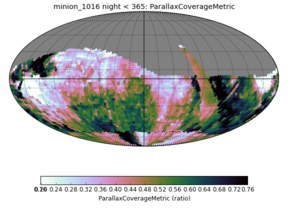
\includegraphics[width=2.0in]{./figs/milkyway/astromPanels/MW_Astrom_paCovge_Baseline_01y_map.png}
  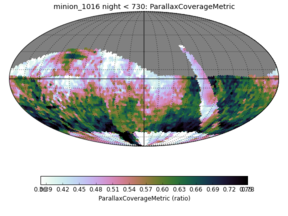
\includegraphics[width=2.0in]{./figs/milkyway/astromPanels/MW_Astrom_paCovge_Baseline_02y_map.png}
  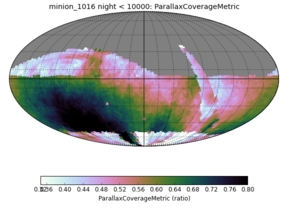
\includegraphics[width=2.0in]{./figs/milkyway/astromPanels/MW_Astrom_paCovge_Baseline_10y_map.png}
  \end{center}
  \begin{center}
  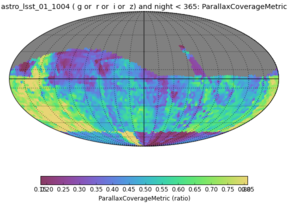
\includegraphics[width=2.0in]{./figs/milkyway/astromPanels/MW_Astrom_paCovge_wfdPlane_01y_map.png}
  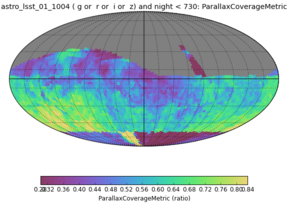
\includegraphics[width=2.0in]{./figs/milkyway/astromPanels/MW_Astrom_paCovge_wfdPlane_02y_map.png}
  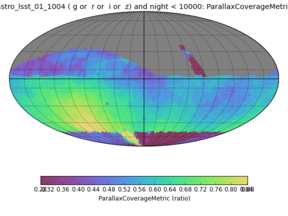
\includegraphics[width=2.0in]{./figs/milkyway/astromPanels/MW_Astrom_paCovge_wfdPlane_10y_map.png}
  \end{center}

  \begin{center}
  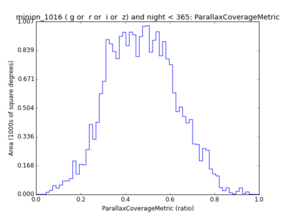
\includegraphics[width=2.0in]{./figs/milkyway/astromPanels/MW_Astrom_paCovge_Baseline_01y_hst.png}
  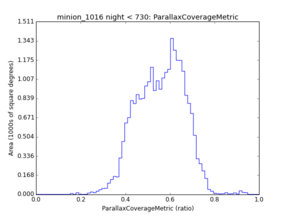
\includegraphics[width=2.0in]{./figs/milkyway/astromPanels/MW_Astrom_paCovge_Baseline_02y_hst.png}
  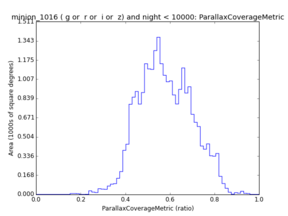
\includegraphics[width=2.0in]{./figs/milkyway/astromPanels/MW_Astrom_paCovge_Baseline_10y_hst.png}
  \end{center}
  \begin{center}
  \includegraphics[width=2.0in]{./figs/milkyway/astromPanels/MW_Astrom_paCovge_wfdPlane_01y_hst.png}
  \includegraphics[width=2.0in]{./figs/milkyway/astromPanels/MW_Astrom_paCovge_wfdPlane_02y_hst.png}
  \includegraphics[width=2.0in]{./figs/milkyway/astromPanels/MW_Astrom_paCovge_wfdPlane_10y_hst.png}
  \end{center}
  \caption{Parallax coverage achieved at different epochs within the survey. {\it Top and Third row:} OpSim run \opsimdbref{db:baseCadence}. {\it Second and bottom row:} OpSim run \opsimdbref{db:NormalGalacticPlane} (wide-fast-deep extended to much of the inner Plane). Reading left-right, columns represent: {\it Left column:} all observations within the first 365 days of operation; {\it Middle column:} first two years; {\it right column:} the full 10-year survey. Spatial maps are clipped at 95\%, with histogram horizontal limits (0.0 - 1.0).}
  \label{fig_astrom_ByTime_PACoverage}
\end{figure}

\begin{figure}[ht]
  \begin{center}
  \includegraphics[width=2.0in]{./figs/milkyway/astromPanels/MW_Astrom_paDcrDegen_Baseline_01y_map.png}
  \includegraphics[width=2.0in]{./figs/milkyway/astromPanels/MW_Astrom_paDcrDegen_Baseline_02y_map.png}
  \includegraphics[width=2.0in]{./figs/milkyway/astromPanels/MW_Astrom_paDcrDegen_Baseline_10y_map.png}
  \end{center}
  \begin{center}
  \includegraphics[width=2.0in]{./figs/milkyway/astromPanels/MW_Astrom_paDcrDegen_wfdPlane_01y_map.png}
  \includegraphics[width=2.0in]{./figs/milkyway/astromPanels/MW_Astrom_paDcrDegen_wfdPlane_02y_map.png}
  \includegraphics[width=2.0in]{./figs/milkyway/astromPanels/MW_Astrom_paDcrDegen_wfdPlane_10y_map.png}
  \end{center}

  \begin{center}
  \includegraphics[width=2.0in]{./figs/milkyway/astromPanels/MW_Astrom_paDcrDegen_Baseline_01y_hst.png}
  \includegraphics[width=2.0in]{./figs/milkyway/astromPanels/MW_Astrom_paDcrDegen_Baseline_02y_hst.png}
  \includegraphics[width=2.0in]{./figs/milkyway/astromPanels/MW_Astrom_paDcrDegen_Baseline_10y_hst.png}
  \end{center}
  \begin{center}
  \includegraphics[width=2.0in]{./figs/milkyway/astromPanels/MW_Astrom_paDcrDegen_wfdPlane_01y_hst.png}
  \includegraphics[width=2.0in]{./figs/milkyway/astromPanels/MW_Astrom_paDcrDegen_wfdPlane_02y_hst.png}
  \includegraphics[width=2.0in]{./figs/milkyway/astromPanels/MW_Astrom_paDcrDegen_wfdPlane_10y_hst.png}
  \end{center}
  \caption{Correlation coefficient $\rho$~between parallax and Differential Chromatic Refraction (DCR) up to different epochs within the survey. {\it Top and Third row:} OpSim run \opsimdbref{db:baseCadence}. {\it Second and bottom row:} OpSim run \opsimdbref{db:NormalGalacticPlane} (wide-fast-deep extended to much of the inner Plane). Reading left-right, columns represent: {\it Left column:} all observations within the first 365 days of operation; {\it Middle column:} first two years; {\it right column:} the full 10-year survey. Spatial maps are clipped at 95\%, with histogram horizontal scale set to the range $-1.0 \le \rho \le +1.0$.}
  \label{fig_astrom_ByTime_PADegen}
\end{figure}



\begin{figure}[ht]
  \begin{center}
  \includegraphics[width=2.0in]{./figs/milkyway/astromPanels/MW_Astrom_pmError_Baseline_01y_map.png}
  \includegraphics[width=2.0in]{./figs/milkyway/astromPanels/MW_Astrom_pmError_Baseline_02y_map.png}
  \includegraphics[width=2.0in]{./figs/milkyway/astromPanels/MW_Astrom_pmError_Baseline_10y_map.png}
  \end{center}
  \begin{center}
  \includegraphics[width=2.0in]{./figs/milkyway/astromPanels/MW_Astrom_pmError_wfdPlane_01y_map.png}
  \includegraphics[width=2.0in]{./figs/milkyway/astromPanels/MW_Astrom_pmError_wfdPlane_02y_map.png}
  \includegraphics[width=2.0in]{./figs/milkyway/astromPanels/MW_Astrom_pmError_wfdPlane_10y_map.png}
  \end{center}

  \begin{center}
  \includegraphics[width=2.0in]{./figs/milkyway/astromPanels/MW_Astrom_pmError_Baseline_01y_hst.png}
  \includegraphics[width=2.0in]{./figs/milkyway/astromPanels/MW_Astrom_pmError_Baseline_02y_hst.png}
  \includegraphics[width=2.0in]{./figs/milkyway/astromPanels/MW_Astrom_pmError_Baseline_10y_hst.png}
  \end{center}
  \begin{center}
  \includegraphics[width=2.0in]{./figs/milkyway/astromPanels/MW_Astrom_pmError_wfdPlane_01y_hst.png}
  \includegraphics[width=2.0in]{./figs/milkyway/astromPanels/MW_Astrom_pmError_wfdPlane_02y_hst.png}
  \includegraphics[width=2.0in]{./figs/milkyway/astromPanels/MW_Astrom_pmError_wfdPlane_10y_hst.png}
  \end{center}
  \caption{Proper motion error for a star at $r=21.0$, for different epochs within the survey. Crowding errors are ignored. {\it Top and Third row:} OpSim run \opsimdbref{db:baseCadence}.  {\it Second and bottom row:} OpSim run \opsimdbref{db:NormalGalacticPlane} (wide-fast-deep extended to much of the inner Plane). Reading left-right, columns represent: {\it Left column:} all observations within the first 365 days of operation; {\it Middle column:} first two years; {\it right column:} the full 10-year survey. Spatial maps are clipped at 95\% and a log-scale is used for the maps and histograms. Reading left-right, the horizontal upper limits on the histograms are (25, 10, 3.0) mas yr$^{-1}$, respectively. Note that the histograms do not include the full range of values reported in the maps.}
  \label{fig_astrom_ByTime_pmError}
\end{figure}


\begin{figure}[ht]
  \begin{center}
  \includegraphics[width=2.0in]{./figs/milkyway/astromPanels/MW_Astrom_paError_Baseline_01y_map.png}
  \includegraphics[width=2.0in]{./figs/milkyway/astromPanels/MW_Astrom_paError_Baseline_02y_map.png}
  \includegraphics[width=2.0in]{./figs/milkyway/astromPanels/MW_Astrom_paError_Baseline_10y_map.png}
  \end{center}
  \begin{center}
  \includegraphics[width=2.0in]{./figs/milkyway/astromPanels/MW_Astrom_paError_wfdPlane_01y_map.png}
  \includegraphics[width=2.0in]{./figs/milkyway/astromPanels/MW_Astrom_paError_wfdPlane_02y_map.png}
  \includegraphics[width=2.0in]{./figs/milkyway/astromPanels/MW_Astrom_paError_wfdPlane_10y_map.png}
  \end{center}

  \begin{center}
  \includegraphics[width=2.0in]{./figs/milkyway/astromPanels/MW_Astrom_paError_Baseline_01y_hst.png}
  \includegraphics[width=2.0in]{./figs/milkyway/astromPanels/MW_Astrom_paError_Baseline_02y_hst.png}
  \includegraphics[width=2.0in]{./figs/milkyway/astromPanels/MW_Astrom_paError_Baseline_10y_hst.png}
  \end{center}
  \begin{center}
  \includegraphics[width=2.0in]{./figs/milkyway/astromPanels/MW_Astrom_paError_wfdPlane_01y_hst.png}
  \includegraphics[width=2.0in]{./figs/milkyway/astromPanels/MW_Astrom_paError_wfdPlane_02y_hst.png}
  \includegraphics[width=2.0in]{./figs/milkyway/astromPanels/MW_Astrom_paError_wfdPlane_10y_hst.png}
  \end{center}
  \caption{Parallax error for a star at $r=21.0$, for different epochs within the survey. Crowding errors are ignored. {\it Top and Third row:} OpSim run \opsimdbref{db:baseCadence}. {\it Second and bottom row:} OpSim run \opsimdbref{db:NormalGalacticPlane} (wide-fast-deep extended to much of the inner Plane). Reading left-right, columns represent: {\it Left column:} all observations within the first 365 days of operation; {\it Middle column:} first two years; {\it right column:} the full 10-year survey. Spatial maps are clipped at 95\%.  Reading left-right, the horizontal upper limits on the histograms are (10, 10, 2.0) mas, respectively.}
  \label{fig_astrom_ByTime_paError}
\end{figure}

%%% Now for the metrics by filter.
\begin{figure}[ht]
  \begin{center}
  \includegraphics[width=2.0in]{./figs/milkyway/astromPanels/MW_Astrom_paCovge_Baseline_u_map.png}
  \includegraphics[width=2.0in]{./figs/milkyway/astromPanels/MW_Astrom_paCovge_Baseline_y_map.png}
  \includegraphics[width=2.0in]{./figs/milkyway/astromPanels/MW_Astrom_paCovge_Baseline_10y_map.png}
  \end{center}
  \begin{center}
  \includegraphics[width=2.0in]{./figs/milkyway/astromPanels/MW_Astrom_paCovge_wfdPlane_u_map.png}
  \includegraphics[width=2.0in]{./figs/milkyway/astromPanels/MW_Astrom_paCovge_wfdPlane_y_map.png}
  \includegraphics[width=2.0in]{./figs/milkyway/astromPanels/MW_Astrom_paCovge_wfdPlane_10y_map.png}
  \end{center}

  \begin{center}
  \includegraphics[width=2.0in]{./figs/milkyway/astromPanels/MW_Astrom_paCovge_Baseline_u_hst.png}
  \includegraphics[width=2.0in]{./figs/milkyway/astromPanels/MW_Astrom_paCovge_Baseline_y_hst.png}
  \includegraphics[width=2.0in]{./figs/milkyway/astromPanels/MW_Astrom_paCovge_Baseline_10y_hst.png}
  \end{center}
  \begin{center}
  \includegraphics[width=2.0in]{./figs/milkyway/astromPanels/MW_Astrom_paCovge_wfdPlane_u_hst.png}
  \includegraphics[width=2.0in]{./figs/milkyway/astromPanels/MW_Astrom_paCovge_wfdPlane_y_hst.png}
  \includegraphics[width=2.0in]{./figs/milkyway/astromPanels/MW_Astrom_paCovge_wfdPlane_10y_hst.png}
  \end{center}
  \caption{Parallax coverage achieved for three extremes of object color, over the full 10-year survey. {\it Top and Third row:} OpSim run \opsimdbref{db:baseCadence}. {\it Second and bottom row:} OpSim run \opsimdbref{db:NormalGalacticPlane} (wide-fast-deep extended to much of the inner Plane). Reading left-right, columns represent: {\it Left column:} Objects detected only in the bluest filter; {\it Middle column:} objects detected only in the reddest filter; {\it Right column:} objects detected in all filters. Spatial maps are clipped at 95\%, with histogram horizontal limits (0.0 - 1.0).}
  \label{fig_astrom_ByFilter_PACoverage}
\end{figure}

\begin{figure}[ht]
  \begin{center}
  \includegraphics[width=2.0in]{./figs/milkyway/astromPanels/MW_Astrom_paDcrDegen_Baseline_u_map.png}
  \includegraphics[width=2.0in]{./figs/milkyway/astromPanels/MW_Astrom_paDcrDegen_Baseline_y_map.png}
  \includegraphics[width=2.0in]{./figs/milkyway/astromPanels/MW_Astrom_paDcrDegen_Baseline_10y_map.png}
  \end{center}
  \begin{center}
  \includegraphics[width=2.0in]{./figs/milkyway/astromPanels/MW_Astrom_paDcrDegen_wfdPlane_u_map.png}
  \includegraphics[width=2.0in]{./figs/milkyway/astromPanels/MW_Astrom_paDcrDegen_wfdPlane_y_map.png}
  \includegraphics[width=2.0in]{./figs/milkyway/astromPanels/MW_Astrom_paDcrDegen_wfdPlane_10y_map.png}
  \end{center}

  \begin{center}
  \includegraphics[width=2.0in]{./figs/milkyway/astromPanels/MW_Astrom_paDcrDegen_Baseline_u_hst.png}
  \includegraphics[width=2.0in]{./figs/milkyway/astromPanels/MW_Astrom_paDcrDegen_Baseline_y_hst.png}
  \includegraphics[width=2.0in]{./figs/milkyway/astromPanels/MW_Astrom_paDcrDegen_Baseline_10y_hst.png}
  \end{center}
  \begin{center}
  \includegraphics[width=2.0in]{./figs/milkyway/astromPanels/MW_Astrom_paDcrDegen_wfdPlane_u_hst.png}
  \includegraphics[width=2.0in]{./figs/milkyway/astromPanels/MW_Astrom_paDcrDegen_wfdPlane_y_hst.png}
  \includegraphics[width=2.0in]{./figs/milkyway/astromPanels/MW_Astrom_paDcrDegen_wfdPlane_10y_hst.png}
  \end{center}
  \caption{Correlation coefficient $\rho$~between parallax and Differential Chromatic Refraction (DCR), selecting filters for three extremes of object color, over the full 10-year survey. {\it Top and Third row:} OpSim run \opsimdbref{db:baseCadence}. {\it Second and bottom row:} OpSim run \opsimdbref{db:NormalGalacticPlane} (wide-fast-deep extended to much of the inner Plane). Reading left-right, columns represent: {\it Left column:} Objects detected only in the bluest filter; {\it Middle column:} objects detected only in the reddest filter; {\it Right column:} objects detected in all filters. Spatial maps are clipped at 95\%, with histogram horizontal scale set to the range $-1.0 \le \rho \le +1.0$.}
  \label{fig_astrom_ByFilter_PADegen}
\end{figure}

\begin{figure}[ht]
  \begin{center}
  \includegraphics[width=2.0in]{./figs/milkyway/astromPanels/MW_Astrom_pmError_Baseline_u_map.png}
  \includegraphics[width=2.0in]{./figs/milkyway/astromPanels/MW_Astrom_pmError_Baseline_y_map.png}
  \includegraphics[width=2.0in]{./figs/milkyway/astromPanels/MW_Astrom_pmError_Baseline_10y_map.png}
  \end{center}
  \begin{center}
  \includegraphics[width=2.0in]{./figs/milkyway/astromPanels/MW_Astrom_pmError_wfdPlane_u_map.png}
  \includegraphics[width=2.0in]{./figs/milkyway/astromPanels/MW_Astrom_pmError_wfdPlane_y_map.png}
  \includegraphics[width=2.0in]{./figs/milkyway/astromPanels/MW_Astrom_pmError_wfdPlane_10y_map.png}
  \end{center}

  \begin{center}
  \includegraphics[width=2.0in]{./figs/milkyway/astromPanels/MW_Astrom_pmError_Baseline_u_hst.png}
  \includegraphics[width=2.0in]{./figs/milkyway/astromPanels/MW_Astrom_pmError_Baseline_y_hst.png}
  \includegraphics[width=2.0in]{./figs/milkyway/astromPanels/MW_Astrom_pmError_Baseline_10y_hst.png}
  \end{center}
  \begin{center}
  \includegraphics[width=2.0in]{./figs/milkyway/astromPanels/MW_Astrom_pmError_wfdPlane_u_hst.png}
  \includegraphics[width=2.0in]{./figs/milkyway/astromPanels/MW_Astrom_pmError_wfdPlane_y_hst.png}
  \includegraphics[width=2.0in]{./figs/milkyway/astromPanels/MW_Astrom_pmError_wfdPlane_10y_hst.png}
  \end{center}
  \caption{Proper motion error for a star at apparent magnitude $m=21.0$, for three extremes of object color and assessed over the full survey. Crowding errors are ignored. {\it Top and Third row:} OpSim run \opsimdbref{db:baseCadence}. {\it Second and bottom row:} OpSim run \opsimdbref{db:NormalGalacticPlane} (wide-fast-deep extended to much of the inner Plane). Reading left-right, columns represent: {\it Left column:} Objects detected only in the bluest filter; the fiducial object has apparent magnitude $u=21.0$; {\it Middle column:} objects detected only in the reddest filter (so $y = 21.0$); {\it Right column:} objects detected in all filters (using $r=21.0$~and a ``flat'' spectrum within sims\_maf). Spatial maps are clipped at 95\% and a log-scale is used for both the spatial maps and histograms. Reading left-right, the horizontal upper limits on the histograms are (4.0, 4.0, 3.0) mas yr$^{-1}$, respectively. Note that the histograms do not include the full range of values reported in the maps.}
  \label{fig_astrom_ByFilter_pmError}
\end{figure}

\begin{figure}[ht]
  \begin{center}
  \includegraphics[width=2.0in]{./figs/milkyway/astromPanels/MW_Astrom_paError_Baseline_u_map.png}
  \includegraphics[width=2.0in]{./figs/milkyway/astromPanels/MW_Astrom_paError_Baseline_y_map.png}
  \includegraphics[width=2.0in]{./figs/milkyway/astromPanels/MW_Astrom_paError_Baseline_10y_map.png}
  \end{center}
  \begin{center}
  \includegraphics[width=2.0in]{./figs/milkyway/astromPanels/MW_Astrom_paError_wfdPlane_u_map.png}
  \includegraphics[width=2.0in]{./figs/milkyway/astromPanels/MW_Astrom_paError_wfdPlane_y_map.png}
  \includegraphics[width=2.0in]{./figs/milkyway/astromPanels/MW_Astrom_paError_wfdPlane_10y_map.png}
  \end{center}

  \begin{center}
  \includegraphics[width=2.0in]{./figs/milkyway/astromPanels/MW_Astrom_paError_Baseline_u_hst.png}
  \includegraphics[width=2.0in]{./figs/milkyway/astromPanels/MW_Astrom_paError_Baseline_y_hst.png}
  \includegraphics[width=2.0in]{./figs/milkyway/astromPanels/MW_Astrom_paError_Baseline_10y_hst.png}
  \end{center}
  \begin{center}
  \includegraphics[width=2.0in]{./figs/milkyway/astromPanels/MW_Astrom_paError_wfdPlane_u_hst.png}
  \includegraphics[width=2.0in]{./figs/milkyway/astromPanels/MW_Astrom_paError_wfdPlane_y_hst.png}
  \includegraphics[width=2.0in]{./figs/milkyway/astromPanels/MW_Astrom_paError_wfdPlane_10y_hst.png}
  \end{center}
  \caption{Parallax error for a star at apparent magnitude $m=21.0$, for three extremes of object color and assessed over the full survey. Crowding errors are ignored. {\it Top and Third row:} OpSim run \opsimdbref{db:baseCadence}. {\it Second and bottom row:} OpSim run \opsimdbref{db:NormalGalacticPlane} (wide-fast-deep extended to much of the inner Plane). Reading left-right, columns represent: {\it Left column:} Objects detected only in the bluest filter; the fiducial object has apparent magnitude $u=21.0$; {\it Middle column:} objects detected only in the reddest filter (so $y = 21.0$); {\it Right column:} objects detected in all filters (using $r=21.0$~and a ``flat'' spectrum within sims\_maf). Spatial maps are clipped at 95\%. Reading left-right, the horizontal upper limits on the histograms are (10, 10, 2.0) mas, respectively. Note that the histograms do not include the full range of values reported in the maps.}
  \label{fig_astrom_ByFilter_paError}
\end{figure}

\subsubsection{Figures of Merit depending on the Metrics}

Building on the first-order metrics above, this subsection communicates scientific figures of merit for the cases identified in \autoref{sec:\secname:MW_Astrometry_measurements} above.

Table \ref{tab_SummaryMWAstrometry} summarizes the Figures of Merit
(FoMs) for Astrometry science cases. At the time of writing, FoMs have
been implemented to summarize the random uncertainty in proper motion
and parallax, for two regions experiencing extreme values of these
quantities: the inner Plane (conservatively defined in this section as
$|b| \lesssim 7^o$~and $|l| \lesssim 80^o$), and the main survey
(excluding the inner plane and the Southern Polar region, taken
here as $\delta_{2000.0} < -60.0^o$). Figure
\ref{fig_astrom_RegionSelKey} illustrates these selection-regions on
the sky. These form FoM 1.1-1.4, and have to-date been run for the
OpSim runs \opsimdbref{db:baseCadence} (Baseline cadence),
\opsimdbref{db:opstwoPS} (similar to PanSTARRS-1), and the
recently-completed \opsimdbref{db:NormalGalacticPlane} (which applies
Wide-Fast-Deep cadence to much of the inner Galactic Plane). From the point of
view of parallax and proper motion, the latter two strategies do not
negatively impact the non-plane regions, but they {\it substantially}
improve the sampling for proper motions and parallax (again,
neglecting the effects of spatial crowding).

FoM 1.5 in Table \ref{tab_SummaryMWAstrometry} reports the total number of fields with Parallax/Hour-angle correlation $|\rho| < 0.7$.

At the time of writing, FoMs 2-5 in Table
\ref{tab_SummaryMWAstrometry} are still at the specification stage,
and are described in Section
\ref{sec:\secname:MW_Astrometry_furtherwork}.

%%%% Figures used as ``key'' for the astrometry FoMs:

\begin{figure}[h]
  \begin{center}
    \includegraphics[width=2.0in]{./figs/milkyway/astromPanels/MW_Astrom_FoM_properMotion_minion_1016_all_skymap.png}
  \includegraphics[width=2.0in]{./figs/milkyway/astromPanels/MW_Astrom_FoM_properMotion_minion_1016_plane_skymap.png}
  \includegraphics[width=2.0in]{./figs/milkyway/astromPanels/MW_Astrom_FoM_properMotion_minion_1016_nonPlane_skymap.png}
    \end{center}
  \caption{Selection regions for the Astrometry Figures of Merit (FoMs) 1.1-1.4. Figures of Merit 1.1 and 1.3 refer to the ``main survey'' region shown in the middle panel (which for the FoM also avoids the region of the South Galactic Pole). The right panel shows the inner Plane region to which FoMs 1.2 \& 1.4 refer. The left-hand panel shows the entire survey region for reference. This example shows run \opsimdbref{db:baseCadence}. See Table \ref{tab_SummaryMWAstrometry} and Section \ref{sec:\secname:MW_Astrometry_metrics}.}
  \label{fig_astrom_RegionSelKey}
\end{figure}

\subsection{Topics that will need to be addressed}
\label{sec:\secname:MW_Astrometry_furtherwork}

Here we present suggestions for further work, first on figures of
merit for the science cases, and then on additional Metrics for LSST's
astrometric performance.

\subsubsection{Further work on science Figures of Merit}
%\medskip

At the time of writing, the Figures of Merit for both the highlighted
Science cases need to be implemented and applied to OpSim output,
preferably in a format that can be summarized in a single Table in
this section. These figures of merit are discussed above in Section
\ref{sec:\secname:MW_Astrometry_metrics} (particularly for the Halo
Streams science project). Figures of merit for the two science cases
might be:
\begin{itemize}
  \item[1.] Number of streams that LSST can discover via their proper motions;
\item[2.] Uncertainty and bias in the thin and thick disk differential age measurement when using white dwarfs from each population as tracers.
\end{itemize}

Given the diversity of science cases that use local Solar Neighborhood
populations as tracers, it may be advantageous to subdivide the Solar
Neighborhood projects into further figures of merit. Two further example
figures of merit might then be:
\begin{itemize}
  \item[3.] Uncertainty and bias in the Brown Dwarf mass function using Solar Neighborhood tracers;
   \item[4.] Uncertainty and bias in the thickness in the main sequence of M-dwarfs within 25pc from the Sun, once variability has been characterized and removed.
\end{itemize}

%%%% SUMMARY TABLE FOR THIS SECTION

\begin{table}
  \begin{tabular}{l|p{4.8cm}|p{1.1cm}|p{1.1cm}|p{1.1cm}|c|p{3.5cm}}
    FoM & Brief description & {\rotatebox{90}{\opsimdbref{db:baseCadence} }} & {\rotatebox{90}{\opsimdbref{db:opstwoPS} }} & {\rotatebox{90}{\opsimdbref{db:NormalGalacticPlane}   }} &  {\rotatebox{90}{future run 2}} & Notes \\
    \hline
    1.1 & \footnotesize{Median parallax error at $r=21$ (main survey)}      & 0.69  & 0.72 & 0.69 & - &
%\footnotesize{Summarize the presentation in Figures \ref{fig_astrom_ByTime_PACoverage}-\ref{fig_astrom_ByFilter_paError} }
\footnotesize{See region definitions in Figure \ref{fig_astrom_RegionSelKey}.}
\\
    1.2. & \footnotesize{Median parallax error at $r=21$ (plane)}   & 2.68 & {\bf 0.91} & {\bf 0.89} & - &
\footnotesize{Smaller values are better.}\\
    1.3. & \footnotesize{Median proper motion error at $r=21$ (main survey)}  & 0.19 & 0.19 & 0.19 & - &
%\footnotesize{Take median of Figure \ref{fig_astrom_ByTime_pmError} over the ``plane'' region.}
\\
    1.4. & \footnotesize{Median proper motion error at $r=21$ (plane)} & 16.7
%$^\dagger$
& {\bf 0.26} & {\bf 0.25} & - &
%\footnotesize{$^\dagger$no, this is not a typo.}
\\
1.5. & \footnotesize{Fields with Parallax-DCR correlation coefficient $\rho \ge 0.7$~/ total fields} & \footnotesize{ \bf{3486} / \bf {31116} } & \footnotesize{3586 / 30107} & \footnotesize{3690 / 31116} & - & \footnotesize{Smaller is better. Value reported after full 10 years of survey for $griz$~detections.}  \\
    \hline
    2.1. & \footnotesize{Number of streams LSST can discover via proper motions} & - & - & - & - &  - \\
    3.1. & \footnotesize{Uncertainty and bias in thin- and thick-disk differential age measurement via white dwarfs} & - & - & - & - &  - \\
    4.1. & \footnotesize{Uncertainty and bias in brown dwarf mass function from the Solar Neighborhood}  & - & - & - & - & \footnotesize{Using astrometry metrics for objects detected only in the reddest filter(s)} \\
    4.2. & \footnotesize{Uncertainty and bias in white dwarf mass function from the Solar Neighborhood}  & - & - & - & - & \footnotesize{Using astrometry metrics for objects detected only in the bluest filter(s)} \\
    5.1. & \footnotesize{Uncertainty and bias in Solar Neighborhood M-dwarf thickness on the MS}  & - & - & - & - &  - \\
\end{tabular}
\caption{Summary of Figures of Merit for the Milky Way Astrometry science cases. The best value of each FoM is indicated in bold. Runs \opsimdbref{db:baseCadence} and \opsimdbref{db:opstwoPS} refer to the Baseline and PanSTARRS-like strategies, respectively. Column \opsimdbref{db:NormalGalacticPlane} refers to a recently-completed OpSim run that includes the Plane in Wide-Fast-Deep observations. See \autoref{sec:MW_Astrometry}.}
\label{tab_SummaryMWAstrometry}
\end{table}


%%%% SUMMARY TABLE FINISHES HERE


\subsubsection{Further work on Astrometry Metrics}

The MAF metrics presented in Sections \ref{sec:\secname:MW_Astrometry_OpSim} and \ref{sec:\secname:MW_Astrometry_metrics} are only part of the
study of LSST's predicted astrometric performance.  Detailed simulations
and studies need to be done in many other areas as part of the
prediction and verification of LSST's astrometric performance.  Among
the most important are the following.
\begin{itemize}
\item How well do galaxies perform as astrometric reference objects? Are certain shapes or colors better than others? What is the
surface density of ``good" astrometric reference galaxies as a function of filter?
\item How well can we identify optically point-like QSOs that will be useful in matching the optical reference frame to the ICRS?
%\item Given the LSST exposure time, site, and physical characteristics, how can we mitigate the limitations on astrometric accuracy imposed by the seeing and local atmospheric turbulence?
\item How does the astrometric performance depend on stellar density? If there are fields in which photometry is only possible via difference imaging, what are the limitations
on astrometry in these fields?
%\item What tools do we need to compare the general and specific agreement between the {\it Gaia} results and the LSST results?
\item Does the ``brighter-wider" effect in the deep-depletion CCDs introduce a magnitude term into the centroid positions?
\end{itemize}

% ====================================================================

\subsection{Conclusions}

Here we answer the ten questions posed in
\autoref{sec:intro:evaluation:caseConclusions}:

\begin{description}

\item[Q1:] {\it Does the science case place any constraints on the
tradeoff between the sky coverage and coadded depth? For example, should
the sky coverage be maximized (to $\sim$30,000 deg$^2$, as e.g., in
Pan-STARRS) or the number of detected galaxies (the current baseline but
with 18,000 deg$^2$)?}

\new{ \item[A1:] We do expect tradeoffs between depth and sky
  coverage, but we do not yet have the FoM evaluations to set
  quantitative constraints. For example, we expect some combination of
  depth and survey volume would optimize the completeness to objects
  among the populations in the Solar Neighborhood. More generally,
  perhaps, in fields away from the galactic mid-plane, the
  lengthscales over which the proper motion zeropoints can be
  accurately constrained will depend on the spatial density of
  well-measured background galaxies (finer lengthscale corresponding
  to greater co-added depth). The depth must therefore be sufficient
  to sample enough of these galaxies to constrain variations of
  astrometric zeropoint on lengthscales at least as fine as those
  imposed by the LSST system itself (or the atmosphere, whichever is
  finer). We anticipate that this tradeoff can be informed by
  simulation under a set of assumptions for these variations.}

\item[Q2:] {\it Does the science case place any constraints on the
tradeoff between uniformity of sampling and frequency of  sampling? For
example, a rolling cadence can provide enhanced sample rates over a part
of the survey or the entire survey for a designated time at the cost of
reduced sample rate the rest of the time (while maintaining the nominal
total visit counts).}

\new{ \item[A2:] Yes, although for astrometry the language of these
  constraints is slightly different. The parallactic ellipse must be
  sufficiently covered, the correlation between hour angle and
  parallax factor must be minimized, and the visits must be
  sufficiently distributed (both within a year and over the ten-year
  time baseline) to produce the best precision in both proper motion and parallax. See Section \ref{sec:MW_Astrometry:MW_Astrometry_metrics}}.

\item[Q3:] {\it Does the science case place any constraints on the
tradeoff between the single-visit depth and the number of visits
(especially in the $u$-band where longer exposures would minimize the
impact of the readout noise)?}

\new{ \item[A3:] More visits at the standard exposure time are
  generally preferred to a few visits with longer exposures, in order
  to achieve as broad a temporal coverage as possible (see Section
  \ref{sec:MW_Astrometry:MW_Astrometry_metrics}). The $u$-band itself
  is likely to be of limited use for astrometry (except possibly for
  extremely blue objects with little signal in any of the other
  filters) due to differential chromatic refraction (DCR), however of
  course $u$-band will still be useful for photometric constraints.}

\item[Q4:] {\it Does the science case place any constraints on the
Galactic plane coverage (spatial coverage, temporal sampling, visits per
band)?}

\new{ \item[A4:] Not for the example of detecting Galactic Halo
  streams via proper motions (Section
  \ref{sec:MW_Astrometry:MW_Astrometry_measurements}). For the Solar
  Neighborhood populations, avoiding the inner Galactic mid-plane
  would obviously reduce the completeness of the census of nearby
  objects with parallax determinations due to the reduction in total
  area surveyed. However, this reduction may be incremental rather
  than serious. The impact of an inner-plane zone of avoidance on the
  recovery of the parameters describing these constituent populations
  has not yet been evaluated. Of course, this all changes for
  astrometry of objects of interest that lie in the inner plane (see
  also Section \ref{sec:MW_Disk}), where (for example) the reduced
  proper motion will be a useful diagnostic. At present, however, the
  performance of the LSST software stack towards crowded fields is
  as-yet unknown. As this performance becomes better understood, it
  will be possible to quantitatively compare strategies for astrometry
  towards the inner plane.}

\item[Q5:] {\it Does the science case place any constraints on the
fraction of observing time allocated to each band?}

\new{ \item[A5:] Yes, but indirectly through the requirement to
  measure all the populations of interest in the Solar
  Neighborhood. Making the assumption that this science case requires
  parallax measurements for extremely blue objects as well as
  extremely red objects, which might each be measurable only in a
  single very red or blue filter, would suggest at a minimum that the
  coverage considerations of Section
  \ref{sec:MW_Astrometry:MW_Astrometry_metrics} be applied to
  observations in $u$~and $Y$ filters separately, as well as at least
  one mid-range filter. However the quantitative impact on population
  recovery from various filter-distributions has yet to be assessed at
  this date. Further work is needed to determine if the increased
  sensitivity of $u$-band astrometry to DCR relative to $g$-band would
  prevent its use for astrometry.}

\item[Q6:] {\it Does the science case place any constraints on the
cadence for deep drilling fields?}

\new{ \item[A6:] If precision astrometry is desired for the deep drilling fields, then the considerations of Section \ref{sec:MW_Astrometry:MW_Astrometry_metrics} apply to those fields as well.}

\item[Q7:] {\it Assuming two visits per night, would the science case
benefit if they are obtained in the same band or not?}

\new{ \item[A7:] While detailed investigation is still pending, we
  expect that using different filters within the same night would be
  preferred to allow better constraint of DCR effects. Doing different
  filters on the same night might reduce the number of free parameters
  (like seeing and parallax factor) and give more pairs for direct
  filter-A vs. filter-B astrometry.}

\item[Q8:] {\it Will the case science benefit from a special cadence
prescription during commissioning or early in the survey, such as:
acquiring a full 10-year count of visits for a small area (either in all
the bands or in a  selected set); a greatly enhanced cadence for a small
area?}

\new{ \item[A8:] It is vital for astrometry that at least a few fields
  be observed with both sufficient parallax factor coverage and
  sufficient number of visits, early in the survey, to demonstrate
  parallax precision specified in the Science Requirements
  Document. In these fields, sufficient exposures must be reserved for
  the entire 10-year survey baseline so that proper motion precision
  is not too badly compromised in these fields. This combination of
  factors may require dedicated commissioning observations of these
  fields in addition to the 10-year survey operations. In addition,
  however, at least a few fields must be observed at a variety of
  values of single-visit achieved depth, and FWHM, in order to
  constrain the degree to which FWHM will actually predict the
  achieved astrometric precision (see also the answer to Q10
  below). This second set of requirements may also be best served by
  dedicated commissioning observations.}

\item[Q9:] {\it Does the science case place any constraints on the
sampling of observing conditions (e.g., seeing, dark sky, airmass),
possibly as a function of band, etc.?}

\new{ \item[A9:] The observations need to be planned in such a way
  that the correlation between parallax and hour-angle is minimized,
  to avoid deneracies between the motion due to atmospheric refraction and the motion that is sought due to parallax. See
  Section \ref{sec:MW_Astrometry:MW_Astrometry_metrics}.}

\item[Q10:] {\it Does the case have science drivers that would require
real-time exposure time optimization to obtain nearly constant
single-visit limiting depth?}

\new{ \item[A10:] While optimization on an exposure-to-exposure basis
  is perhaps unlikely, {\it selection} between observations in
  response to conditions (on a timescale of perhaps 10 minutes) will
  be crucial to maximize achieved astrometric precision. The rules by
  which this selection would proceed, still need to be charted. For
  example, while maintaining limiting depth might suggest shorter
  exposure times when the FWHM is narrow, this may not translate to
  improved astrometric error across an LSST chip, because the
  lengthscales of the turbulence driving the FWHM is not the same as
  that of the turbulence driving astrometric error across an LSST chip.}

\end{description}

\navigationbar

% --------------------------------------------------------------------

% ====================================================================
%+
% SECTION:
%    section-name.tex  % eg lenstimedelays.tex
%
% CHAPTER:
%    chapter.tex  % eg cosmology.tex
%
% ELEVATOR PITCH:
%    Explain in a few sentences what the relevant discovery or
%    measurement is going to be discussed, and what will be important
%    about it. This is for the browsing reader to get a quick feel
%    for what this section is about.
%
% COMMENTS:
%
%
% BUGS:
%
%
% AUTHORS:
%    Phil Marshall (@drphilmarshall)  - put your name and GitHub username here!
%-
% ====================================================================

\section{Mapping the Milky Way Bulge}
\def\secname{MW_Bulge}\label{sec:\secname} % For example, replace "keyword" with "lenstimedelays"

\noindent{\it Will Clarkson, ...}  % (Writing team)

% This individual section will need to describe the particular
% discoveries and measurements that are being targeted in this section's
% science case. It will be helpful to think of a ``science case" as a
% ``science project" that the authors {\it actually plan to do}. Then,
% the sections can follow the tried and tested format of an observing
% proposal: a brief description of the investigation, with references,
% followed by a technical feasibility piece. This latter part will need
% to be quantified using the MAF framework, via a set of metrics that
% need to be computed for any given observing strategy to quantify its
% impact on the described science case. Ideally, these metrics would be
% combined in a well-motivated figure of merit. The section can conclude
% with a discussion of any risks that have been identified, and how
% these could be mitigated.

A short preamble goes here. What's the context for this science
project? Where does it fit in the big picture?

% --------------------------------------------------------------------

\subsection{Target measurements and discoveries}
\label{sec:\secname:MW_Bulge_targets}

Describe the discoveries and measurements you want to make.

Now, describe their response to the observing strategy. Qualitatively,
how will the science project be affected by the observing schedule and
conditions? In broad terms, how would we expect the observing strategy
to be optimized for this science?


% --------------------------------------------------------------------

\subsection{Metrics}
\label{sec:\secname:MW_Bulge_metrics}

Quantifying the response via MAF metrics: definition of the metrics,
and any derived overall figure of merit.


% --------------------------------------------------------------------

\subsection{OpSim Analysis}
\label{sec:\secname:MW_Bulge_analysis}

OpSim analysis: how good would the default observing strategy be, at
the time of writing for this science project?


% --------------------------------------------------------------------

\subsection{Discussion}
\label{sec:\secname:MW_Bulge_discussion}

Discussion: what risks have been identified? What suggestions could be
made to improve this science project's figure of merit, and mitigate
the identified risks?


% ====================================================================

\navigationbar

% ====================================================================
%+
% SECTION:
%    section-name.tex  % eg lenstimedelays.tex
%
% CHAPTER:
%    chapter.tex  % eg cosmology.tex
%
% ELEVATOR PITCH:
%    Explain in a few sentences what the relevant discovery or
%    measurement is going to be discussed, and what will be important
%    about it. This is for the browsing reader to get a quick feel
%    for what this section is about.
%
% COMMENTS:
%
%
% BUGS:
%
%
% AUTHORS:
%    Phil Marshall (@drphilmarshall)  - put your name and GitHub username here!
%-
% ====================================================================

\section{Mapping the Local Volume with Resolved Stars}
\def\secname{MW_LocalVolume}\label{sec:\secname} % For example, replace "keyword" with "lenstimedelays"

\noindent{\it ???, ...}  % (Writing team)

% This individual section will need to describe the particular
% discoveries and measurements that are being targeted in this section's
% science case. It will be helpful to think of a ``science case" as a
% ``science project" that the authors {\it actually plan to do}. Then,
% the sections can follow the tried and tested format of an observing
% proposal: a brief description of the investigation, with references,
% followed by a technical feasibility piece. This latter part will need
% to be quantified using the MAF framework, via a set of metrics that
% need to be computed for any given observing strategy to quantify its
% impact on the described science case. Ideally, these metrics would be
% combined in a well-motivated figure of merit. The section can conclude
% with a discussion of any risks that have been identified, and how
% these could be mitigated.

A short preamble goes here. What's the context for this science
project? Where does it fit in the big picture?

% --------------------------------------------------------------------

\subsection{Target measurements and discoveries}
\label{sec:\secname:MW_LocalVolume_targets}

Describe the discoveries and measurements you want to make.

Now, describe their response to the observing strategy. Qualitatively,
how will the science project be affected by the observing schedule and
conditions? In broad terms, how would we expect the observing strategy
to be optimized for this science?


% --------------------------------------------------------------------

\subsection{Metrics}
\label{sec:\secname:MW_LocalVolume_metrics}

Quantifying the response via MAF metrics: definition of the metrics,
and any derived overall figure of merit.


% --------------------------------------------------------------------

\subsection{OpSim Analysis}
\label{sec:\secname:MW_LocalVolume_analysis}

OpSim analysis: how good would the default observing strategy be, at
the time of writing for this science project?


% --------------------------------------------------------------------

\subsection{Discussion}
\label{sec:\secname:MW_LocalVolume_discussion}

Discussion: what risks have been identified? What suggestions could be
made to improve this science project's figure of merit, and mitigate
the identified risks?


% ====================================================================

\navigationbar



% --------------------------------------------------------------------

% --------------------------------------------------------------------

\chapter[Variable Objects]{Variable Objects}
\def\chpname{variables}\label{chp:\chpname}

Chapter editors:
\credit{AshishMahabal},
\credit{lmwalkowicz}.

% \noindent {\it
% Mike Lund, Ashish Mahabal, Stephen Ridgway,
% Lucianne Walkowicz, Rahul Biswas, Michelle Lochner,
% Jeonghee Rho, Eric Bellm...
% }

% --------------------------------------------------------------------


\section{Introduction}

Variable objects are defined as those that exhibit brightness changes, either periodic or non-periodic, which are detected in quiescence and non-destructive to the object itself. Variable objects span a wide range in timescale-of-interest (sometimes even within a single class of objects), and so different science cases benefit from different sampling strategies. These strategies may be significantly disparate from one another, sometimes even mutually exclusive; competing objectives described in this chapter and the next are therefore at the heart of LSST observing strategy and cadence design.

Below we develop a number of key science cases for LSST studies of variable objects, associating them with related metrics that can be used within the Metrics Analysis Framework (MAF) to understand the impact of a given survey strategy realization on the scientific results for that case. The science cases outlined are by no means exhaustive, but rather are motivated by providing key quantitative examples of LSST's performance given any particular deployment of survey strategy. The authors encourage community contribution of similar cases, where the scientific outcome can be quantified using specific metrics.



%When evaluating a particular observation or series of observations in
%light of how they perform for a specific science case, it may be
%helpful to think of metrics as lying along a continuum between
%discovery and characterization. Discovery requires a minimum amount of
%information to recognize an event or object as a candidate of
%interest, which necessarily involves some level of bare-bones
%characterization (upon which said recognition is based); rich
%characterization, on the other hand, implies that an event may not
%only be recognized as a candidate of interest, but basic properties of
%the event or object may be determined from the observation (e.g.
%including but not limited to classification of the event). The
%interpretation of a given metric along this continuum has implications
%for the subsequent action and analysis required, particularly as
%regards possible follow-up observations with other facilities.

%Target types are here grouped in subsections by variability
%characteristics, but as will be seen, this does not mean that all
%targets in a group require a common cadence, since the times scales
%may vary dramatically.  Acquiring suitable data for a wide range of
%time scales presents a fundamental problem for LSST, since the
%available $~$800 visits to a field over the survey cannot be deployed
%so as to usefully sample all time scales at all times.  This fact
%leads to the concept of a non-uniform survey, in which parts of the
%sky are visited more frequently part of the time.  The merits of such
%options must be traded against the benefits of a more uniform survey
%strategy.

\begin{center}
\begin{tabular}{| l | p{8cm} |l | l |}
\hline Periodic Variable Type & Examples of target science & Amplitude & Timescale\\
\hline
RR Lyrae & Galactic structure, distance ladder, RR Lyrae properties&  large &  day \\
Cepheids & Distance ladder, cepheid properties&  large &  day \\
Long Period Variables & Distance ladder, LPV properties & large  &  weeks \\
Short period pulsators & Instability strip, white dwarf interior properties, evolution&  small & min  \\
Periodic binaries & Eclipses, physical properties of stars, distances, ages, evolution, apsidal precession, mass transfer induced period changes, Applegate effect &  small &  hr-day \\
Rotational Modulation & Gyrochronology, stellar activity& small  &  days \\
Young stellar populations & Star and planet formation, accretion physics & small  &  min-days \\
 \hline \end{tabular}
 \end{center}

\subsection{Description of Relevant Metrics}
\label{sec:keyword:variablemetrics}

Despite the range in scientific motivation for the cases presented below, there are some common metrics that are widely applicable (or may be combined in a variety of ways with other metrics to suit a variety of applications).

%\subsection{Metrics}
%\label{sec:keyword:metrics}

\begin{center}
\begin{tabular}{| p{5cm} |p{10cm} |}
\hline Metric & Description\\
\hline
Eclipsing/transiting system discovery & Fraction of discoveries vs fractional duration of eclipse\\
Lightcurve shape recovery & ... \\
%Transiting exoplanets (depth dependent) & Fraction of discoveries vs fractional duration of eclipse\\
Phase gap & Histogram vs period of the median and maximum phase gaps achieved in all fields\\
Period determination (period dependent) & Fraction of targets vs survey duration, for which the period can be determined to 5-sigma confidence\\
Period variability (period dependent) & Fraction of targets vs survey duration, for which a period change of 1\% can be determined with 5-sigma confidence\\
  \hline \end{tabular}
 \end{center}

The ability to identify that an object is periodic, and to correctly determine that object's period, are widely applicable measures of discovery. In the case of regular variables (as outlined below), these two measures together can uniquely identify a population. Other kinds of periodic systems (transiting planets for example) also require a measurement of periodicity, but have a much wider range of relevant periods, and looser requirements on the strictness of that periodicity.

Lund et al. (2015; \url{http://arxiv.org/pdf/1508.03175.pdf}) discuss three metrics that have been incorporated into the MAF. Two of these metrics deal explicitly with time variable behavior: a) observational triplets, and b) detection of periodic variability.

%%%%%%%%%%%%%%%%%%%%%%%%%%%%%%%%%
\begin{figure}[tbh!]
%\vskip -4.1in
%\hskip -0.5in
%\includegraphics[angle=0,width=1.19\hsize:,clip]{figs/enigma1189_earlySNe.pdf}
%\vskip -4.0in
\includegraphics{figs/variables/enigma_1189_PeriodogramPurity_OPSI_SkyMap.pdf}
\caption{The value for the Periodogram Purity Function for candidate Baseline Cadence \opsimdbref{db:enigma}.
The Periodogram Purity Function provides a measure of the power lost due to aliasing.}
\label{fig:enigmaPeriodogramPurity}
\end{figure}
%%%%%%%%%%%%%%%%%%%%%%%%%%%%%%%%%


%%%%%%%%%%%%%%%%%%%%%%%%%%%%%%%%%
\begin{figure}[tbh!]
%\vskip -4.1in
%\hskip -0.5in
%\includegraphics[angle=0,width=1.19\hsize:,clip]{figs/enigma1189_earlySNe.pdf}
%\vskip -4.0in
\includegraphics{figs/variables/enigma_1189_Phase_Gap_MedianGap_OPSI_SkyMap.pdf}
\caption{The median phase gap for candidate Baseline Cadence \opsimdbref{db:enigma}.
The PhaseGapMetric looks at periods between 3 and 35 days by default.}
\label{fig:enigmaMedianGap}
\end{figure}
%%%%%%%%%%%%%%%%%%%%%%%%%%%%%%%%%

%%%%%%%%%%%%%%%%%%%%%%%%%%%%%%%%%
\begin{figure}[tbh!]
%\vskip -4.1in
%\hskip -0.5in
%\includegraphics[angle=0,width=1.19\hsize:,clip]{figs/enigma1189_earlySNe.pdf}
%\vskip -4.0in
\includegraphics{figs/variables/enigma_1189_Phase_Gap_LargestGap_OPSI_SkyMap.pdf}
\caption{The maximum phase gap for candidate Baseline Cadence \opsimdbref{db:enigma}.
The PhaseGapMetric looks at periods between 3 and 35 days by default.}
\label{fig:enigmaMaxGap}
\end{figure}
%%%%%%%%%%%%%%%%%%%%%%%%%%%%%%%%%

\subsubsection{Periodogram purity function (PeriodicMetric)}
This metric calculates the Fourier power spectral window function of each field (Roberts et al. 1987) as a means of quantifying the completeness of phase coverage for a given periodic variable. The periodogram purity is defined as 1 minus the Fourier power spectral window function. in the perfect case, all power in the window function is concentrated in a delta function at zero, and is zero at all other frequencies. As power ``leaks'' away from the correct frequency as a consequence of discrete, non-ideal data sampling, the periodogram becomes more structured. For the purposes of MAF metrics, which are designed to quantify performance as a single number, the periodogram purity is quantified as the minimum value of the periodogram purity function at non-zero frequency shifts; the ideal case would be a periodogram purity metric value of 1.

\subsubsection{Phase Gap Metric (PhaseGapMetric)}

The Phase Gap Metric is designed to examine the largest phase gaps in the observing schedule. For a given point in the sky, a series of periods are randomly selected (by default, 5 periods), with a default minimum of 3 days and maximum of 35 days. The largest phase gap for each period is calculated, and the metric plots the median (\autoref{fig:enigmaMediangap}) and maximum (\autoref{fig:enigmaMediangap}) of this subset of values that contains the maximum phase gap per period. The Phase Gap Metric is part of varMetrics.

\subsubsection{Period Deviation Metric (PeriodDeviationMetric)}

The Period Deviation Metric calculates the error in recovering the correct period of sinusoid using a given observing schedule and a Lomb-Scargle periodogram. For a given point in the sky, a series of periods are randomly selected (by default, 5 periods), and the metric returns the worst period deviation, and the period at which this occurred. The Period Deviation Metric is part of varMetrics.

%\subsection{Proposed Metrics}

%The following is a raw list of metric ideas; these need specificity and further description.

%FWHM of the window function (to quantify sampling)

%Maximum hour angle difference

%Fraction of discoveries vs fractional duration of eclipse

%Fraction of targets vs survey duration, for which the period can be determined to 5-sigma confidence

%Fraction of targets vs survey duration, for which a period change of 1$\%$ can be determined with 5-sigma confidence




% --------------------------------------------------------------------


% ====================================================================
%+
% NAME:
%    section-name.tex
%
% ELEVATOR PITCH:
%    Explain in a few sentences what the relevant discovery or
%    measurement is going to be discussed, and what will be important
%    about it. This is for the browsing reader to get a quick feel
%    for what this section is about.
%
% COMMENTS:
%
%
% BUGS:
%
%
% AUTHORS:
%    Phil Marshall (@drphilmarshall)  - put your name and GitHub username here!
%-
% ====================================================================

\section{Discovery of Periodic Pulsating Variables}
\def\secname{periodicvariables}\label{sec:\secname}

\noindent{\it Lucianne M. Walkowicz, Stephen Ridgway, \&c} % (Writing team)

% This individual section will need to describe the particular
% discoveries and measurements that are being targeted in this section's
% science case. It will be helpful to think of a ``science case" as a
% ``science project" that the authors {\it actually plan to do}. Then,
% the sections can follow the tried and tested format of an observing
% proposal: a brief description of the investigation, with references,
% followed by a technical feasibility piece. This latter part will need
% to be quantified using the MAF framework, via a set of metrics that
% need to be computed for any given observing strategy to quantify its
% impact on the described science case. Ideally, these metrics would be
% combined in a well-motivated figure of merit. The section can conclude
% with a discussion of any risks that have been identified, and how
% these could be mitigated.

Regular variables, such as Cepheids and RR Lyraes, are valuable tracers of Galactic structure and cosmic distance. In this case of these and other strictly (or nearly-strictly) periodic variables, data from different cycles of observation can be phase-folded to create a more fully sampled lightcurve as LSST visits will occur effectively at random phases. In a 10-year survey, most periodic stars of almost any period will benefit from excellent phase coverage in all filters (only a very small period range close to the sidereal day will be poorly observed). Therefore, most implementations of the LSST observing strategy will provide good sampling of periodic variables.

However, different implementations of the survey may result in different resulting sample sizes of these periodic variables, and may also affect the environments in which these stars are discovered. In this section, we create a framework for understanding how current implementations of the observing strategy influence (or even bias) the resultant sample size and environments where these important tracers may be identified. 

\subsection{Tracing Galactic Structure with RR Lyrae}

Oluseyi et al. 2012 [INSERT REF] carried out an extensive simulation of period and lightcurve shape recovery of RR Lyrae variables using an early OpSim run \textit{opsim1_29}. Correctly identifying the period aids in building the sample of interest, whereas fitting the lightcurve shape makes it possible to measure the metallicity of the star. In their simulation, they employed both a Fourier analysis and template matching to recover the lightcurve shape, finding that template matching yielded a more accurate lightcurve shape measurement in the presence of sparse data. 

The results of this simulation showed that the vast majority of RR Lyrae will be discovered by the baseline observing strategy (as deployed in \textit{opsim1_29}) within 5 years of survey operations. Half of both RRLab and RRLc stars will be found out to $\sim$600 kpc and $\sim$250 kpc (respectively) by the end of the 10-year main survey, and template matching techniques for lightcurve shape recovery will provide metallicities to $\sim$0.15dex. This incredible sample will enable discovery of Galactic tidal stream and neighboring dwarf galaxies throughout much of the Local Group (Ivezic,Z., Tyson, J. A., Allsman, R., et al. 2008a, arXiv: 0805.2366) 

% --------------------------------------------------------------------

\subsection{The Cepheid Cosmic Distance Ladder}

Classical cepheids remain an essential step in the cosmic distance ladder. Their calibration is based largely on LMC cepheids and known (assumed) distance of the LMC.  The associated errors, while uncertain, are believed to be of $\>\sim$7\%. (Madore, Barry F.; Freedman, Wendy L. (2009). "Concerning the Slope of the Cepheid Period?Luminosity Relation". The Astrophysical Journal 696 (2): 1498. arXiv:0902.3747. Bibcode:2009ApJ...696.1498M. doi:10.1088/0004-637X/696/2/1498.) New developments in galactic studies are poised to support substantially improved descriptive information concerning nearby galactic cepheids, with possible substantial reductions in this error, by accurately securing the PL slope and zero point.

Cepheid calibration errors are associated in part with uncertainties in extinction, both interstellar and in some cases circumstellar, and in metalicity.  At present, the direct, local calibration of cepheids is limited by the availability of a few direct distance measurements, obtained with HST, with errors $\sim$10\%.  The GAIA mission is expected to return $\sim$9000 Galactic cepheids, of all periods, colors and metallicities, with distance errors less than 10\% (many of them much less) - Windmark, F.; Lindegren, L.; Hobbs, D., 2011A&A...530A..76W. It is expected to deliver at least 1000 cepheids in the LMC with expected mean distance error $\sim$7-8\% (Clementini (2010) - 011EAS....45..267C).  GAIA, as well as other methods, will also support determination of the 3-d map of galactic interstellar extinction - including possible variations in the extinction law. These rich data sets will be supported with direct measurements of cepheid diameters (A. Merand et al, A\&A in press) and advances in stellar hydrodynamics (E. Mundprecht et al, 2013MNRAS.435.3191M) which will provide theoretical and empirical basis for calibrations to reconcile known physics with observational correction factors.

Galactic cepheids will generally be too bright for LSST, but cepheids in the local group are sufficiently bright that LSST photometry will be limited by calibration errors rather than by brightness.  This dataset will provide superb support for integration of GAIA-based galactic cepheid studies with extra-galactic cepheid studies.

GAIA will provide similar precision data with the potential to identify or support distance determinations from many other galactic star types.  LSST photometric catalogs will represent a uniquely extensive and complete database for such investigations.

% --------------------------------------------------------------------

\subsection{OpSim Analysis}
\label{sec:keyword:analysis}


Several metrics currently exist in the MAF for evaluating how LSST survey strategy affect the recovery of periodic sources. 

The periodogram purity function (PeriodicMetric, which effectively quantifies aliasing introduced into periodogram analysis from the sampling of the lightcurve)

and period deviation metric (PeriodDeviationMetric) all return relevant information 

phase gap metric (PhaseGapMetric),

the evaluate the periodicity of the source lightcurve and its coverage in phase space (the latter being relevant for shape recovery). 

Recreating the template matching results of the Oluseyi et al. (2012) simulation requires sampling specific input lightcurves and comparing with the library of available shapes; this necessarily requires a step outside of the MAF, but can easily be enabled using the lightcurve simulation tool [NAME OF FED'S LIGHTCURVE TOOL].
 



Current simulations of the main survey show a broad uniformity of visits, with thorough randomization of visit phase per period, giving very good phase coverage with minimum phase gaps.


% --------------------------------------------------------------------

\subsection{Discussion}
\label{sec:keyword:discussion}

For periodic variable science, two cadence characteristics should be avoided:
\begin{itemize}
\item an exactly uniform spacing of visits (which is anyway virtually impossible); \
\item a very non-uniform distribution, such as most visits concentrated in a few survey years.
 \end{itemize}

A metric for maximum phase gap will guard against the possibility that a very unusual cadence might compromise the random sampling of periodic variables.

In each case, it would help to jump-start science programs if some fraction of targets had more complete measurements early in the survey.


% ====================================================================

\navigationbar


% --------------------------------------------------------------------

% ====================================================================
%+
% NAME:
%    planets.tex
%
% CHAPTER:
%    variables.tex
%
% ELEVATOR PITCH:
%-
% ====================================================================

% \section{Probing Planet Populations with LSST}
\subsection{Probing Planet Populations with LSST}
\def\secname{planets}\label{sec:\secname}

\credit{lundmb},
\credit{shporer},
\credit{stassun}

This section describes the unique discovery space for
extrasolar planets with LSST, namely,
planets in relatively unexplored environments.

% \subsubsection{Planets In Relatively Unexplored Environments}

A large number of exoplanets have been discovered over the past few
decades, with over 1500 exoplanets now confirmed. These discoveries are
primarily the result of two detection methods: The radial velocity (RV)
method where the planet's minimum mass is measured, and the transit
method where the planet radius is measured and RV follow-up allows the
measurement of the planet's mass and hence mean density. Other methods
are currently being developed and use to discover an increasing number of
planets, including the microlensing method and direct imaging. In
addition, the Gaia mission is expected to discover a large number of
planets using astrometry \citep{2014exha.book.....P}.

The {\it Kepler} mission has an additional almost 4000 planet
candidates. While these planet candidates have not been confirmed, the
sample is significant enough that planet characteristics can be studied
statistically, including radius and period distributions and planet
occurrence rates. LSST will extend previous transiting planet searches
by observing stellar populations that have generally not been
well-studied by previous transiting planet searches, including star
clusters, the galactic bulge, red dwarfs, white dwarfs (see below), and
the Magellanic Clouds (see \autoref{sec:MCs:MC_exoplanets}). Most known
exoplanets have been found relatively nearby, as exoplanet systems with
measured distances have a median distance of around 80~pc, and 80\% of these
systems are within 320~pc (exoplanets.org). LSST is able to recover transiting
exoplanets at much larger distances, including in the galactic bulge and the
Large Magellanic Cloud, allowing for measurements of planet occurrence rates in
these other stellar environments
\citep{2015AJ....149...16L,2015AJ....150...34J}.
Red dwarfs have often been
underrepresented in searches that have focused on solar-mass stars, however red
dwarfs are plentiful, and better than 1 in 7 are expected to host earth-sized
planets in the habitable zone \citep{2015ApJ...807...45D}.

Another currently unexplored environment where LSST will be able to
probe the exoplanet population is planets orbiting white dwarfs (WDs).
Such systems teach us about the future evolution of planetary systems
with main-sequence primaries, including that of the Solar System. When a
WD is eclipsed by a planet (or any other faint low-mass object,
including a brown dwarf or a small star) the radius and temperature
ratios lead to a very deep eclipse, possibly a complete occultation,
where during eclipse the target can drop below the detection threshold.
The existence of planets orbiting WDs has been suggested
observationally
\citep[e.g.,][]{2009ApJ...694..805F,2009AJ....137.3191J,2010ApJ...722..725Z,2012ApJ...747..148D}.
and theoretically \citep[e.g.,][]{2010MNRAS.408..631N}.
A few brown dwarf companions were already discovered
\citep[e.g.,][]{2006Natur.442..543M,2012ApJ...759L..34C,2006Sci...314.1578L,2014MNRAS.445.2106L},
and \citet{2015Natur.526..546V}
recently discovered a disintegrating planetary body orbiting a WD
\citep[see also][]{2015arXiv151006434C,2016ApJ...818L...7G,2016MNRAS.458.3904R}.

While most of the sky that LSST will survey will be at much lower
cadences than transiting planet searches employ, a sufficient
understanding of the LSST efficiency for detecting planets combined with
the large number of targets may still provide significant results.
Additionally, the multiband nature of LSST provides an extra benefit, as
exoplanet transits are achromatic while many potential astrophysical
false positives, such as binary stars, are not.
Indeed, as demonstrated by \citet{2015AJ....149...16L}, the multi-band LSST light curves
can likely be combined to create merged light curves with denser sampling and effectively
higher cadence, enabling detection of transiting exoplanets. The deep-drilling fields in
particular should prove to be a rich trove of transiting exoplanet detections, with
transit-period recoverability rates as high as $\sim$50\% or more among Hot Jupiters around
solar-type stars out to distances of many kpc and even the Magellanic Clouds in some cases
\citep{2015AJ....149...16L,2015AJ....150...34J}.
Yields may be expected perhaps as early as the third year of LSST operations
(Jacklin et al., in prep).
The ability to detect transiting planets outside of the deep-drilling fields is less certain;
here the details of the cadence among the various passbands will likely be particularly
important to assess carefully.


\subsection{Metrics}
\label{sec:\secname:metrics}
The detection of transiting planets will be dependent on having observations
that will provide sufficient phase coverage for transiting planets, with periods
that can range from less than one day up to tens of days. In order to address
this range of periods, an initial metric that can be used to address the detection
of transiting planets is the Periodogram Purity Function, discussed more thoroughly
in Section~5.2.1.

\subsection{Discussion}
\label{sec:\secname:discussion}
In general, the detection of transiting exoplanets with LSST will rely on
a small subset of potentially detectable planets that can be sufficiently
separated from statistical noise, rather than a clear threshold in a planet's
properties that would distinguish detectable planets vs. nondetectable planets.
This will mean that the best calculation of planet yields will have to come
from simulations of light curves for large numbers of stellar systems in order
to characterize LSST. The computation time involved in this process is sufficiently
prohibitive to prevent a metric being developed based directly on these
simulated light curves, however future work may be able to map relationships
between metric values for individual fields and the corresponding numbers
of planets that can be detected.

%
% % --------------------------------------------------------------------
%
% \subsection{OpSim Analysis}
% \label{sec:\secname:analysis}
%
% % --------------------------------------------------------------------
%
% \subsection{Discussion}
% \label{sec:\secname:discussion}
%
% ====================================================================
%
% \subsection{Conclusions}
%
% Here we answer the ten questions posed in
% \autoref{sec:intro:evaluation:caseConclusions}:
%
% \begin{description}
%
% \item[Q1:] {\it Does the science case place any constraints on the
% tradeoff between the sky coverage and coadded depth? For example, should
% the sky coverage be maximized (to $\sim$30,000 deg$^2$, as e.g., in
% Pan-STARRS) or the number of detected galaxies (the current baseline but
% with 18,000 deg$^2$)?}
%
% \item[A1:] ...
%
% \item[Q2:] {\it Does the science case place any constraints on the
% tradeoff between uniformity of sampling and frequency of  sampling? For
% example, a rolling cadence can provide enhanced sample rates over a part
% of the survey or the entire survey for a designated time at the cost of
% reduced sample rate the rest of the time (while maintaining the nominal
% total visit counts).}
%
% \item[A2:] ...
%
% \item[Q3:] {\it Does the science case place any constraints on the
% tradeoff between the single-visit depth and the number of visits
% (especially in the $u$-band where longer exposures would minimize the
% impact of the readout noise)?}
%
% \item[A3:] ...
%
% \item[Q4:] {\it Does the science case place any constraints on the
% Galactic plane coverage (spatial coverage, temporal sampling, visits per
% band)?}
%
% \item[A4:] ...
%
% \item[Q5:] {\it Does the science case place any constraints on the
% fraction of observing time allocated to each band?}
%
% \item[A5:] ...
%
% \item[Q6:] {\it Does the science case place any constraints on the
% cadence for deep drilling fields?}
%
% \item[A6:] ...
%
% \item[Q7:] {\it Assuming two visits per night, would the science case
% benefit if they are obtained in the same band or not?}
%
% \item[A7:] ...
%
% \item[Q8:] {\it Will the case science benefit from a special cadence
% prescription during commissioning or early in the survey, such as:
% acquiring a full 10-year count of visits for a small area (either in all
% the bands or in a  selected set); a greatly enhanced cadence for a small
% area?}
%
% \item[A8:] ...
%
% \item[Q9:] {\it Does the science case place any constraints on the
% sampling of observing conditions (e.g., seeing, dark sky, airmass),
% possibly as a function of band, etc.?}
%
% \item[A9:] ...
%
% \item[Q10:] {\it Does the case have science drivers that would require
% real-time exposure time optimization to obtain nearly constant
% single-visit limiting depth?}
%
% \item[A10:] ...
%
% \end{description}
%
% ====================================================================

\navigationbar


% --------------------------------------------------------------------

% ====================================================================
%+
% NAME:
%    planets.tex
%
% CHAPTER:
%    variables.tex
%
% ELEVATOR PITCH:
%-
% ====================================================================

\section{Age-Mapping the Galaxy Using Gyrochronology}
\def\secname{rotatationalvariables}\label{sec:\secname}

This section describes recovering stellar rotation periods as a means to
mapping ages of stellar populations in the Galaxy.

\subsection{Recovery of Periods from Rotational Modulation}

% --------------------------------------------------------------------

\subsection{Metrics}
\label{sec:\secname:metrics}


% --------------------------------------------------------------------

\subsection{OpSim Analysis}
\label{sec:\secname:analysis}


% --------------------------------------------------------------------

\subsection{Discussion}
\label{sec:\secname:discussion}

% ====================================================================

\navigationbar


% --------------------------------------------------------------------


% ====================================================================
%+
% NAME:
%    section-name.tex
%
% ELEVATOR PITCH:
%    Explain in a few sentences what the relevant discovery or
%    measurement is going to be discussed, and what will be important
%    about it. This is for the browsing reader to get a quick feel
%    for what this section is about.
%
% COMMENTS:
%
%
% BUGS:
%
%
% AUTHORS:
%    Phil Marshall (@drphilmarshall)  - put your name and GitHub username here!
%-
% ====================================================================

\section{Discovery and Characterization of Young Stellar Populations}
\def\secname{periodicvariables}\label{sec:\secname}

\noindent{\it Author Name(s)} % (Writing team)

% This individual section will need to describe the particular
% discoveries and measurements that are being targeted in this section's
% science case. It will be helpful to think of a ``science case" as a
% ``science project" that the authors {\it actually plan to do}. Then,
% the sections can follow the tried and tested format of an observing
% proposal: a brief description of the investigation, with references,
% followed by a technical feasibility piece. This latter part will need
% to be quantified using the MAF framework, via a set of metrics that
% need to be computed for any given observing strategy to quantify its
% impact on the described science case. Ideally, these metrics would be
% combined in a well-motivated figure of merit. The section can conclude
% with a discussion of any risks that have been identified, and how
% these could be mitigated.

This section describes the discovery and characterization of young stellar populations using non-periodic variability. 

\subsection{YSOs, FU Oris}


% --------------------------------------------------------------------

\subsection{OpSim Analysis}
\label{sec:keyword:analysis}



% --------------------------------------------------------------------

\subsection{Discussion}
\label{sec:keyword:discussion}

% ====================================================================

\navigationbar


% --------------------------------------------------------------------


% --------------------------------------------------------------------

% --------------------------------------------------------------------

\chapter[Eruptive and Explosive Transients]{Eruptive and Explosive Transients}
\def\chpname{transients}\label{chp:\chpname}

% \noindent {\it
% Mike Lund, Ashish Mahabal, Stephen Ridgway, Lucianne Walkowicz, Rahul Biswas, Michelle Lochner, Jeonghee Rho, Eric Bellm, Federica B. Bianco...
% }

Chapter editors:
\credit{ebellm},
\credit{fedhere}

Contributing Authors:
\credit{AshishMahabal},
\credit{StephenRidgway},
\credit{ohadshemmer},
\credit{paulaszkody},
\credit{nathansmith},
\credit{tommatheson},
\credit{chomiuk},
\credit{arcavi}
% --------------------------------------------------------------------

\section{Introduction}


Explosive and eruptive transients include a physically and
phenomenologically diverse ensemble of objects.   What these events share
are rare, large-amplitude deviations from a quiescent state.  These
outbursts are typically unpredictable and of limited duration, and so their
discovery and characterization are sensitive to the detailed observing
strategy.  Often, followup observations with other facilities can provide
significant additional scientific value, but this creates a challenge to
identify candidate events while they are still visible.

Transients such as novae, supernovae (SNe), and long gamma-ray bursts (GRBs)
probe the final stages of stellar evolution. Tidal Disruption Events
(TDEs), short GRBs, and
Cataclysmic Variables (CVs) give us the opportunity to study
compact and binary objects. Massive star eruptions allow us to understand
mass loss mechanisms and chemical enrichment. 
The brightest transients (GRBs, TDEs,
SNe) are light beams that can be seen over cosmic distances, and some
transients---most notably Type Ia SNe---are cosmological tracers.  
In this chapter we focus on LSST's potential to advance the astrophysics of
eruptive and explosive transients; the use of SNe for cosmology is
discussed in \autoref{chp:cosmo}.

Cadence choices will determine LSST's ability to discover, classify, and
characterize these events. However, different types and time scales of
phenomena will benefit from different sampling strategies---sometimes
significantly different, and at times orthogonal.  Competing objectives
described in this chapter are at the heart of LSST observing strategy and
cadence design.

When evaluating a particular observation or series of observations in
light of how they perform for a specific science case, it may be
helpful to think of metrics as lying along a continuum between
discovery and characterization. Discovery requires a minimum amount of
information to recognize an event or object as a candidate of
interest.  It is particulary relevant for science cases that require
triggering followup resources in real time from the live event stream.

Characterization, on the other hand, implies
that basic properties of the event may be determined from the
LSST observations, including but not limited to the classification of
the event. The level of characterization accessible through LSST data
will of course evolve with time for all the transients that have
characteristic time scales longer than a few days.

Characterization and classification of transient events 
benefits from substantial temporal sampling over the finite duration of the
event along with color information (perhaps contemporaneous). 
Transient events slower than $\sim$ weeks may be adequately sampled by
a uniform LSST cadence.  Obtaining adequate sampling for faster-evolving
events may require special scheduling
strategies.  For some event types, LSST can only be expected to
provide a discovery service, and followup will necessarily be
performed elsewhere so long as the cadence is sufficient to identify the
event type.
For some events, such as detecting electromagnetic counterparts to
gravitational wave events,
serendipitous discoveries are unlikely, but
enabling a ToO program would provide the opportunity for LSST to
contribute significantly to this science.

%The interpretation of a given metric along this continuum has
%implications for the subsequent action and analysis required,
%particularly as regards possible follow-up observations with other
%facilities.

We consider a non-exhaustive set of ``astronomical transients'' in the
paragraphs that follow.

\subsection{Targets and Measurements}
\label{sec:\chpname:targets}

%The class of transients includes a heterogeneous assortment of objects
%and phenomena.
The table below is a \emph{non-exhaustive} list of
phenomena to which we are referring as \emph{Eruptive and Explosive
  transients} in this document.

\begin{center}
  \begin{tabular}{| p{4.5cm} | p{6.0cm} | l | l | p{0.5cm}|}
    \hline

    Transient Type & Science drivers & Amplitude & Time Scale & Event Rate\\
\hline

Flare stars & Flare frequency, energy, stellar age & large & min & ?\\

X-ray Novae & Interacting binaries, stellar evolution, SN progenitors, nuclear physics & large & weeks & ?\\

Cataclysmic variables & Interacting binaries, stellar evolution, compact objects & large & min - days & ?\\

LBV variability & Late stages stellar evolution, Mass loss, SN progenitors & large & weeks-years & ?\\

Massive star eruptions & Late stages stellar evolution, Mass loss, SN progenitors & extreme & weeks-years & rare\\

Super Novae & stellar evolution, feedback, chemical enrichment, cosmology & extreme & days - months & very common\\


GRBs & jet physics, SN connection, stellar evolution & extreme & min - days
& very rare\\

TDEs & Massive BH demographics, accretion physics & large & weeks-months & very rare\\


LIGO detections & EM characterization & unknown & unknown & ?\\

\emph{Unknown} & Discovery & unknown & unknown & rare\\

 \hline \end{tabular}
\end{center}

\begin{figure}[hbt]
\centerline{
\includegraphics[width=0.6\textwidth]{figs/transients/taumv_2014.pdf}
}
\caption{
Peak luminosity-characteristic decay timescale plot for explosive
transients \citep[adapted from][]{2011PhDT........35K}.
}
\label{fig:transient_phase_space}
\end{figure}



%templates and stacks

%confusion 

%


% --------------------------------------------------------------------


\subsection{Transient time scales}

For very short-lived phenomena (stellar flares, CV outbursts, GRBs),
the main function of LSST will be to provide discoveries
and/or simple characterization.  Followup to discovery/identification,
if required, must take place elsewhere. This implies that the LSST
observations must be sufficient to recognize that an event is fast-evolving
in real time in order to to trigger followup.

SN fall in an intermediate time range.  LSST will provide
multiple visits in multiple filters during the typical SN duration
(months).  This sampling may still be insufficient for many science
objectives, such as photometric classification of SN subtypes.  
However, moderate changes to LSST
observing strategy may enhance the sampling for part of the sky part
of the time, greatly improving the usefulness of SN observations. 
Metrics that assess the discovery rate of SN are included in the
cosmology chapter. Here we are interested in assessing the ability of
LSST to discriminate SN from other transients, SN subtypes from one
another, and to identify particularly interesting SNe: for example
those that show signature of shock break-out, or companion interaction
in the early light curve, and would be candidates for \emph{flash
spectroscopy} follow-up \citep[e.g.,][]{2014Natur.509..471G}. 
In addition, metrics that
quantify LSST's ability to constraint SN physics in a statistically
large sample of SN are needed.

TDEs have only recently started to be characterized in the optical bands. The current sample of events show relatively long time-scales(rise and decline of the light curve is over months). We would like to asses - through metrics - how well TDEs can be distinguished from supernovae based on their light curve shape and color (in real-time so that followup observations can be triggered) and how well the LSST light curves themselves can be used to model the TDE emission and deduce the black hole properties.
Ref. Science Book: 10.6.1, \citet{Gezari2012, Chornock2014, Arcavi2014, Holoien2014, Holoien2015, Holoien2016}.

Large amplitude flares from AGN may mimic
explosive transients; they are discussed in Chapter~\ref{chp:agn}.

In addition we hope that LSST will provide a wealth of serendipitous
discoveries of yet-to-be-observed transients.  An ideal transient
discovery survey would include balanced coverage of all time scales. LSST
will cover longer time periods well, but will have to make some
choices of emphasis in coverage of shorter time-scales. 
\textbf{histograms of delta-t}

In the secitons that follow we will use case studies to asses:

\begin{itemize}
\item
  The discerning power of a given LSST observing cadence.
  While early classification of transients is extremely important for
  transient science with LSST, it is also an incerdibly difficult task,
  on which many astronomers and statisticians are working. It is unfeasible,
  and beyond the scope of this work to attempt a naive classification metric.
  However a crucial input to follow-up strategy design is the early
  identification of young, fast evolving transients. We identify a region of
  the phase-space of rising speed and color that is characteristif of a
  variety of transients in their early phases and assess the ability of LSST's
  cadences to place transients within this phase-space. (Eric, Stefano, Iair, Fed...)
  %For this topic we will address the ability to distinguish LBVs, SNe, and TDEs.
\item
  The ability to identify in real-time a rapidly-evolving 
  object of interest and
  trigger prompt follow-up observations. For this topic GRBs are used as
  a case study. ***ERIC
\item
  The insight that a cadence gives into a single transient class. The
  case study will be
  **massive star eruptions if Nathan gets it done
  **CVs if Laura gets it done
\item 
  The statistical constraints to a transient class that can be obtained
  over the course of the LSST survey, from the LSST survey data alone
  (assuming a successful classification). SN Ia early interaction
  signatures or IIb shock break-out (Fed).
\item
  The ability of LSST, given a cadence, to provide insightful coverage
  for long duration transients. This metric favors cadences with small
  seasonal gaps, which allow us to gather complete color evolution of
  slow evolving transients, such as LBV and TDEs. (Ryan)

\end{itemize}


% --------------------------------------------------------------------

\subsection{Metrics}
\label{sec:\chpname:metrics}

\begin{table}
  \begin{tabular}{l|p{6cm}|c|c|c|c|p{5cm}}
    FoM & Brief description & {\rotatebox{90}{\opsimdbref{db:baseCadence}}}
	  & {\rotatebox{90}{\opsimdbref{db:NEOwithVisitQuads}}} & {\rotatebox{90}{future run 1}} &  {\rotatebox{90}{future run 2}} & Notes \\
    \hline
     & \footnotesize{\texttt{TripletMetric}}      & - & - & - & - &
    \footnotesize{Number of three-visit triples satisfying specified
    user-specified time windows.}\\ 
     & \footnotesize{\texttt{TransientMetric}}      & - & - & - & - &
    \footnotesize{Fraction of transients detected (with
user-specified constraints), assuming a basic
linear rise and fall lightcurve.}\\
     & \footnotesize{\texttt{GRBTransientMetric}}      & - & - & - & - &
    \footnotesize{Fraction of GRB-like transients detected
(with user-specified constraints) using an $F(t) \propto t^{-\alpha}$
lightcurve.} \\
     & \footnotesize{\texttt{transientAsciiMetric}}      & - & - & - & - &
    \footnotesize{Fraction of transients detected (with
user-specified constraints), with
lightcurve specified by ASCII input file.} \\
\end{tabular}
\caption{Summary of figures-of-merit (FoMs) for the Transients science
	cases. The best value of each FoM is indicated in bold.
\textbf{replace with actual metrics used in each section}}
\label{tab_SummaryTransients}
\end{table}

%SNe & Number of events adequately sampled\\ 
%Serendipity & Histogram of median visit series length vs maximum visit spacing within the series\\ 

\citet{2015arXiv150803175L} discuss
three metrics that have been incorporated into the MAF. Two of these
metrics deal explicitly with time variable behavior: a) observational
triplets, and b) detection of periodic variability. While in this
chapter w do not deal with periodic phenomena, the first of these
metrics is useful to generically assess the performance of LSST for
transients of all types. More specialized transients metrics can be
obtained by simply using a more realistic light curve shape. A metric
that uses input ASCII files is provided, to enable the assessment of
discovery and characterization of an arbitrarily shaped transient.

\subsubsection{Observational triplets (TripletMetric)}

This metric provides a means of evaluating whether a transient event
on some time scale of interest has been detected, by testing for a
sequence of three observations. The object must be detected in
quiescence, followed by two subsequent detections above some
threshold; this sequence of observations allows the magnitude of the
change to be measured, as well as its time scale.

This metric may be used for a variety of astrophysical phenomena, in
particular transient events on variable objects (e.g. novae, stellar
flares), in that it is general with respect to the amplitude of the
brightness variation as well as the time scale of said change. The
requirement of a detection prior to outburst does constrain it to
objects that have already been detected in quiescence (in other words,
not necessarily ``true'' transients), although there may be some cases
where this is not the case (e.g. a supernova occurring on a previously
detected galaxy). In practice, the time lapse between the first and
second and second and third observations must be comparable (between
10$^2$ and 10$^5$ seconds) for discovery. This metric may be
calculated for a given OpSim run and then further reduced to a
histogram in logarithmic time bins; the minimum number of bins to
construct an interesting sample of objects is source-dependent.

\subsubsection{Transient Metric (transientAsciiMetric)}

Calculate what fraction of transients would be detected using an ASCII
input file for the light curve.

\subsection{Proposed Metrics}

The following is a raw list of metric ideas; these need specificity
and further description.

The triplet metric may also be altered to include filter constraints,
such that the triplets are drawn from a single filter or subset of
filters.

Color evolution constraint: triplets of observations in a specific
color (really requirement of two triplets in multiple filters)

  2D Histogram of delta ts between observations constituting a triplet

Histogram of median visit series length vs maximum visit spacing
within the series

Number of events adequately sampled

% --------------------------------------------------------------------

\subsection{OpSim Analysis}
\label{sec:\chpname:analysis}

Analysis shows that current simulations provide  poor coverage in any one filter for transient events longer than a deep drilling session ($\sim$30 minutes) and shorter than $\sim$ weeks.

Simulated performance for SN observations must be analyzed for both
main survey and mini-survey (deep drilling) productivity.  It is
considered that current simulated schedules give inadequate
performance for SN science.



% --------------------------------------------------------------------

\subsection{Discussion}
\label{sec:\chpname:discussion}

Community studies are providing improving SNe metrics, and continuing
communication between the SN and LSST communities is essential to
tuning the observing strategy to deliver the SN time series that are
needed and possible.

Improving LSST science return for SNe will also improve sampling of
all transients with similar or somewhat shorter characteristic times.
Non-uniform survey strategies (rolling cadence) can significantly
improve the LSST performance for faster transients.  Interpretation of
multiple filters for novel events may be powerful, or problematic,
since color may be uncertain.

Some insight into fast transients may be available from image pairs or
triples (as opposed to more complete series).  These include the pair
of images in a visit - which could be useful in studying the rise time
of an extremely fast event.  This includes the characteristic grouping
of visits (typically 0.5 to 1.0 hour separation) planned for purposes
of identifying asteroids.  It also includes fortuitous multiple
sampling due to field overlap, providing additional sampling, which
may be random or systematic, depending on the scheduling, on a time
scale of minutes to hours.  The sampling benefits of this fortuitous
overlap have not yet been investigated.


\navigationbar

% --------------------------------------------------------------------

% ====================================================================
%+
% SECTION:
%    sn.tex  
%
% CHAPTER:
%    transients.tex  
%
% ELEVATOR PITCH:
%    Explain in a few sentences what the relevant discovery or
%    measurement is going to be discussed, and what will be important
%    about it. This is for the browsing reader to get a quick feel
%    for what this section is about.
%
% COMMENTS:
%
%
% BUGS:
%
%
% AUTHORS:
%   Federica Bianco (@fedhere)
%
% ====================================================================

\section{Cataclismic Variables}
\def\secname{CVtransients}\label{sec:\secname} % For example, replace "keyword" with "lenstimedelays"

\credit{paulaszkody}, \credit{fedhere} % (Writing team)

Cataclysmic Variables (CVs) encompass a broad group of objects
including novae, dwarf novae, novalikes, and AM CVn systems, all with different
amplitudes and rate of variability. The one thing they all have in
common is active mass transfer from a late type companion to a
white dwarf. The variability ranges from minutes (due to the flickering in
dwarf novae and novalikes, the pulsations in accreting white dwarfs in
the instability strip, or the orbital periods of AM CVn systems), to
hours (for the orbital periods of novae, dwarf novae and novalikes) to
days (for the normal outburst lengths of dwarf novae) to 
weeks (for the outburst length of superoutbursts in short orbital period
dwarf novae and the outburst recurrence time of normal outbursts in short
orbital period dwarf novae) to months (for the outburst recurrence time of 
longer period dwarf novae, various state changes in novalikes and the decline 
in novae) and, finally, to years (for the outburst recurrence timescales of the 
shortest period dwarf novae and the recurrence times in recurrent novae). The 
amplitudes range from tenths of mags for flickering and pulsations to 4 mags 
for normal dwarf novae and changes in novalike states up to 9-15 mags for the 
largest amplitude dwarf novae and regular novae.

These large differences make correct classification with LSST difficult
but necessary in order to reach goals of assessing the correct number
of types of objects for population studies of the end points of
binary evolution. Multiple filters (especially the blue $u$ and $g$) 
along with amplitude and recurrence of variation provide the best
discrimination, as all CVs are bluer during outburst and high states of
accretion. Long term evenly sampled observations can provide indications
of the low amplitude random variability and catch some of the more frequent
outbursts but higher sampling is needed to determine whether an object
has a normal or superoutburst, to catch a rise to outburst or to a
different accretion state or to follow a nova. Novae typically
have rise times of a few days while the decline time and shape provide
information as to the mass, distance and composition. The time to decline
by 2-3 magnitudes is correlated with composition,

***FED: what is a range of time scales for this decline? days? months?

WD mass and location in
the galaxy, thus enabling a study of Galactic chemical evolution.  As with SN, 
the diagnostic power for all these systems rests on color and sampling.   

The metrics rely on a given cadence to provide shape and recurrence time
of large variations that will distinguish between new novae, dwarf novae
outbursts and identify hig vs low states, as well as available blue colors to 
distinguish low amplitude variability that would indicate new pulsators or 
novalikes. The population studies rely on the numbers of long orbital period 
(low amplitude, wide outbursts) vs short orbital period (patterns of short 
outbursts followed by larger, longer superoutbursts) dwarf novae at different 
places in the galaxy, as well as the numbers of recurrent (1-10 yrs) vs normal 
novae (10,000 yrs, about 35/galaxy/yr). Objects particulary worthy of 
discrimination for later followup are the numbers of CVs containing highly 
magnetic white dwarfs. These can be identified by a metric of 10 yrs of data on
a large sample where the magnitude for a majority of the years is a faint (low)
state and a small percentage of time is a bright (high) state, combined with a 
red color (due to cyclotron emission from the magnetic accretion column).


% --------------------------------------------------------------------

% ====================================================================
%+
% SECTION:
%    sn.tex  
%
% CHAPTER:
%    transients.tex  
%
% ELEVATOR PITCH:
%    Explain in a few sentences what the relevant discovery or
%    measurement is going to be discussed, and what will be important
%    about it. This is for the browsing reader to get a quick feel
%    for what this section is about.
%
% COMMENTS:
%
%
% BUGS:
%
%
% AUTHORS:
%   Federica Bianco (@fedhere)
%
% ====================================================================

\section{Supernovae as transients}
\def\secname{SNtransients}\label{sec:\secname} % For example, replace "keyword" with "lenstimedelays"

\credit{fedhere} % (Writing team)

Supernovae (SNe) are the final dramatic stages of stellar life. SNe include a diverse set of phenomena: explosion of low mass stars in binary systems, thermonuclear SN or SN Ia (also discussed in \ref{sec:supernovae}), and explosion of high mass stars, Core collapse (CC) SNe. Phenomenologically the observable of the explosion are themselves diverse.  The transient duration ranges between weeks and months, possibly years. The electromagnetic energy radiated ranges between $\sim0.1$ (faintest CC SNe), to $\sim1$ (SN Ia) and $\sim100$ (Superluminous SNe, SLSNe) ($\times 10^{49}$ erg), corresponding to absolute magnitudes at peak ranging between $\sim-19$ and $\sim-22$.

LSST's contribution to SNe studies can can be substantial, on many different aspects. The first crucial input will be discovery: we expect as many as $\sim 1000$ SN discoveries per night. The first step is then \emph{discrimination}, and the first question we need to answer, with a metric, is: will LSST photometry allow to distinguish the different types of SN to appropriately direct follow-up efforts?

When a large statistical sample of SNe is generated, LSST's photometry may allow to set constraints on the diversity of the sample, and thus inference on the diversity within the population of SN, which in turn may constrain the genesis of the explosion. Outstanding questions that can be answered statistically are: what is the percentage of SN Ia that arise from a \emph{single degenerate} progenitor system (a CO WD-WD binary), from a {\emph single degenerate} system (a WD-MS or WD-RG binary), or a {\emph merger} (a WD-WD binary with a He and a CO WD) (citation). Answering this question may reduce the scatter in the Hubble diagram, if SNe from different progenitors are shown to require different standardization (citation). On the CC SN side: the diversity of SN subclasses, and the relationship between them (is there a phenomenological continuum or actually distinct classes, e.g. between IIp-IIL, IIb-Ib?) is yet to be understood. Individual well studied objects may answer these questions, for example individual SN Ia with tight constraints on the progenitor system show that both single and double degenerate progenitors exist (e.g. SN 2011fe, \citealt{Li2011}, and PTF 11kx, \citealt{Dilday11}). However, a statistical sample is suitable to set constraints on populations. Thus the question  we need to answer, with a metric, is: how much detail can be sacrificed in favor of sample size without compromising diagnostic power? And the diagnostic power relies on color and sampling: thus what is the trade-off between cadence in the same filter, and observations in different filters. Specifically, transients can be distinguished early from two photometric characteristics: rise time and color. There is a tension between these observables: obtaining colors relies of course on obtaining photometry in different bands at within short time scales, ideally simultaneously, although within a night is probably sufficiently close. However, assessing the rise slope is best done with a single filter, so prompt characterization also needs multiple epochs within a night, although separated by at least a few hours, in the same filter. That is: observing with differnt filters it is impossible (or very hard) to separate shape from color. Colors of course allow to learn a lot more about the statistical sample: as long as the epoch of peak is reliably assessed coadded lightcurves can be studeid (Bianco 2011).


Thus we envision 2 SN related metrics: 
\begin{itemize}
\item a metric that assess the ability of a cadence to distinguish between SNe among all transients, the ability to distinguish among SN subtypes, and within a subtype the ability to gauge how typical, or atypical (and thus worthy or particular attention) a SN is. 
\item a metric that works on a large sample (3-, 6-, 9-years of LSST data) and assess the ability to characterize the contribution of SN with specific features to the population: as a test case we will use the presence of an early blue excess for type Ia, signature of interaction with a companion, and the presence of an early blue escess signature of shock breakout for CC SNe.
\end{itemize}


% --------------------------------------------------------------------

% ====================================================================
%+
% SECTION:
%    grb.tex  % eg lenstimedelays.tex
%
% CHAPTER:
%    transients.tex  % eg cosmology.tex
%
% ELEVATOR PITCH:
%    Explain in a few sentences what the relevant discovery or
%    measurement is going to be discussed, and what will be important
%    about it. This is for the browsing reader to get a quick feel
%    for what this section is about.
%
% COMMENTS:
%
%
% BUGS:
%
%
% AUTHORS:
%    Phil Marshall (@drphilmarshall)  - put your name and GitHub username here!
%-
% ====================================================================

\section{Gamma-Ray Burst Afterglows}
\def\secname{grbs}\label{sec:\secname} % For example, replace "keyword" with "lenstimedelays"

\credit{ebellm} % (Writing team)

Gamma-ray bursts (GRBs) are relativistic explosions typically classified by the temporal duration of their initial gamma-ray emission: Long GRBs, that mark the endpoint of the lives of some massive stars, and short GRBs, believed to originate from the merger of binary neutron stars.
GRB emission is known to be beamed: the initial prompt gamma-ray emission is seen only for observers looking at the jet axis. The longer-wavelength X-ray, optical, and radio afterglow may be seen both by on- and off-axis observers.  The latter case is known as an orphan afterglow, due to the absence of gamma-ray emission.  
On- and off-axis afterglows are predicted to have different temporal signatures in the optical: On-axis events decay as a power-law until a jet break, while off-axis events should be fainter and show an initial rise 
Despite systematic searches, no convincing orphan afterglow candidates have yet been discovered, limiting our knowledge of the beaming fraction of GRBs and hence their true rates.
Well-sampled orphan afterglow lightcurves would also permit study of the GRB 
jet structure.

Because of their rarity, in all but one case \citep{2015ApJ...803L..24C} to date GRBs have been discovered using their prompt emission by hard X-ray or gamma-ray all-sky monitors.  
This selection imposes biases on the population of relativistic explosions we observe.  
Baryon-loading in the GRB jet---a ``dirty fireball'' \citep{2003ApJ...591.1097R}---can lead to on-axis events without gamma-ray emission.  Only one plausible candidate has been identified to date \citep{2013ApJ...769..130C}.  
Discovery of new dirty fireballs---if distinguished from off-axis events--would clarify the rates of these events and enhance our understanding of the diversity of stellar death.

LSST is the survey most capable of resolving these decades-old questions.  Due to its large aperture and etendue, LSST can detect faint, fast-fading, and rare cosmological events, potentially enabling population studies of the high-redshift universe.  
\citet{2015A&A...578A..71G} estimated LSST could detect 50 orphan afterglows each year, more than any other planned survey.

%deep survey helps due to time dilation

%beaming fraction and true rates; jet structure; dirty fireballs?
%GRB-SN connection; probe high-z star formation?

%other fast transients: Fast transients and SN shock breakout?  flash spectroscopy

% --------------------------------------------------------------------

\subsection{Target measurements and discoveries}
\label{sec:\secname:targets}

GRB afterglow discovery is among the science cases that places the greatest stress on the LSST cadence.  Because afterglows fade rapidly---dropping several magnitudes in the first few hours---high cadence observations are required to detect the fast fading.  
If an afterglow candidate can be recognized in real time, it will be possible to trigger TOO spectroscopy (to measure a redshift and confirm the event is cosmological), X-ray observations (to detect a high-energy counterpart), and additional photometry (to characterize the lightcurve evolution).  If there is no source at the location of the transient in the coadded reference image, two consecutive observations in the same filter separated by an hour or two are the minimum required to potentially trigger followup of a fast-fading event.  
However, a third or fourth observation in a single night---ideally in the same filter---would improve the purity of the sample.  Observations in other bands at high cadence are less useful because they require assumptions about the event's SED and its evolution to determine if a source is truly fading.

Distinguishing orphan afterglows from on-axis events (whether conventional GRBs or dirty fireballs) will also require more than two detections.  Orphan events may prove harder to recognize in real time, because they are intrinsically fainter than on-axis events and show an initial rise rather than a rapid decay.  
Additionally, because of relativistic time dilation high redshift events are easier to detect, but these events will be fainter and more difficult to follow up.
Accordingly, population studies of orphan afterglow candidates may be best conducted with LSST photometry alone.  These may only be productive if LSST has suffiently frequent revisits to a field in a single filter.


% --------------------------------------------------------------------

\subsection{Metrics}
\label{sec:\secname:metrics}

The core figure of merit for GRB afterglows is simply the raw number of on- and off-axis events detectable in two, three, or more observations, preferably in a single filter.

The appropriate way to derive these detections is to conduct a Monte Carlo simulation of a cosmological population of GRBs and fold it through the LSST observing cadence \citep[cf.][]{2011PASP..123.1034J}.  We are pursuing developing this infrastructure in the MAF framework.  

Simplified metrics can give us a general idea of how well a given cadence can characterize fast-evolving transients such as GRBs.


% --------------------------------------------------------------------

\subsection{OpSim Analysis}
\label{sec:\secname:analysis}

OpSim analysis: how good would the default observing strategy be, at
the time of writing for this science project?


% --------------------------------------------------------------------

\subsection{Discussion}
\label{sec:\secname:discussion}

Discussion: what risks have been identified? What suggestions could be
made to improve this science project's figure of merit, and mitigate
the identified risks?


% ====================================================================

\navigationbar


% --------------------------------------------------------------------

% ====================================================================
%+
% SECTION:
%    tde.tex
%
% CHAPTER:
%    transients.tex
%
% ELEVATOR PITCH:
%    Tidal disruption events (TDEs) are the disruptions of stars by supermassive black holes.
%    They can produce flares in the optical and UV (sometimes accompanied by X-ray and radio emission as well).
%    These flares can be used to reveal the properties of otherwise quiescent SMBHs and to study accretion physics.
%    TDEs are rare, LSST will allow the first statistical sample of such events.
%
% AUTHORS:
%    Iair Arcavi (@arcavi)
%
% ====================================================================

% \section{Tidal Disruption Events}
\subsection{Tidal Disruption Events}
\def\secname{\chpname:tdes}\label{sec:\secname}

\credit{arcavi}

A star passing close to a supermassive black hole (SMBH;
$M\gtrsim10^{6}M_{\odot}$) will be torn apart by tidal forces. For
certain ($\lesssim10^{8}M_{\odot}$) black hole masses, the disruption
will occur outside the event horizon and will be accompanied by an
observable flare \citep{Hills1975, Rees1988}. Such flares can be used to
study inactive SMBHs, which are otherwise inaccessible beyond the nearby
($\lesssim100$ Mpc) universe.

We are now building our understanding of how observational properties of
TDEs are affected by the SMBH. Theory claims to provide such a
connection \citep[e.g.][]{Lodato2009, Guillochon2014}, but uncertainties
in the physics of the disruption, subsequent accretion and emission
mechanisms are currently topics of debate \citep[e.g.][]{Strubbe2015,
Guillochon2014, Roth2015}, and new models are vigorously being developed
\citep[e.g.][]{Piran2015, Hayasaki2015, Svirski2015, Bonnerot2015}.

TDEs are rare ($\sim10^{-5}-10^{-4}$ events per galaxy per year;
\citealp{Wang2004, Stone2015}), and until recently, TDE candidates were
discovered mostly in archival data \citep[e.g.][]{Donley2002,
Gezari2006, Esquej2007}. Now, however, wide-field transient surveys have
started discovering TDEs in real time.

Generally, two types of TDE candidates have been identified:
\begin{enumerate}
\item High energy TDEs - The prototype of which is Swift J1644
\citep{Bloom2011, Burrows2011, Levan2011, Zauderer2011}, with two other
events known \citep{Cenko2012, Brown2015}. These events display emission
in $\gamma$-rays and X-rays as well as in the radio, but are not
detected in the optical.
\item Optical-UV TDEs - The prototype of which is PS1-10jh
\citep{Gezari2012}. About $8$ other events are known
\citep{Chornock2014, Arcavi2014, Holoien2014, Holoien2015, Holoien2016}.
Some events were detected also in the X-rays and radio (in addition to
the optical and UV), but the X-ray and radio signatures are different
than those of the high energy TDE candidates.
\end{enumerate}

It is still not clear whether both of these classes of transients are TDEs,
and if so, why they are so different form each other. One option raised is
that some TDEs may launch jets, which when directed towards us, appear as
the high energy events, but otherwise appear as the optical-UV events.
It is still not clear if this is indeed the case \citep[e.g.][]{VanVelzen2013}.

Here we focus on the second type of TDE candidates, which is the
relevant class for LSST, since they can be discovered in the optical.
However, multi-wavelength coordinated observations of
optically-discovered events are required in order to better understand
the connection between the two types of candidates.

The first well-sampled TDE of the optical+UV class was PS1-10jh (discovered by Pan-STARRS;
\citealt{Gezari2012}). \citet{Arcavi2014} later presented three new TDE candidates
from PTF and one discovered by ASAS-SN, all with similar properties
as PS1-10jh. These events exhibit blue colors, broad light curves,
peak absolute magnitudes of $\sim-20$ and a $\sim t^{-5/3}$ decay
at late times. This decay law has been suggested as a unique signature
of accretion-powered TDE light curves \citep{Rees1988, Evans1989, Phinney1989}.
Early-time deviations from the $t^{-5/3}$ rate
can be used to constrain the density profile of the disrupted star
\citep{Lodato2009, Gezari2012}. Late-time deviations would
test the accretion power-source hypothesis altogether.

The spectral signatures of these TDEs are still a puzzle. PS1-10jh displayed
only He II emission lines, lacking any signs of H. Some of the \citet{Arcavi2014}
sample, however, do display H emission.
In fact, a continuum of H / He emission ratios for this class of transients
is being revealed, and is now a focus of theoretical modelling \citep{Strubbe2015, Roth2015}.

The second recent discovery relating to this new sample concerns their
host galaxies \citep{Arcavi2014, French2016}, most of which are
post-starburst galaxies. These galaxies show little or no signs of on-going star formation, but their significant A stellar populations indicate that star formation ceased abruptly a few hundred Myr to a Gyr ago \citep{Dressler1983}. Galaxies with these characteristics often show signs of recent galaxy-galaxy mergers \citep{Zabludoff1996}, which produced the starburst and evolved the bulge. Optical-UV TDEs are intrinsically over abundant in post-starburst galaxies by a factor of $\sim30-200$ (depending on the characteristics of the galaxy; \citealt{French2016}). The reason for the strong preference of TDEs for post-starburst galaxies has still not been determined.

LSST's contribution to TDE studies will be substantial.
\citet{VanVelzen2011} estimate that LSST could discover approximately
4000 TDEs per year. The main drivers for studying TDEs with LSST are:
\begin{itemize}
\item Measuring black hole masses: This involves fitting models to TDE
light curves. It is also relevant to correlate these measurements with
host galaxy properties (mass, bulge/disk decomposition).
\item Constraining galactic dynamics by measuring the TDE rates as
functions of black hole mass and galaxy types.
\item Characterizing TDE emission signatures.
\end{itemize}

A metric is required for measuring how well TDEs can be identified and
distinguished from supernovae and active galactic nuclei. In general, we
expect TDEs to:
\begin{itemize}
\item Be located in the center of their host.
\item Display approximately constant blue (few $10^4$K) colors.
\item Evolve slowly (weeks-months).
\item Not show past AGN-like variability.
\item Preferentially peak around mag -20.
\item Preferentially be hosted in a post-starburst galaxy.
\end{itemize}
These criteria are based on our current knowledge of optical TDEs, which
is still in its early stages. The field is rapidly evolving, and it is
possible that new observations will change the current picture of TDE
emission. This metric is probably best combined with those discussed in
 \autoref{sec:\chpname:SNtransients} for identifying supernovae, though the
luminosity function of TDEs (or what constitutes a ``typical'' TDE light
curve) is not yet known.

A second metric is required to asses the accuracy with which the black
hole mass can be constrained from the TDE light curves. This metric can
be based on existing theoretical models to fit simulated TDE light
curves (such as TDEFit; \citealt{Guillochon2014}).


% --------------------------------------------------------------------

% ====================================================================
%+
% SECTION:
%    eruptive.tex
%
% CHAPTER:
%    transients.tex
%
% ELEVATOR PITCH:
%-
% ====================================================================

% \section{LBVs and related non-supernova transients}
\subsection{LBVs and related non-supernova transients}
\def\secname{\chpname:LBVs}\label{sec:\secname}

\credit{nathansmith}

There is a large and diverse class of visible-wavelength transient
sources recognized in nearby galaxies that appear to be distinct from
traditional novae and from SNe, and have often been associated with
the giant eruptions of luminous blue varibles (LBV), such as the 19th
century outburst of $\eta$ Carinae.  Broadly speaking, members of this
class of transients share the common properties that they have peak
luminosities below those of most core-collapse SNe and more luminous
than novae and CVs (absolute magnitudes of roughly $-$9 to $-$15 mag).
They also have H-rich spectra (usually) with relatively narrow lines
that indicate modest bulk outflow velocities of 10$^2$ to 10$^3$ km
s$^{-1}$ (although some have exhibited small amounts of material at
faster speeds).  They tend to evolve on fairly long timescales of
weeks to years (although sometimes they exhibit a quick rise to peak
similar to SNe II-P). This group of transients has gone by many names,
such as LBV eruptions, SN impostors, Type V supernovae,
intermediate-luminosity optical (or red) transients, as well as others
that often include a physical interpretation.  For brevity, these are
often collectively referred to as ``LBVs'', although many of them may
not actually be LBVs.
%This may be largely for historical reasons,
%since LBVs were the first of these to be recognized as a class.  Some
%of the subgroups may be very different from objects like $\eta$
Carinae, however.

Observationally, these eruptions are understood to represent important
and dramatic mass-loss episodes in the lives of massive stars, based
on empirical estimates for the amount of ejected matter.
%Guided
%largely by nearby LBVs with resolved shells, t
These eruptions are
expected to instigate mass loss that is comparable to or more
important than metallicity-dependent winds of massive stars.  This
mode of mass loss, regardless of the mechanism, may be a very
important ingredient in the evolution of massive stars that is
currently not included in stellar evolution models.  Correcting this
is one of the key science drivers in trying to understand the physics
these eruptions.

An important empirical discriminant of subgroups in this class comes
from their progenitor stars.  Some are indeed seen to be very
luminous, blue supergiant stars consistent with traditional LBVs.
Some, however, have somewhat less luminous, heavily dust-obscured
progenitor stars that have been associated with either dust enshrouded
blue or red supergiants, or alternatively, with super-AGB stars of
8-10 M$_{\odot}$, with uncertainty .
%The degeneracy
arises because when the objects are
fully obscured by dust, one cannot actually meaure the star's
temperature, and the bolometric luminosities of super-AGB and red and blue supergiants overlap.  Unfortunately,
cases when we have strong constraints on the quiescent progenitor are
rare, and once they reach their peak luminosity, there is a great deal
of overlap in observed properties.

Theoretically, these eruptions are not understood.  There are many
ideas, but few if any confirmed mechanisms tied to observed
objects.
Some
%previously discussed
theoretical ideas involve (1)
winds driven by super-Eddington instabilities (although the root cause
for suddenly exceeding the Eddington limit remains unexplained), (2)
hydrodynamic explosions caused by deep-seated energy deposition, such
as unsteady nuclear burning, (3) accretion onto companion stars in
binary systems (degenerate or not), (4) mergers in binary and triple
systems, (5) electron-capture SNe, and (6) ``failed SNe'' associated
with a weak explosion and envelope ejection that results from black
hole formation during core collapse.
Because of the relatively low total energy indicated by
radiative luminosities and outflow speeds, these are usually discussed
as non-terminal eruptions, however, the last two are terminal events
that are less luminous and lower energy than normal SNe, and the last
3 should only occur once for a given source.
Together with several well-studied examples that indicate
repeating eruptions, there are indeed many
cases where only one such transient has been seen at the same
position, and some cases where late-time observations suggest that no
source has survived with a luminosity comparable to its progenitor.
%However, there are also several well-studied examples that indicate
%repeating eruptions (multiple repeating transients, multiple nebular
%shells with different ages, etc).
All these theoretical mechanisms
may lead to similar observed phenomena: weak explosions, moderate
luminosities, slow expansion, dusty aftermath, but this class of objects
may represent a mixed-bag of different mechanisms that get lumped
together by default as ``other'' because they are not traditional SNe.

An area of recent interest
is that eruptive non-terminal transients have been observed, in some
cases, to precede much more powerful explosions that are seen as Type
IIn supernovae.  Detectability of SN precursors is discussed in ~\autoref{chp:galaxy}. Even if the pre-SN transients are not observed
directly, pre-SN eruptive mass loss is inferred based on circumstellar
interaction diagnistocs of the SN.  These SN precursors have observed
or inferred properties that are very similar to LBVs and related
transients, 
%.  This may suggest some link between them,
but then again,
most of the LBVs and other SN impostors have been observed for decades
and have not gone SN (yet).  \emph{Being able to distinguish which of these
optical transients are SN precursors and which are not is a major
science driver.}  The amount of mass lost in a precursor eruption may
dramatically alter the type of SN that is observed.  There may also be
a continuum of energies in pre-SN outbursts, extending down to more
normal classes of core-collapse SNe, but these may often go
unrecognized unless the SN is caught very early after explosion.

Rates for these LBV-like eruptions are very poorly constrained,
largely because most previous SN and transient searches with small
telescopes have been optimized for finding more luminous SNe in a
larger volume.  This field begun to change with recent surveys, and will
be revolutionized with LSST.  From discovered examples we have,
numbers are very roughly consistent with a volumetric rate comparable
to that of core-collapse SNe or larger.  %, but with a large error bar.
Rates of individual subclasses are not well constrainted, and limited
information often makes classification into various subgroups
difficult or highly subjective.  The ``rate'' also depends on how
faint the lower limit of inclusions is; evidence suggests that the
brightest events are more rare, and that numbers increase as one moves
to lower luminosity.  At the faint end, it becomes difficult to
distinguish between eruptions and regular variability of LBVs, or
between massive star eruptions and CVs. With deep LSST stacks identifying faint CV in quiescent states this will also change dramatically in the LSST age, with the unvailing of detailed progenitor
information.  Having deep, pre-eruption characterization
of sources at the positions of these eruptive transients (as well as
SN precursors) will likely be a major contribution of LSST.

In terms of timescales, many of the eruptive transients exhibit rise
and decline timescales similar to normal SNe~II-P or II-L, but with
fainter peak luminosity.  For these, observational cadence
requirements will be the same as SNe.  For some eruptive transients,
however, the rise timescales can be very long (rising a few magnitudes
in years).  While LSST's cadence will certainly be fast enough, being
able to discover slowly rising tranients that do not change much from
night to night will be an important metric.

For the faster-rising transients, spectroscopic followup is needed to
discriminate these from normal SNe, and also contextual information
about the host galaxy (and hence, the absolute magnitude) is needed to
differentiate these non-terminal eruptions from Type IIn supernovae
(their spectra look similar, although LBVs do tend to have narrower
lines).  Spectral and color evolution, as well as information about
the progenitor, is needed to distinguish among subgroups within the
class.  Multiwavelength followup is often extremely valuable or even
essential; i.e. mid-IR tells us if an optically invisible source is
cloaked in a dust shell but still quite luminous; Xrays and radio tell
us if an expanding shock wave is the likely source of persistent
luminosity.  For these reasons, nearby cases will continue to be the
most valuable in deciphering the physics of subclasses, whereas the
increased volume in which LSST discovers these fainter transients will
drastically improve our understanding of their rates.  Armed with both
a better understanding of their underlying physics and
characterization, as well as their rates and duty cycles, these
eruptive events can then be incorporated into stellar evolution models
and population synthesis/feedback models.

% % --------------------------------------------------------------------
%
% \subsection{Metrics}
% \label{sec:\secname:metrics}
%
% % --------------------------------------------------------------------
%
% \subsection{OpSim Analysis}
% \label{sec:\secname:analysis}
%
% % --------------------------------------------------------------------
%
% \subsection{Discussion}
% \label{sec:\secname:discussion}
%
% % ====================================================================
%
% \navigationbar


% --------------------------------------------------------------------

% ====================================================================
%+
% SECTION:
%    gw.tex
%
% CHAPTER:
%    transients.tex
%
% ELEVATOR PITCH:
%-
% ====================================================================

\section{Gravitational Wave Sources}
\def\secname{\chpname:gw}\label{sec:\secname}

\credit{raffaellamargutti},
\credit{Doctor},
\credit{Fong},
\credit{Haiman},
\credit{Kalogera},
\credit{Trimble},
\credit{Zauderer}

The first detection of Gravitational Waves (GW) by the advanced
LIGO/Virgo collaboration \citep{Abbott16, Abbott09, Acernese08} has
recently opened a new window of exploration into our Universe. The
amount of information that can be revealed by the properties of the GW
emission is immense and holds promises for revolutionary insights,
including accurate masses and spins of neutron stars and black holes,
tests of General Relativity and an accurate census of the neutron star
(NS) and black hole (BH) populations that might challenge our current
understanding of massive stellar evolution. However, GW events are
poorly localized (10-100 deg$^2$ at the time of LSST operations). The
identification of EM counterparts would provide precise localization and
distance measurements, in addition to the necessary astrophysical
context (e.g. host galaxy properties, connection to specific stellar
populations) to fully exploit the revolutionary power of this new GW
era.

% --------------------------------------------------------------------

\subsection{Target measurements and discoveries}
\label{sec:\secname:targets}

The first GW event was found to be associated with the merger of two
black holes \citep{Abbott16,Abbott16b}. Although no EM counterpart was
expected to accompany a black-hole black-hole (BBH) merger, it seems now
possible that even BBH mergers  might produce short GRB-like EM emission
\citep{Connaughton16,Loeb16,Zhang16,Perna16,Stone16}. Indeed, in
analogy with supermassive BH mergers, shocks might develop in the
just-formed circumbinary accretion disk (if a disk forms), which can
produce a bright afterglow following the BBH merger (e.g.
\citealt{Lippai08,Corrales10,Schnittman13}). Albeit speculative in
nature, it is advisable to keep an open mind about the possibility of EM
counterparts to BBH mergers.

The most promising and better understood EM counterparts to GW events
are ``kilonovae" \citep{Li98,Metzger10,Metzger12,Kasen13,Barnes13}.
Kilonovae are short-lived (typical time scale of one week), apparently
faint ($z\sim21$ mag at peak at 120 Mpc), red ($i-z\approx1$ mag),
isotropic transients (\autoref{Fig:kilonova}) due to the radioactive
decay of r-process elements synthesized in the merger ejecta of a NS-NS
or NS-BH system. These merging systems are the favored progenitors of
short GRBs. Indeed, the signature of a kilonova emission has been
recently found following the short GRB\,130603B
\citep{Berger13,Tanvir13}. The key piece of information that enabled the
discovery of kilonova-like emission associated with  this short GRB was
its sub-arcsecond localization enabled by the detection of the optical
afterglow, which allowed for an effective kilonova search with the
Hubble Space Telescope (\autoref{Fig:kilonova}). In contrast, the
typical localization region of GW events in the LSST era is expected to
be of the order of a few tens of square degrees \citep{aaa+13}. It is
thus clear that the major challenges faced by the optical follow-up of
GW events is represented by the combination of poor localizations with
faint and fast evolving red electromagnetic counterparts.

The detection of an optical counterpart in conjunction with a GW event
will significantly leverage the GW signal. LSST, with its the wide FOV,
wavelength coverage and exquisite sensitivity is uniquely poised to
identify and characterize counterparts to GW events.

\begin{figure}
\vskip -0.0 true cm
\centering
\includegraphics[scale=0.85]{figs/transients/kilonovaBerger.png}
\caption{Kilonova signature in the short GRB\,130603B as revealed by the
Hubble Space Telescope (HST). The Magellan and Gemini telescopes sampled
the optical afterglow of the GRB (dotted lines). The kilonova light
starts to dominate the emission in the H band around a few days after
the merger. Thick and dashed lines: theoretical kilonova models from
\citet{Barnes13} showing that kilonovae are fast-evolving, faint and red
transients. The light-curve of the SN\,2006aj associated with the long
GRB\,060218  is also shown for comparison. From \citet{Berger13}.}
\label{Fig:kilonova}
\end{figure}


% --------------------------------------------------------------------

\subsection{OpSim Analysis and Discussion}
\label{sec:\secname:analysis}

Effective follow up of GW triggers relies on the capability to sample a
relatively large portion of the sky, repeatedly, over a time scale $<1$
week, with different filters \citep{Cowperthwaite15}. In the optical
band, the kilonova signature is expected to be more prominent in the
$i$, $z$  and $y$ filters, which we identify as the most promising
filters for the kilonova search. We emphasize however that another set
of contemporaneous observations in  a ``bluer" filter is necessary to
acquire color information and distinguish kilonovae from other
fast-evolving transients.

We use the median inter-night gap  for visits in the same filter derived
from the candidate Baseline Cadence \texttt{minion\_1016} to show that,
in the absence of a Target of Opportunity (ToO) capability, it is
\emph{not} possible for LSST  to play a major role in the identification
of EM counterparts of GW triggers.

To identify kilonova candidates we need at least 2 observations acquired
within $\sim 1$ week  of the GW event \citep{Cowperthwaite15}. Using the
inter-night gap distribution for visits in the $y$ filter (which is the
most promising filter for a kilonova search), the area of the sky
covered with cadence  $\Delta t<7$ days at any given time, is
$A_{sky}\sim 3000$ deg$^2$ (including deep drilling fields).  This is
the area that can be searched for fast evolving transients.  Two
important considerations follow:

\begin{itemize}
\item[(1)] $A_{sky}$ only covers $P\sim7$\% of the sky. The  probability
that the \emph{entire} GW localization region is contained, by chance,
within $A_{sky}$ is thus very small.
\item[(2)] Even if LSST is able to cover a meaningful portion of the GW
region, we would still not have color information, and we would thus be
unable to filter out contaminating transients.
\end{itemize}

\textbf{We conclude that relying on the serendipitous alignment of the
LSST fields with the GW localization map is not an effective strategy to
follow up GW triggers and identify their EM counterparts. We thus
strongly recommend a ToO capability as part of the baseline LSST
operations strategy.}

Ideally, the ToO capability will allow for imaging of the GW
localization map at least twice over $\Delta t\lesssim$1 week with a
``red" filter ($i$, $z$  or $y$),  and  will include the possibility to
designate a desired set of filters to obtain color information. By the
time of LSST operation the typical size of the GW localization region is
expected to be 10-100 deg$^2$, which would require a small number of
LSST re-pointings. We thus do \emph{not} anticipate a significantly
disruptive impact on other LSST campaigns (especially if only the GW
triggers with the best localizations in the southern sky are selected
for LSST ToOs).

\textbf{At the price of re-shuffling a reasonably small number of
fields, \emph{if} equipped with ToO capabilities, LSST can be the
premier player in the era of EM follow up to GW sources.}

% ====================================================================
%
% \subsection{Conclusions}
%
% Here we answer the ten questions posed in
% \autoref{sec:intro:evaluation:caseConclusions}:
%
% \begin{description}
%
% \item[Q1:] {\it Does the science case place any constraints on the
% tradeoff between the sky coverage and coadded depth? For example, should
% the sky coverage be maximized (to $\sim$30,000 deg$^2$, as e.g., in
% Pan-STARRS) or the number of detected galaxies (the current baseline but
% with 18,000 deg$^2$)?}
%
% \item[A1:] ...
%
% \item[Q2:] {\it Does the science case place any constraints on the
% tradeoff between uniformity of sampling and frequency of  sampling? For
% example, a rolling cadence can provide enhanced sample rates over a part
% of the survey or the entire survey for a designated time at the cost of
% reduced sample rate the rest of the time (while maintaining the nominal
% total visit counts).}
%
% \item[A2:] ...
%
% \item[Q3:] {\it Does the science case place any constraints on the
% tradeoff between the single-visit depth and the number of visits
% (especially in the $u$-band where longer exposures would minimize the
% impact of the readout noise)?}
%
% \item[A3:] ...
%
% \item[Q4:] {\it Does the science case place any constraints on the
% Galactic plane coverage (spatial coverage, temporal sampling, visits per
% band)?}
%
% \item[A4:] ...
%
% \item[Q5:] {\it Does the science case place any constraints on the
% fraction of observing time allocated to each band?}
%
% \item[A5:] ...
%
% \item[Q6:] {\it Does the science case place any constraints on the
% cadence for deep drilling fields?}
%
% \item[A6:] ...
%
% \item[Q7:] {\it Assuming two visits per night, would the science case
% benefit if they are obtained in the same band or not?}
%
% \item[A7:] ...
%
% \item[Q8:] {\it Will the case science benefit from a special cadence
% prescription during commissioning or early in the survey, such as:
% acquiring a full 10-year count of visits for a small area (either in all
% the bands or in a  selected set); a greatly enhanced cadence for a small
% area?}
%
% \item[A8:] ...
%
% \item[Q9:] {\it Does the science case place any constraints on the
% sampling of observing conditions (e.g., seeing, dark sky, airmass),
% possibly as a function of band, etc.?}
%
% \item[A9:] ...
%
% \item[Q10:] {\it Does the case have science drivers that would require
% real-time exposure time optimization to obtain nearly constant
% single-visit limiting depth?}
%
% \item[A10:] ...
%
% \end{description}

% ====================================================================

\navigationbar



% --------------------------------------------------------------------

% ====================================================================
%+
% NAME:
%    section-name.tex
%
% ELEVATOR PITCH:
%    Explain in a few sentences what the relevant discovery or
%    measurement is going to be discussed, and what will be important
%    about it. This is for the browsing reader to get a quick feel
%    for what this section is about.
%
% COMMENTS:
%
%
% BUGS:
%
%
% AUTHORS:
%    David Nidever (@dnidever)
%    Knut Olsen (@knutago)
%-
% ====================================================================

\section{ The Magellanic Clouds }
\def\secname{MCs}\label{sec:\secname}

\noindent{\it David L. Nidever, Knut Olsen} % (Writing team)

% This individual section will need to describe the particular
% discoveries and measurements that are being targeted in this section's
% science case. It will be helpful to think of a ``science case" as a
% ``science project" that the authors {\it actually plan to do}. Then,
% the sections can follow the tried and tested format of an observing
% proposal: a brief description of the investigation, with references,
% followed by a technical feasibility piece. This latter part will need
% to be quantified using the MAF framework, via a set of metrics that
% need to be computed for any given observing strategy to quantify its
% impact on the described science case. Ideally, these metrics would be
% combined in a well-motivated figure of merit. The section can conclude
% with a discussion of any risks that have been identified, and how
% these could be mitigated.

%A short preamble goes here. What's the context for this science
%project? Where does it fit in the big picture?
The Magellanic Clouds have always had outsized importance for astrophysics.  They are critical steps in the cosmological distance ladder, they are a binary galaxy system with a unique interaction history, and they are laboratories for studying all manner of astrophysical phenomena.  They are often used as jumping-off points for investigations of much larger scope and scale; examples are the searches for extragalactic supernova prompted by the explosion of SN1987A and the dark matter searches through the technique of gravitational microlensing.  More than 17,000 papers in the NASA ADS include the words ``Magellanic Clouds'' in their abstracts or as part of their keywords, highlighting their importance for a wide variety of astronomical studies.

An LSST survey that did not include coverage of the Magellanic Clouds and their periphery would be tragically incomplete.  LSST has a unique role to play in surveys of the Clouds.  First, its large $A\Omega$ will allow us to probe the thousands of square degrees that comprise the extended periphery of the Magellanic Clouds with unprecedented completeness and depth, allowing us to detect and map their extended disks, stellar halos, and debris from interactions that we already have strong evidence must exist (REFS).  Second, the ability of LSST to map the entire main bodies in only a few pointings will allow us to identify and classify their extensive variable source populations with unprecedented time and areal coverage, discovering, for example, extragalactic planets, rare variables and transients, and light echoes from explosive events that occurred thousands of years ago (REFS).  Finally, the large number of observing opportunities that the LSST 10-year survey will provide will enable us to produce a static imaging mosaic of the main bodies of the Clouds with extraordinary image quality, an invaluable legacy product of LSST.

We propose two distinct mini-surveys to meet the goals of LSST Magellanic Clouds science:
\begin{itemize}
\item A mini-survey covering the 2700$\deg^2$ with $\delta < -60$ to the standard LSST single-exposure depth and to stacked depths of XXX, with cadence sufficient to detect and measure light curves of RR Lyrae stars 
\item A mini-survey covering $\sim$250$\deg^2$ of the main bodies of the Clouds with cadence sufficient to detect exoplanet transits and other variable objects; a subset of these images should be taken with seeing of $0.5\arcsec$, with stacked depth reaching the confusion limits in the Clouds
\end{itemize}

These surveys will support several important scientific goals:

Figure X shows a rough map of the proposed mini-surveys.  
% Need the figure and caption
These surveys will support several important scientific goals:
\begin{enumerate}
\item What are the stellar and dark matter mass profiles of the Magellanic Clouds?  Map extended disk, halo, debris, and streams.  Use streams as probes of total mass profile.  RR Lyrae give potential for three-dimensional stellar profile.
\item What is the satellite population of the Magellanic Clouds?  Discovery of dwarfs by DES and other surveys illuminating for understanding distribution of dark matter subhalos and how galaxies form in them (REFS)
\item What are the internal dynamics of the Magellanic Clouds?  Proper motions from HST and from the ground (REFS) have measured the bulk motions of the Clouds and have, in combination with spectroscopy, begun to unravel the three dimensional internal dynamics of the Clouds...
\item How do exoplanet statistics in the Magellanic Clouds compare to those in the Milky Way?  Lund calculation shows can measure transits of Jupiter-like planets, Clouds are lower metallicity environment
\item Identify and characterize the variable star and transient population of the Clouds.  Population studies, linking to star formation and chemical enrichment histories, etc, from Szkody et al. DD white paper.
\item Light echoes from supernovae and explosive events.  Echoes can give view of such events unavailable by any other means, ref. papers by Rest et al.
\end{enumerate}

% Convert list to short sections to provide background on these topics?

%David's text
Two main overarching science themes:
\begin{enumerate}
\item {\bf Galaxy formation evolution}: The study of the formation and evolution of the Large and Small
  Magellanic Clouds (LMC and SMC, respectively), especially their interaction with each other and the Milky Way.
  The Magellanic Clouds (MCs) are a unique local laboratory for studying the formation and evolution of
  dwarf galaxies in exquisite detail.  LSST's large FOV will be able to map out the three-dimensional
  structure, metallicity and kinematics in great detail.
\item {\bf Stellar astrophysics \& Exoplanets}:  The MCs have been used for decades to study stellar
  astrophysics, microlensing and other processes.  The fact that the objects are effectively all at a single
  known distance makes it much easier to study them than in, for example, the Milky Way.  LSST will extend
  these studies to fainter magnitudes, higher cadence, and larger area.
\end{enumerate}

Many different types of objects and measurements with their own cadence ``requirements'' will fall into
these two broad categories (with some overlap).  These will be outlined in the next section.

A very important aspect of the ``galaxy evolution'' science theme is not just the cadence but also the
sky coverage of the Magellanic Clouds ``mini-survey''.  A common misunderstanding is that the MCs only
cover a few degrees on the sky.  That is, however, just the central regions of the MCs akin to the thinking
of the Milky Way as the just the bulge.  The full galaxies are actually much larger with LMC stars
detected at $\sim$21$^{\circ}$ ($\sim$18 kpc) and SMC stars at $\sim$10$^{\circ}$ ($\sim$11 kpc) from their
respective centers.  The extended stellar debris from their interaction likely extends to even larger
distances.  Therefore, to get a complete picture of the complex strucure of the MCs will require a
mini-survey that covers $\sim$2000 deg$^2$.  At this point, it not entirely clear how to include this
into the metrics.  Note, that for the second science case this is not as much of an issue since the large
majority of the relevant objects will be located in the high-density, central regions of the MCs.


% static science vs. variables
% cadence vs. areal coverage
%  -want to cover whole SCP area to some necessary depth
%  -cadence for time-variable objects in full area or portion
%    what's the minimal # of visits (with decent phase coverage) to do this?  ask Kathy
%    Paula Szkody white paper on doing the full MCs for variables, linked to old MC cadence page
%   maybe a separate metric for spatial structure
%   -variabes:  ability to recover period, classify, 


% --------------------------------------------------------------------

\subsection{Target measurements and discoveries}
\label{sec:keyword:targets}

%Describe the discoveries and measurements you want to make.
%
%Now, describe their response to the observing strategy. Qualitatively,
%how will the science project be affected by the observing schedule and
%conditions? In broad terms, how would we expect the observing strategy
%to be optimized for this science?

\begin{enumerate}

\item Deep Color Magnitude Diagrams
%  -Deep CMDs, just a matter of number of visits
%  -do the full SMASH (and relevant DES area) with full spatial coverage, at least to SMASH depths, smaller
%  number of epochs, ~5 sigma at gri~25
% Knut thoughts: I think we want to make sure that we get 1 mag below old turnoff out to 100 kpc in ugriz with 10sigma precision, i.e. ugriz~25


\item Proper Motions
%-Proper Motions, cadence not as much of an issue, just more epochs
%  bulk proper motion
%  LMC spiral motion, streaming motions
%  internal velocity dispersion

In the last decade work with $HST$ has been able to measure the bulk tangential (in the plane of the sky) velocities ($\sim$300 km/s) of the
Magellanic Clouds (Kallivayalil et al.\ 2016a,b,2013) and even the rotation of the LMC disk (van der Marel \& Kallivayalil 2014).
Gaia will measure precise proper motions of stars to $\sim$20th magnitude which will include the Magellanic red giant branch stars.
LSST will be complementary to Gaia and measure proper motions of stars in the $\sim$20--24 mag range that includes Magellanic main-squence stars
which are far more numerous than giants, and, therefore, more useful for mapping extended stellar structures.
The LSST 10-year survey proper motion precision will be $\sim$0.3--0.4 mas/yr at LMC main-sequence turnoff at r$\approx$22.5--23.  This
will allow for accurate measmurent of proper motions of {\em individual stars} at the $\sim$5$\sigma$ level.

Besides measuring kinematics, the LSST proper motions can be used to produce clean samples of Magellanic stars 
clean samples of background galaxies (no proper motions) and 
this is commonly done with $HST$ data of 

In addition, LSST proper motions can be used to improve star/galaxy separation which is quite significant for faint, blue Magellanic
main-sequence stars.

streaming motions
%can we do individual LMC stars with LSST, or small groups?

% SRD says want 0.2 mas/yr accuracy over the course of the survey
% 0.2 mas/yr at r=20.5 (similar to Gaia)
% ~0.25 mas/yr at r=22
% ~0.3 mas/yr at r=22.5 LMC turnoff
% ~0.4 mas/yr at r=23
% 1 mas/yr for r=24
% See Figure 21 from Ivezic et al. (2012) or slide 46 of overview-sci-reqs.pdf
have the astrometric precision to measure the proper motions of individual
Proper motion cleaning to find the giants?? gaia does that already
lsst can use proper motion cleaning to do star/galaxy separation as well

The 
The Magellanic Clouds have a large tangential velocity (in the plane of the sky) that has been 
Gaia will be able to see the bright stuff, need lsst to get the MSTO
gaia/lsst synergy

metric that calculates the proper motion accuracy of LMC MSTO stars at r=23 and calculates the sigma-level of
the proper motion measurement (2.0 mas/yr / sigma_pm ).



%\item Parallaxes
%-Parallaxes, also mostly a function of nubmer of epochs
%  bulk distances
%  internal distance spread
%  -probably not get parallaxes at MC distances, but could do foreground rejection
  
\item Variable stars

%-Variables, RR Lyrae, Cepheids might be too bright, dwarf cepheids/scuti good, many more of them.
%   especially good for getting the 3D structure (out to large distances) of the MCs
%   -eclipsing binaries (get very accurate distances, see OGLE paper), pulsating WDs, CVs, T Tauri stars
% novae, supernovae  in Paula's white paper

% use MCs are a way to get templates for variable sources that LSST will detect all over the sky
% look at variable group metrics
  
  
\item Transients
%-Transients, dwarf novae
% Mike Lund will work on some text for this.  Also did work on cadence considerations
% for detecting periodic objects in general (periodogram purity function).
  
\item Transiting Exoplanets
% -Transiting planets, Mike Lund
% -need deep drilling to have any hope of finding them
% -best between ~0.8-1.6 Msun to detect exoplanets, not too faint
% -can't get ingress/egress but can detect the dip and periodicity
%   that's enough to characterize
% -challenging to do follow-up because they are quite faint and too many (?)
% -cadence?  cover all timescales properly
% -what's the expected period distribution
Lund et al.\ (2015)
% PASP
  
%\item Astrometric binaries
%-Astrometric binaries

\item Light-echoes
% it's a surface-brightness issue, can see fainter things with LSST than MOSAIC/DECAM
% could trace out lightcurve if more epochs  
  
\item Gyrochronology
%-Gychronology, need to get periods of the dwarfs, gives age information
%  -gyro periods are ~10 days at 1 Gyr and ~30 days at 10 Gyr
  
\item Interstellar scintillation
% run in movie mode for 1-2 nights to find missing molecular gas (H2)
% https://github.com/LSSTScienceCollaborations/ObservingStrategy/issues/68

% Legacy survey
% use the best seeing to get great data on the MC main bodies
  
%\item Astroseismology
%-Astroseismology, dwarfs/giants, giants vary by a couple percent and on "longer" timescales, but
%    probably too bright for LSST, OGLE probably has best data for those. however LSST might be able to do
%    asteroseismology of giants to larger distances, measure masses/ages of halo giants!
%    dwarfs are harder because they vary less and need more higher frequency observations

\end{enumerate}

% --------------------------------------------------------------------

\subsection{Metrics}
\label{sec:keyword:metrics}

Quantifying the response via MAF metrics: definition of the metrics,
and any derived overall figure of merit.

% metric on surface brightness limit in different parts of the sky
% to MC structure
% could use metric for how much of the Besla stellar debris we can detect
%  even just that region of the sky covered

\item  Magellanic Clouds proper motion metric.
It would be useful to calculate a metric that's the significance level ($\sigma$-level) of the proper motion measurement of one Magellanic MSTO star (r=23 mag).
This would be $\sim$2.0 mas/yr / $\sigma_{\rm pm}$.
%  the precision proper motion metric that 
%  Metric that calculates the proper motion accuracy of LMC MSTO stars at r=23 and calculates the sigma-level of
%the proper motion measurement (2.0 mas/yr / sigma_pm ).

\item metric calculating our surface bightness limit to magellanic structures

\item metric of how much of expected Magellanic debris/structure (from besla) we can detect (depends a lot on area
covered and depth).


% --------------------------------------------------------------------

\subsection{OpSim Analysis}
\label{sec:keyword:analysis}

OpSim analysis: how good would the default observing strategy be, at
the time of writing for this science project?


% --------------------------------------------------------------------

\subsection{Discussion}
\label{sec:keyword:discussion}

Discussion: what risks have been identified? What suggestions could be
made to improve this science project's figure of merit, and mitigate
the identified risks?


% ====================================================================

\navigationbar


% --------------------------------------------------------------------

% --------------------------------------------------------------------

\chapter[AGN]{Active Galactic Nuclei}
\def\chpname{agn}\label{chp:\chpname}

Chapter editors:
\credit{ohadshemmer},
\credit{tanguita}.

Contributing authors:
\credit{AstroVPK},
\credit{cmp346},
\credit{nielbrandt},
\credit{GordonRichards},
\credit{ScottAnderson},
\credit{mattodowd},
{\it Robert Wagoner}

\section*{Summary}
\addcontentsline{toc}{section}{~~~~~~~~~Summary}

Executive summary goes here, highlighting the primary conclusions from
the chapter's science cases. This should be abstract length, no more:
say, 200 words.

% --------------------------------------------------------------------

\section{Introduction}
\label{sec:\chpname:intro}

% Introduce, with a very broad brush, this chapter's science projects,
% and why it makes sense for them to be considered together.

This chapter discusses the potential effects of the LSST observing
strategy on AGN science. In short, there appears to be a consensus
among the AGN and galaxies communities that AGN science will benefit
from the most uniform cadence in terms of even sampling for each band
and uniform sky coverage. It is also expected that any reasonable
perturbation to the nominal LSST observing strategy will not have a major
effect on AGN science. This chapter attempts to identify all
the areas of AGN science that may be affected by the observing strategy
and to point out the metrics that can be used to quantify any potential
effects. Since the total number of metrics that can be quantified is
quite large, and the potential effects are not likely to be significant in
most cases, the goal of this chapter is to identify potential ``show
stoppers'' that may undermine key AGN research areas. For example, certain
perturbations may reduce significantly the number of ``interesting'' AGNs,
such as $z>6$ quasars, lensed quasars, or transient AGNs. Another example
is photometric reverberation mapping which is one of LSST's greatest
potential advantages for AGN research but is also very sensitive to the
cadence; care must be taken to ensure that the observing strategy does
not undermine the ability to make the best use of this method.

This chapter is organized as follows. Section~\ref{sec:AGNCensus}
describes potential effects the LSST Observing Strategy may have on the
selection of LSST AGNs in the entire survey, hereafter, the AGN
census. Subsamples of this census are then used throughout this chapter for
discussing particular science cases. Section~\ref{sec:AGNContinuum}
discusses potential effects of the Observing Strategy on studying AGN continuum
(or disk) variability. Section~\ref{sec:AGNMicrolensing} describes how the
LSST cadence may affect estimates or constraints on the size and structure of
the AGN central engine from observations of microlensing events.
Section~\ref{sec:AGNFuture} presents science cases that are still being
developed quantitatively, including sampling effects on measurements related
to the broad emission line region in AGNs. Finally,
section~\ref{sec:AGNDiscussion} discusses additional AGN science aspects that
may be affected significantly by the LSST cadence.

Note: Transient AGN and tidal disruption events are discussed in
detail in the transients chapter
(\autoref{chp:transients}), while gravitationally-lensed AGN are
covered in the cosmology chapter (\autoref{sec:lenstimedelays}).


% --------------------------------------------------------------------

% PJM: moved to Future Work while MAF analysis is pending:
% % ====================================================================
%+
% SECTION:
%    section-name.tex  % eg lenstimedelays.tex
%
% CHAPTER:
%    chapter.tex  % eg cosmology.tex
%
% ELEVATOR PITCH:
%    Explain in a few sentences what the relevant discovery or
%    measurement is going to be discussed, and what will be important
%    about it. This is for the browsing reader to get a quick feel
%    for what this section is about.
%
% COMMENTS:
%
%
% BUGS:
%
%
% AUTHORS:
%    Phil Marshall (@drphilmarshall)  - put your name and GitHub username here!
%-
% ====================================================================

\section{AGN Selection and Census}
\def\secname{\chpname:census}\label{sec:\secname}

\credit{ohadshemmer},
\credit{nielbrandt},
\credit{GordonRichards},
\credit{AstroVPK},
\credit{ScottAnderson},
{\it and others to follow}

% This individual section will need to describe the particular
% discoveries and measurements that are being targeted in this section's
% science case. It will be helpful to think of a ``science case" as a
% ``science project" that the authors {\it actually plan to do}. Then,
% the sections can follow the tried and tested format of an observing
% proposal: a brief description of the investigation, with references,
% followed by a technical feasibility piece. This latter part will need
% to be quantified using the MAF framework, via a set of metrics that
% need to be computed for any given observing strategy to quantify its
% impact on the described science case. Ideally, these metrics would be
% combined in a well-motivated figure of merit. The section can conclude
% with a discussion of any risks that have been identified, and how
% these could be mitigated.

% A short preamble goes here. What's the context for this science
% project? Where does it fit in the big picture?

%\new{From Phil: Large samples of LSST AGN will provide high precision constraints
%on  galaxy evolution models. The science yield will be maximized  by
%increasing the sample size; the accuracy with which the selection
%function is known may also be important. }

The primary goal for AGN science is to maximize the discovery of AGN
with the LSST and construct the largest possible inventory of sources
spanning the widest possible ranges in the redshift-luminosity parameter
space. This, in turn, will provide high-precision constraints on galaxy
evolution models as well as on various cosmological science cases,
such as quasar clustering, the highest redshift quasars, and
strong gravitational lensing.

% --------------------------------------------------------------------

\subsection{Target measurements and discoveries}
\label{sec:\secname:targets}

% Describe the discoveries and measurements you want to make.

% Now, describe their response to the observing strategy. Qualitatively,
% how will the science project be affected by the observing schedule and
% conditions? In broad terms, how would we expect the observing strategy
% to be optimized for this science?

%\new{From Phil: Our target measurements will be inferences of galaxy evolution
%model  parameters, from a joint analysis with the host galaxy
%properties. As an initial proxy, we focus on the quasar luminosity
%function -- and  as a first step towards that, the number counts.}

It is expected that $\approx 10^7 - 10^8$ AGNs will be selected in the
main LSST survey using a combination of criteria, split broadly into
four categories: colors, astrometry, variability, and multiwavelength
matching with other surveys. The LSST observing strategy will affect
mostly the first three of these categories as described further below.

{\bf Colors:} The LSST observing strategy will determine the depth in
each band, as a function of position on the sky, and will thus affect
the color selection of AGNs. Additionally, it will affect the actual
determination of the color, due to the non-negligible time gaps between
observations using two different filters for a particular LSST field.
This will eventually determine the AGN $L-z$ distribution and, in
particular, may affect the identification of quasars at $z\gtsim 6$ if,
for example, $Y$-band exposures will not be sufficiently deep.

{\bf Variability:} AGNs can be effectively distinguished from (variable)
stars, and from quiescent galaxies, by exhibiting certain characteristic
variability patterns (e.g., \citet{ButlerandBloom2011}). Picking the
right cadence can increase the effectiveness of AGN selection. Ultimately,
hybrid color and variability algorithms will be employed to enhance
the selection process (e.g., \citet{PetersEtal2015}); this will be
particularly important for selecting obscured sources which comprise a
significant fraction of the entire AGN population.

%Non-uniform
%sampling may ``contaminate'' the variability signal of AGN candidates.

{\bf Astrometry:} AGNs will be selected among sources having zero
proper motion, within the uncertainties. The LSST cadence may affect
the level of this uncertainty in each band, and may therefore affect
the ability to identify (mostly fainter) AGN.
%
Differential chromatic refraction (DCR), making use of the astrometric
offset a source with emission lines has with respect to a source with
a featureless power-law spectrum, can help in the selection of AGNs
and in confirming their photometric redshifts
\citep{KaczmarczikEtal2009}. The DCR effect is more pronounced at
higher airmasses. Therefore, it could be advantageous to have at least one
visit, per source, at airmass greater than about 1.4. AGN selection
and photometric redshift confirmation may be affected since the LSST
cadence will affect the airmass distribution, in each band, for each
AGN candidate.
%
The Deep Drilling Fields (DDFs) will provide a truth table for determining
the predictive power of the DCR method as a function of the airmass
distribution of the observations.

The most critical measurement for the AGN census is having a reliable
and precise redshift for each source, obtained both from a photometric
and an astrometric redshift.

% Ideas for Metrics:
% detection - how many can LSST detect based on the luminosity function
% (depends on the depth in each band for single epoch and coadd)
% (how will this change with each DR)? @ohadshemmer

% classification - How many of these will we actually classify as quasars?
% non-simultaneous colors. variability of QSOs (how does depend on
% cadence/baseline/seasonal gaps?)

% --------------------------------------------------------------------

\subsection{Metrics}
\label{sec:\secname:metrics}

Quantifying the response via MAF metrics: definition of the metrics,
and any derived overall figure of merit.

The following are most important for the AGN census:

1) Determine the mean (averaged across the sky) uncertainty on astrometric
redshifts derived from DCR as a function of airmass, image quality, and
limiting magnitude. These uncertainties should be compared to the
corresponding uncertainties on the photomteric redshift.

2) Estimate the number of quasars at $z>6$ that LSST can discover
during a single visit as well as the entire survey and verify that
these numbers do not fall short of the original predictions. This
requires computing the limiting $Y$-band magnitude, averaged
across the sky for the nominal OpSim.

3) Assess the effect of non-simultaneous colors on AGN selection.
First, the term color should be clearly defined. Potential definitions
include the difference between the co-adds in two bands for the entire
survey (or at a certain point in time during the survey), the difference
between the mdian magnitude in each band during the survey, or the
difference between observations in two bands that are closely spaced in time.
Next, each source would be represented as an ellipse in color-color space.
The aim is to assess the sizes of the ellipses and how these sizes could be
minimized by perturbing the current cadence.

4) Estimate the number of low-luminosity AGN (LLAGN) that can be
identified during the entire survey.

% --------------------------------------------------------------------

\subsection{OpSim Analysis}
\label{sec:\secname:analysis}

OpSim analysis: how good would the default observing strategy be, at
the time of writing for this science project?

For assessing the limitations of DCR on the $L-z$ plane of LSST AGNs,
one needs to obtain from OpSim the current maximal airmasses for each band,
and the associated image quality and limiting magnitude. The current maximal
airmasses, per band, averaged across the sky are: 1.41, 1.50, 1.51, 1.51, 1.51,
and 1.51 for ugrizY, respectively. Need to convolve this with the
seeing in each band to obtain the dependence on airmass and image
quality. This output should be converted into the mean and spread
of the uncertainty on the astrometric redshifts. The best way
to obtain this is to fold the astrometric redshift estimation from
DCR into MAF. Ultimately, one needs to check the implications of higher
airmasses and limiting magnitudes on the ability to obtain more accurate
and precise astrometric redshifts.

For predicting the number of detected $z>6$ quasars
%Compare this magnitude to the
%one required for identifying $\geq1000$ quasars at $z\geq6$.
the current enigma\_1189 OpSim for the main, i.e., WFD survey, gives a
single-visit $5\sigma$-depth
%old number computed in Bremerton: $Y=22.36$ mag,
$Y=21.51$ mag, and for the final co-added $5\sigma$-depth the median is $Y=24.36$.
These limits are correspondingly deeper (i.e., better) than the original predictions
(see Fig.~\ref{fig:zgt6}).
% (See the AAS poster from 2013: http://www.lsst.org/sites/default/files/221-RC-247.10-AAS_shemmer.pptx.pdf).

\begin{figure}
\includegraphics[width=5.0in]{figs/agn/zgt6_figure_AAS_2013.tiff}
\caption{Number of quasars at $z>6$ that LSST is expected to discover
based on $Y$-band limiting magnitude in a single epoch (entire survey)
marked by the first (second) dotted line from the left.}
\label{fig:zgt6}
\end{figure}

As for non-simultaneous colors, the amplitudes of the uncertainties in color-color
space and how these depend on the cadence should be simulated.

% --------------------------------------------------------------------

\subsection{Discussion}
\label{sec:\secname:discussion}

Discussion: what risks have been identified? What suggestions could be
made to improve this science project's figure of merit, and mitigate
the identified risks?


% ====================================================================

\navigationbar


% --------------------------------------------------------------------

% PJM: moved to Future Work while MAF analysis is pending:
% % ====================================================================
%+
% SECTION:
%    AGN_Clustering.tex
%
% CHAPTER:
%    agn.tex
%
% ELEVATOR PITCH:
%-
% ====================================================================

% \section{AGN Clustering}
\subsection{AGN Clustering}
\def\secname{\chpname:clustering}\label{sec:\secname}

\credit{ohadshemmer}

Measurements of the spatial clustering of AGNs with respect
to those of quiescent galaxies can provide clues as to how galaxies
form inside their dark-matter halos, and what causes the growth of
their supermassive black holes (SMBHs). The impressive inventory of
LSST AGNs will enable the clustering, and thus the host galaxy halo
mass, to be determined over the widest ranges of cosmic epoch
and accretion power.


% % --------------------------------------------------------------------
%
% \subsection{Target measurements and discoveries}
% \label{sec:\secname:targets}

% Describe the discoveries and measurements you want to make.

% Now, describe their response to the observing strategy. Qualitatively,
% how will the science project be affected by the observing schedule and
% conditions? In broad terms, how would we expect the observing strategy
% to be optimized for this science?

We would consider the 2-point angular correlation function of AGN as our
target measurement.
The LSST cadence will not only affect the overall AGN census and its
$L-z$ distribution, but also the depth in each band as a function of
sky position that can directly affect the clustering signal.

% CROSS REFERENCE TO THE COSMOLOGY CHAPTER'S LSS SECTION! WHAT'S
% DIFFERENT ABOUT AGN CLUSTERING?

% --------------------------------------------------------------------
%
% \subsection{Metrics}
% \label{sec:\secname:metrics}
%
% Quantifying the response via MAF metrics: definition of the metrics,
% and any derived overall figure of merit.
%
%
% % --------------------------------------------------------------------
%
% \subsection{OpSim Analysis}
% \label{sec:\secname:analysis}
%
% OpSim analysis: how good would the default observing strategy be, at
% the time of writing for this science project?
%
%
% % --------------------------------------------------------------------
%
% \subsection{Discussion}
% \label{sec:\secname:discussion}
%
% Discussion: what risks have been identified? What suggestions could be
% made to improve this science project's figure of merit, and mitigate
% the identified risks?
%
%
% ====================================================================

\navigationbar


% --------------------------------------------------------------------

% PJM: moved to Future Work while MAF analysis is pending:
% % ====================================================================
%+
% SECTION:
%    AGN_BELR.tex
%
% CHAPTER:
%    agn.tex
%
% ELEVATOR PITCH:
%
%-
% ====================================================================

% \section{The Size and Structure of the Broad Emission Line Region}
\subsection{The Size and Structure of the Broad Emission Line Region}\label{sec:AGNBELR}
\def\secname{\chpname:photoRM}\label{sec:\secname}

\credit{ohadshemmer}

LSST may provide estimates of the size and structure of the broad
emission line region (BELR) using the photometric reverberation
mapping (PRM) method. This method enables one to measure the
time-delayed response of the flux in one band to the flux
in another by using cross-correlation techniques on AGN light
curves (e.g.,
%\citet{Chelouche2013}; \citet{CheloucheandZucker2013};
\citealt{CheloucheEtal2014}).
%; \citet{EdelsonEtal2015}; \citet{FausnaughEtal2015}).
The main challenge of PRM is to detect,
with high confidence, the time lag between the variations of a BELR
line-rich band with respect to variations in a line-poor band, given
the relatively small flux contributions ($\sim10$\%)~of BELR lines to each
LSST band. Nevertheless, LSST is expected to deliver BELR line-continuum
time delays in $\sim10^5-10^6$ sources, which is unprecedented when
compared to $\sim60-80$ such measurements conducted, to date, via the
traditional, yet much more expensive (per source) spectroscopic method.
Sources in the DDFs will benefit from the highest
quality PRM time-delay measurements given the factor of $\sim10$ denser
sampling \citep{CheloucheEtal2014}.

% --------------------------------------------------------------------

% \subsection{Target measurements and discoveries}
\subsubsection{Target measurements and discoveries}
\label{sec:\secname:targets}

The PRM measurements will probe the size and structure of the BELR,
in a statistical sense, and may provide improved SMBH mass estimates
for sources that have at least single-epoch spectra. PRM will also be
used to trigger follow-up spectrophotometric monitoring of ``promising''
cases depending on their variability properties. The goal is to obtain
$R_{\rm BELR}$ measures for different BELR lines in certain luminosity
and redshift bins; for example, PRM may provide mean $R_{\rm BELR}$ for
Ly$\alpha$ in quasars at $2.1\ltsim z \ltsim 2.2$ with
$45 \ltsim \log L ({\rm erg~s}^{-1}) \ltsim 46$, or mean $R_{\rm BELR}$
for C~{\sc iv}~$\lambda 1549$ in quasars at $1.6\ltsim z \ltsim 1.7$
with $44 \ltsim \log L ({\rm erg~s}^{-1}) \ltsim 45$.
%\new{Our goal is to understand the population of
%AGN broad line regions, including their geometry. We expect to do this
%via  a model that connects the BH mass, BLR geometry and AGN
%photometric variability properties via a set of scaling relations. A
%simple version of this is could be something like...\newline\newline
%So, our target measurements are of $a$ and $b$, the X parameters.
%Before we derive a metric that quantifies our ability to measure these
%parameters, we can anticipate some of the sensitivity of the
%photometric RM method to observing strategy.}

The PRM method is very sensitive to the sampling in each band,
therefore the ability to derive reliable time delays can be affected
significantly by the LSST cadence. The best results will be obtained
by having the most uniform sampling equally for each band.
%
Since the observed line-continuum lags scale with luminosity and redshift,
PRM with the LSST will be limited by the average time gaps between successive
observations in a particular band.
%
Additionally, there is a trade-off between the number of DDFs and the
number of time delays that PRM can obtain \citep{CheloucheEtal2014}.
For example, an increase in the number of DDFs, with similarly dense
sampling in each field, can yield a proportionately larger number of
high-quality time delays, down to somewhat lower luminosities (to the
extent that host-galaxy contamination can be neglected), but at the
expense of far fewer time delays (for relatively high luminosity
sources) in the main survey.

% --------------------------------------------------------------------

% \subsection{Metrics}
\subsubsection{Metrics}
\label{sec:\secname:metrics}

The average and the dispersion in the number of visits, per band, across
the sky for the nominal OpSim (during the entire survey) should be computed.
Since PRM works best for uniform sampling, one should compare the distributions
of the number of visits in each band, averaged across the sky, and identify
ways to minimize any potential differences between these distributions. By
running PRM simulations, one should identify the 1) minimum number of visits
(in any band) that can yield any meaningful BELR-continuum lag estimates, and
2) the largest difference in the number of visits between two different bands
that can yield any meaningful BELR-continuum lag estimates. These simulations
should be repeated by doubling the nominal number of DDFs. Finally, the
%number of meaningful BELR-continuum time delays that can be obtained
uncertainties on $R_{\rm BELR}$ values achieved with the nominal OpSim
should be assessed, and potential perturbations to the cadence should be
pointed out to reduce these uncertainties.

Another metric is the accuracy of the slope $\alpha$, $\Delta \alpha$, in the
$R_{\rm BELR} \propto L^{\alpha}$ relation. Spectrophotometric monitoring
typically yields $\alpha \simeq 0.50 \pm 0.05$.

% % --------------------------------------------------------------------
%
% \subsection{OpSim Analysis}
% \label{sec:\secname:analysis}
%
% OpSim analysis: how good would the default observing strategy be, at
% the time of writing for this science project?
%
%
% % --------------------------------------------------------------------
%
% \subsection{Discussion}
% \label{sec:\secname:discussion}
%
% Discussion: what risks have been identified? What suggestions could be
% made to improve this science project's figure of merit, and mitigate
% the identified risks?
%
%
% ====================================================================

\navigationbar


% --------------------------------------------------------------------

% ====================================================================
%+
% SECTION:
%    section-name.tex  % eg lenstimedelays.tex
%
% CHAPTER:
%    chapter.tex  % eg cosmology.tex
%
% ELEVATOR PITCH:
%    Explain in a few sentences what the relevant discovery or
%    measurement is going to be discussed, and what will be important
%    about it. This is for the browsing reader to get a quick feel
%    for what this section is about.
%
% COMMENTS:
%
%
% BUGS:
%
%
% AUTHORS:
%    Phil Marshall (@drphilmarshall)  - put your name and GitHub username here!
%-
% ====================================================================

\section{AGN Selection and Census}
\def\secname{\chpname:census}\label{sec:\secname}

\credit{ohadshemmer},
\credit{nielbrandt},
\credit{GordonRichards},
\credit{AstroVPK},
\credit{ScottAnderson},
{\it and others to follow}

% This individual section will need to describe the particular
% discoveries and measurements that are being targeted in this section's
% science case. It will be helpful to think of a ``science case" as a
% ``science project" that the authors {\it actually plan to do}. Then,
% the sections can follow the tried and tested format of an observing
% proposal: a brief description of the investigation, with references,
% followed by a technical feasibility piece. This latter part will need
% to be quantified using the MAF framework, via a set of metrics that
% need to be computed for any given observing strategy to quantify its
% impact on the described science case. Ideally, these metrics would be
% combined in a well-motivated figure of merit. The section can conclude
% with a discussion of any risks that have been identified, and how
% these could be mitigated.

% A short preamble goes here. What's the context for this science
% project? Where does it fit in the big picture?

%\new{From Phil: Large samples of LSST AGN will provide high precision constraints
%on  galaxy evolution models. The science yield will be maximized  by
%increasing the sample size; the accuracy with which the selection
%function is known may also be important. }

The primary goal for AGN science is to maximize the discovery of AGN
with the LSST and construct the largest possible inventory of sources
spanning the widest possible ranges in the redshift-luminosity parameter
space. This, in turn, will provide high-precision constraints on galaxy
evolution models as well as on various cosmological science cases,
such as quasar clustering, the highest redshift quasars, and
strong gravitational lensing.

% --------------------------------------------------------------------

\subsection{Target measurements and discoveries}
\label{sec:\secname:targets}

% Describe the discoveries and measurements you want to make.

% Now, describe their response to the observing strategy. Qualitatively,
% how will the science project be affected by the observing schedule and
% conditions? In broad terms, how would we expect the observing strategy
% to be optimized for this science?

%\new{From Phil: Our target measurements will be inferences of galaxy evolution
%model  parameters, from a joint analysis with the host galaxy
%properties. As an initial proxy, we focus on the quasar luminosity
%function -- and  as a first step towards that, the number counts.}

It is expected that $\approx 10^7 - 10^8$ AGNs will be selected in the
main LSST survey using a combination of criteria, split broadly into
four categories: colors, astrometry, variability, and multiwavelength
matching with other surveys. The LSST observing strategy will affect
mostly the first three of these categories as described further below.

{\bf Colors:} The LSST observing strategy will determine the depth in
each band, as a function of position on the sky, and will thus affect
the color selection of AGNs. Additionally, it will affect the actual
determination of the color, due to the non-negligible time gaps between
observations using two different filters for a particular LSST field.
This will eventually determine the AGN $L-z$ distribution and, in
particular, may affect the identification of quasars at $z\gtsim 6$ if,
for example, $Y$-band exposures will not be sufficiently deep.

{\bf Variability:} AGNs can be effectively distinguished from (variable)
stars, and from quiescent galaxies, by exhibiting certain characteristic
variability patterns (e.g., \citet{ButlerandBloom2011}). Picking the
right cadence can increase the effectiveness of AGN selection. Ultimately,
hybrid color and variability algorithms will be employed to enhance
the selection process (e.g., \citet{PetersEtal2015}); this will be
particularly important for selecting obscured sources which comprise a
significant fraction of the entire AGN population.

%Non-uniform
%sampling may ``contaminate'' the variability signal of AGN candidates.

{\bf Astrometry:} AGNs will be selected among sources having zero
proper motion, within the uncertainties. The LSST cadence may affect
the level of this uncertainty in each band, and may therefore affect
the ability to identify (mostly fainter) AGN.
%
Differential chromatic refraction (DCR), making use of the astrometric
offset a source with emission lines has with respect to a source with
a featureless power-law spectrum, can help in the selection of AGNs
and in confirming their photometric redshifts
\citep{KaczmarczikEtal2009}. The DCR effect is more pronounced at
higher airmasses. Therefore, it could be advantageous to have at least one
visit, per source, at airmass greater than about 1.4. AGN selection
and photometric redshift confirmation may be affected since the LSST
cadence will affect the airmass distribution, in each band, for each
AGN candidate.
%
The Deep Drilling Fields (DDFs) will provide a truth table for determining
the predictive power of the DCR method as a function of the airmass
distribution of the observations.

The most critical measurement for the AGN census is having a reliable
and precise redshift for each source, obtained both from a photometric
and an astrometric redshift.

% Ideas for Metrics:
% detection - how many can LSST detect based on the luminosity function
% (depends on the depth in each band for single epoch and coadd)
% (how will this change with each DR)? @ohadshemmer

% classification - How many of these will we actually classify as quasars?
% non-simultaneous colors. variability of QSOs (how does depend on
% cadence/baseline/seasonal gaps?)

% --------------------------------------------------------------------

\subsection{Metrics}
\label{sec:\secname:metrics}

Quantifying the response via MAF metrics: definition of the metrics,
and any derived overall figure of merit.

The following are most important for the AGN census:

1) Determine the mean (averaged across the sky) uncertainty on astrometric
redshifts derived from DCR as a function of airmass, image quality, and
limiting magnitude. These uncertainties should be compared to the
corresponding uncertainties on the photomteric redshift.

2) Estimate the number of quasars at $z>6$ that LSST can discover
during a single visit as well as the entire survey and verify that
these numbers do not fall short of the original predictions. This
requires computing the limiting $Y$-band magnitude, averaged
across the sky for the nominal OpSim.

3) Assess the effect of non-simultaneous colors on AGN selection.
First, the term color should be clearly defined. Potential definitions
include the difference between the co-adds in two bands for the entire
survey (or at a certain point in time during the survey), the difference
between the mdian magnitude in each band during the survey, or the
difference between observations in two bands that are closely spaced in time.
Next, each source would be represented as an ellipse in color-color space.
The aim is to assess the sizes of the ellipses and how these sizes could be
minimized by perturbing the current cadence.

4) Estimate the number of low-luminosity AGN (LLAGN) that can be
identified during the entire survey.

% --------------------------------------------------------------------

\subsection{OpSim Analysis}
\label{sec:\secname:analysis}

OpSim analysis: how good would the default observing strategy be, at
the time of writing for this science project?

For assessing the limitations of DCR on the $L-z$ plane of LSST AGNs,
one needs to obtain from OpSim the current maximal airmasses for each band,
and the associated image quality and limiting magnitude. The current maximal
airmasses, per band, averaged across the sky are: 1.41, 1.50, 1.51, 1.51, 1.51,
and 1.51 for ugrizY, respectively. Need to convolve this with the
seeing in each band to obtain the dependence on airmass and image
quality. This output should be converted into the mean and spread
of the uncertainty on the astrometric redshifts. The best way
to obtain this is to fold the astrometric redshift estimation from
DCR into MAF. Ultimately, one needs to check the implications of higher
airmasses and limiting magnitudes on the ability to obtain more accurate
and precise astrometric redshifts.

For predicting the number of detected $z>6$ quasars
%Compare this magnitude to the
%one required for identifying $\geq1000$ quasars at $z\geq6$.
the current enigma\_1189 OpSim for the main, i.e., WFD survey, gives a
single-visit $5\sigma$-depth
%old number computed in Bremerton: $Y=22.36$ mag,
$Y=21.51$ mag, and for the final co-added $5\sigma$-depth the median is $Y=24.36$.
These limits are correspondingly deeper (i.e., better) than the original predictions
(see Fig.~\ref{fig:zgt6}).
% (See the AAS poster from 2013: http://www.lsst.org/sites/default/files/221-RC-247.10-AAS_shemmer.pptx.pdf).

\begin{figure}
\includegraphics[width=5.0in]{figs/agn/zgt6_figure_AAS_2013.tiff}
\caption{Number of quasars at $z>6$ that LSST is expected to discover
based on $Y$-band limiting magnitude in a single epoch (entire survey)
marked by the first (second) dotted line from the left.}
\label{fig:zgt6}
\end{figure}

As for non-simultaneous colors, the amplitudes of the uncertainties in color-color
space and how these depend on the cadence should be simulated.

% --------------------------------------------------------------------

\subsection{Discussion}
\label{sec:\secname:discussion}

Discussion: what risks have been identified? What suggestions could be
made to improve this science project's figure of merit, and mitigate
the identified risks?


% ====================================================================

\navigationbar


% ====================================================================
%+
% SECTION:
%    AGN_Disk_Intrinsic.tex
%
% CHAPTER:
%    agn.tex
%
% ELEVATOR PITCH:
%-
% ====================================================================

\section{Disc Intrinsic AGN Variability}\label{sec:AGNContinuum}
\def\secname{\chpname:variability}\label{sec:\secname}

\credit{ohadshemmer},
\credit{AstroVPK},
{\it Robert Wagoner}

A variety of AGN variability studies will be enabled by LSST. These are
intended to probe the physical properties of the unresolved inner regions
of the central engine. Relations will be sought between variability amplitude
and timescale vs. $L$, $z$, $\lambda_{\rm eff}$, color, multiwavelength and
spectroscopic properties, when available. For example, LSST AGNs exhibiting excess
variability over that expected from their luminosities will be further scrutinized
as candidates for lensed systems having unresolved images with the excess
(extrinsic) variability being attributed mainly to microlensing.

Measuring time-delayed responses between variations in the continuum flux in one
LSST band to the continuum flux in another, will be one of the main themes of
AGN science in the LSST era (e.g., \citealt{Chelouche2013};
\citealt{CheloucheandZucker2013}; \citealt{EdelsonEtal2015};
\citealt{FausnaughEtal2015}). Such measurements can test accretion disk models
in a robust manner for a considerably larger number of AGNs than is currently
feasible with microlensing (see section~\ref{sec:agn:microlensing}).

Theories of the hierarchical merger of dark matter halos over cosmic time
predict that galaxy-galaxy mergers should result in the formation of a large
number of binary SMBHs. This population is predicted to be a strong, stochastic
contributor to the overall gravitational wave background
\citep{2015arXiv151105564T}. The inspiral of gravitationally bound pairs of
SMBHs formed by a major merger may `stall', reducing the gravitational wave
signal \citep{2014SSRv..183..189C}. Potentially periodic AGN variability,
leading to tentative discoveries of binary SMBHs (e.g.,
\citealt{2015Natur.525..351D}; \citealt{GrahamEtal2015}; \citealt{LiuEtal2015}),
may be feasible for LSST for periods ranging from a few days up to $\sim3$~yr
over the entire survey. The fraction of close SMBHs, tentatively detected by
LSST, may provide strong constraints on the strength of the graviational wave
signal expected from the inspiral.

In the deep-drilling fields (DDFs), the LSST sampling is expected to provide
high-quality power spectral density (PSD) functions for $\approx10^{5} - 10^{6}$
AGNs across $L$, $z$, and $\lambda_{\rm eff}$ down to frequencies of
$\sim1$~d$^{-1}$. These PSDs can enhance AGN selection, and can be used to
constrain the SMBH mass and accretion rate/mode, as well as enable searching for
periodic or quasi-periodic oscillations (QPOs).

%
%Potentially periodic AGN variability, leading to tentative discoveries
%of binary SMBHs (e.g., \citet{GrahamEtal2015}), may also be
%measurable.
%

%Photometric reverberation mapping (PRM), measuring the time-delayed
%response of either the flux of the broad emission line region (BELR)
%lines to the flux of the AGN continuum or between the continuum flux
%in one (longer wavelength) band to the continuum flux in another (band
%with shorter wavelength), will be one of the cornerstones of AGN
%research in the LSST era (e.g., \citet{Chelouche2013};
%\citet{CheloucheandZucker2013}; \citet{CheloucheEtal2014};
%\citet{EdelsonEtal2015}; \citet{FausnaughEtal2015}). For example, LSST
%is expected to deliver BELR line-continuum time delays in
%$\sim10^5-10^6$ sources, which is unprecedented when compared to
%$\sim50-100$ such measurements conducted via the traditional, yet much
%more expensive (per source) spectroscopic method. Sources in the
%deep-drilling fields (DDFs) will benefit from the highest quality PRM
%time-delay measurements given the factor of $\sim10$ denser sampling.

The high-frequency QPO (HFQPO) periods expected from the inner accretion disk
(which provide stable clocks located closer to the horizon as the BH spin increases)
can be estimated from those of the fundamental $g$-mode, which agree with
the observed HFQPO frequencies in stellar-mass BH binaries. Utilizing the
theoretical upper bounds for BH spin and $L/L_{\rm Edd}$, and the lower
bound to the $k$- and bolometric correction $B_n(z)$, one obtains
$\log P({\rm hr}) > 0.4(1-m_n) + \log[(1+z)D_{\rm L}(z)^2]$ for magnitude
$m_n$ in a particular band $n$ and luminosity distance $D_{\rm L}(z)$.
The $k$- and bolometric correction $B_n(z)$ is a decreasing function of BH mass,
but an increasing function of BH spin. The Lyman-alpha forest limits the redshift
range to $z < 2.7$ for $g$-band observations. The HFQPOs will be weaker within longer
wavelength bands.
%The $\sim 80$ visits in the $g$-band proposed for the main survey appears
%insufficient to produce a useful PSD. The expected HFQPO periods are longer than a few hour visit in a DDF.
For instance, for $m_g  <  23$ and the optimal $z =  2.7$, the HFQPO period is $P > 4$~hr.
%
%QPO search will be most relevant for the DDFs,
Searching for HFQPOs in the DDFs will be most effective if the sampling frequency
in those fields for the $u$ and $g$ bands is at least nightly, i.e., $\gtsim3000$
visits, per band, during the entire survey. Given that the period of a typical HFQPO is
related to the SMBH mass by $P({\rm hr}) \approx (1.1-4.0)(1+z)(M/10^{7}M_{\odot})$,
LSST will be sensitive to probing SMBHs with $M < 10^{7}~M_{\odot}$ using HFQPOs.

%In addition, there's a need for an "ultradeep" field, e.g., the MCs, that will
%be monitored, during commissioning phase, with frequencies in the range ~$1$-$10^4$ min. (i.e., from
%minutes to weeks/months).

% --------------------------------------------------------------------

\subsection{Target measurements and discoveries}
\label{sec:\secname:targets}

%We will measure the power spectral density (PSD) of AGN light
%curves across $L$, $z$, and $\lambda_{\rm eff}$. Specifically, we will
%measure the short timescale ($\leq 5$~d) spectral index of the PSD and
%the locations of `features' such as QPOs
%and breaks in the PSD.

In the main survey, standard time-series analysis techniques will be used for
measuring time delays between pairs of continuum bands and for detecting
periodic AGNs. Correlation analyses will search for relations between AGN
variability properties and their basic physical parameters. In the DDFs, such
analyses will enable probing deeper and more frequently, resulting in
higher-quality data that will provide stronger constraints; the only drawback is
the relatively smaller number of sources available at the high-luminosity end.

A key measurement enabled by the DDFs is a high-quality PSD, in six bands,
for the largest number of AGNs to date. These PSDs, which are rich
in diagnostic power, will be used to search for `features' such as QPOs
and breaks, as well as power-law slopes, that can help constrain SMBH masses
and accretion rates. Additionally, the PSDs can serve as selection
tools, to more effectively distinguish AGNs from variable stars, as
well as a basis to propose cadence perturbations to further enhance
AGN selection.

A high-quality PSD, extending to high frequencies (reaching $\sim 1$ min
timescales for stacked PSDs), can effectively distinguish AGNs from other
variable sources, assuming AGN light curves are described by a particular
continuous-time autoregressive moving average model (C-ARMA; \citet{KellyEtal14}),
i.e., C-ARMA(2,1), corresponding to a damped harmonic oscillator.
%
Determination of the parameters that describe the PSD requires light curve
sampling at least as frequent as $\sim1$~d$^{-1}$. Figure~\ref{PSDvsFreq} shows
the frequency dependence of the spectral index of the PSD for one particular AGN,
Zw 229-15, observed with {\em Kepler}. The light curve of this source is
well-described by a C-ARMA(2,1) model. The C-ARMA(2,1) model is a higher order
random walk than the damped random walk (DRW) model of \citet{Kelly09}, which
corresponds to a C-ARMA(1,0) model. Recent variability studies indicate that
the simple C-ARMA(1,0) model is insufficient to model AGN variability because
the spectral index of its PSD is mathematically constrained to be 2
\citep{KellyEtal14,Kasliwal15,Simm15}. Insufficient sampling of an AGN light
curve (e.g., a few times a month), can therefore result in the erroneous conclusion
that a DRW model adequately characterizes the variability.

\begin{figure}
  \begin{subfigure}[t]{0.5\textwidth}
    \centering\includegraphics[width=0.9\linewidth]{figs/agn/AGN_Variability_01.pdf}
    \centering
    \caption{}
    \label{fig:PSDvsFreq}
  \end{subfigure}
  %\medskip
  \begin{subfigure}[t]{0.5\textwidth}
    \centering\includegraphics[width=0.9\linewidth]{figs/agn/PowerOfSDSSK2.jpg}
    \centering
    \caption{}
    \label{fig:SDSSK2Power}
  \end{subfigure}
  \caption{(\subref{fig:PSDvsFreq}) shows the PSD of Zw 229-15 as a function of frequency,
  obtained from {\em Kepler} photometry. The PSD (purple) is the ratio of an even
  polynomial numerator (orange) to an even polynomial denominator (brown).
  This AGN is well-described by a C-ARMA(2,1) model; different powers of frequency
  dominate its PSD at different frequencies depending on the hyperparameters of
  this model. The wide frequency range enables detection of PSD spectral index variations
  ranging between 0 and 4. Clearly, the light curve of this AGN must be sampled on
  timescales {\em shorter} than $1-5$ days in order to observe the $\nu^{-4}$ behavior
  characteristic of a higher order random walk. This is illustrated in (\subref{fig:SDSSK2Power})
  where we see the frequencies and time intervals probed by SDSS, Kepler and a light curve
  constructed by combining the two datasets (SDSS+K2). Each vertical dashed line corresponds to
  a pair of observations seperated by the indicated $\delta t$ (top axis). We plot (for
  illustration), two C-ARMA models with the same overall power - a damped random walk, i.e. a
  C-ARMA(1.0) process, and a damped harmonic oscillator, i.e a C-ARMA(2,1) process.
  It is clear that SDSS (Kepler) cannot probe the highest (lowest) frequencies. However the
  combination of the two can cover the full frequency range. The LSST cadence should be chosen
  to provide similar temporal coverage in the DDFs.}
  \label{PSDvsFreq}
\end{figure}

Accurate recovery of the PSD parameters can be greatly enhanced by increasing the
sampling frequency. To illustrate the effects of the cadence, Figure \ref{CadenceEffect}
shows how the inferred joint distribution of two hyperparameters of the C-ARMA(2,1)
model, the oscillator timescale and the damping ratio, depend on the sampling frequency.
Degrading the sampling frequency from $1/$($30$~min), corresponding to {\em Kepler}
light curves, to $1/$($3$~d), corresponding to the nominal DDF cadence, changes both
the size and the shape of the joint distribution, degrading both the accuracy and
correlation of the inferred hyperparameters.
%
Furthermore, the C-ARMA formalism may enable adjusting the cadence of the DDFs once
the LSST survey begins to determine the sampling pattern in real time.

\begin{figure}
\centering\includegraphics[width=0.9\linewidth]{figs/agn/AGN_Variability_00.png}
\caption{The effect of sampling frequency on hyperparameter estimation (courtesy of
J.~Moreno). Light curves were generated using a C-ARMA(2,1) model using the best-fit
parameters for Zw 229-15, observed with {\em Kepler}, indicated by the red cross in
each panel. The light curve was then down-sampled to simulate the effect of observational
cadence. Constraints on the oscillator period and damping ratio begin to widen noticeably
at 3-day sampling. At 1 week and longer cadence (not shown), one does not recover the
correct model order. This strongly indicates the importance of further study to refine
the cadence requirements for LSST.
}
\label{CadenceEffect}
\end{figure}

%The PRM measurements will probe the size and structure of the
%accretion disk and BELR, in a statistical sense, and may provide
%improved SMBH mass estimates for sources that have at least
%single-epoch spectra. \new{Our goal is to understand the population of
%AGN broad line regions, including their geometry. We expect to do this
%via  a model that connects the BH mass, BLR geometry and AGN
%photometric variability properties via a set of scaling relations. A
%simple version of this is could be something like...\newline\newline
%So, our target measurements are of $a$ and $b$, the X parameters.
%Before we derive a metric that quantifies our ability to measure these
%parameters, we can anticipate some of the sensitivity of the
%photometric RM method to observing strategy.}

%\new{We focus on the PSD function as a way of characterizing AGN
%variability in various ways. What do we expect the AGN population to
%look like in PSD parameter space? The hyper-parameters that govern the
%relationships between PSD parameters and  AGN and host galaxy
%properties are probably of greatest scintific interest.}

% --------------------------------------------------------------------

\subsection{Metrics}
\label{sec:\secname:metrics}

% Quantifying the response via MAF metrics: definition of the metrics,
% and any derived overall figure of merit.

%\new{In lieu of a simulated AGN population, we focus on a few
%particular {\it diagnostic} metrics that capture  our likely ability
%to measure the PSD across the population. These include: the
%uniformity of the sampling pattern in log time lag?}


%Assess the number of meaningful BELR-continuum time delays that can be obtained
%with the nominal OpSim, and point out potential perturbations in the
%cadence to improve the number and quality of such time delays.

While additional work is required for determining the optimal cadence in order
to fully capture AGN accretion physics and to enhance AGN selection, it is clear
that even the nominal DDF sampling (in enigma\_1189) is barely sufficient, and
more frequent sampling would have been ideal. The ability to detect HFQPOs
should also improve by increasing the sampling frequency, the amplitudes of such
features are quite uncertain, as are the (short) duty cycles. Observations,
theory and numerical simulations have only suggested that the fractional
modulation should be small (less than a few percent). Thus it is not obvious how
to choose a metric and observing strategy to maximize it, other than increasing
the sampling frequency to at least nightly samplings in the $g$ and $u$ bands
(i.e., increasing the sampling frequency in the DDFs at least by a factor of
$\sim 3$).

Specific metrics include:

1) LSST can make a significant contribution using
the C-ARMA formalism is the selection of low-luminosity AGN (LLAGN), i.e.,
sources with $L \ltsim 10^{42}$~erg~s$^{-1}$, in the DDFs. Such sources are
likely to be missed by traditional color-variability selection algorithms due to
a strong host contribution. The metric to be developed should assess how the
number of selected LLAGN depends on the sampling frequency in each band.

2) Assessing the standard deviation of the error in recovered time-lag between
bands, $\tau$, using a cross-correlation analysis. The goal is to minimize
$\sigma_{\Delta \tau}$. Additionally, one should assess the worst case estimate of
the time-lag between bands, i.e., minimizing $\max \vert \Delta \tau \vert$.

3) Determining the fractional error on the slopes and features of the PSD.
Assuming that AGN variability is parametrized by a C-ARMA process with
autoregressive roots $\{\rho_{i}:1 \leq i \leq p\}$, the damping timescales and
QPO centers are given by $\tau_{i} = 1/|\Re(\rho_{i})|$ and ${\rm QPO}_{i} =
2\pi/|\Im(\rho_{i})|$, respectively. One needs to investigate how well different
sampling strategies recover each damping timescale and QPO center for a range of
assumed models. The choice of appropriate models can be guided by using
variability data from K2 observations of SDSS quasars.

% % --------------------------------------------------------------------
%
% \subsection{OpSim Analysis}
% \label{sec:\secname:analysis}
%
% OpSim analysis: how good would the default observing strategy be, at
% the time of writing for this science project?
%
%
% % --------------------------------------------------------------------

\subsection{Discussion}
% \subsubsection{Discussion}
\label{sec:\secname:discussion}

% Discussion: what risks have been identified? What suggestions could be
% made to improve this science project's figure of merit, and mitigate
% the identified risks?

Overall, the key requirement is to increase the nominal sampling
frequency in the DDFs by at least a factor of 3, i.e., having at least
3000 visits, per band, during the entire survey. Alternatively, if this
sampling is not feasible for all the DDFs, it would be beneficial to
identify a subset of ``special'' DDFs which would be sampled by this
frequency. Such DDFs would also benefit from being circumpolar, e.g.,
the Magellanic Clouds, enabling a more uniform sampling to produce the
highest quality PSDs.

% ====================================================================
%
% \subsection{Conclusions}
%
% Here we answer the ten questions posed in
% \autoref{sec:intro:evaluation:caseConclusions}:
%
% \begin{description}
%
% \item[Q1:] {\it Does the science case place any constraints on the
% tradeoff between the sky coverage and coadded depth? For example, should
% the sky coverage be maximized (to $\sim$30,000 deg$^2$, as e.g., in
% Pan-STARRS) or the number of detected galaxies (the current baseline but
% with 18,000 deg$^2$)?}
%
% \item[A1:] ...
%
% \item[Q2:] {\it Does the science case place any constraints on the
% tradeoff between uniformity of sampling and frequency of  sampling? For
% example, a rolling cadence can provide enhanced sample rates over a part
% of the survey or the entire survey for a designated time at the cost of
% reduced sample rate the rest of the time (while maintaining the nominal
% total visit counts).}
%
% \item[A2:] ...
%
% \item[Q3:] {\it Does the science case place any constraints on the
% tradeoff between the single-visit depth and the number of visits
% (especially in the $u$-band where longer exposures would minimize the
% impact of the readout noise)?}
%
% \item[A3:] ...
%
% \item[Q4:] {\it Does the science case place any constraints on the
% Galactic plane coverage (spatial coverage, temporal sampling, visits per
% band)?}
%
% \item[A4:] ...
%
% \item[Q5:] {\it Does the science case place any constraints on the
% fraction of observing time allocated to each band?}
%
% \item[A5:] ...
%
% \item[Q6:] {\it Does the science case place any constraints on the
% cadence for deep drilling fields?}
%
% \item[A6:] ...
%
% \item[Q7:] {\it Assuming two visits per night, would the science case
% benefit if they are obtained in the same band or not?}
%
% \item[A7:] ...
%
% \item[Q8:] {\it Will the case science benefit from a special cadence
% prescription during commissioning or early in the survey, such as:
% acquiring a full 10-year count of visits for a small area (either in all
% the bands or in a  selected set); a greatly enhanced cadence for a small
% area?}
%
% \item[A8:] ...
%
% \item[Q9:] {\it Does the science case place any constraints on the
% sampling of observing conditions (e.g., seeing, dark sky, airmass),
% possibly as a function of band, etc.?}
%
% \item[A9:] ...
%
% \item[Q10:] {\it Does the case have science drivers that would require
% real-time exposure time optimization to obtain nearly constant
% single-visit limiting depth?}
%
% \item[A10:] ...
%
% \end{description}

% ====================================================================

\navigationbar


% ====================================================================
%+
% SECTION:
%    AGN_Microlensing.tex
%
% CHAPTER:
%    AGN.tex
%
% ELEVATOR PITCH:
%    Using AGN microlensing to measure the size and structure of
%    accretion disks. Depends on well-sampled multi-filter light curves,
%    and a large sample of detected strongly-lensed AGN.
%
% COMMENTS:
%
%
% BUGS:
%
%
% AUTHORS:
%    Timo Anguita (@tanguita)
%-
% ====================================================================

\section{AGN Size and Structure with Microlensing}
\def\secname{\chpname:microlensing}\label{sec:\secname}

\credit{tanguita}

% This individual section will need to describe the particular
% discoveries and measurements that are being targeted in this section's
% science case. It will be helpful to think of a ``science case" as a
% ``science project" that the authors {\it actually plan to do}. Then,
% the sections can follow the tried and tested format of an observing
% proposal: a brief description of the investigation, with references,
% followed by a technical feasibility piece. This latter part will need
% to be quantified using the MAF framework, via a set of metrics that
% need to be computed for any given observing strategy to quantify its
% impact on the described science case. Ideally, these metrics would be
% combined in a well-motivated figure of merit. The section can conclude
% with a discussion of any risks that have been identified, and how
% these could be mitigated.

% A short preamble goes here. What's the context for this science
% project? Where does it fit in the big picture?

Microlensing due to stars projected on top of individual
gravitationally-lensed quasar images produces additional magnification.
Using the fact that the Einstein radii of stars in lensing galaxies
closely match the scales of different emission regions in
high-redshift AGNs (micro-arcseconds), analyzing microlensing induced
flux variations statistically on individual systems allows us to
measure ``sizes'' of AGN regions.

Assuming a thermal profile for accretion disks, sizes in different emission 
wavelengths will be probed and as such, placing constraints on the slope of this 
thermal profile. Given the sheer number of lensed systems that LSST is expected 
to discover ($\sim8000$), this will allow us to stack systems for better 
constraints and hopefully determine the {\it luminosity and redshift evolution 
of the disk size and profile.} Due to the typical relative velocities of lenses, 
microlenses, observers (Earth) and source AGN, the microlensing variation 
timescales are between months to a few decades.

% --------------------------------------------------------------------

\subsection{Target measurements and discoveries}
\label{sec:\secname:targets}

% Describe the discoveries and measurements you want to make.

% Now, describe their response to the observing strategy. Qualitatively,
% how will the science project be affected by the observing schedule and
% conditions? In broad terms, how would we expect the observing strategy
% to be optimized for this science?

Analysis of microlensing induced variability will allow the measurement of 
accretion disk sizes $R_\lambda$ and their thermal profile slope $\alpha$. This 
needs to be done per system discovered. Assuming $\sim$1000 lensed quasars with 
high quality light curves (i.e. that allow time delay measurements, see 
\autoref{sec:lenstimedelays}), a relationship between size, thermal profile 
slope, black hole mass and accretion disk luminosity will likely be derived.

How precisely are we going to be able to measure these parameters for a given 
survey strategy? This is not a simple question to answer due to the significant 
degeneracies that plague the phenomenon. This is what our MAF metric will 
quantify. Before we design this, we need to predict and statistically quantify 
the degeneracies and sensitivities.

% \new{Our goal is to understand the population of AGN accretion disk sizes
% and profiles. We anticipate doing this via a hierarchical model where
% these properties are related to each other in some way, perhaps via
% power law scaling relations. A very simple version of this is the following...
% \newline\newline
% So, our targets are the parameters $a$ and $b$, that describe this
% simple population. How well will we be able to measure these, for a
% given survey strategy? This is what our MAF metric will quantify.
% Before we design this, we can predict the likely sensitivities of this
% measurement.}

The quasar microlensing optical depth is $\sim1$, so every lensed quasar should 
be affected by microlensing at any given point in time to a different extent. 
Note, however, that the larger the apparent magnification, the more stringent are
the constraints on the geometric information that can be obtained of the source. 
\citet{MosqueraandKochanek2011} studied the expected microlensing 
timescales for all known lensed quasars at the time. They found that the median 
Einstein crossing time scales, which can statistically be interpreted as the 
time between high magnification events, in the observed $I$-band, is of the order 
of $\sim20$~yr (with a distribution between 10 and 40~yr). Additionally, the source 
crossing time (duration of a high magnification event) is $\sim7.3$~months (with 
a distribution tail up to 3~yr). This basically means that out of all the lensed 
quasar {\em images} (microlensing between images is completely uncorrelated) 
about half of them will be quiescent during the 10~yr baseline of LSST. However, 
since the typical number of lensed images is either two or four, this means 
that, statistically, in every system, one (for doubles) or two (for quads) high 
magnification events should be observed in 10~yr of LSST monitoring. 

Note that, the important cadence parameter is the source crossing time. Ideally, 
high magnification events would need to be as uniformly sampled as possible. The 
$\sim 7.3$ months crossing time is the median for the observed $i$-band, but this time 
would be significantly shorter for bluer bands: for a thermal profile with slope 
$\alpha: R_\lambda \propto \lambda^\alpha$ implies source crossing time $t_{\rm 
s} \propto \lambda^{1/\alpha} \rightarrow t_u=t_i \times (\lambda_{\rm u} / 
\lambda_{\rm i})^{1/\alpha}$. For a Shakura-Sunyaev slope of $\alpha=0.75$ this 
would correspond to $\sim 7.3 \times (3600/8140)^{4/3}$ months which is $\approx 2.5$ 
months in the $u$-band.

In terms of the cadence, at least three evenly sampled data points per band 
within two to three months would be preferred to be able to map the constraining 
high magnification event, and these would hopefully be uniformly spaced.
Additionally, LSST can trigger imaging of high-magnification events with dedicated
facilities to enhance these constraints. More frequent sampling (e.g., in the DDFs)
would increase such constraints significantly. However, since lensed quasars are not
that common, this smaller area would mean that only a modest number ($<100$)
of suitable systems will be monitored in the DDFs.

Regarding the season length, the ``months'' timescale of high
magnification events very likely means that we can/will miss high
magnification events in the season gaps, at least in the bluer bands.

``Show stopper'': observations spread on timescales larger than 3 months.
This would likely miss the high magnification events. In those cases
we could perhaps consider close consecutive photometric bands as
equivalent accretion disk regions, however this would mean weaker
constraints on the thermal profile.

{\bf Caveats:} The above estimates correspond to those obtained by 
\citet{MosqueraandKochanek2011} for all \emph{currently} known lensed quasars. 
It is important to take into consideration that the timescales directly depend 
on the projected velocities of the three-plane system: the redshifts of the lens 
and source as well as their respective peculiar velocites along the CMB dipole 
velocity in the direction towards the lensing galaxies (observer's peculiar 
velocity). Therefore, every new system will have a different timescale. 
Furthermore, the discussion above is centered on high magnification events. Even 
though these produce the most valuable information, low magnification events or 
\emph{no} magnification events can set constraints on the structure of high 
redshift AGN as well as the lensing galaxies (e.g. \citealt{gilmerino2005}). 
Finally, long timescale high accuracy multiband data as will be delivered by 
LSST have never been obtained to date for any lensed system. Coupling this fact 
to a factor $\sim$10 increase on the number of lensed quasars known, LSST will 
enable of totally new and unprecedented perspectives for microlensing studies.
%
% Important Note: all this science needs to be done on lensed quasars
% with measured or very short time delays to remove the intrinsic
% variability signal, which might significantly reduce the sample.

{\bf Microlensing Aided Reverberation Mapping:} Given that microlensing mostly 
affects continuum emission rather than BELR emission, microlensing can enable 
the disentangling of the BELR emission plus the continuum emission in single 
photometric bands, allowing the use of single broad band PRM measurements 
\citep{SluseandTewes2014}. As with the two-band PRM method discussed above, the 
denser (and the longer) the sampling, the more accurate are the constraints that 
can be obtained for the time delays. This method allows constraining both the 
accretion disk structure as explained above and the BELR. The only additional 
requirement is one spectroscopic observation to constrain the ``macro'' 
magnification ratios from narrow emission lines.
% --------------------------------------------------------------------

\subsection{Metrics}
\label{sec:\secname:metrics}

%Quantifying the response via MAF metrics: definition of the metrics,
%and any derived overall figure of merit.

Metrics for these section need to be defined by using simulated light curves 
that take into account the several parameters that come into play in quasar 
microlensing. These include: the time gap between visits in the same band, 
projected CMB velocity, simulated peculiar velocities and redshifts of lenses 
and sources as well as ``macro'' lens model parameters (i.e., surface mass 
density and shear projected on top of lensed quasar images). Two metrics are 
currently in consideration:

High Magnification Events recovery metric: This metric will measure the number of high magnification events recovered/missed considering the cadence and season length in every LSST band and as the precision of the brightness measurement.

Accretion disk size and slope metric: This metric will do a full analysis of the ``pure'' microlensing light curves to recover these two physical AGN parameters. The figure of merit would be the accuracy of the measurement.

Since microlensing signal can only be obtained after time delays between images 
have been measured, both metrics need close interaction with time delay 
measurements. As such, the ``Time Delays Challenges'' (see
\autoref{sec:lenstimedelays}) will include complete microlensing signal 
simulations which also take into account the aforementioned parameters. Note
that given 
the dependence on individual filter cadence and season length as well as 
projected CMB velocities, every region on the sky needs to be considered
independently. Time Delay Challenge submissions will thus include recovered
``pure'' microlensing 
light curves in addition to measured time-delays. By doing the reverse
procedure, i.e. using these ``pure'' microlensing light curves to statistically
re obtain the input accretion disk sizes and thermal slopes, we will be able to
quantitatively measure the accuracy of the intrinsic accretion disk parameter
estimations for a given survey strategy.



....

% microlensing - convolve microlensing timescales for QSOs we already know
% about. how many of the high magnification events do we get? How bright?
% @tanguita

% --------------------------------------------------------------------

\subsection{OpSim Analysis}
\label{sec:\secname:analysis}

Much like the cosmology with lensed quasar time delays, we expect a strong
dependence of both proposed metrics with night-to-night cadence, uniformity and
season length. Maximizing these will maximize the likelihood of recovering high
magnification events, which in turn will provide the most stringent constraints
on
accretion disk structure. As mentioned above, since shorter wavelengths show
faster and stronger magnification events, in an ideal scenario, bluer bands would have
tighter night-to-night cadence.

\begin{center}
	\begin{figure}
		\includegraphics[width=\textwidth]{figs/agn/NightSep_seasonLength.pdf}
		\caption{Median Night Separation in days (left) and median season length in months (right) for all bands in the current ``Baseline Cadence'' (\opsimdbref{db:baseCadence}, top) and ``No Visit Pairs''	(\opsimdbref{db:NoVisitPairs}, bottom) opsim outputs.}
		\label{microfig}
	\end{figure}
\end{center}

As shown in figure \ref{microfig}, it seems there is a slightly better prospect
for the AGN structure with microlensing science case using the ``No Visit Pairs'' observing
strategy in comparison to the baseline strategy due to the smaller inter-night
gaps and longer season lengths in the g band. In both cases the night-to-night
cadence in the longer wavebands are compatible with the detection of most
microlensing events. On the other hand, in the u and g bands in both survey strategies it might compromise the results. Furthermore, in all LSST bands the spread in the night-to-night cadence (uniformity) and season length will likely dominate the uncertainties.


% --------------------------------------------------------------------

\subsection{Discussion}
\label{sec:\secname:discussion}

%Discussion: what risks have been identified? What suggestions could be
%made to improve this science project's figure of merit, and mitigate
%the identified risks?


% ====================================================================

\navigationbar


% --------------------------------------------------------------------

% ====================================================================
%+
% SECTION:
%    AGN_Future_Work.tex
%
% CHAPTER:
%    agn.tex
%
% ELEVATOR PITCH:
%    Ideas for future metric investigation, with quantitaive analysis
%    still pending.
%-
% ====================================================================

\section{Future Work}
\def\secname{\chpname:future}\label{sec:\secname}

In this section we provide a short compendium of science cases that
are either still being developed, or that are deserving of quantitative
MAF analysis at some point in the future.

% ====================================================================

%% ====================================================================
%+
% SECTION:
%    AGN_Clustering.tex
%
% CHAPTER:
%    agn.tex
%
% ELEVATOR PITCH:
%-
% ====================================================================

% \section{AGN Clustering}
\subsection{AGN Clustering}
\def\secname{\chpname:clustering}\label{sec:\secname}

\credit{ohadshemmer}

Measurements of the spatial clustering of AGNs with respect
to those of quiescent galaxies can provide clues as to how galaxies
form inside their dark-matter halos, and what causes the growth of
their supermassive black holes (SMBHs). The impressive inventory of
LSST AGNs will enable the clustering, and thus the host galaxy halo
mass, to be determined over the widest ranges of cosmic epoch
and accretion power.


% % --------------------------------------------------------------------
%
% \subsection{Target measurements and discoveries}
% \label{sec:\secname:targets}

% Describe the discoveries and measurements you want to make.

% Now, describe their response to the observing strategy. Qualitatively,
% how will the science project be affected by the observing schedule and
% conditions? In broad terms, how would we expect the observing strategy
% to be optimized for this science?

We would consider the 2-point angular correlation function of AGN as our
target measurement.
The LSST cadence will not only affect the overall AGN census and its
$L-z$ distribution, but also the depth in each band as a function of
sky position that can directly affect the clustering signal.

% CROSS REFERENCE TO THE COSMOLOGY CHAPTER'S LSS SECTION! WHAT'S
% DIFFERENT ABOUT AGN CLUSTERING?

% --------------------------------------------------------------------
%
% \subsection{Metrics}
% \label{sec:\secname:metrics}
%
% Quantifying the response via MAF metrics: definition of the metrics,
% and any derived overall figure of merit.
%
%
% % --------------------------------------------------------------------
%
% \subsection{OpSim Analysis}
% \label{sec:\secname:analysis}
%
% OpSim analysis: how good would the default observing strategy be, at
% the time of writing for this science project?
%
%
% % --------------------------------------------------------------------
%
% \subsection{Discussion}
% \label{sec:\secname:discussion}
%
% Discussion: what risks have been identified? What suggestions could be
% made to improve this science project's figure of merit, and mitigate
% the identified risks?
%
%
% ====================================================================

\navigationbar


% --------------------------------------------------------------------

% ====================================================================
%+
% SECTION:
%    AGN_BELR.tex
%
% CHAPTER:
%    agn.tex
%
% ELEVATOR PITCH:
%
%-
% ====================================================================

% \section{The Size and Structure of the Broad Emission Line Region}
\subsection{The Size and Structure of the Broad Emission Line Region}\label{sec:AGNBELR}
\def\secname{\chpname:photoRM}\label{sec:\secname}

\credit{ohadshemmer}

LSST may provide estimates of the size and structure of the broad
emission line region (BELR) using the photometric reverberation
mapping (PRM) method. This method enables one to measure the
time-delayed response of the flux in one band to the flux
in another by using cross-correlation techniques on AGN light
curves (e.g.,
%\citet{Chelouche2013}; \citet{CheloucheandZucker2013};
\citealt{CheloucheEtal2014}).
%; \citet{EdelsonEtal2015}; \citet{FausnaughEtal2015}).
The main challenge of PRM is to detect,
with high confidence, the time lag between the variations of a BELR
line-rich band with respect to variations in a line-poor band, given
the relatively small flux contributions ($\sim10$\%)~of BELR lines to each
LSST band. Nevertheless, LSST is expected to deliver BELR line-continuum
time delays in $\sim10^5-10^6$ sources, which is unprecedented when
compared to $\sim60-80$ such measurements conducted, to date, via the
traditional, yet much more expensive (per source) spectroscopic method.
Sources in the DDFs will benefit from the highest
quality PRM time-delay measurements given the factor of $\sim10$ denser
sampling \citep{CheloucheEtal2014}.

% --------------------------------------------------------------------

% \subsection{Target measurements and discoveries}
\subsubsection{Target measurements and discoveries}
\label{sec:\secname:targets}

The PRM measurements will probe the size and structure of the BELR,
in a statistical sense, and may provide improved SMBH mass estimates
for sources that have at least single-epoch spectra. PRM will also be
used to trigger follow-up spectrophotometric monitoring of ``promising''
cases depending on their variability properties. The goal is to obtain
$R_{\rm BELR}$ measures for different BELR lines in certain luminosity
and redshift bins; for example, PRM may provide mean $R_{\rm BELR}$ for
Ly$\alpha$ in quasars at $2.1\ltsim z \ltsim 2.2$ with
$45 \ltsim \log L ({\rm erg~s}^{-1}) \ltsim 46$, or mean $R_{\rm BELR}$
for C~{\sc iv}~$\lambda 1549$ in quasars at $1.6\ltsim z \ltsim 1.7$
with $44 \ltsim \log L ({\rm erg~s}^{-1}) \ltsim 45$.
%\new{Our goal is to understand the population of
%AGN broad line regions, including their geometry. We expect to do this
%via  a model that connects the BH mass, BLR geometry and AGN
%photometric variability properties via a set of scaling relations. A
%simple version of this is could be something like...\newline\newline
%So, our target measurements are of $a$ and $b$, the X parameters.
%Before we derive a metric that quantifies our ability to measure these
%parameters, we can anticipate some of the sensitivity of the
%photometric RM method to observing strategy.}

The PRM method is very sensitive to the sampling in each band,
therefore the ability to derive reliable time delays can be affected
significantly by the LSST cadence. The best results will be obtained
by having the most uniform sampling equally for each band.
%
Since the observed line-continuum lags scale with luminosity and redshift,
PRM with the LSST will be limited by the average time gaps between successive
observations in a particular band.
%
Additionally, there is a trade-off between the number of DDFs and the
number of time delays that PRM can obtain \citep{CheloucheEtal2014}.
For example, an increase in the number of DDFs, with similarly dense
sampling in each field, can yield a proportionately larger number of
high-quality time delays, down to somewhat lower luminosities (to the
extent that host-galaxy contamination can be neglected), but at the
expense of far fewer time delays (for relatively high luminosity
sources) in the main survey.

% --------------------------------------------------------------------

% \subsection{Metrics}
\subsubsection{Metrics}
\label{sec:\secname:metrics}

The average and the dispersion in the number of visits, per band, across
the sky for the nominal OpSim (during the entire survey) should be computed.
Since PRM works best for uniform sampling, one should compare the distributions
of the number of visits in each band, averaged across the sky, and identify
ways to minimize any potential differences between these distributions. By
running PRM simulations, one should identify the 1) minimum number of visits
(in any band) that can yield any meaningful BELR-continuum lag estimates, and
2) the largest difference in the number of visits between two different bands
that can yield any meaningful BELR-continuum lag estimates. These simulations
should be repeated by doubling the nominal number of DDFs. Finally, the
%number of meaningful BELR-continuum time delays that can be obtained
uncertainties on $R_{\rm BELR}$ values achieved with the nominal OpSim
should be assessed, and potential perturbations to the cadence should be
pointed out to reduce these uncertainties.

Another metric is the accuracy of the slope $\alpha$, $\Delta \alpha$, in the
$R_{\rm BELR} \propto L^{\alpha}$ relation. Spectrophotometric monitoring
typically yields $\alpha \simeq 0.50 \pm 0.05$.

% % --------------------------------------------------------------------
%
% \subsection{OpSim Analysis}
% \label{sec:\secname:analysis}
%
% OpSim analysis: how good would the default observing strategy be, at
% the time of writing for this science project?
%
%
% % --------------------------------------------------------------------
%
% \subsection{Discussion}
% \label{sec:\secname:discussion}
%
% Discussion: what risks have been identified? What suggestions could be
% made to improve this science project's figure of merit, and mitigate
% the identified risks?
%
%
% ====================================================================

\navigationbar


% ====================================================================


% --------------------------------------------------------------------

\section{Discussion}\label{sec:AGNDiscussion}
\label{sec:\chpname:discussion}

%Some additional considerations/thoughts that came up during the Bremerton
%workshop:

The goals of this Chapter were 1) to define and quantify key metrics for AGN
science that can be measured and tested using the current LSST observing
strategy, and 2) to identify reasonable perturbations that may be beneficial
for AGN science.
%
Undoubtedly, additional work is required to refine many of these metrics
and perform more rigorous tests and simulations.
%
The following list identifies additional cadence-related aspects for further
consideration. Together with the metrics discussed in this Chapter, this may
be regarded as a road map for further investigations that should be performed
during the planning stage.

1) Assuming a total of ten DDFs, it would be beneficial if one of those fields
could be sampled more heavily than the others and would be visited nightly (or
even more frequently, e.g., from $\sim1$ to $\sim1000$ min) per band.
This can be justified by the fact that a) very few AGNs or transient AGNs have
been monitored at these frequencies on such a long baseline, leaving room for
discovery, and b) this may probe intermediate-mass black holes
($\sim10^4 - 10^5$~$M_{\odot}$) via PRM or PSDs. Good candidate fields are
the Magellanic Clouds and the Chandra Deep Field-South. An observational
strategy should be developed and implemented either in a new OpSim, or
during commissioning.

%2) An assessment of the effects of the LSST cadence on the ability to
%detect periodic AGNs and quasi-periodic oscillations (QPOs) in AGNs
%should be performed.

2) In order to have more informative metrics, accurate model light
curves are needed that can reproduce fiducial light curves in different
bands, at different inherent luminosities, and at different redshifts.
This may be developed together with the Strong Lensing Science Collaboration.

% DDF - we need longer duration OpSims in these fields. (Bob Wagoner)
% (https://github.com/LSSTScienceCollaborations/ObservingStrategy/blob/master/opsim/README.md)

% commissioning opportunity - one field, one night, one filter (u or g).
% 15/30 sec exposures. (Bob Wagoner)
% (https://github.com/LSSTScienceCollaborations/ObservingStrategy/blob/master/commissioning/README.md)

%\todo{}{
3) There is a need to compare the science content in this Chapter
with the AGN chapter in the LSST Science Book as well as with the
Ivezic et al. overview paper (http://arxiv.org/pdf/0805.2366v4.pdf)
to ensure that no key science aspect is overlooked or compromised
by the nominal cadence.
%}

%\todo{}{Compare the $Y$-band (and other bands) depths, single
%epoch and final co-added, from  enigma\_1189 with other OpSims.}

%\todo{}{Assess the effect of non-simultaneous colors on AGN selection.}

%\todo{}{Based on the current OpSim, need to specify the magnitude limits
%at the highest airmass and assess the limitations of the DCR method in
%the $L-z$ plane. Should check this with MAF and if indeed AM <= 1.4, need
%to add a request in:
%https://github.com/LSSTScienceCollaborations/ObservingStrategy/tree/master/opsim
%}

%\todo{}{Assess whether, e.g., a pair of $\sim2.5$ min exposures (i.e., $\sim10$
%times longer than the standard exposures) at airmass $\sim2$ would get deep
%enough for useful DCR constraints for a large fraction of the AGNs. This may
%be a non-negligible perturbation of the expected 56-184 visits per band, and
%may even be impossible given current upper limits on exposure times, but
%this would help improve photo-z's for galaxies and SNe too.}

%\todo{}{For PRM and microlensing: obtain distributions (mean and dispersion)
%of the number of visits, per band, across the sky for the nominal OpSim
%(during the entire survey).}

%\todo{}{
4) It is worth checking whether
%Add a discussion about blazars and LSST cadence (e.g., Isler+15?). Would
any aspect of blazar science might be compromised by the nominal cadence, or
would benefit from a specific cadence requirement.
%}

%\todo{}{
5) The effects of the cadence on the overall LSST astrometry accuracy and precision
should be assessed in terms of potential effects on AGN selection. For example,
AGN selection may benefit from very good depth at least in the 1st and 10th year of the
survey.
%}

%\todo{}{
%6) It is necessary to identify the frequency range and sampling for obtaining
%optimal PSDs required for QPO detection (given $M_{\rm BH}$, spin, and $L/L_{\rm Edd}$).
%Based on the nominal cadence, it is necessary to assess the potential of discovering
%QPOs in the main survey and in the DDFs.
%}

\navigationbar


% --------------------------------------------------------------------

% --------------------------------------------------------------------

\chapter[Cosmology]{Accurate Cosmological Measurements on the Largest Scales}
\def\chpname{cosmo}\label{chp:\chpname}

Chapter editors:
\credit{egawiser},
\credit{MichelleLochner}.

Contributing authors:
\credit{tanguita},
\credit{HumnaAwan},
\credit{rbiswas4},
\credit{pkurczynski},
\credit{drphilmarshall},
\credit{jmeyers314},
\credit{jhrlsst}.


\section*{Summary}
\addcontentsline{toc}{section}{~~~~~~~~~Summary}

Executive summary goes here, highlighting the primary conclusions from
the chapter's science cases. This should be abstract length, no more:
say, 200 words.

% --------------------------------------------------------------------

\section{Introduction}
\label{sec:\chpname:intro}

Cosmology is one of the key science themes for which LSST was
designed. Our goal is to measure cosmological parameters, such as the
equation of state of dark energy or departures from General
Relativity, with sufficient accuracy to distinguish one model from
another and hence drive our theoretical understanding of how the
universe works as a whole. To do this will necessarily involve a
variety of different measurements that can act as cross-checks and break
any parameter degeneracies.

The  Dark Energy Science Collaboration (DESC) has identified five
different cosmological probes enabled by the LSST: weak lensing (WL),
large-scale structure (LSS), Type Ia supernovae (SN), strong lensing
(SL), and clusters of galaxies (CL). In all these cases, the primary concern
is the residual systematic error: the shapes and photometric redshifts of
galaxies and the properties of supernova and lensed quasar light
curves will all need to be measured with extraordinary accuracy in
order to properly harness the statistical power available through LSST. This
accuracy will come from the abundance and heterogeneity of the
individual measurements and the degree to which they can be
modeled and understood. This latter point implies a need for uniformity
in the survey, which enables powerful simplifying assumptions to be made
when calibrating on the largest, cosmologically most important scales.
The need for heterogeneity in the measurements also requires uniformity in
the sense that the nuisance parameters that describe the systematic effects
need to be sampled over as wide a range as possible (e.g., the need to
sample a wide range of roll angles to minimize shape error;
observing conditions to understand photometric errors due to the
changing atmosphere).

In this chapter we look at some of the key measurements planned by DESC
and how they depend on the Observing Strategy.


%---------------------------------------------------------------------

% ====================================================================
%+
% SECTION NAME:
%    lss.tex
%
% CHAPTER:
%    cosmology.tex
%
% ELEVATOR PITCH:
%    Large Scale Structure, Weak Lensing, and Clusters all require
% survey uniformity in the static 10-year survey.  A key contributor to 
%this is the pattern of dithers adopted.  
%
% COMMENTS:
%
%
% BUGS:
%
%
% AUTHORS:
%   Eric Gawiser (@egawiser)
%-
% ====================================================================
\clearpage
\section{Large Scale Structure:  Testing Dithering Patterns and Timescales to Improve Survey Uniformity}
\def\secname{lss}\label{sec:\secname}

\noindent{\it Humna Awan, Eric Gawiser, Peter Kurczynski, Lynne Jones} % (Writing team)

% This individual section will need to describe the particular
% discoveries and measurements that are being targeted in this section's
% science case. It will be helpful to think of a ``science case" as a
% ``science project" that the authors {\it actually plan to do}. Then,
% the sections can follow the tried and tested format of an observing
% proposal: a brief description of the investigation, with references,
% followed by a technical feasibility piece. This latter part will need
% to be quantified using the MAF framework, via a set of metrics that
% need to be computed for any given observing strategy to quantify its
% impact on the described science case. Ideally, these metrics would be
% combined in a well-motivated figure of merit. The section can conclude
% with a discussion of any risks that have been identified, and how
% these could be mitigated.

% A short preamble goes here. What's the context for this science
% project? Where does it fit in the big picture?

Three of the key cosmology probes available with LSST represent ``static science'' insensitive to time-domain concerns.  These are Weak Lensing, Large-Scale Structure, and Galaxy Clusters.  Nonetheless, due to the need to track and correct for the survey ``window function'' in all of these probes, cosmology with LSST will benefit greatly from achieving survey depth as uniform as possible over the WFD area.  OpSim tiles the sky in hexagons inscribed within the nearly-circular LSST field-of-view.  It has been shown in \citet{CarrollEtal2014} that the default LSST survey strategy implemented in OpSim runs leads to a strongly non-uniform ``honeycomb'' pattern due to overlapping regions on the edges of these hexagons receiving double the observing time.  A pattern of large dithers proves sufficient to greatly reduce these overlaps, leading to an increase in median survey depth in each filter of 0.08 magnitudes.  

In this section, we report results from an investigation by Awan et al. (in preparation) of several geometrical patterns for dithers performed on timescales varying from once per observing season to once per night to every visit.  

\todo{EG}{Flesh out WL, LSS, and Clusters dependence on survey uniformity to make this section more clearly science-driven.}  

% --------------------------------------------------------------------

\subsection{Dithering Patterns and Timescales}
\label{sec:\secname:strategies}


% --------------------------------------------------------------------

\subsection{Metrics}
\label{sec:\secname:metrics}

% Quantifying the response via MAF metrics: definition of the metrics,
% and any derived overall figure of merit.

Our primary metric is total uncertainty in the derived window function over relevant angular scales, modeled via variations in the angular power spectrum of fake galaxy fluctuations between $gri$ bands.  
Intermediate metrics include the number of galaxies in 
each pixel, fluctuations in this number, total power in the angular power spectrum of a skymap of those fluctuations, and residual power that angular power spectrum after subtracting a smooth fit to it.  



% --------------------------------------------------------------------

\subsection{OpSim Analysis}
\label{sec:\secname:analysis}

% OpSim analysis: how good would the default observing strategy be, at
% the time of writing for this science project?

In this section we present our ongoing \OpSim / MAF
analysis, as we try to
answer the question ``what dithering strategies produce acceptable variations in survey uniformity, and which appears optimal?''

%We used the
%\simsMAFcontrib{SeasonStacker}{mafContrib/seasonStacker.py} to work
%with seasons.

%We used \texttt{ops2\_1075} for most of our tests, but we need to now
%re-run on \opsimdbref{db:enigma}, and others from \autoref{chp:cadence2015}.


%\citeauthor{LiaoEtal2015}). These sky maps show that, over the main

%\autoref{tab:lenstimedelays:results} shows the global (i.e. al-sky)


%--------------------------------------------------------------------

\subsection{Results}
\label{sec:\secname:results}


\todo{EG}{Improve figures to originals rather than screen-captures.}


%%%%%%%%%%%%%%%%%%%%%%%%%%%%%%%%%
\begin{figure}[tbh!]
\vskip -0.1in
\includegraphics[angle=0,width=0.99\hsize:,clip]{figs/awan_fig1.png}
%\vskip -1.3in
\caption{}
\label{fig:seasonal_dithers}
\end{figure}
%%%%%%%%%%%%%%%%%%%%%%%%%%%%%%%%%

%%%%%%%%%%%%%%%%%%%%%%%%%%%%%%%%%
\begin{figure}[tbh!]
\vskip -0.1in
\includegraphics[angle=0,width=0.99\hsize:,clip]{figs/awan_fig2.png}
%\vskip -1.3in
\caption{}
\label{fig:nightly_dithers}
\end{figure}
%%%%%%%%%%%%%%%%%%%%%%%%%%%%%%%%%

%%%%%%%%%%%%%%%%%%%%%%%%%%%%%%%%%
\begin{figure}[tbh!]
\vskip -0.1in
\includegraphics[angle=0,width=0.99\hsize:,clip]{figs/awan_fig4.png}
%\vskip -1.3in
\caption{}
\label{fig:dithering_histograms}
\end{figure}
%%%%%%%%%%%%%%%%%%%%%%%%%%%%%%%%%

%%%%%%%%%%%%%%%%%%%%%%%%%%%%%%%%%
\begin{figure}[tbh!]
\vskip -0.1in
\includegraphics[angle=0,width=0.99\hsize:,clip]{figs/awan_fig5.png}
%\vskip -1.3in
\caption{}
\label{fig:dithering_skymaps}
\end{figure}
%%%%%%%%%%%%%%%%%%%%%%%%%%%%%%%%%

%%%%%%%%%%%%%%%%%%%%%%%%%%%%%%%%%
\begin{figure}[tbh!]
\vskip -0.1in
\includegraphics[angle=0,width=0.99\hsize:,clip]{figs/awan_fig6.png}
%\vskip -1.3in
\caption{}
\label{fig:dithering_power_spectra}
\end{figure}
%%%%%%%%%%%%%%%%%%%%%%%%%%%%%%%%%




%%%%%%%%%%%%%%%%%%%%%%%%%%%%%%%%%%%%
%\begin{figure*}[!ht]
%  \capstart
%  \begin{minipage}[b]{\linewidth}
%    \begin{minipage}[b]{0.32\linewidth}
%      \centering\includegraphics[width=\linewidth]{figs/Accuracy_season_nca.pdf}
%    \end{minipage} \hfill
%    \begin{minipage}[b]{0.32\linewidth}
%      \centering\includegraphics[width=\linewidth]{figs/Precision_cadence_nca.pdf}
%    \end{minipage} \hfill
%    \begin{minipage}[b]{0.32\linewidth}
%      \centering\includegraphics[width=\linewidth]{figs/Fraction_season_nca.pdf}
%    \end{minipage}
%  \end{minipage}
%\caption{Examples of changes in accuracy $A$ (left), precision $P$ (center) and success fraction $f$ (right) with schedule properties, as seen in the different TDC submissions. The gray
%approximate power law model was derived by visual inspection of the
%pyCS-SPL results; the signs of the indices were pre-determined according to our expectations. Reproduced from \citet{LiaoEtal2015}.}
%\label{fig:tdcresults}
%\end{figure*}
%%%%%%%%%%%%%%%%%%%%%%%%%%%%%%%%%%%


\todo{EG}{Input fuller results and text from Awan et al. draft.}  

%---------------------------------------------------------------------

\subsection{Figure of Merit}
\label{sec:\secname:fom}



\navigationbar

% ====================================================================


% --------------------------------------------------------------------

% ====================================================================
%+
% SECTION NAME:
%    wl.tex
%
% CHAPTER:
%    cosmology.tex
%
% ELEVATOR PITCH:
%-
% ====================================================================

\section{Weak Lensing}
\def\secname{wl}\label{sec:\secname}

\credit{tonytyson},
\credit{jmeyers314},
\credit{StephenRidgway}.

Much of LSST cosmology may be limited by systematic errors rather than photon
signal-to-noise. This is especially true of weak gravitational lensing,  which
relies on very accurate (\ie low bias), but very low signal-to-noise,
measurements of the shapes of galaxies, and high signal-to-noise measurements of
PSF calibration stars. As outlined in the SRD, uniformity of seeing in the bands
used for WL and special observing strategies are required in order to reduce
additive and multiplicative shear systematics.

Achieving the ultimate sensitivity of the LSST to weak lensing science places
stringent requirements on our ability to accurately measure galaxy shapes and
redshifts, which in turn demands precise and accurate knowledge of the point
spread function, astrometry, and photometry. These measurements are influenced
by the interaction of light with the Earth's atmosphere, the telescope optics,
and the CCD sensors. Sysematics in the shear are introduced in each case.
Methods have been developed for suppressing these systematics in current lensing
surveys. These and new methods will be applied to the LSST survey.

Over the sample of 3-4 billion galaxies, the shear systematics must be below one
part in 10,000 for additive shear, and one part in 1000 for multiplicative
shear. Each visit to a sky patch encounters these systematics. Some observing
strategies can effectively randomize these over all visits to a field.  Below we
discuss the observing strategies for suppressing shear systematics and metrics
for their success.

\subsection{Target Selection}

Image quality must be uniformly good in the bands used for weak lens shear.
These will be the $r$ and $i$ bands.   Depending on the current weather and
seeing, the scheduler will have a list of priorities for next-field, based on
prior history of coverage. Nearby fields in need of coverage in these bands will
be given high priority if the seeing is better than some specified value, likely
0.7 arcsec FWHM.


\subsection{Target Measurements}

It is expected that even after maximal optimization of camera optics and
electronics, that systematic image shape errors will be associated with the
orientation of the camera focal plane.  Using data from vendor CCDs, simulations
of LSST observing have shown that a combination of x-y dithering on the sky and
pipeline processing with pixel re-map (to cancel much of the CCD frame fixed
distortions) can get well within a factor of ten of the goal for shear
systematics residuals.  Simulations which add camera angle dithering show that
the goal can be achieved in fields with relatively uniform seeing history.

Thus shear systematics will be partially reduced by randomization of the
orientation of the camera with respect to the sky.  This is represented by the
parameter RotSkyPos: we can construct diagnostic metrics that quantify the
uniformity of its distribution at each sky position.   Given the spin 2 symmetry
of shear, the optimal strategy for shear systematics will be to aim for
uniformity of RotSkyPos mod $\pi$, since angles separated by $\pi$ radians are
degenerate.

Similarly, the telescope optics may harbor systematic aberrations, and these
also could be mitigated by recording images with varying parallactic angle.
Also important is the effect of atmospheric differential chromatic refraction
which act along the parallactic angle.  Re-visits to a given field should be
distributed over parallactic angles (or equivalently, hour angles), consistent
with airmass and seeing limits.

Uniformity of depth is important, but less so than uniformity in camera rotator
shear suppression.  Simulations have shown that for the Gold sample of galaxies,
uniformity at the 0.2 mag level in limiting magnitude produces little shear
bias. The largest effect comes from bias in weak lens magnification tomography.


\subsection{Metrics}

For characterizing the isotropy of rotational sampling, both for rotSkyPos and
the parallactic angle, we investigate two metrics: the AngularSpreadMetric and
the KuiperMetric.  The AngularSpreadMetric characterizes the balance of a set of
angular values, in the sense that opposing angles, those separated by $\pi$
radians, have zero contribution to the AngularSpread.  The Kuiper statistic,
which is related to the well known Kolmogorov Smirnov statistic, characterizes
the departure of a distribution from uniform, but with the added quality of
being invariant under cyclic transformations of the input set of angles.

The AngularSpread metric is computed as follows:  Given a set of angles
$\{\theta\}_{i=1, ..., N}$, map these angles onto a unit circle: $(x_i, y_i) =
(\cos \theta_i, \sin \theta_i)$, and find the 2D centroid: $(\bar{x}, \bar{y}) =
\frac{1}{N} (\sum_i x_i, \sum_i y_i)$.  The AngularSpread is the distance of the
2D centroid from the unit circle: $\mathrm{AngularSpread} = 1 - \sqrt{\bar{x}^2 +
\bar{y}^2}$.  An AngularSpread of 1 therefore corresponds to a perfectly
balanced distribution, in which the averages of both $\cos \theta$ and $\sin
\theta$ are zero, while an AngularSpread of 0 indicates a maximally anisotropic
distribution in which every angle is identical: $\theta_i = \mathrm{const}$.  As
mentioned above, weak lensing shear systematics cancel to first order when those
systematics are separated not by an angle of $\pi$ radians, but by an angle of
$\pi/2$ radians.  To incorporate this spin-2 nature of shear systematics is
simple, we just multiply each angle $\theta_i$ by two before applying the
AngularSpread metric, so that, for example, pairs of angles initially separated
by $\pi/2$ radians become separated by $\pi$ radians and correctly cancel.

While the AngularSpread metric does a good job at characterizing the balance of
a distribution defined on a circle, it isn't directly studying the {\emph
uniformity} of said distribution.  For instance, the AngularSpread of the angles
$\{0, 0, 0, 0, \pi, \pi, \pi, \pi\}$ is zero, but the distribution is far from
uniform.  The Kolmogorov Smirnov (KS) test is well known for investigating
whether a set of data are consistent with a given distribution.  The KS
statistic, off which the test is based, is defined as the maximum absolute
difference in the empirical cumulative distribution function (CDF) of the data
and the CDF of the distribution being tested.  The Kuiper statistic is a slight
modification of the KS statistic, defined as the sum of the maximum difference
and absolute minimum (maximally negative) difference between the empirical and
test CDFs.  This modification is convenient for characterizing distributions
defined on a circle, since it makes the statistic invariant under rotations of
the data.  The larger the test statistic (which ranges between 0 and 1), the
larger the difference between the empirical distribution and the test
distribution.  To incorporate the spin-2 nature of shear systematics in the
Kuiper statistic, we map the values $\theta_i \rightarrow \theta_i \mod \pi$ and
compare to the uniform distribution between 0 and $\pi$.


\subsection{Ancilliary data}

We can use largescale patterns of distortions of the PSF over the 20,000 stars
per exposure for PSF regularization in the per-CCD PSF fitting. In the per CCD
fits, there is a benefit to setting aside some stars for validation tests of PSF
extrapolation. In addition to using all the stars in a given visit, there is
useful information in the wavefront sensors and the guide CCDs that may be used
to regularize the PSF reconstruction in a visit. We might read out guider CCDs
in different ways to better monitor the atmosphere.


\subsection{OpSim Analysis}

The distribution of AngularSpread for $2 \times$ rotSkyPos is shown in
\autoref{fig:WL_AngularSpread_rotSkyPos} for the lastest baseline OpSim run,
minion\_1016.  The left panel shows a sky map for the i-band (in this and the
following figures, the sky maps vary only minimally between the two principal
lensing filters, $r$ and $i$), while the right panel shows a histogram of values
for each LSST filter.  The distribution of the Kuiper statistic for rotSkyPos
mod $\pi$ is similarly shown in \autoref{fig:WL_Kuiper_rotSkyPos}.  While we do
not currently have a method to quantitatively connect the distribution of
rotSkyPos to cosmological systematics, these figures appear to indicate that
rotSkyPos is already being well sampled in current simulations.

The distribution of parallactic angles is similarly shown in figures
\autoref{fig:WL_AngularSpread_ParallacticAngle} and
\autoref{fig:WL_Kuiper_ParallacticAngle}.  These figures show significantly less
isotropy and significantly more structure across the survey footprint than those
for rotSkyPos, likely due to the fact that, unlike rotSkyPos, the parallactic
angle is independent of the camera rotator position.  Hence the parallactic
angle is more tightly constrained by geometry than rotSkyPos.  In fact, the only
mechanism by which the parallactic angle varies for a given field is through
variations in the hour angle at which that field is observed.

% \begin{figure}
% \centering\includegraphics[width=\linewidth]{figs/enigma1189RmsAnglerotSkyPosugrizybandallpropsOPSIComboHistogram.png}
% \caption{The relative angle of the detector plane with respect to the sky, RotSkyPos, as a histogram showing the number of fields vs. rms of the parameter.}
% \label{RotSkyPos}
% \end{figure}

% The distribution of rms values by filter is shown in
% \autoref{RotSkyPos} for the current candidate baseline simulation,
% enigma\_1189.  As shown, the rms values cluster around the value 1
% radian,  with typical values 1 +- 0.3 radian.  This compares to a
% completely uniform distribution over the half circle with an rms of
% 1.14.  As mentioned above, uniformity in cosine squared is the goal.
% Simulated observing of 100 visits to a field show this will produce
% a factor of 10 decrease in CCD-based shear systematics such as edge
% effects and the brighter-fatter x-y anisotropy.




\newcommand\plottwo[2]{{%
\typeout{Plottwo included the files #1 #2}
\centering
\leavevmode
\includegraphics*[width=0.45\columnwidth]{#1}%
\hfil
\includegraphics*[width=0.45\columnwidth]{#2}%
}}%


%  rotSkyPos metrics

\begin{figure}[tbh!]
\plottwo{figs/WL/minion_1016_AngularSpread_rotSkyPos_propID_54_and_i_HEAL_SkyMap.pdf}
        {figs/WL/minion_1016_AngularSpread_rotSkyPos_u_g_r_i_z_y_propID_54_HEAL_ComboHistogram.pdf}
\caption{\textbf{Left:} Sky map showing the distribution of the AngularSpread
    metric applied to the angle $2 \times$ rotSkyPos, where rotSkyPos is the
    angle between the $+y$ camera direction and North, and the factor of two
    takes into account the degeneracy of angles separated by $\pi$ radians for
    spin-2 shear systematics.  An AngularSpread of 0 indicates a maximally
    anisotropic distribution (all visits have the same angle), while an
    AngularSpread of 1 indicates that visits are maximally balanced (the mean of
    $\cos \theta$ and $\sin \theta$ are both 0.) For the complete definition of
    the AngularSpread metric, please see the text.  To leading order, shear
    systematics permanently imprinted on the camera cancel when AngularSpread =
    1.  \textbf{Right:} Distribution of the AngularSpread metric applied to
    $2 \times$ rotSkyPos for all LSST filters.}
\label{fig:WL_AngularSpread_rotSkyPos}
\end{figure}

\begin{figure}[tbh!]
\plottwo{figs/WL/minion_1016_Kuiper_rotSkyPos_propID_54_and_i_HEAL_SkyMap.pdf}
        {figs/WL/minion_1016_Kuiper_rotSkyPos_u_g_r_i_z_y_propID_54_HEAL_ComboHistogram.pdf}
\caption{\textbf{Left:} Sky map showing the distribution of the Kuiper metric
    (see text for definition) applied to the angle rotSkyPos mod $\pi$.  A
    Kuiper value of 0 indicates an isotropic distribution of angles (mod $\pi$),
    while a Kuiper value of 1 indicates a maximally anisotropic distribution.
    \textbf{Right:} Distribution of the Kuiper metric applied to (rotSkyPos mod
    $\pi$) for all LSST filters.}
\label{fig:WL_Kuiper_rotSkyPos}
\end{figure}

%  ParallacticAngle metrics

\begin{figure}[tbh!]
\plottwo{figs/WL/minion_1016_AngularSpread_ParallacticAngle_propID_54_and_i_HEAL_SkyMap.pdf}
        {figs/WL/minion_1016_AngularSpread_ParallacticAngle_u_g_r_i_z_y_propID_54_HEAL_ComboHistogram.pdf}
\caption{Same as Fig. \ref{fig:WL_AngularSpread_rotSkyPos}, but for the
    parallactic angle (the angle between North and zenith) instead of rotSkyPos.
    The isotropy of the parallactic angle affects the impact of shear
    systematics due to telescope aberrations and differential chromatic
    refraction.}
\label{fig:WL_AngularSpread_ParallacticAngle}
\end{figure}

\begin{figure}[tbh!]
\plottwo{figs/WL/minion_1016_Kuiper_ParallacticAngle_propID_54_and_i_HEAL_SkyMap.pdf}
        {figs/WL/minion_1016_Kuiper_ParallacticAngle_u_g_r_i_z_y_propID_54_HEAL_ComboHistogram.pdf}
\caption{Same as Fig. \ref{fig:WL_Kuiper_rotSkyPos}, but for the parallactic
    angle instead of rotSkyPos.}
\label{fig:WL_Kuiper_ParallacticAngle}
\end{figure}


\subsection{Discussion}

The RotSkyPos metrics show that the majority of fields have good randomization
of detector angles projected on the sky.  The randomization of parallactic
angles is less successful, though this is to be expected due to fewer knobs
available to adjust the parallactic angle of observations of a given field.  In
both cases, however, a significant fraction of fields show metric values lower
than expected for a uniform distribution.  Regardless of the {\emph per field}
criterion adopted, it is desirable to avoid the incidence of individual
discrepant fields.  The recommended criterion for randomization of RotSkyPos and
parallactic angle is not the behavior of the majority of the fields, but of the
minority with the least random behavior -- the number of non-random fields
should be minimized.

It is certain that actively controlling the statistics of RotSkyPos will require
additional slewing of the camera rotator.  At present, the operations plan is to
only slew (beyond that required to track the sky during exposures) when
necessary to prepare for a filter change - that could be estimated at the
equivalent of $\simeq 3$ complete rotations per night.  To engage the rotator by
up to $\simeq 30$ degrees per visit would require $\simeq 300$ complete
rotations per night, though it may be possible to increase isotropy with far
less additional slewing.  The impact on survey efficiency and hardware wear and
tear has not been considered.  Whether or not this uniformity could be achieved
with less slew time if implemented in scheduling remains to be demonstrated.

Increasing the isotropy of the parallactic angle is trickier, since the
parallactic angle is only affected by the hour angle of observations (for a
given field).  It may be possible, however, to adjust the scheduler cost
function to better favor parallactic angle isotropy.


% The RotSkyPos metric analysis shows that the majority of fields have a
% good randomization of detector angles projected on the sky.
%
% There are some limitations to this observation.
%
% %First, we do not have at present a quantitative requirement for
% %randomization of this parameter.  In future development of weak
% %lensing analysis, a criterion should be developed.
%
% A significant fraction of fields  have median values that are
% lower or higher than expected for a random distribution, with some far
% from uniformly distributed.  Regardless of the $per field$ criterion,
% it is desirable to avoid the incidence of individual discrepant
% fields.
%
% The recommended criterion for randomization of RotSkyPos is not the
% behavior of the majority of the fields, but of the minority with the
% least random behavior.  The number of non-random fields should be
% minimized.  A recommended metric is the count of fields with median
% RMS less then 0.8 or greater than 1.5 radians (these values to be
% reviewed again as additional experience is gained with additional
% OpSim schedule simulations and weak lensing analysis.)
%
% It is certain that actively controlling the statistics of RotSkyPos
% will require additional slewing of the camera rotator.  At present,
% the operations plan is to only slew when necessary to prepare for a
% filter change - that could be estimated at the equivalent of $\simeq
% 3$ complete rotations per day.  \autoref{RotSkyPos} shows that to
% render the distribution completely uniform would require moving all
% observing angles an average of $\simeq 30$ degrees, or 300 complete
% rotations per night.  The timing of this has not been considered.
% Whether or not this uniformity could be achieved with less slew time
% if implemented in scheduling remains to be demonstrated.
%
% A similar metric for RotTelPos should be developed.


% --------------------------------------------------------------------

% ====================================================================
%+
% SECTION NAME:
%    photoz.tex
%
% CHAPTER:
%    cosmology.tex
%
% ELEVATOR PITCH:
%    Photometric redshifts are an intermediate data product that comprises
%    a key input for many investigations of galaxies and cosmology.  They
%    represent "static science", but we need them to have high quality after
%    the first year and at each "data release" thereafter.
%
% COMMENTS:
%    Updated Wed May 18 by MLG.
%    Minor updates to figures and captions, Sep 14 by MLG.
%
% BUGS:
%
%
% AUTHORS:
%   Melissa Graham, Sam Schmidt, Andy Connolly, Zeljko Ivezic
%-
% ====================================================================
\clearpage
\section{Photometric Redshifts}
\def\secname{photoz}\label{sec:\secname}

\credit{MelissaGraham},
\credit{SamSchmidt},
\credit{connolly},
\credit{ivezic}

\subsection{Introduction}

Photometric redshifts are an essential part of
every cosmology probe within LSST.  The principal concern for LSST
photo-$z$ performance is to meet the stringent requirements on redshift
uncertainty, bias, and catastrophic outlier rate as laid out in the
Science Requirements document. Photo-$z$'s are dependent on precise
measurements of galaxy colors, thus cadence and depth variations must be
examined as a function of all six LSST filter bandpasses.  Overall image
depth and signal-to-noise is our primary concern. For studies of Large
Scale Structure, Weak Lensing, Clusters, and Supernova host galaxies,
survey uniformity is desired for the full depth survey, while the
temporal details of how we reach full depth are not as important as
uniformity both as a function of sky position and observing conditions.
However, as we desire science-grade photometric redshifts after one year
of operations, two years, and so forth, the cadence must meet some basic
requirements for the six-band system at least on the timescales of the
yearly data releases.


\textbf{Specifications.} The Science Requirements Document (SRD) defines
the minimum statistical specifications for photometric redshifts for an
$i<25$, magnitude-limited sample of $4\times10^9$ galaxies from
$0.3<z<3.0$ as: (1) the root-mean-square ($\sigma$) error in photo-$z$,
divided by $1+z$, must be $\sigma < 0.02$; (2) the fraction of
``catastrophic" outliers (defined as those with errors exceeding the
larger of 0.06 or 3$\sigma$) must be $<10\%$; and (3) the average bias
must be $\overline{z_{\rm true} - z_{\rm phot}} < 0.003$. With this in
mind, we are developing software to show that our photo-$z$ algorithms
can meet specifications for LSST baseline parameters and to simulate the
impact of deviations from the 10-year baseline plan on photo-$z$
statistics.

\textbf{Planned Experiments.} This software is designed to allow the
user to modify LSST baseline parameters, simulate a set of test galaxy
observations (i.e., magnitudes with errors appropriate for the given
LSST parameters) from a training catalog with ``true" magnitudes and
redshifts and a realistic intrinsic dispersion in color, magnitude, and
redshift, run a photometric redshift algorithm on the test galaxies
(i.e., matching in color-space to the training catalog), and output
statistics for analysis. Modifiable LSST input parameters will include:
the limiting magnitude applied to the galaxy catalogs (e.g., $i<25$);
the number of visits per filter; the number of years of LSST
observations that have passed (this can be a fraction of a year);
systematic offsets to the magnitudes in each filter (default $=0$); and
coefficients for the magnitude uncertainties in each filter (default
$=1$).  Output for user analysis will include catalogs of $z_{\rm true}$
$vs.$ $z_{\rm phot}$ and the aforementioned statistics on the photo-$z$
in any desired redshift range. For example, we will be able to vary the
total number of $u$-band visits and examine how this affects the
fraction of outliers at 1, 5, and 10-years of the survey. In this
software, parameters of the photo-$z$ algorithm itself will also be
modifiable, allowing us to test options in the algorithms against
various LSST observing strategies.

\textbf{Currently implemented photo-$z$ algorithm.} We draw $N_{\rm
test}$ ``test" galaxies from the training catalog, determine their
magnitude uncertainties as appropriate for the LSST parameters, randomly
scatter their magnitudes to induce an observational error, and calculate
the associated colors and color errors. We calculate the Mahalanobis
distance in color space between each test galaxy and all training
catalog galaxies, and identify a color-matched subset using a threshold
defined by the $\chi^2$ percentage point function at 95\%. We draw a
random color-matched training galaxy and use its redshift as the
photo-$z$ for that test galaxy. We then calculate our statistical
metrics on the photometric redshifts for the test sample, using each
test galaxy's original catalog redshift as the ``true'' redshift. This
process is open to substituting alternate photometric redshift
algorithms, a variety of galaxy catalogs, and/or adding priors based on
e.g., apparent magnitude.


\subsection{Metrics}

The primary metrics we will use to evaluate LSST
observing strategies with respect to the SRD photo-z specifications are the
standard deviation, bias, and fraction of outliers. For all test
galaxies we calculate $\Delta z = (z_{\rm true} - z_{\rm phot}) /
(1+z_{\rm true})$, and identify galaxies in the interquartile range of
$\Delta z$. For these interquartile galaxies we determine the standard
deviation, $\sigma$, of the $\Delta z$ distribution, and the bias as the
median value of $\Delta z$. The interquartile range is used to exclude
outliers from influencing these statistics; in other words, they
represent the standard deviation and bias for the subset of ``good"
photo-$z$'s. The ``catastrophic" outliers are identified as those with
$\Delta z$ exceeding the larger of 0.06 or 3$\sigma$.


\subsection{Initial Results}

To demonstrate this software with a
preliminary analysis, we apply the currently implemented photo-$z$
algorithm to a catalog of galaxies that was originally created as an
accurate cosmological simulation for Euclid. We first cull the catalog
to galaxies with $i$-band magnitude $<25.3$, and then randomly draw
training and test galaxy samples (with at least a 4$\times$ more
galaxies in the training sample than the test sample). For this
demonstration we show how the photo-$z$ metrics evolve with respect to
two of the basic LSST parameters: the year of the survey, and the number
of $u$-band visits. When we simulate results in a given year of LSST, we
assume uniform progression in all filters (i.e., the total number of
visits per filter, \texttt{[56, 80, 184, 184, 160, 160]} in
\texttt{[u,g,r,i,z,y]}, is distributed evenly over all years). When we
simulate the LSST 10-year results for a given number of $u$-band visits,
the visits removed/added to $u$-band are added/subtracted evenly to/from
the other five filters. The results of these tests are presented in
Figure~\ref{fig:redshifts} and~\ref{fig:metrics}. For example, in this
demonstration we can see that the $u$-band is necessary to limit scatter
at $z<0.5$ and $z>2.0$.

\begin{figure}[h]
\begin{center}
\includegraphics[width=5cm]{figs/photoz/nyears_cat05.png}
\includegraphics[width=5cm]{figs/photoz/nyears_cat20.png}
\includegraphics[width=5cm]{figs/photoz/nyears_cat100.png}
\includegraphics[width=5cm]{figs/photoz/uvisits_cat1.png}
\includegraphics[width=5cm]{figs/photoz/uvisits_cat4.png}
\includegraphics[width=5cm]{figs/photoz/uvisits_cat6.png}
\caption{Photometric vs. spectroscopic (i.e., catalog truth) redshifts
for our preliminary simulations. Across the top row we show results from
0.5, 2.0 and 10.0 years of the LSST survey using catalogs with 10000 test
and 40000 training galaxies. The photo-$z$'s clearly improve with time
as the survey progresses. Across the bottom row we show results for $1$,
$56$ (baseline), and $96$ $u$-band visits, also using catalogs with 10000 test
and 40000 training galaxies. Between the left-most and middle plot of
the bottom row, representing 1 and 56 (baseline) $u$-band visits
respectively, we see that $u$-band data is necessary to limit scatter in
the photo-$z$'s, especially at $z<0.5$ and $z>2.0$.
\label{fig:redshifts}}
\end{center}
\end{figure}

\begin{figure}[h]
\begin{center}
\includegraphics[width=5cm]{figs/photoz/nyears_IQR.png}
\includegraphics[width=5cm]{figs/photoz/nyears_fout.png}
\includegraphics[width=5cm]{figs/photoz/nyears_bias.png}
\includegraphics[width=5cm]{figs/photoz/uvisits_IQR.png}
\includegraphics[width=5cm]{figs/photoz/uvisits_fout.png}
\includegraphics[width=5cm]{figs/photoz/uvisits_bias.png}
\caption{Three photo-$z$ metrics as a function of LSST parameters. From
left to right, the y-axis is the standard deviation, the fraction of
outliers, and the bias. The top row shows these statistics as a function
of the number of years of LSST survey, and the bottom row shows them as
a function of the number of $u$-band visits. Colors show these relations
for four bins in redshift: 0.3--3.0 (black), 0.0--0.4 (blue), 0.8--1.0
(green), and 2.0--3.0 (red). Dashed lines mark the SRD specification for
each metric. The fraction of catastrophic outliers appears erroneously
low early in the LSST survey (top middle plot) when the dispersion in
$z_{\rm spec}-z_{\rm phot}$ is too large to adequately identify outliers
(e.g., see top left plot of Figure \ref{fig:redshifts}).
\label{fig:metrics}}
\end{center}
\end{figure}


\subsection{Discussion}

\textbf{Additional considerations for observing strategy.} As mentioned
above, overall image depth and signal-to-noise is our primary concern,
so we are not testing changes in e.g., the inter-night gap time or the
exposure time of individual visits.  Our software is instead focused on
modifying other LSST parameters such as systematic offsets to the
magnitudes in each filter and/or coefficients for the magnitude
uncertainties in each filter in order to simulate improvements or
degradations the system throughput, sky background brightness, and other
such factors. We also aim to test airmass distributions (i.e., changes
to the effective filter functions), different progression rates for
filters (e.g., a scenario in which we complete all $u$-band by year 2),
scenarios in which some areas of sky have better/worse coverage at any
given time, and so forth. In all respects we are open to suggestions
from the community.

\textbf{Considerations for building the real training catalog.} All
photometric redshift algorithms require training set data consisting of
objects with secure spectroscopic redshifts.  For LSST, many of these
will be contained in a small number of training/calibration fields (e.g.
COSMOS, VVDS).  Imaging these fields to full depth in all six bands
early in the survey (but under the range of observing conditions
expected for the ten year survey) will be key to characterizing
performance.  Inclusion of these patches of full-depth imaging must be
included in any cadence design. Future simulations of photo-$z$ results
can include varying the quality of the training catalog obtained by
LSST.

\textbf{Integration with MAF.} One way to extend our program to be able
to evaluate observing strategies simulated with \OpSim could be to use
the MAF to enable us to simulate representative samples of galaxies
across the mock LSST sky, and compute the metrics we have defined.
It may be possible to avoid such a large computation by first defining
some intermediate diagnostic metrics, such as the $u$-band coverage, and
working out how our higher level metrics depend on them, using some
approximate interpolation formulae.

\textbf{Connecting to the Dark Energy Figure of Merit.} The metrics we
have defined here should be able to be related to the DETF Figure of
Merit, but because photo-zs affect all of the LSS, WL and CL
cosmological probes, this step may need to wait until a joint
Figure of Merit MAF metric is developed.

% --------------------------------------------------------------------
%
% \subsection{Conclusions}
%
% Here we answer the ten questions posed in
% \autoref{sec:intro:evaluation:caseConclusions}:
%
% \begin{description}
%
% \item[Q1:] {\it Does the science case place any constraints on the
% tradeoff between the sky coverage and coadded depth? For example, should
% the sky coverage be maximized (to $\sim$30,000 deg$^2$, as e.g., in
% Pan-STARRS) or the number of detected galaxies (the current baseline but
% with 18,000 deg$^2$)?}
%
% \item[A1:] ...
%
% \item[Q2:] {\it Does the science case place any constraints on the
% tradeoff between uniformity of sampling and frequency of  sampling? For
% example, a rolling cadence can provide enhanced sample rates over a part
% of the survey or the entire survey for a designated time at the cost of
% reduced sample rate the rest of the time (while maintaining the nominal
% total visit counts).}
%
% \item[A2:] ...
%
% \item[Q3:] {\it Does the science case place any constraints on the
% tradeoff between the single-visit depth and the number of visits
% (especially in the $u$-band where longer exposures would minimize the
% impact of the readout noise)?}
%
% \item[A3:] ...
%
% \item[Q4:] {\it Does the science case place any constraints on the
% Galactic plane coverage (spatial coverage, temporal sampling, visits per
% band)?}
%
% \item[A4:] ...
%
% \item[Q5:] {\it Does the science case place any constraints on the
% fraction of observing time allocated to each band?}
%
% \item[A5:] ...
%
% \item[Q6:] {\it Does the science case place any constraints on the
% cadence for deep drilling fields?}
%
% \item[A6:] ...
%
% \item[Q7:] {\it Assuming two visits per night, would the science case
% benefit if they are obtained in the same band or not?}
%
% \item[A7:] ...
%
% \item[Q8:] {\it Will the case science benefit from a special cadence
% prescription during commissioning or early in the survey, such as:
% acquiring a full 10-year count of visits for a small area (either in all
% the bands or in a  selected set); a greatly enhanced cadence for a small
% area?}
%
% \item[A8:] ...
%
% \item[Q9:] {\it Does the science case place any constraints on the
% sampling of observing conditions (e.g., seeing, dark sky, airmass),
% possibly as a function of band, etc.?}
%
% \item[A9:] ...
%
% \item[Q10:] {\it Does the case have science drivers that would require
% real-time exposure time optimization to obtain nearly constant
% single-visit limiting depth?}
%
% \item[A10:] ...
%
% \end{description}


\navigationbar

% ====================================================================


% --------------------------------------------------------------------

% ====================================================================
%+
% SECTION:
%    supernovacosmology.tex
%
% CHAPTER:
%    cosmology.tex
%
% ELEVATOR PITCH:
%    SNIa cosmology, approach to evaluating dependence of science on cadence
%
% COMMENTS:
%
%
% BUGS:
%
%
% AUTHORS:
%    Phil Marshall (@drphilmarshall)  - put your name and GitHub username here!
%-
% ====================================================================

\section{Supernova Cosmology and Physics}
\def\secname{supernovae}\label{sec:\secname}
% \label{sec:cosmology, supernovae, classification, lenstimedelays, deepdrillingfields }

\noindent{\it Jeonghee Rho, Michelle Lochner, Rahul Biswas, Seth Digel} % (Writing team)

% This individual section will need to describe the particular
% discoveries and measurements that are being targeted in this section's
% science case. It will be helpful to think of a ``science case" as a
% ``science project" that the authors {\it actually plan to do}. Then,
% the sections can follow the tried and tested format of an observing
% proposal: a brief description of the investigation, with references,
% followed by a technical feasibility piece. This latter part will need
% to be quantified using the MAF framework, via a set of metrics that
% need to be computed for any given observing strategy to quantify its
% impact on the described science case. Ideally, these metrics would be
% combined in a well-motivated figure of merit. The section can conclude
% with a discussion of any risks that have been identified, and how
% these could be mitigated.

This section is concerned with the detection and characterization of supernovae (SNe)
over time with LSST and their various scientific applications.
The most important
application is the use of supernovae type Ia (SNIa) and potentially some core-collapse SN (like type IIP) to trace the recent expansion history of the universe,
and confront models of the physics driving the late time accelerated expansion
of the universe. 

This objective of SN cosmology follows (at least for SNIa) results from several
highly successful surveys; improvement in knowledge of cosmology could come from
substantially larger numbers of well-characterized SNe.
This
goal is not directly tied to the unprecedentedly large survey area of LSST.  
However, we shall argue that in practice, even this
goal would benefit from the spatial scale offered by the WFD
component of the LSST survey. 

On the other hand, the WFD aspect will make the LSST survey potentially the 
first to scan the very large area of the entire Southern sky for SNe. 
SNe that are detected and well characterized by LSST will
probe the isotropy of the universe.  Peculiar velocities of 
SNe will probe the growth of structure.  In addition, this large sample
will enable further
sharpening of our understanding of the properties of the SN population 
of different types. 
This last point is extremely important for SN cosmology goals:  The success of SNIa cosmology has always been based on the empirical model that intrinsic peak brightnesses are related to the certain observable characteristics of SNe. 
%While the spatial locations of the SNe are not important
The 
WFD SNIa sample will dramatically increase the size of the sample 
available to train such an empirical model, as well understand the probability of deviations and scatter from this model. Aside from issues like calibration 
which need to be addressed differently, a larger sample of such well measured SNe is probably the only way to address `systematics' due to deviations from the empirical
model. The anticipated sample can be thought of as consisting of two 
components:  the low-redshift sample which is more likely to be complete, and the higher-redshift sample that will be able to constrain evolution. 
% --------------------------------------------------------------------

\subsection{Target measurements and discoveries}
\label{sec:keyword:targets}

% Describe the discoveries and measurements you want to make.

SNe of different types are visible over time scales of about a few 
weeks (e.g., type Ia) to nearly a year (type IIP).  During the full ten-year
 survey, LSST will scan the entire southern sky repeatedly
 with a WFD cadence, and certain specific locations
of the sky called the Deep Drilling Fields (DDF) with special enhanced cadence. 

This spatio-temporal window should contain millions \todo{RB}{remember to check} of SNe, that will have apparent magnitudes brighter than the single exposure limiting magnitude of LSST.  However, the actual
 sequence of observations by LSST, defined by the series of field pointings as a
 function of time in filter bands (along with weather conditions), will
 determine the extent to which each SN can be detected and
 characterized well.  Characterization of the SNe is at the core of a
 number of science programs that use them as bright, abundant objects with empirically determined intrinsic brightnesses. For LSST, this goal entails (a) detection of SNe, (b) photometric typing of SNe, (c) estimating photometric redshifts of SNe (or identifying host galaxies 
 and obtaining their redshifts from photometry or follow-up spectroscopy),
(d) estimation of intrinsic brightnesses of the SNe, and finally (e) use of these data in addressing our science goals of cosmological inference, etc.
The efficacy of photometric typing, redshifts and estimation of intrinsic brightnesses are all
dependent on the amount of information available in the observed light curves of SNe. While these steps are not necessarily independent, it is useful to think of the requirements on some of these steps separately; it is not unlikely  that combinations of some of the steps would still be affected by similar requirements. 

{\emph{Our first objective is to detect such SNe}}, by which we mean
selecting SNe from among the transient sources detected by LSST.
% classify them as SNe (as opposed to an AGN, or an asteroid). 
In brief, this process 
consists of defining a set of image subtractions between a high-resolution
`template` image of a sky section, and a set of single exposures at
different times (usually of lower resolution) of the same region, after 
accounting for the different resolutions of images, and alignments. These sets of image subtractions associated
 with a single object will be used to detect the object as a transient and then
classify the transient as an SN. Clearly, detecting an SN depends on the number of such images recorded per object, the different filters used for those images, and the signal-to-noise ratios of the images. %One might expect that 
The efficiency of this step may be summarized as a threshold on the joint properties 
of an astrophysical candidate (apparent brightness, light curve characteristics, background) as well as observing conditions (astronomical seeing, etc.).  

{\emph{Our second objective is to photometrically classify different kinds of SNe.}} 
%{\bfseries Photometric SN classification}\\
Previously, only spectroscopically typed SNe have been used for cosmology. Photometric 
typing from light curves alone has only been used to select candidates for spectroscopic 
follow-up (see, e.g., \citet{Sako2008}). However, LSST will simply find far too many 
candidates for even a significant fraction of them to be followed up spectroscopically. In order to avoid 
discarding the majority of the SN dataset, we need to use techniques capable of 
determining cosmological parameters from a potentially contaminated photometric SN dataset.

Several techniques have been proposed recently to solve this problem. One 
approach involves applying stringent cuts to the photometric dataset to obtain a nearly pure sample 
of SNIa\citep{Bernstein2012,Campbell2013} and running the standard SNIa cosmology analysis 
with this sample. Another approach, BEAMS \citep{Kunz2007,Newling2011,Hlozek2012,Knights2013}, 
makes use of an entire dataset, coping with contamination by using a mixture model for the 
likelihood, thus allowing for multiple populations. Whatever the technique ultimately used for 
cosmological analysis, it will rely on accurate initial classifications of SN type and 
unbiased estimates for the probability of each type.

Current state-of-the-art photometric classification techniques rely on fitting empirically 
determined templates of SNe to light curves \citep{Jha2007,Guy2007,Sako2011}. However in 
recent years, new approaches have been developed in response to the 2010 `Supernova 
Photometric Classification Challenge' \citep{Kessler2010a}. Many of these use novel light curve 
parameterization and employ machine learning algorithms to perform the classification (see \citet{Kessler2010b} and references therein).

While many of these methods have been tested on standard sets of simulated data and (in some cases) 
on SDSS data, which technique (if any) is superior in all situations is unclear. For 
example, some techniques are dependent on the availability of reliable redshift information. 
%, while others  are less reliant on it. 
Some techniques may be more robust to non-representative datasets [Not sure what this means] than 
others, and how the techniques will respond to changes in cadence, filter sets, signal-to-noise, 
etc., is unclear.  

With this in mind, we propose the use of a multifaceted classification system which employs 
several different methods for extracting features from the light curves (e.g., fitting parametric 
functions or templates) and several different classification algorithms. This system is highly 
modular, allowing new approaches for direct comparison with existing  techniques to be added easily. This also allows direct analysis of different observing strategies, without requiring 
an initial choice of classification technique. 


{\emph{Our third objective is to characterize SNe in terms of empirical
    light curve models.}}

The ultimate goal of using SNe (type SNIa or SNIIP) for cosmology requires estimating the intrinsic brightnesses of the SN. The
first (and sometimes only, depending on the light curve model) step is
fitting the calibrated fluxes to a light curve model with a set of parameters.
According to the ansatz used in SN cosmology, the intrinsic brightness of
 SNe is largely determined by the parameters of the light curve model; 
 hence the uncertainties on the inferred parameters largely determine the
 uncertainties on the inferred peak intrinsic brightness or distance moduli of the SNe.

% Now, describe their response to the observing strategy. Qualitatively,
% how will the science project be affected by the observing schedule and
% conditions? 

% In broad terms, how would we expect the observing strategy
% to be optimized for this science?





% --------------------------------------------------------------------

\subsection{Metrics}
\label{sec:keyword:metrics}

Quantifying the response via MAF metrics: definition of the metrics,
and any derived overall figure of merit.
\label{sec:keyword:metrics}

\begin{center}
\begin{tabular}{| p{5cm} |p{10cm} |p{2cm}}
\hline Metric & Description & Status\\
\hline
Discovery Metric &  Identify the number of LSST data points and quality required & \\
SN light curve quality & Generate SN light curves using OpSim output of baseline Cadence &\\
SN classification & Classify identified SNe into SN Ia, II, Ib, and Ic & \\
SN light curve II & Generate SN light curves with different redshift (0.1-1) &\\
SN discovery II &  Estimate the number of SN discovery as a function of redshift & \\
\hline \end{tabular}
 \end{center}

\subsubsection{Discovery Metric}
This metric is related to the estimated pr


\emph{To be added: discussion of the ROC curve as a useful metric for photometric supernova 
classification}


\begin{figure*}[!hb]
    \begin{minipage}[b]{\linewidth}
        \includegraphics[width=\textwidth]{figs/supernova/fig_firstSeason_0}
        \includegraphics[width=\textwidth]{figs/supernova/fig_firstSeason_1}
        \includegraphics[width=\textwidth]{figs/supernova/fig_firstSeason_2}
        \includegraphics[width=\textwidth]{figs/supernova/fig_firstSeason_3}
        \includegraphics[width=\textwidth]{figs/supernova/fig_firstSeason_4}
    \end{minipage}
\label{fig:opsimSummary}
\caption{Include 1) an example of Type Ia Light Curve, 2) an example of Type II, 3) the number of SNR as a function of
redshift}
\end{figure*}


% --------------------------------------------------------------------

\subsection{OpsSim Analysis}
\label{sec:keyword:analysis}

{\bf Motivation and description:}

As noted above the scientific goal of characterizing SNe is to a large extent
dependent on how well the light curves of individual SNe are sampled in
time and filters. To study this, we re-index the OpsSim output on spatial
locations rather than use the temporal index. There are different methods for this (which will be merged), and here we will first illustrate this in terms the cadence in an example LSST field.
Our goal for observing strategy is to obtain 7-10 epochs spread over 50 days or so for more than one filter (we will quantify the mininum filters later in the Section). This will increase the number of well-measured SNe at low redshift (z$<$ 1) and improve distinguishing SN Ia from other types of SNe.

{\bf Analysis Results and Discussion}
We analyzed the Opsim output of the baseline observing strategy (see Section 2.2),
$enigma\_1189\_sqlite.db$ {\footnote {\url{http://ops2.tuc.noao.edu/runs/}}}, and 
we made our analysis with two separate data sets, one with Deep Drilling fields and the other one with the main WFD survey.

\begin{figure}[tbh!]
%\vskip -1.3in
\includegraphics[angle=0,width=0.99\hsize:,clip]{figs/SN_290_lc.pdf}
%\vskip -1.3in
\caption{Light curves of Supernova Type Ia generated using Deep Drilling Survey of the OpSim output in 6 different bands.
}
\label{fig:SNIaLCopsimdeep}
\end{figure}



\begin{figure}[tbh!]
%\vskip -1.3in
\includegraphics[angle=0,width=0.99\hsize:,clip]{figs/SN_309_lc.pdf}
%\vskip -1.3in
\caption{Light curves of Supernova Type Ia generated using Main Survey of the OpSim output in different bands. The number of data points are limited. 
}
\label{fig:SNIaLCopsimmain}
\end{figure}



%OpSim analysis: how good would the default observing strategy be, at
%the time of writing for this science project?



% --------------------------------------------------------------------

{\bf Suggestion of Rolling-Cadence and its OpSim Run}
%\label{sec:keyword:discussion}

Discussion: what risks have been identified? What suggestions could be
made to improve this science project's figure of merit, and mitigate
the identified risks?

{\bf Rolling-Cadence:} As mentioned above, our goal for observing strategy optimized for SN cosmology
is to obtain 7-10 epochs spread over 50 days or so for more than one filter. We suggest to change the filter 
every day and LSST can choose a part of sky which has the best airmass, centered on Zenith.
LSST will observe about 1/3 of visible sky per day (to be confirmed). LSST can observe the same part of sky for 6 days 
with 6 filters, and repeat 9 times for the same field. This observing strategy will result in 54 visits (with 6 different filters) for the same field. We repeat the same for Field 2 which takes another 54 days. Then observe Field 3 for another 54 days.

\begin{figure}[tbh!]
\vskip -1.3in
%\includegraphics[angle=0,width=0.99\hsize:,clip]{figs/SNIaLCopsim.pdf}
\vskip -1.3in
\caption{Predictions of Light curves of Supernova Type Ia using Rolling-Cadence.
}
\label{fig:SNIaLCopsimmainnew}
\end{figure}



\begin{itemize}
\item Intrinsic Dispersion, environmental effects, newer analysis methods
\item Follow-up procedures: What is feasible? Where will our training samples for classification and light curve models come from (other experiments, our own 
sub-samples with spectroscopic follow-up?), spectroscopic follow-up of host galaxies. Can hosts be identified?
\item `Systematics': In what ways will the real data not match the assumptions made in analysis. Having a large sample of SN, to understand the astrophysics would be useful for this. 
\end{itemize}


% ====================================================================

\navigationbar


% --------------------------------------------------------------------

% ====================================================================
%+
% SECTION NAME:
%    lenstimedelays.tex
%
% CHAPTER:
%    cosmology.tex
%
% ELEVATOR PITCH:
%    Lensed quasars and supernovae provide distance measurements for
%    cosmology. They are a few days to a few weeks in length. To
%    measure them well we need long campaigns (>~3 years) with high
%    night-to-night cadence (better than the standard 5 days if
%    possible, especially as combining all filters might be difficult.)
%
% AUTHORS:
%   Phil Marshall (@drphilmarshall)
%-
% ====================================================================

\section{ Strong Gravitational Lens Time Delays }
\def\secname{lenstimedelays}\label{sec:\secname}

\credit{drphilmarshall},
\credit{rhiannonlynne},
\credit{tanguita}

The multiple images of strongly lensed quasars and supernovae have
delayed arrival times: variability in the first image will be observed
in the second image some time later, as the photons take different
paths around the deflector galaxy, and through different depths of
gravitational potential. If the lens mass distribution can be modeled
independently, using a combination of high resolution imaging of the
distorted quasar/SN host galaxy and stellar dynamics in the lens
galaxy, the measured time delays can be used to infer the ``time delay
distance'' in the system. This distance enables a direct measurement
of the Hubble constant, independent of the distance ladder.

% --------------------------------------------------------------------

\subsection{Target measurements and discoveries}
\label{sec:\secname:targets}

For this cosmological probe to be competitive with LSST's others, the
time delays of several hundred systems (which will be distributed
uniformly over the extragalactic sky) will need to be measured with
bias below the sub-percent level, while the precision required is a
few percent per lens.  In galaxy-scale lenses, the kind that are most
accurately modeled, these time delays are typically between several
days and several weeks long, and so are measurable in monitoring
campaigns having night-to-night cadence of between one and a few days,
and seasons lasting several months or more.

To obtain accurate as well as precise lensed quasar time delays, several
monitoring seasons are required. Lensed supernova time delays have not
yet been measured, but their transient nature means that their time
delay measurements may be more sensitive to cadence than season or
campaign length.

% --------------------------------------------------------------------

\subsection{Metrics}
\label{sec:\secname:metrics}

Anticipating that the time delay accuracy would depend on night-to-night
cadence, season length, and campaign length, we carried out a large
scale simulation and measurement program that coarsely sampled these
schedule properties. In \citet{LiaoEtal2015}, we simulated 5 different
light curve datasets, each containing 1000 lenses, and presented them to
the strong lensing community in a ``Time Delay Challenge.'' These 5
challenge ``rungs'' differed by their schedule properties, in the ways
shown in \autoref{tab:tdcrungs}. Focusing on the best challenge
submissions made by the community, we derived a simple power law model
for the variation of each of the time delay accuracy, time delay
precision, and useable sample fraction, with the schedule properties
cadence, season length and campaign length. These models are shown in
\autoref{fig:tdcresults}, reproduced from \citet{LiaoEtal2015}, and are
given by the following equations:
\begin{align}
|A|_{\rm model} &\approx 0.06\% \left(\frac{\rm cad} {\rm 3 days}  \right)^{0.0}
                          \left(\frac{\rm sea}  {\rm 4 months}\right)^{-1.0}
                          \left(\frac{\rm camp}{\rm 5 years} \right)^{-1.1} \notag \\
  P_{\rm model} &\approx 4.0\% \left(\frac{\rm cad} {\rm 3 days}  \right)^{ 0.7}
                         \left(\frac{\rm sea}  {\rm 4 months}\right)^{-0.3}
                         \left(\frac{\rm camp}{\rm 5 years} \right)^{-0.6} \notag \\
  f_{\rm model} &\approx 30\% \left(\frac{\rm cad} {\rm 3 days}  \right)^{-0.4}
                        \left(\frac{\rm sea}  {\rm 4 months}\right)^{ 0.8}
                        \left(\frac{\rm camp}{\rm 5 years} \right)^{-0.2} \notag
\end{align}

%%%%%%%%%%%%%%%%%%%%%%%%%%%%%%%%%%%%
\begin{table*}
\begin{center}
\capstart
\begin{tabular}{cccccc} \hline\hline
  Rung &  Mean Cadence & Cadence Dispersion & Season   & Campaign & Length   \\
       &  (days)       & (days)             & (months) & (years)  & (epochs) \\ \hline
  0    &    3.0        &   1.0              &   8.0    &    5     & 400      \\
  1    &    3.0        &   1.0              &   4.0    &    10    & 400      \\
  2    &    3.0        &   0.0              &   4.0    &    5     & 200      \\
  3    &    3.0        &   1.0              &   4.0    &    5     & 200      \\
  4    &    6.0        &   1.0              &   4.0    &    10    & 200      \\
\hline\hline
\end{tabular}
\end{center}
\caption{The observing parameters for the five rungs of the Time Delay
Challenge. Reproduced from \citet{LiaoEtal2015}.\label{tab:tdcrungs}}
\end{table*}
%%%%%%%%%%%%%%%%%%%%%%%%%%%%%%%%%%%%

%%%%%%%%%%%%%%%%%%%%%%%%%%%%%%%%%%%
\begin{figure*}[!ht]
  \capstart
  \begin{minipage}[b]{\linewidth}
    \begin{minipage}[b]{0.32\linewidth}
      \centering\includegraphics[width=\linewidth]{figs/Accuracy_season_nca.pdf}
    \end{minipage} \hfill
    \begin{minipage}[b]{0.32\linewidth}
      \centering\includegraphics[width=\linewidth]{figs/Precision_cadence_nca.pdf}
    \end{minipage} \hfill
    \begin{minipage}[b]{0.32\linewidth}
      \centering\includegraphics[width=\linewidth]{figs/Fraction_season_nca.pdf}
    \end{minipage}
  \end{minipage}
\caption{Examples of changes in accuracy $A$ (left), precision $P$
(center) and success fraction $f$ (right) with schedule properties, as
seen in the different TDC submissions. The gray approximate power law
model was derived by visual inspection of the pyCS-SPL results; the
signs of the indices were pre-determined according to our expectations.
Reproduced from \citet{LiaoEtal2015}.}
\label{fig:tdcresults}
\end{figure*}
%%%%%%%%%%%%%%%%%%%%%%%%%%%%%%%%%%%

All three of these metrics would, in an ideal world, be optimized:
this could be achieved by decreasing the night-to-night cadence (to
better sample the light curves), extending the observing season length
(to maximize the chances of capturing a strong variation and its
echo), and extending the campaign length (to increase the number of
effective time delay measurements). A combined figure of merit should
therefore be readily available.

The quantity of greatest scientific interest is the {\it accuracy in
cosmological parameters}: this coudl be computed as follows. Setting a
required accuracy threshold  defines the available number of lenses,
which in turns gives us the mean precision per lens there. Combining the
whole sample, we would get the error on the weighted mean time delay,
and can equate that to the statistical uncertainty on the Hubble
constant. The Figure of merit would be the final precision on $H_0$, as
a way to sum up the sample size and time delay measurability (at fixed
accuracy requirement).

% --------------------------------------------------------------------

\subsection{\OpSim Analysis}
\label{sec:\secname:analysis}

% \OpSim analysis: how good would the default observing strategy be, at
% the time of writing for this science project?

In this section we present the results of our ongoing \OpSim / MAF
analysis, as we try to
answer the question ``how good would the proposed observing
strategies be, for time delay lens cosmography?''

We used the
\simsMAFcontrib{SeasonStacker}{mafContrib/seasonStacker.py} to work
with seasons, rather than calendar years.
We used \texttt{ops2\_1075} \OpSim run for most of our tests, but plan
to re-run on \opsimdbref{db:baseCadence} and
\opsimdbref{db:NoVisitPairs}, in order to assess the new baseline
cadence and compare it against a simulated observing strategy where
the visit pair requirement is relaxed.

% \todo{PJM}{Correct the above paragraphs and add more links to MAF code.}

\autoref{fig:lenstimedelays:results} shows the results of our MAF
analysis of one \OpSim database, \texttt{ops2\_1075}, where we have
assumed that all filters were able to be used in the light curve
analysis (as was implicitly assumed when applying the results of
\citeauthor{LiaoEtal2015}). These sky maps show that, over the main
(WDF) survey area, the time delay accuracy, time delay precision and
time delay lens success fraction are consistently maintained,
indicating that the global average values of these metrics could
conceivably used as higher level metrics or even figure of merit.

% \autoref{tab:lenstimedelays:results} shows the global (i.e. all-sky)
% average values of our metrics, for two different \OpSim
% databases and two different filter set assumptions.
% \todo{PJM}{Compute global average lens time delay metrics and discuss.}
% \todo{PJM}{Define overall figure of merit and compute.}



%%%%%%%%%%%%%%%%%%%%%%%%%%%%%%%%%%%
\begin{figure*}[!ht]
  \capstart
  \begin{minipage}[b]{\linewidth}
    \begin{minipage}[b]{0.32\linewidth}
      \centering\includegraphics[width=\linewidth]{figs/lenstimedelays-ops2_1075-Accuracy-skymap.png}
    \end{minipage} \hfill
    \begin{minipage}[b]{0.32\linewidth}
      \centering\includegraphics[width=\linewidth]{figs/lenstimedelays-ops2_1075-Precision-skymap.png}
    \end{minipage} \hfill
    \begin{minipage}[b]{0.32\linewidth}
      \centering\includegraphics[width=\linewidth]{figs/lenstimedelays-ops2_1075-Fraction-skymap.png}
    \end{minipage}
  \end{minipage}
\caption{Sky maps of the accuracy $A$ (left), precision $P$ (center) and
success fraction $f$ (right) metrics, for the \texttt{ops2\_1075} \OpSim
database and assuming all filters ($ugrizy$) are used in the analysis
according to the assumptions described in the text.}
\label{fig:lenstimedelays:results}
\end{figure*}
%%%%%%%%%%%%%%%%%%%%%%%%%%%%%%%%%%%


% %%%%%%%%%%%%%%%%%%%%%%%%%%
% \begin{table*}
% \begin{center}
% \caption{Lens Time Delay Metric Analysis Results.}
% \label{tab:lenstimedelays:results}
% \footnotesize
% \begin{tabularx}{\linewidth}{ccccccccc}
%   \hline
%   \OpSim run
%    & Filters
%     & \texttt{cadence}
%      & \texttt{season}
%       & \texttt{campaign}
%        & \texttt{Accuracy}
%         & \texttt{Precision}
%          & \texttt{Fraction}
%           & \texttt{timedelayFoM} \\
%   \hline\hline
%
%   \opsimdbref{db:baseCadence}
%    & $ri$
%     & $XXX$
%      & $XXX$
%       & $XXX$
%        & $XXX$
%         & $XXX$
%          & $XXX$
%           & ??? \\
%
%   \opsimdbref{db:baseCadence}
%    & $ugrizy$
%     & $XXX$
%      & $XXX$
%       & $XXX$
%        & $XXX$
%         & $XXX$
%          & $XXX$
%           & ??? \\
%   \hline
%
%   \opsimdbref{db:NoVisitPairs}
%    & $ri$
%     & $XXX$
%      & $XXX$
%       & $XXX$
%        & $XXX$
%         & $XXX$
%          & $XXX$
%           & ??? \\
%
%   \opsimdbref{db:NoVisitPairs}
%    & $ugrizy$
%     & $XXX$
%      & $XXX$
%       & $XXX$
%        & $XXX$
%         & $XXX$
%          & $XXX$
%           & ??? \\
%   \hline
%
% \multicolumn{9}{p{\linewidth}}{\scriptsize Notes: see the text for
% the definitions of each metric, and sky maps and histogram
% plots of them. The Figure of Merit is still under development.}
% \end{tabularx}
% \normalsize
% \medskip\\
% \end{center}
% \end{table*}
% %%%%%%%%%%%%%%%%%%%%%%%%%%
%

% --------------------------------------------------------------------

\subsection{Discussion}
\label{sec:\secname:discussion}

% \todo{PJM}{Write lens time delays discussion section.}

The main risk involved with this science case
is that the multi-filter light curve analysis will not be well approximated by
the real-life combination of all 6 filters together.
The second time delay challenge (TDC2) will help answer this
question.  For now, just using 2 filters gives a lower limit on the
overall precision we should expect.

We would expect the relaxation of the visit pairs requirement to
increase the  night to night cadence by a factor of two, if the visits
are redistributed randomly in time. If \OpSim is not being as liberal as
this, we may not see much improvement over the baseline cadence:
efficiency maximization could be preventing visits being fully split. We
are interested in any changes to the WFD survey time sampling that
reduce the inter-night gaps: these  would include rolling cadence
schemes.

% Also need to assess 1 vs 3 vs 10 year light curves. How do metrics
% improve? What will be possible in the early part of the survey?

% ====================================================================
%
% \subsection{Conclusions}
%
% Here we answer the ten questions posed in
% \autoref{sec:intro:evaluation:caseConclusions}:
%
% \begin{description}
%
% \item[Q1:] {\it Does the science case place any constraints on the
% tradeoff between the sky coverage and coadded depth? For example, should
% the sky coverage be maximized (to $\sim$30,000 deg$^2$, as e.g., in
% Pan-STARRS) or the number of detected galaxies (the current baseline but
% with 18,000 deg$^2$)?}
%
% \item[A1:] ...
%
% \item[Q2:] {\it Does the science case place any constraints on the
% tradeoff between uniformity of sampling and frequency of  sampling? For
% example, a rolling cadence can provide enhanced sample rates over a part
% of the survey or the entire survey for a designated time at the cost of
% reduced sample rate the rest of the time (while maintaining the nominal
% total visit counts).}
%
% \item[A2:] ...
%
% \item[Q3:] {\it Does the science case place any constraints on the
% tradeoff between the single-visit depth and the number of visits
% (especially in the $u$-band where longer exposures would minimize the
% impact of the readout noise)?}
%
% \item[A3:] ...
%
% \item[Q4:] {\it Does the science case place any constraints on the
% Galactic plane coverage (spatial coverage, temporal sampling, visits per
% band)?}
%
% \item[A4:] ...
%
% \item[Q5:] {\it Does the science case place any constraints on the
% fraction of observing time allocated to each band?}
%
% \item[A5:] ...
%
% \item[Q6:] {\it Does the science case place any constraints on the
% cadence for deep drilling fields?}
%
% \item[A6:] ...
%
% \item[Q7:] {\it Assuming two visits per night, would the science case
% benefit if they are obtained in the same band or not?}
%
% \item[A7:] ...
%
% \item[Q8:] {\it Will the case science benefit from a special cadence
% prescription during commissioning or early in the survey, such as:
% acquiring a full 10-year count of visits for a small area (either in all
% the bands or in a  selected set); a greatly enhanced cadence for a small
% area?}
%
% \item[A8:] ...
%
% \item[Q9:] {\it Does the science case place any constraints on the
% sampling of observing conditions (e.g., seeing, dark sky, airmass),
% possibly as a function of band, etc.?}
%
% \item[A9:] ...
%
% \item[Q10:] {\it Does the case have science drivers that would require
% real-time exposure time optimization to obtain nearly constant
% single-visit limiting depth?}
%
% \item[A10:] ...
%
% \end{description}

\navigationbar

% ====================================================================


% --------------------------------------------------------------------


% --------------------------------------------------------------------

\chapter[Special Surveys]{Special Surveys}
\def\chpname{specialsurveys}\label{chp:\chpname}

Chapter editors:
\credit{dnidever},
\credit{knutago}.

% Confirmed leads for LMC/SMC: Knut Olsen, David Nidever

% Confirmed leads for special surveys:

% --------------------------------------------------------------------

\section{Introduction}
\label{sec:specials:intro}

% Introduce, with a very broad brush, this chapter's science projects,
% and why it makes sense for them to be considered together.

The four main LSST science themes, as defined by the Science Book,
drive the design of LSST's main Wide-Fast-Deep survey.  However, it
has always been recognized that many important scientific projects,
including some that are highly relevant to LSST's main science themes,
are not well served by the areal coverage and/or cadence constraints
placed on the WFD survey.  To this end, the LSST Project set aside a
nominal 10\% of the observing time to serve what are collectively
called ``special surveys''.

Projects that
will certainly make use of this 10\% time (that is not dedicated to the WFD
survey) include the Deep Drilling fields and the Galactic Plane surveys, as well as any survey wishing to
observe at declinations below $-60^\circ$, such as the Magellanic
Clouds.  These special programs heavily oversubscribe the nominal 10\%
of time assigned to them.  It is of thus critical importance for these
programs to define compelling science cases, clearly justify their
observing requirements, and derive metrics to quantify the performance
of a given schedule for the program.
% An extra degree of freedom that these special surveys

A minimal set of 4--5 ``extragalactic'' Deep Drilling Fields have been
included in the `OpSim` runs to date (\autoref{chp:cadexp}), and have
been evaluated in various science sections throughout this paper.
Here, we explore some other proposals for Deep Drilling Fields, and
make some suggestions for \OpSim runs based on them. As well as these
DDF's, we also describe a special survey designed to serve scientific
goals related to the Magellanic Clouds, and \ldots.  Descriptions of
further proposed special surveys are welcome here.

% Add sections below, one science investigation per section, one
% section per file.
% --------------------------------------------------------------------

% ====================================================================
%+
% NAME:
%    section-name.tex
%
% ELEVATOR PITCH:
%    Explain in a few sentences what the relevant discovery or
%    measurement is going to be discussed, and what will be important
%    about it. This is for the browsing reader to get a quick feel
%    for what this section is about.
%
% COMMENTS:
%
%
% BUGS:
%
%
% AUTHORS:
%    David Nidever (@dnidever)
%    Knut Olsen (@knutago)
%-
% ====================================================================

\section{ The Magellanic Clouds Special Survey }
\def\secname{mc}\label{sec:\secname}

\credit{dnidever},
\credit{knutago}.


An LSST survey that did not include coverage of the Magellanic Clouds
and their periphery would be tragically incomplete.  LSST has a unique
role to play in surveys of the Clouds.  First, its large $A\Omega$
will allow us to probe the thousands of square degrees that comprise
the extended periphery of the Magellanic Clouds with unprecedented
completeness and depth, allowing us to detect and map their extended
disks, stellar halos, and debris from interactions that we already
have strong evidence must exist (REFS).  Second, the ability of LSST
to map the entire main bodies in only a few pointings will allow us to
identify and classify their extensive variable source populations with
unprecedented time and areal coverage, discovering, for example,
extragalactic planets, rare variables and transients, and light echoes
from explosive events that occurred thousands of years ago (REFS).
Finally, the large number of observing opportunities that the LSST
10-year survey will provide will enable us to produce a static imaging
mosaic of the main bodies of the Clouds with extraordinary image
quality, an invaluable legacy product of LSST.

We propose two distinct mini-surveys to meet the goals of LSST
Magellanic Clouds science:
\begin{itemize}
\item A mini-survey covering the 2700$\deg^2$ with $\delta < -60$ to
the standard LSST single-exposure depth and to stacked depths of XXX,
with cadence sufficient to detect and measure light curves of RR Lyrae
stars.
\item A mini-survey covering $\sim$250$\deg^2$ of the main bodies of
the Clouds with cadence sufficient to detect exoplanet transits and
other variable objects; a subset of these images should be taken with
seeing of $0.5\arcsec$, with stacked depth reaching the confusion
limits in the Clouds
\end{itemize}

Figure X shows a rough map of the proposed mini-surveys.
% Need the figure and caption
These surveys will support several important scientific goals:
\begin{enumerate}
\item What are the stellar and dark matter mass profiles of the Magellanic Clouds?  Map extended disk, halo, debris, and streams.  Use streams as probes of total mass profile.  RR Lyrae give potential for three-dimensional stellar profile.
\item What is the satellite population of the Magellanic Clouds?  Discovery of dwarfs by DES and other surveys illuminating for understanding distribution of dark matter subhalos and how galaxies form in them (REFS)
\item What are the internal dynamics of the Magellanic Clouds?  Proper motions from HST and from the ground (REFS) have measured the bulk motions of the Clouds and have, in combination with spectroscopy, begun to unravel the three dimensional internal dynamics of the Clouds...
\item How do exoplanet statistics in the Magellanic Clouds compare to those in the Milky Way?  Lund calculation shows can measure transits of Jupiter-like planets, Clouds are lower metallicity environment
\item Identify and characterize the variable star and transient population of the Clouds.  Population studies, linking to star formation and chemical enrichment histories, etc, from Szkody et al. DD white paper.
\item Light echoes from supernovae and explosive events.  Echoes can give view of such events unavailable by any other means, ref. papers by Rest et al.
\end{enumerate}

% Convert list to short sections to provide background on these topics?

%David's text
Two main overarching science themes:
\begin{enumerate}
\item {\bf Galaxy formation evolution}: The study of the formation and evolution
of the Large and Small Magellanic Clouds (LMC and SMC, respectively),
especially their interaction with each other and the Milky Way. The
Magellanic Clouds (MCs) are a unique local laboratory for studying the
formation and evolution of dwarf galaxies in exquisite detail.  LSST's
large FOV will be able to map out the three-dimensional structure,
metallicity and kinematics in great detail.
\item {\bf Stellar astrophysics \& Exoplanets}:  The MCs have been
used for decades to study stellar astrophysics, microlensing and other
processes.  The fact that the objects are effectively all at a single
known distance makes it much easier to study them than in, for
example, the Milky Way.  LSST will extend these studies to fainter
magnitudes, higher cadence, and larger area.
\end{enumerate}

Many different types of objects and measurements with their own cadence ``requirements'' will fall into
these two broad categories (with some overlap).  These will be outlined in the next section.

A very important aspect of the ``galaxy evolution'' science theme is not just the cadence but also the
sky coverage of the Magellanic Clouds ``mini-survey''.  A common misunderstanding is that the MCs only
cover a few degrees on the sky.  That is, however, just the central regions of the MCs akin to the thinking
of the Milky Way as the just the bulge.  The full galaxies are actually much larger with LMC stars
detected at $\sim$21$^{\circ}$ ($\sim$18 kpc) and SMC stars at $\sim$10$^{\circ}$ ($\sim$11 kpc) from their
respective centers.  The extended stellar debris from their interaction likely extends to even larger
distances.  Therefore, to get a complete picture of the complex strucure of the MCs will require a
mini-survey that covers $\sim$2000 deg$^2$.  At this point, it not entirely clear how to include this
into the metrics.  Note, that for the second science case this is not as much of an issue since the large
majority of the relevant objects will be located in the high-density, central regions of the MCs.


% --------------------------------------------------------------------

\subsection{Target measurements and discoveries}
\label{sec:keyword:targets}

%Describe the discoveries and measurements you want to make.
%
%Now, describe their response to the observing strategy. Qualitatively,
%how will the science project be affected by the observing schedule and
%conditions? In broad terms, how would we expect the observing strategy
%to be optimized for this science?

\begin{enumerate}

\item Deep Color Magnitude Diagrams
%  -Deep CMDs, just a matter of number of visits
%  -do the full SMASH (and relevant DES area) with full spatial coverage, at least to SMASH depths, smaller
%  number of epochs, ~5 sigma at gri~25
% Knut thoughts: I think we want to make sure that we get 1 mag below old turnoff out to 100 kpc in ugriz with 10sigma precision, i.e. ugriz~25


\item Proper Motions
%-Proper Motions, cadence not as much of an issue, just more epochs
%  bulk proper motion
%  LMC spiral motion, streaming motions
%  internal velocity dispersion

%\item Parallaxes
%-Parallaxes, also mostly a function of nubmer of epochs
%  bulk distances
%  internal distance spread

\item Variable stars

%-Variables, RR Lyrae, Cepheids might be too bright, dwarf cepheids/scuti good, many more of them.
%   especially good for getting the 3D structure (out to large distances) of the MCs
%   -eclipsing binaries (get very accurate distances, see OGLE paper), pulsating WDs, CVs, T Tauri stars

\item Transients
%-Transients, dwarf novae

\item Transiting Exoplanets
% -Transiting planets

\item Astrometric binaries
%-Astrometric binaries

\item Gyrochronology
%-Gychronology, need to get periods of the dwarfs, gives age information

\item Astroseismology
%-Astroseismology, dwarfs/giants, giants vary by a couple percent and on "longer" timescales, but
%    probably too bright for LSST, OGLE probably has best data for those. however LSST might be able to do
%    asteroseismology of giants to larger distances, measure masses/ages of halo giants!
%    dwarfs are harder because they vary less and need more higher frequency observations

\end{enumerate}

% --------------------------------------------------------------------

\subsection{Metrics}
\label{sec:keyword:metrics}

Quantifying the response via MAF metrics: definition of the metrics,
and any derived overall figure of merit.


% --------------------------------------------------------------------

\subsection{OpSim Analysis}
\label{sec:keyword:analysis}

OpSim analysis: how good would the default observing strategy be, at
the time of writing for this science project?


% --------------------------------------------------------------------

\subsection{Discussion}
\label{sec:keyword:discussion}

Discussion: what risks have been identified? What suggestions could be
made to improve this science project's figure of merit, and mitigate
the identified risks?


% ====================================================================

\navigationbar


% ====================================================================
%+
% NAME:
%    section-name.tex
%
% ELEVATOR PITCH:
%    Explain in a few sentences what the relevant discovery or
%    measurement is going to be discussed, and what will be important
%    about it. This is for the browsing reader to get a quick feel
%    for what this section is about.
%
% COMMENTS:
%
%
% BUGS:
%
%
% AUTHORS:
%    David Nidever (@dnidever)
%    Knut Olsen (@knutago)
%-
% ====================================================================

\section{ Solar System mini-surveys }
\def\secname{solar_system_specials}\label{sec:\secname}

\credit{davidtrilling},
\credit{rhiannonlynne}.

% This individual section will need to describe the particular
% discoveries and measurements that are being targeted in this section's
% science case. It will be helpful to think of a ``science case" as a
% ``science project" that the authors {\it actually plan to do}. Then,
% the sections can follow the tried and tested format of an observing
% proposal: a brief description of the investigation, with references,
% followed by a technical feasibility piece. This latter part will need
% to be quantified using the MAF framework, via a set of metrics that
% need to be computed for any given observing strategy to quantify its
% impact on the described science case. Ideally, these metrics would be
% combined in a well-motivated figure of merit. The section can conclude
% with a discussion of any risks that have been identified, and how
% these could be mitigated.

%A short preamble goes here. What's the context for this science
%project? Where does it fit in the big picture?

There are several populations of Near Earth Objects (Solar System
bodies whose orbits bring them close to the Earth's orbit) that,
because of their orbital properties, would not be easily
detected in the wide-fast-deep survey. These populations
are very interesting for both scientific and sociological
purposes, though, due to their close proxmity to the Earth,
and in fact their potential for impacting the Earth.
LSST will have the capability to carry out surveys for
these populations by using a small amount of time
in ``mini-surveys.'' Two of these mini-surveys have
pointings that fall within the nominal wide-fast-deep
plan, and simply require a modification of the cadence.
The third program is a twilight program, with a special
cadence (though all twilight programs are likely to 
have special cadences). These three programs are listed
here and described below. The three mini-surveys are the following:

\begin{itemize}
\item A mini-survey to look for mini-moons, which are temporarily captured
satellites of the Earth
\item A mini-survey to find meter-sized impactors up to two weeks prior to impact.
This would allow telescopic characterization of these impactors, which could
be compared to laboratory measurements of the meteorites derived from
the impactor. Advanced warning of an impactor also allows detailed
study of impact physics by being on location when the impact
occurs.
\item A mini-survey to observe the ``sweetspot'' in twilight fields
to look for NEOs in very Earth-like orbits that would otherwise not
be found in opposition fields
\end{itemize}

% Need the figure and caption
These surveys will support two important scientific investigations:
\begin{enumerate}
\item What are the properties of the population of objects that is
nearest to the Earth?
\item What is the impact risk from NEOs in populations that
have not yet been well characterized (mini-moons, sweetspot objects)?
\item How do the telescopic properties of an impactor relate to the
laboratory-measured properties of the ensuing meteorites?
\end{enumerate}

Many different types of objects and measurements with their own cadence ``requirements'' will fall into
these two broad categories (with some overlap).  These will be outlined in the next section.

% --------------------------------------------------------------------

\subsection{Target measurements and discoveries}
\label{sec:keyword:targets}

%Describe the discoveries and measurements you want to make.
%
%Now, describe their response to the observing strategy. Qualitatively,
%how will the science project be affected by the observing schedule and
%conditions? In broad terms, how would we expect the observing strategy
%to be optimized for this science?

\subsubsection{Special cadences}

Each of the three Solar System mini-surveys requires a special
cadence. These cadences are described here.

\begin{itemize}

\item{{\bf Mini-moons}}
Mini-moons are objects that are temporary satellites of the Earth.
Therefore, they have orbital motions similar to the Earth's moon,
and much faster than other Solar System populations. Therefore,
a special cadence is required to detect these objects enough
times to link objects, create tracklets, and determine orbits.
A suggested cadence for a mini-moon survey is a series
of 3~second exposures, with each pointing visited at least
twice per night. Such a survey would cover essentially
all of the opposition sky each night. The opposition sky should
be re-observed several nights in a row in order to 
link objects from night to night and determine their orbits.
xxx need to work on these details; a bit sketchy right now xxx

\item{{\bf Impactors}}
The Earth is struck by meter-sized impactors about
once a month xxx confirm xxx.
On two occasions, impacting asteroids have 
been discovered some hours before impact, but
there are no existing surveys that are dedicated to finding
impactors xxx ATLAS xxx.
Impactors generally have small apparent motions 
on the sky (because their orbits are not too different
than the Earth's). The single exposure depth of LSST
images suggests that a meter-sized NEO could be 
discovered perhaps a week before impact (given 
the typical Earth-relative velocity of such a body).
A suggested cadence for an impactor survey would be
to survey the opposition patch four times per night.
This is more visits than in the nominal cadence, and
would allow high fidelity linking of observations to
find orbits. The nominal wide-fast-deep cadence
(twice per night, three times during a lunation) has
a latency of orbit determination of up to two weeks,
which is not acceptable for the impactor survey, as an
impact would occur in a timescale of just a few days
from discovery.
The cadence of four observations/night should be repeated
roughly every three days, so that an object on an
inbound trajectory could be observed at least once,
and possibly twice, before impact.
Note that this cadence is compatible with 
the wide-fast-deep survey, in that the fields and
exposure times are nominal; the only difference is that
each field is visited four times in a night, and that
the fields are revisited every few nights. The overall
impact of this mini-survey on the wide-fast-deep
survey is likely to be small, and possibly negligible.

\item{{\bf Twilight/sweetspot survey}}

NEOs on very Earth-like orbits are relatively
unlikely to come to opposition, and therefore
are relatively unlikely to appear in data
obtained in the wide-fast-deep survey.
These objects are particularly interesting
since, having very Earth-like orbits, they
are the most likely objects to be Earth
impactors.
These objects are most likely to be detected
in a twilight survey that looks at the ``sweetspot'' --- 
a location at around 60~degrees Solar
elongation that is only visible at twilight.
Because these sweetspot fields are only visible
for a small amount of time in a night, a special
cadence is required to find and link these objects
to determine their orbits.
These observations would be best carried out
in the z filter (because the observations are
made in twilight, when the sky is still relatively
bright). Fields should be revisited at 15~minute 
intervals, and each field should be revisited
every other night during this experiment, so that
observations can be linked. 
(A long interval
between observations prohibits linking.)
The total experiment
should last roughly one week, so that each
object would have a tracklet on four nights
(nights 1,3,5,7).
During twilight, some 25~pointings could be visited
before the fields have set.
Because these observations are made during twilight,
there may be no significant impact on the 
nominal wide-fast-deep survey.
\end{itemize}

\subsubsection{Measurements}

For each of these three programs, the most important measurement
to be made is the position of any object as a function of time.
In other words, the usual measuremenst of moving
objects from LSST images is also the requirement for
the source detections for these mini-surveys. As usual
for Solar System surveys, there is a trade-off of
sensitivity (Solar System objects are most easily
detected in r band) against characterization (observing
a given object in multiple filters yields an estimate
of composition). For these three cases, discovery and
good orbit determination is probably more important than
immediate characterization from LSST measurements,
so the nominal expectation is that all these mini-surveys
would be carried out in r band.


% --------------------------------------------------------------------

\subsection{Metrics}
\label{sec:keyword:metrics}

The metrics to be used to determine the efficacy of LSST
at scientific success of these mini-surveys are identical
to those employed in the Solar System science chapter
xxx put link xxx. These most important of these metrics
include the completeness as a function of size; the 
number of detections over a given length of time (for instance,
the one week approach timescale of impactors); and 
the quality of the derived orbit. These metrics are defined
in more detail in the Solar System chapter.


% --------------------------------------------------------------------

\subsection{OpSim Analysis}
\label{sec:keyword:analysis}

The current default observing strategy does not include
any of these mini-surveys. Therefore, the scientific yield,
at this default, is zero. Both the mini-moons and impactor
surveys are relatively small experiments, on the scale of 
the LSST project, at something like 10--20~hours total
per instance of the experiment. (The impactor experiment,
for example, might be carried out one or several times a year,
both to build up statistics and to identify further potential
impactors.) Furthermore, the impactors survey cadence
is different from the nominal wide-fast-deep survey,
but could be a simple modification of the nominal wide-fast-deep survey
cadence.

The twilight/sweetspot survey is also not included in
the nominal OpSim strategy, and the overall discussion
of twilight observations is deferred to a later discussion.


% --------------------------------------------------------------------

\subsection{Discussion}
\label{sec:keyword:discussion}

Discussion: what risks have been identified? What suggestions could be
made to improve this science project's figure of merit, and mitigate
the identified risks?


% ====================================================================

\navigationbar


% --------------------------------------------------------------------

% ====================================================================
%+
% NAME:
%    short_exposures.tex
%
% CHAPTER:
%    specialsurveys.tex
%
% ELEVATOR PITCH:
%
% AUTHORS:
%    Chris Stubbs (@astrostubbs))
%-
% ====================================================================

\section{Short Exposure Surveying}
\def\secname{shortexp}\label{sec:\secname}

\credit{astrostubbs}

The current LSST requirements stipulate a minimum exposure time of 5
seconds, with an expected default exposure time of 15 seconds. This
document advocates for decreasing the minimum exposure time requirement
from 5 to 0.1 seconds. This would increase the dynamic range for bright
sources (compared to the default 15 sec time) by about 5 magnitudes, to
a total of 13 astronomical magnitudes (where dynamic range is the
difference between the brightest unsaturated source and the faintest
point source detectable at 5 sigma). This is a large factor, and would
enable a wide range of science goals, outlined below. One interesting
aspect of this is that it would allow us to operate the LSST system
during twilight times that would otherwise saturate the array due to
background sky brightness. This would allow a number of the goals
described below to be carried out without impacting the primary survey
by conducting observations during twilight sky conditions that would
saturate the array at longer exposure times.


% ----------------------------------------------------------------------

\subsection{Introduction}
\label{sec:\secname:intro}

Since the twilight sky brightness is an important factor discussed
below, we provide here a very brief outline of the temporal evolution of
the background sky brightness.

\citet{1993AJ....105.1206T}
provide a simple framework that serves our purposes well. They provide
observational data as well as a simple model for the evolution of
twilight sky brightness. Figure~1 from that paper is included below, as \autoref{fig:Tyson}.
They show that a good model for the sky brightness evolution is given by
an exponential with
$\log_{10}(S)=(k/\tau)t+C$,
where S is the sky brightness in electrons per pixel per second, C is
the dark sky background, k = (10.6 minutes)$^{-1}$  is a universal
(band-independent) timescale during which the sky's surface brightness
changes by a factor of ten (at latitude $-$30 degrees), and $\tau$ is a
season-dependent factor that ranges from 1.0 at the equinox to 1.07 in
austral winter and 1.20 in austral summer. So the rule of thumb is that
we should expect it to take 4.25 minutes for the sky background to
change by one magnitude per square arc sec. (In what follows we'll
ignore the increased twilight time in summer and winter.)

For current generation typical astronomical camera systems that take
over a minute to read out, this 4.2 minute time scale means that only a
handful of images can be obtained during twilight time. But for the LSST
camera with a 2 second readout time, we can obtain hundreds of short
exposures during twilight. Even if we are limited to a 15 second cadence
due to thermal stability or data transfer limitations there is a large
amount of time opened up that we can use.

What do we stand to gain in operational time with shorter exposures? If
the standard survey terminates taking 15 second exposures due to some
sky brightness criterion, by shifting to 0.1 sec images at that point we
will have changed the sky flux per pixel by 2.5 $\log_{10}(150)$ = 5.4
magnitudes. This brings us back into a high dynamic range regime, as
described below.

\begin{figure}[htbp]
\begin{center}
\includegraphics[trim = 0 7cm 0 1mm, clip, width=\textwidth]{figs/Stubbs_Fig1.pdf}
\caption{(reproduced from Tyson et al, 1993). This plot shows the
  twilight sky surface brightness as a function of local time for four
  broadband filters (C, B, V and R) and different pointing directions.
  The surface brightness changes by one magnitude in a 4.2 minute interval,
essentially independently of the passband and pointing.}
\label{fig:Tyson}
\end{center}
\end{figure}

\autoref{fig:twilight} illustrates the principles that underpin this proposal. LSST is
a unique combination of hardware and software, that will deliver
reliable catalogs of both the static and the dynamic sky. By pushing
towards shorter integration times we can greatly expand the scientific
reach of the system.

The dynamic range in magnitudes that we can achieve for a given
integration time depends on the sky background, the read noise, and the
full well depth per pixel. We will adopt a typical value of 100Ke for
the full well depth, but the arguments presented below are essentially
independent of this value. The dynamic range in magnitudes is limited on
the bright end by the point source whose PSF peak exceeds full well, and
on the faint end by the 5$\sigma$ point source sensitivity, which
depends on sky brightness per pixel. So we are squeezed between the two
parameters of full well depth and sky background.

\begin{figure}[htbp]
\begin{center}
\includegraphics[width=6in]{figs/Stubbs_Fig2.pdf}
\caption{Twilight dynamic range. As we enter morning twilight time, the increasing sky brightness requires brighter sources for 5 sigma detection, and also limits unsaturated objects to increasingly fainter sources. Eventually the gap between these goes to zero. But operating at shorter exposure times allows us to push useful survey operations into brighter twilight time, and also to increase the dynamic range of the LSST survey products. The black lines correspond to 15 second integrations (nominally in the r band), the red lines to 5 second exposures, and the blue curves to 0.1 second exposures. The upper lines in each case represent the 5 sigma point source detection threshold while the lower line corresponds to the source brightness that produces saturation in the peak pixel of the PSF. Adding shorter exposure times increases our dynamic range in flux, and adds valuable observing time.}
\label{fig:twilight}
\end{center}
\end{figure}

The 5-sigma limiting flux scales as the square root of the sky
brightness, while the saturation flux decreases linearly as sky
brightness increases. So the two curves in \autoref{fig:twilight} have
slopes that differ by a factor of two. Operating during bright-sky time
with short exposures adds about 20 minutes of observing per twilight, or
40 minutes per night. This is a non-trivial resource!

\autoref{fig:twilight} shows one reason why it is not advantageous to go
below 0.1 second exposures- we would lose the overlap between a twilight
survey and the standard LSST object catalog.


% ----------------------------------------------------------------------

\subsection{Science Drivers for Shorter Exposures}
\label{sec:\secname:drivers}

Having set the stage for the opportunity to operate at shorter exposure
times either during dark sky time, or during twilight, or both, we now
describe some of the scientific motivations for doing so.


\subsubsection{Discovery space at short time scales.}

LSST is a time domain discovery machine. It is hard to anticipate the
importance of being able to detect astronomical variability on short
time scales. By extending the time domain sensitivity to phenomena with
a characteristic time of less than 5 seconds, we will have added 1.5
orders of magnitude in time domain sensitivity.

Taking short exposures does not necessarily imply a requirement on fast
image cadence. Periodic variability can be readily detected and
characterized with a succession of short images that do not satisfy the
Nyquist criterion, as long as we know the time associated with each data
point to adequate accuracy. But it does seem appropriate to investigate
the maximum possible rapid-fire imaging rate for LSST, presumably
limited by either data transfer bottlenecks or by thermal issues within
the camera.

\subsubsection{Distances to Nearby SN Ia- an essential ingredient in using supernovae to probe dark energy.}

The determination of the equation of state parameter of the Dark Energy
using type Ia supernovae entails measuring the redshift dependence of
the luminosity distances to objects over a range of redshifts. The low
end of this redshift range is limited by peculiar velocities to
considering supernovae at redshifts z$>$0.01. At this distance (distance
modulus of $\mu$ =33) the peak brightness of a type Ia supernova is r=15
and exceeds the expected LSST point source saturation limit.

Moreover, the rate on the sky of these bright nearby supernovae is so
low that in the standard cadence we don't expect to obtain well-sampled
multiband light curves for them. But we will discover many of them on
the rise. Using twilight time with short exposures to obtain appropriate
temporal and passband coverage will allow us to extend the LSST SN
Hubble diagram across the entire redshift range of 0.01 to 1.

It is vitally important that we obtain these nearby-SN light curves on
the same photometric system, reduced with the same data reduction
pipeline, as the distant sample. This means we really must use the LSST
instrument and software in order to avoid systematic errors arising from
differences in photometric systems or algorithmic issues.

We stress that this twilight SN followup campaign can be accomplished
without impacting the main survey, during the roughly 20 minutes per
night of twilight that would otherwise unusable at the default exposure
time. We would use the brighter twilight time to obtain pointed
observations on nearby supernovae, motivated by the importance of
photometric uniformity described above.


\subsubsection{A Bright Star Survey for Galactic Science.}

We could also use the added twilight time to conduct a bright star
survey, and the precise astrometry and photometry from LSST can then be
used in conjunction with archived data ranging from 11th to 27th AB
magnitudes. This short-exposure domain would extend the LSST dynamic
range in fluxes by two orders of magnitude, towards the bright end.
Moreover, obtaining precise positions, fluxes and variability at these
brighter magnitudes would greatly increase the overlap with the
historical archive of astronomical information, including from digitized
plate data. We would be able to obtain astrometric and color information
to high precision, as well time series for variability studies.

An example of an application to Milky Way structure studies comes from
RR Lyrae variable stars. With a saturation magnitude of around 16th in
the standard LSST survey, RR Lyrae closer than 20 kpc will be saturated
in the standard LSST images. So we will lose nearly all Galactic RR
Lyrae. Extending the survey's bright limit to 11th magnitude will allow
us to collect light curves for RR Lyrae beyond $\sim$ 100 parsecs,
collecting essentially all Southern hemisphere Galactic RR Lyrae.

Another application for stellar population studies is measuring the
fraction of binary stars as a function of stellar type, metallicity, age
and environment. By conducting a variability survey in the 11-18
magnitude range we can capitalize on temperature and metallicity data
already in hand for many of these objects.

Another application of a bright star survey would be to search for
planetary transits in the magnitude range appropriate for radial
velocity followup observations using 30 meter class telescopes. For high
dispersion spectrographs at the 4m aperture class, most targets are
currently around 8th magnitude, so we should expect 30m telescopes to
attain similar radial velocity precisions for sources of magnitude  8 +
5log(30/4) = 12. By going to shorter exposures we obtain almost an
hour's additional observing time per night when these sources don't
saturate, whereas they are far beyond saturation in the default 15
second LSST survey images.

A typical (r$-$K) color between SDSS and 2MASS is r$-$K=3. The 2MASS
catalog is complete down to K$\sim$14 which corresponds to r$\sim$17. So
most 2MASS stars will be saturated in the standard LSST 15 second
observations. A bright star survey will allow a multiband match to the
2MASS data, as well as an astrometric comparison between the two
catalogs.

Finally, the apparent magnitude of solar system objects depends on their
distance from us and from the sun, as well as illumination and
observation geometry. Extending the bright limit will allow us to track
asteroid positions as they approach opposition.


% ----------------------------------------------------------------------

\subsection{Counterarguments}
\label{sec:\secname:counter}


\subsubsection{What About Scintillation Effects?}

Short exposure times suffer from scintillation effects. An estimate for
uncertainty due to scintillation is provided by
\url{http://astro.corlan.net/gcx/scint.txt}. For a 0.1 second
integration we expect a fractional flux uncertainty of  0.15 at 2
airmasses and 0.043 at 1 airmass, for a 10 cm aperture. Scaling this up
to the 8.5m aperture of LSST by a factor D$^{2/3}$ predicts fractional
flux variations of below one percent, even at two airmasses, for a 0.1
second exposure. So scintillation should not impact our ability to make
precision measurements of flux and position.

\subsubsection{What about just doing this with smaller telescopes?}

A possible counter-argument to the proposal of allowing for shorter
exposure times is that much of this can be done with smaller telescopes.
But it's important to bear in mind that LSST is a system, and the data
reduction and dissemination tools are as important as the hardware. We
intend to deliver accessible, high-quality, well-calibrated photometry
on a common photometric system and correspondingly good positions. If we
do so from a co-added point source depth of 27th to the short-exposure
bright limit of 11th magnitude we will span over six decades in flux on
a well-calibrated flux scale. We would also have the ability to study
astrophysical variability on time scales from 0.1 second to 10 years,
which is nine decades in the time domain. This combination of temporal
and flux dynamic range would be a truly remarkable  achievement, and
would yield science benefits far beyond the illustrative examples
provided above. Much of this discovery space is enabled by going to
shorter exposures.

\subsection{Proposed Implementation and Impacts}

The implementation of this would simply entail taking short-exposure
images during twilight time that would otherwise go unused. The data
rate would go up, and the number of shutter cycles per night would also
increase.

%
%\section{References}
%
%Tyson and Gal, An Exposure Guide for Taking Twilight Flats with Large Format CCDs, AJ {\bf 105}, 1026 (1003).


% --------------------------------------------------------------------

\navigationbar


% --------------------------------------------------------------------

\chapter[Synergy with WFIRST]{Synergy with WFIRST}
\def\chpname{wfirst}\label{chp:\chpname}

Chapter editor:
\credit{jasondrhodes}.

Contributing authors:
\credit{rubind},
\credit{davidpbennett},
\credit{mtpenny},
{\it Rachel Street}.

% --------------------------------------------------------------------

\section{Introduction}
\label{sec:wfirst:intro}

%following executive summary by @jasondrhodes in response to issue495 in August 2016

\emph{\textbf{Executive Summary}:
WFIRST will launch in \sim 2025 for a 6 year mission to explore dark energy, find and characterize exoplanets, and take wide, deep infrared surveys of the galactic and extragalactic sky.  WFIRST was recognized by the Astro2010 Decadal Survey as an excellent NIR complement to LSST's optical capabilities.  Together, the two observatories can accomplish significantly more (and better) science than either can alone. Accomplishing this will require coordinated observations.  We have identified three areas of proposed coordination: 1. Early coverage of the $>2000$ square degree WFIRST High Latitude Survey to the full optical depth for enhanced photometric redshifts for both LSST and WFIRST; 2. Coordinated LSST optical observations in the WFIRST supernova discovery fields; 3. Precursor, simultaneous, and follow-up observations of the WFIRST microlensing fields near the galactic bulge. }


% Introduce, with a very broad brush, this chapter's science projects,
% and why it makes sense for them to be considered together.


The Wide Field Infrared Survey Telescope (WFIRST) is a NASA mission that
entered Phase A in February 2016.  WFIRST was the highest recommendation
for large space missions in the 2010 New Worlds New Horizons Decadal
Survey.  That recommendation envisioned a wide-field observatory with
near infrared (NIR) capabilities to complement LSST's optical
capabilities; the Decadal Survey recognized the obvious synergy between
WFIRST and LSST.  WFIRST's design has evolved since 2010 and the design
being pursued for a mid-2020s launch uses an existing $2.4$m telescope
donated to NASA, giving WFIRST capabilities not envisioned by the
Decadal Survey.  WFIRST has 3 primary science objectives:

\begin{itemize}
\item Determine the nature of the dark energy that is driving the
current accelerating expansion of the universe using a combination of
weak lensing, galaxy clustering (including Baryon Acoustic Oscillations
and Redshift Space Distortions), and supernovae type Ia (SN).
\item Study exoplanets through a statistical microlensing survey and via
direct imaging and spectroscopy with a coronagraph.
\item Perform NIR surveys of the galactic and extragalactic sky via a
Guest Observer program.
\end{itemize}

WFIRST will be at L2 to enable the thermal stability needed for the
precise astrometric, photometric, and morphological measurements
required for these science goals. The baseline WFIRST mission
architecture is described in detail in the final report of the WFIRST
Science Definition Team (arxiv/1503.03757). The WFIRST Wide Field
Instrument(WFI) has a NIR focal plane with a $\sim0.28$ square degree
field of view made up 18 4k$\times$4k Teledyne H4RG NIR detectors and will
have imaging capabilities from $0.7-2$ microns and grism spectroscopy
capabilities from $1.35-1.89$ microns with $R\sim461\lambda$.  The WFI
also contains an Integral Field Channel (IFC) spectrometer with $R\sim100$
resoluton over the range $0.6-2$ microns for SN follow up. The exoplanet
coronagraph will have imaging ($0.43-0.97$ microns) and spectroscopic
($0.6-0.97 $ microns) capabilities with a contrast ratio of 1 part in a
billion.

WFIRST's  6 year primary mission is envisioned to have 2 years dedicated to a
$\sim2200$ square degree High Latitude Survey (HLS) for weak lensing and
galaxy clustering,  1 year of microlensing observations divided into 6
seasons, $0.6$ years of SN search and follow-up, one year dedicated to
the coronagraph and 1.4 years dedicated to competitively selected Guest
Observer observations. WFIRST has no expendables that would prevent an
extended mission of 10 years or longer, and an extended mission will likely be
given over entirely to Guest Observer observations.

The synergy with LSST is very promising indeed. In this chapter we aim
to  lay out three  specific projects in the three main WFIRST science
areas, and test the simulated LSST Observing
Strategies for their performance in each case. Then, we use these
results to design a suite of modified LSST Observing Strategies, which
we propose as new \OpSim simulation runs.



% --------------------------------------------------------------------

% ====================================================================
%+
% SECTION:
%    WFIRST_weaklensing.tex
%
% CHAPTER:
%    wfirst.tex
%
% ELEVATOR PITCH:
%    Explain in a few sentences what the relevant discovery or
%    measurement is going to be discussed, and what will be important
%    about it. This is for the browsing reader to get a quick feel
%    for what this section is about.
%
% COMMENTS:
%
%
% BUGS:
%
%
% AUTHORS:
%    Phil Marshall (@drphilmarshall)  - replace with your name and GitHub username!
%-  Jason Rhodes @jasondrhodes
% ====================================================================

\section{Cosmological Weak Lensing with WFIRST and LSST}
\def\secname{\chpname:weaklensing}\label{sec:\secname}

%note to Phil-  I am not sure if there will be another section that serves as an intro to WFIRST, but I am doing that here
%also, I think we should make this about more than just WL.  Can we change the name and focus of the section to the High Latitude Survey.  The driver %is still probably weak lensing!



\credit{jasondrhodes},
{\it and others to follow}

\textbf{Intro to WFIRST}

The Wide Field Infrared Survey Telescope (WFIRST) is a NASA mission that
entered Phase A in February 2016.  WFIRST was the highest recommendation
for large space missions in the 2010 New Worlds New Horizons Decadal
Survey.  That recommendation envisioned a wide-field observatory with
near infrared (NIR) capabilities to complement LSST's optical
capabilities; the Decadal Survey recognized the obvious synergy between
WFIRST and LSST.  WFIRST's design has evolved since 2010 and the design
being pursued for a mid-2020s launch uses an existing $2.4$m telescope
donated to NASA, giving WFIRST capabilities not envisioned by the
Decadal Survey.  WFIRST has 3 primary science objectives:

\begin{itemize}
\item Determine the nature of the dark energy that is driving the
current accelerating expansion of the universe using a combination of
weak lensing, galaxy clustering (including Baryon Acoustic Oscillations
and Redshift Space Distortions), and supernovae type Ia (SN).
\item Study exoplanets through a statistical microlensing survey and via
direct imaging and spectroscopy with a coronagraph.
\item Perform NIR surveys of the galactic and extragalactic sky via a
Guest Observer program.
\end{itemize}

WFIRST will be at L2 to enable the thermal stability required for the
precise astrometric, photometric, and morphological measurements
required for these science goals. The baseline WFIRST mission
architecture is described in detail in the final report of the WFIRST
Science Definition Team (arxiv/1503.03757). The Wide Field
Instrument(WFI) has a NIR focal plane with a $\sim0.28$ square degree
field of view made up 18 4k$\times$4k Teledyne H4RG NIR detectors will
have imaging capabilities from $0.7-2$ microns and grism spectroscopy
capabilities from $1.35-1.89$ microns with $R\sim461\lambda$.  The WFI
also contains an Integral Field Unit (IFU) spectrometer with $R\sim100$
resoluton over the range $0.6-2$ microns for SN follow up. The exoplanet
coronagraph will have imaging ($0.43-0.97$ microns) and spectroscopic
($0.6-0.97 $ microns) capabilities with a contrast ratio of 1 part in a
billion.

WFIRST's  6 year primary mission will have 2 years dedicated to a
$\sim2200$ square degree High Latitude Survey (HLS) for weak lensing and
galaxy clustering,  1 year of microlensing observations divided into 6
seasons, $0.6$ years of SN search and follow-up, one year dedicated to
the coronagraph and 1.4 years dedicated to competitively selected Guest
Observer observations. WFIRST has no expendables that would prevent an
extended mission of 10 years or longer, and an extended mission would be
given over entirely to Guest Observer observations.

\textbf{WFIRST's High Latitude Survey (HLS)}

WFIRST's HLS will cover 2200 square degrees in 4 NIR photometric filters
(3 of which will be sufficiently sampled for weak lensing shape
measurements) and NIR grism spectroscopy.  The benefits of overlapping
spectroscopic and photometric surveys for dark energy constraints and
systematics mitigation are strong.  The primary scientific driver of the
photometric portion of the WFIRST HLS is weakg gravitational lensing,
but there is a wide range of ancillary science that will be possible
with the publicly available WFIRST HLS data (see for instance, the SDT
report mentioned above).  However, the requirements on the HLS are
largely set by constraints from weak lensing measurements.  Each galaxy
in the WFIRST weak lesing survey needs to have an accurate photometric
redshift.  This requires optical photometry that reaches the depth of
the NIR photometry WFIRST will acquire ($J~27AB$).  \emph{Thus, the
WFIRST weak lensing survey will require the full  10-year LSST depth in
4 optical bands for optimal photometric redsfhift determination}.

There is strong benefit not jsut to WFIRT, but to LSST, in coordinating
observations of the WFIRST HLS survey field. The combination of
full-depth LSST data and WFIRST HLS NIR data will provide the gold
standard in photo-zs.  Furthermore, WFIRST grism observations over the
same area will provide many millions of high quality slitless spectra
and WFIRST’s IFU can be run in parallel with WFI observations to provide
many more very accurate spectroscopic redshifts in the survey area.
Thus, the WFIRST photometric data will help to provide better LSST
photo-zs and  WFIRST will also provide many of the spectra needed for a
training set to calibrate the photo-zs for both missions.  A further
benefit to LSST might be the reduced need for LSST observations at the
reddest end of the LSST wavelength range (the z and y filters), where
both the atmosphere and the physics of CCDs make ground-based
observations less efficient than what WFIRST can achieve. Finally, the
joint processing of LSST and WFIRST data will provide better object
deblending parameters than LSST can achieve alone; WFIRST will be able
to provide a morphological prior for the deblending of LSST images.

% --------------------------------------------------------------------

\subsection{Target measurements and discoveries}
\label{sec:\secname:targets}

We propose an acceleration of the LSST survey over about $10\%$ of the
LSST survey area (the $\sim2200$ WFIRST HLS) such that the full LSST ten
years survey depth is reached on a timescale that maximizes the joint
usefulness of LSST and WFIRST data on that area.  Assuming the two year
WFIRST HLS is taken in the first four years of a WFIRST mission that
launches in 2024, this would require reaching full LSST depth over that
area in $\sim2028$ rather than $\sim2032$. Since the HLS area is roughly
$1/8$ as large as the LSST ``Main Survey"'' region, this could be
achieved by devoting 1.25 years of LSST observations to the HLS area,
assuming that it covers a wide enough range of Right Ascension.  More
practically, it could be achieved by devoting 25\% of LSST observing
time to this area during each of the first 5 years of the LSST survey,
which doubles the time it would naturally be observed during those years
at a modest reduction in coverage of the rest of the Main Survey area
during that time period.   Given existing plans to speed up the LSST
cadence over small sub-areas of the LSST survey, this may only require
coordination of the locations of the accelerated LSST area and the
WFIRST HLS. As LSST and WFIRST progress, there is a mutual benefit in
continuing discussions about the optimal joint observation schedule.

It is possible that the WFIRST data might allow for shallower LSST data
in the reddest LSST filter in the overlap region, and this must be
quantified.


% --------------------------------------------------------------------

\subsection{Metrics}
\label{sec:\secname:metrics}

A simple, first order metric would be the amount of LSST/WFIRST
overlapping survey area that reaches the full LSST depth when the WFIRST
HLS is completed.  Such a metric is straightforward, but not
quantitative until the 2020s, when the WFIRST launch date and survey
plan is more definite.  A slightly more complicated metric could include
the pace at which the overlapping LSST/WFIRST survey areas are both
taken to full depth, since this would make each data set maximally
useful to the US community (or anyone with immediate access to both
WFIRST and LSST data).  WFIRST data is unlikely to have any proprietary
period.  Current plans call for the WFIRST HLS to be conducted in
multple passes, but the exact survey pattern is still undecided, so this
metric is also not quantifiable yet.

There may be some reduced need for the the LSST reddest bands in the
WFIRST HLS overlap area, which should also be folded into the metric.

% --------------------------------------------------------------------

\subsection{OpSim Analysis}
\label{sec:\secname:analysis}

The default survey strategy would only achieve the full LSST photometric
depth over the WFIRST HLS after 10 years of survey ($\sim2032$).


% --------------------------------------------------------------------

\subsection{Discussion}
\label{sec:\secname:discussion}

Increasing the cadence of the LSST survey over $\sim10\%$ of the LSST
survey has science benefits that go far beyond the LSST/WFIRST synergy
described here.  There are benefits to certain aspects of time-domain
science.  Every effort should be made to coordinate all discussions of
increased survey cadence (resulting in full LSST depth well before 10
years) over sub-areas of the LSST survey footprint.  Specific attention
should be paid to whether the accelerated portions of the LSSt survey
can completely overlap the WFIRST HLS, and whether the position of the
WFIRST HLS can be determined, in part, by other science drivers within
LSST.  This will require close LSST and WFIRST coordination at the
Project levels.


% ====================================================================

\navigationbar


% PJM: commented out pending check-in from Dave Rubin
% ====================================================================
%+
% SECTION:
%    WFIRST_supernovae.tex
%
% CHAPTER:
%    wfirst.tex
%
% ELEVATOR PITCH:
%-
% ====================================================================

\section{Supernova Cosmology with WFIRST and LSST}
\def\secname{\chpname:supernovae}\label{sec:\secname}

\credit{rubind}

% This individual section will need to describe the particular
% discoveries and measurements that are being targeted in this section's
% science case. It will be helpful to think of a ``science case" as a
% ``science project" that the authors {\it actually plan to do}. Then,
% the sections can follow the tried and tested format of an observing
% proposal: a brief description of the investigation, with references,
% followed by a technical feasibility piece. This latter part will need
% to be quantified using the MAF framework, via a set of metrics that
% need to be computed for any given observing strategy to quantify its
% impact on the described science case. Ideally, these metrics would be
% combined in a well-motivated figure of merit. The section can conclude
% with a discussion of any risks that have been identified, and how
% these could be mitigated.
%
% A short preamble goes here. What's the context for this science
% project? Where does it fit in the big picture?

The WFIRST SN survey seeks to measure thousands of SNe Ia with excellent systematics control over a two-year period. The SDT outlined a three-tiered cadenced imaging survey: wide to $z=0.4$ (27.44 square degrees), medium to $z=0.8$ (8.96 square degrees), deep to $z=1.7$ (5.04 square degrees). SNe discovered in the imaging would followed with IFU spectrophotometry, helping to monitor changes in SN physical parameters and the extinction distribution with redshift. However, due to the slew time (now believed to be higher than was used in the SDT survey), and high read noise in short exposures, the wide survey was very inefficient, spending a bit more than half of its time on slews, while the medium survey would spend a significant fraction of its time slewing. However, the LSST DDFs offer a path to high signal-to-noise, well calibrated, multi-band optical imaging over an even larger area than WFIRST can survey. If the wide and medium tiers are replaced with LSST DDF discoveries, then WFIRST can offer spectrophotometry (with good host-galaxy subtraction) for $\sim$ 2,000 LSST SNe, with screening spectra for $\sim$ 1-2,000 more. As the WFI and IFU operate in parallel, this survey could provide sparsely sampled NIR imaging for $\sim$ 5,000 SNe up to $z = 1$ at the same time as the spectroscopy. The joint survey would thus provide systematics control (almost certainly better than either survey alone), as well as a cross-check of LSST photometric typing and host-galaxy-only redshift assignment.

% --------------------------------------------------------------------

\subsection{Target measurements and discoveries}
\label{sec:\secname:targets}

% Describe the discoveries and measurements you want to make.
%
% Now, describe their response to the observing strategy. Qualitatively,
% how will the science project be affected by the observing schedule and
% conditions? In broad terms, how would we expect the observing strategy
% to be optimized for this science?



All these goals can be met with $\sim 3$ day rest-frame cadence ($\sim 5$ observer-frame days). LSST would measure NUV to rest-frame $V$-band (with WFIRST providing redder wavelength coverage), or observer-frame $grizY$. For a plausible SN Ia (based on the rising light curve), a series of typing/sub-typing spectra would be triggered, with increasing depth, as the confidence grew that the transient was a SN Ia. DR: in my simulations, I've assumed a depth for each filter of 26th magnitude (probably not realistic for $Y$-band, but very feasible for the other filters); is this too shallow? LSST would contribute 4 transients per day to the pool of objects observed by WFIRST. In practice, the LSST DDFs will contain more SNe Ia than this, so a random sample (perhaps sculpted in redshift) should be sent for observations.

% --------------------------------------------------------------------

\subsection{Metrics}
\label{sec:\secname:metrics}

% Quantifying the response via MAF metrics: definition of the metrics,
% and any derived overall figure of merit.

The primary metrics are based on constraining cosmological parameters; the DETF FoM is standard (although other cosmological FoMs can be constructed using eigenmode constraints). For the joint observations proposed here, we anticipate an increase in the FoM of about 20\% (DR is still working to optimize the WFIRST side of the joint survey for the best possible constraints). The cosmological metric will be composed of several (related) metrics: the fraction of non SNe Ia mistakenly sent to WFIRST for followup, the number of SNe Ia sent to WFIRST, but lost due to weather gaps, and the fraction of SNe sent to WFIRST, but lacking the light-curve sampling to constrain key light-curve parameters (date of maximum, rise time and decline time, etc.).

% --------------------------------------------------------------------

%\subsection{OpSim Analysis}
%\label{sec:\secname:analysis}

% OpSim analysis: how good would the default observing strategy be, at
% the time of writing for this science project?


% --------------------------------------------------------------------

%\subsection{Discussion}
%\label{sec:\secname:discussion}

% Discussion: what risks have been identified? What suggestions could be
% made to improve this science project's figure of merit, and mitigate
% the identified risks?


% ====================================================================

\navigationbar


% ====================================================================
%+
% SECTION:
%    WFIRST_microlensing.tex
%
% CHAPTER:
%    wfirst.tex
%
% ELEVATOR PITCH:
%
%
% AUTHORS:
%    David Bennett(@davidpbennett)
%-
% ====================================================================

\section{Exoplanetary Microlensing with WFIRST and LSST}
\def\secname{\chpname:microlensing}\label{sec:\secname}

\credit{davidpbennett},
\credit{mtpenny},
{\it Rachel Street}.

Perhaps the most exciting discovery to come out of gravitational
microlensing surveys is the discovery of a large population of ``rogue"
planets by the MOA Collaboration (Sumi et al.\ 2011). These planets
are isolated in the sense that no host star can be detected
by microlensing. Depending on the peak magnification and light curve
coverage, this can imply that a host must be $> 10\,$AU or $> 100\,$AU,
and Bennett et al.\ (2012) have argued that the median separation
of possible host stars is likely to be $> 30\,$AU.
Further observations by both the MOA and OGLE collaborations provide
a qualitative confirmation of this result, as dozens of additional
short timescale events have been discovered by the MOA and OGLE
alert systems, but we await details of the implied rogue planet
populations that will come from detailed analyses of bot the MOA
and OGLE samples.

A major weakness with the microlensing data that indicates this
large population of rogue planets is that, thus far, the properties
of this population have only been inferred by their Einstein radius
crossing time, $t_E$, distribution. But, the Einstein radius crossing
time depends not only on the lens mass, but also on its distance and
transverse velocity. As a result, we cannot directly infer the mass or distance
distribution of the rogue planet sample.

Our understanding of the rogue planet distribution can be greatly improved
by measuring the microlensing parallax effect (Gould et al.\ 1992;
Alcock et al.\ 1995). The microlensing parallax effect can be described
by the transverse relative lens-source velocity, ${\bf v}_{\rm \perp}$, projected
to the position of the observer,
\begin{equation}
\tilde{\bf v} = {\bf v}_{\rm \perp} D_S/(D_S-D_L) \ , \label{eq-vp}
\end{equation}
where $D_L$ and $D_S$ are the lens and source distances, respectively.
Typically, microlensing parallax
is measured using the orbital motion of the Earth, but it can also be
measured using light curve observations from telesopes at different locations
in the Solar System (Dong et al.\ 2007; Calchi Novati et al.\ 2015) or
even different locations on Earth (Gould et al.\ 2009). However, in the
case of microlensing by planetary mass objects, the event durations are
too short to allow a significant light curve change due to the Earth's
orbital motion, but the near simultaneous observations from Earth and a
satellite orbiting at the Earth-Sun L2 point (where WFIRST will orbit) does
allow the measurement of microlensing parallax signals due to planetary mass
lenses (Gould, Gaudi \& Han, 2003).

When a microlensing parallax signal is measured, the $\tilde{\bf v}$ value
can generally distinguish between bulge and disk lenses, as $\tilde{\bf v}$
generally points in the direction of the Galactic disk rotation and has
a magnitude of $\tilde{v} \ltsim 200\,$km/sec for a lens in the
disk, while for a lens in the bulge, the magnitude of the projected velocity
is $\tilde{v} \gtsim 200\,$km/sec. A microlensing parallax measurement also
yields a mass distance relationship,
\begin{equation}
   M_L = {\tilde{v}^2 t_E^2 c^2 \over 4 G} {D_S-D_L \over D_L D_S} \ .
   \label{eq-m_vt}
\end{equation}
Because the $\tilde{\bf v}$ value places a fairly strong constraint
on $D_L$ and the source is very likely to be in the bulge, equation~\ref{eq-m_vt}
generally provides a good constraint on the lens mass. But, for some
events, we can do even better. For high magnification events or events
with low-mass lenses, the finite angular size of the source star is
resolved, and the light curve provides a measurement of the source
radius crossing time, $t_*$. This allows the angular Einstein radius
to be determined, $\theta_E = t_E \theta_*/t_*$, where the angular
source radius, $\theta_*$ can be determined from the color and brightness
of the source star (Boyajian et al.\ 2014). When both $\tilde{v}$ and
$\theta_E$, the mass of the lens is measured to be
\begin{equation}
M_L = {c^2\over 4G} \tilde{v} t_E \theta_E = {\theta_E\tilde{v} t_E \over (8.1439\,{\rm mas\, AU})} M_{\odot} \ .
\label{eq-m}
\end{equation}
Figure~\ref{fig-lc} shows an example of the light curves for one of the
rougue planets with a mass determined by simultaneous WFIRST and LSST
observations.

\begin{figure}[t]
\centering\includegraphics[width=0.5\linewidth]{figs/WFIRST/lsst_lsstm+10_0_7220351_320_det_lc.pdf}
\caption{The light curve of a $10 M_{\oplus}$ planet with a microlensing parallax
mass measurement from simultaneous WFIRST and LSST observations.
\label{fig-lc}}
\end{figure}

We propose simultaneous high cadence observations of the WFIRST microlensing fields
(which should be covered by a single LSST pointing) by LSST during each
of the six 72-day WFIRST exoplanet microlensing survey sessions. These
will allow microlensing parallax measurements to determine the distances
and masses of a representative sub-sample of the rogue planets found by
the WFIRST microlensing survey. These measurements will be crucial for
the interpretation of WFIRST's rogue planet discoveries, and they
cannot be obtained by another method.

We also propose continuous monitoring of the WFIRST microlensing fields
at a cadence of one observation per day
starting a year before and ending a year after the WFIRST microlensing.
This will allow us to search for microlensing signals of possible
host stars for the detected rogue planet candidates. Such signals will
appear as seperate microlensing signals long before or after the apparent
rogue planetary signals. They cannot be detected by WFIRST due to the
limited 72 day WFIRST observing windows.

% This individual section will need to describe the particular
% discoveries and measurements that are being targeted in this section's
% science case. It will be helpful to think of a ``science case" as a
% ``science project" that the authors {\it actually plan to do}. Then,
% the sections can follow the tried and tested format of an observing
% proposal: a brief description of the investigation, with references,
% followed by a technical feasibility piece. This latter part will need
% to be quantified using the MAF framework, via a set of metrics that
% need to be computed for any given observing strategy to quantify its
% impact on the described science case. Ideally, these metrics would be
% combined in a well-motivated figure of merit. The section can conclude
% with a discussion of any risks that have been identified, and how
% these could be mitigated.

% A short preamble goes here. What's the context for this science
% project? Where does it fit in the big picture?


% --------------------------------------------------------------------

\subsection{Target measurements and discoveries}
\label{sec:\secname:targets}

We will point at a single field, centered on the WFIRST microlensing
fields, and this should cover all 10 WFIRST microlensing fields.

For our preliminary estimates of the high cadence observing, we assume
that the bulge is observed every 30 minutes when the bulge is at
an airmass of $< 2.5$ for 76-day observing runs (each 72-day WFIRST observing
season plus 2 days on either side). Each visit consists of 3 exposures,
one 2 sec exposure followed by two 15 sec exposures. With a 2 sec readout
and 1 sec for the shutter to open and close, this comes to 42 sec on target
per visit (since the final readout can be done while slewing).
If we assume a 30 deg slew in Azimuth before and after each ML pointing, the slews
to and from the target should take 22 sec, which is 12 sec above the average. So,
each observation will take 66 sec out of the regular observing sequence.
The number of observations per night, assuming a 30 minute cadence, for
a Spring, 2025 observing session are given in \autoref{tab:wfirst_ml_survey}. We will require
that these observations be taken in the $riz$ or $y$ filters with at
least 3 (or 0) observations in each filter per night. The total number
of observations with this observing plan is 649 or 11.9 hour per
72-day observing session or 3894 observations and 71.4 hours for
all the high cadence observations that we propose.

\begin{table}
\begin{tabular}{ c c }
{\bf days} & {\bf Observations} \\
\hline
Feb 10-16     &  3 \\
Feb 17-23     &  4 \\
Feb 24-Mar 1  &  5 \\
Mar 2-8       &  6 \\
Mar 9-14      &  7 \\
Mar 15-21     &  8 \\
Mar 22-28     &  9 \\
Mar 29-Apr 4  & 10 \\
Apr 5-10      & 11 \\
Apr 11-17     & 12 \\
Apr 18-24     & 13 \\
Apr 25-28     & 14 \\
\end{tabular}
\caption{Observations per night at 30 minute cadence for a Spring
WFIRST microlensing survey.}
\label{tab:wfirst_ml_survey}
\end{table}

The low-cadence (1 observation per day) observations taken when WFIRST
is not observing, would consist of 1270 observations if we assume that
the observations are not taken during the time when the $u$ filter is
on the telescope (this is assumed to be 1/6 of the time). The low-cadence
off-season observations then total 23.3 hours, for a grand total of
95.7 hours over 8 years.

These observing plans can be altered by changing the cadence of the high
cadence observations from once every 30 minutes to once every 15, 60,
or 120 minutes, or we could change the number of WFIRST microlensing
observing seasons that were covered. We have not yet simulated the
different observing cadences, however.

% --------------------------------------------------------------------

\subsection{Metrics}
\label{sec:\secname:metrics}

\autoref{tab:wfirst_ml_results}
shows the results of our simulations of the combined WFIRST-LSST
observing program. We assume that there is 1 planet per main sequence
star at each of $1\,M_\oplus$, $10\,M_\oplus$, and $100\,M_\oplus$.
This is the 1-$\sigma$ lower limit found by Sumi et al.\ (2011) at
$M_L \approx 300\,M_\oplus$, and the rogue planet mass function is
thought to increase toward lower masses, so this is a conservative
assumption. The first row gives the number of events that will be
observed by WFIRST. The second row gives the number of these events
with SDSS-$i \leq 23$, which were the only events included in the
LSST simulations. The third and fourth rows give the number of these events
with LSST-WFIRST microlensing parallax measurements and the number
with full mass measurements. It is these rows that indicate the
value of the LSST observations.

\begin{table}
\begin{tabular}{lcccc}
Category & $100\,M_\oplus$ & $10\,M_\oplus$ & $1\,M_\oplus$ & Total \\
\hline
WFIRST-events    &   417   &         127    &         33    &  577  \\
$i \leq 23$      &    88   &          30    &         13    &  131  \\
$\pi_E$ measured &    22   &           8.2  &          2.7  &   32.9 \\
$M_L$ measured   &    5.9  &           3.4  &          1.5  &   10.8 \\
\end{tabular}
\caption{Number of rogue planets of the given mass detected, assuming
one such planet per main sequence star.}
\label{tab:wfirst_ml_results}
\end{table}

We can see from the final column that the LSST observations should
yield more than 30 rogue planet microlensing parallax measurements and
more than 10 rogue planet mass measurements. And these are measurements
that cannot be made by other methods. In addition, this program would
also yield masses for a somewhat larger number of bound planets
(Gould, Gaudi \& Han 2003), although many of these will have their
masses determined by other means as well.

For a figure of merit, we select the product of the number of $\pi_E$
and $M_L$, which is 355 for our straw man program.

% Quantifying the response via MAF metrics: definition of the metrics,
% and any derived overall figure of merit.

% % --------------------------------------------------------------------
%
% \subsection{OpSim Analysis}
% \label{sec:\secname:analysis}
%
% OpSim analysis: how good would the default observing strategy be, at
% the time of writing for this science project?
%
%
% % --------------------------------------------------------------------
%
% \subsection{Discussion}
% \label{sec:\secname:discussion}
%
% Discussion: what risks have been identified? What suggestions could be
% made to improve this science project's figure of merit, and mitigate
% the identified risks?
%
%
% ====================================================================

\navigationbar


% --------------------------------------------------------------------

% ====================================================================
%+
% SECTION:
%    WFIRST_proposals.tex
%
% CHAPTER:
%    wfirst.tex
%
% ELEVATOR PITCH:
%    Maximizing the overlap between LSST and WFIRST is likely to be a fruitful
%    approach to modifying the LSST observing strategy. Let's pull together the
%    findings from the three WFIRST science cases and propose some OpSim
%    experiments.
%
%-
% ====================================================================
% 
% \section{Maximizing the Synergy between WFIRST and LSST}
% \def\secname{\chpname:proposals}\label{sec:\secname}
%
% \credit{jasondrhodes}
%
% In the previous sections, we introduced figures of merit for each WFIRST
% science project, and tested the existing LSST observing strategies for
% their performance. In the process we learned some of the shortcomings of the
% baseline LSST strategy, and suggested some alternative cadence
% options. In this section, we will pull those suggestions together to propose a
% suite of new \OpSim experiments.
%
% % Make table here.
%
% % ====================================================================
%
% \navigationbar


% --------------------------------------------------------------------

\navigationbar


% --------------------------------------------------------------------

\chapter[Tensions and Trade-offs]{Tensions and Trade-offs}
\def\chpname{tradeoffs}\label{chp:\chpname}

Chapter editors:
\credit{StephenRidgway},



\section{Introduction}
	
The LSST survey will be carried out with physical and operational constraints that will impact all science objectives.  These include design limitations, such as the aperture of the telescope, or the limited number of filter changes that can be supported during the lifetime of the survey.  They include natural constraints, such as the quantity of useful observing time in 10 years. They include practical constraints such as the detector noise and readout time.

The LSST observing schedule can be designed, to some extent, to minimize the impact that these limitations have on any one or few science objectives. As the science objectives become more numerous and more complex, the optimization becomes more difficult and the chances increase that significant compromises may be required.

In chapters 3-9 of this report, science objectives are described, and for each, metrics, and in some cases merit functions, are designed to represent quantitatively the interests of that topic in a schedule optimization.  Not all of these metric sets are fully worked out, and in most cases they are provisional pending further analysis and community review and input.  They do suffice to bring attention to many special requirements.

The design of the LSST scheduler, and of the algorithms that will select the visit sequences, has a considerable distance to go before hard cadence questions must be confronted and resolved.  However, it is already possible to survey the reach of science needs, and to identify areas of competition which may become candidates for careful trades and decisions in the years before the survey begins.

In this chapter, we review the possible tensions that are now evident, and where tradeoffs may become necessary.

Most potential tensions concern temporal sampling for variable targets.

\section{Variable Targets - Where Is The Tension?}

Strictly periodic targets are relatively neutral to cadence speed, since successive periods can be combined to improve phase coverage steadily through the survey.  The only odd cases are ultra-short ($<~ $1 minute) and ultra long ($> $10 years) periods, and periods very, very close to one sidereal day.  However, with precision measurements over a long term, some of the very interesting results for periodic variables will be in period drifts or slight deviations from periodicity. Furthermore, even periodic targets benefit from an early interval of higher frequency sampling, at least in some sky regions, as this can accelerate the ramp up of the science.

By far the majority of variables and transients, stellar and galactic, are not periodic. For these, study will be greatly simplified (or may absolutely require) sufficient sampling within an interval that depends on the target type. One would like to satisfy the sampling theorem, with visits at twice the frequency of the highest frequency content, but this is only a conceptual guide - knowledge of, and experience with, the targets and the science objectives can provide practical criteria.

A truly uniform cadence provides a revisit rate of one visit pair every 16 days (in r or i filters), or every 3.7 days (in any filter) - assuming a 5 month observing season.  This is a sparse sample rate for many variable types.  Achieving higher sample rates requires (possibly very strong) deviations from complete uniformity.  Thus the obvious -  rapid cadences cannot apply everywhere all the time. Rapid cadences must be designed, executed selectively, are bounded by the number of visits available, and must be coordinated with all other such cadences as well as more general survey requirements. 

\subsection{Examples}

Several examples will illustrate the diversity of cadences that are represented in the science programs described in this white paper.

QSO variability tends to be ``red''.   A uniform distribution of the LSST visits, with minimal seasonal gaps, provides fairly good support for identifying QSOs from variability pattern.
	
For a SN, sufficient sampling must be acquired during the life of the event. A good cadence in at least one filter is required to support classification, and multicolors to support photometric redshift determination.  A uniform LSST  cadence, even with large seasonal gaps, does not provide a sufficient sampling rate for SN science - an enhancement of ~2X or greater is strongly requested.
	
To determine the rotational period of stars with spots, sampling must resolve light variations sufficiently to constrain periodicity within the spot lifetime (weeks). This cadence is much more rapid than provided by a uniformly distributed WFD visit pattern.
	
Flaring stars and interacting binaries  may show dramatic flux changes in minutes to hours, and correct identification of such events may require several data points, and possibly more than one filter, on a similar time scale.
	
The solar system small body case is particularly complex.  The science is one of the main LSST drivers.  Detection of PHAs has a non-scientific and even political component. Asteroid confusion can interfere with transient discovery. The density of targets is a strong function of position on the sky.  Characterization of solar system objects, by determination of orbits, requires visit patterns on short timescale ($\approx$ hour return) and intermediate time scale ($\approx$2 weeks) - long timescale confirmation occurs naturally later in the survey.  The number and pattern of rapid revisits required for positive identification depends strongly on the false positive rate, which cannot yet be predicted with confidence. 

\subsection{How to provide a range of cadence speeds}

The problem of sampling diverse events was of course recognized very early in survey planning. Previous cadence development has explored the following special cadence options:

	Rapid revisits - this feature was introduced for study of solar system bodies and most schedule simulations give high priority to acquiring visits in pairs with $~$30 minute separation.  Experiments have been done with triples, in case that should prove necessary for asteroid characterization.  The possibility of using a different revisit pattern in different parts of the sky (e.g. less frequent away from the ecliptic) has been mentioned.  Different patterns for different filters (e.g. not using pairs for u-filter visits) has been suggested, but not yet investigated.  The use of visit pairs is clearly a very large impact decision, for practical purposes reducing by 2X the effective revisit rate for other targets. However, rapid pairs is very effective for measuring brightness gradients for rapidly varying objects, and thus particularly valuable for the difficult problem of characterizing blank sky transients.
	
	Mini-surveys - in early planning, 10\% of survey time was reserved for special small surveys.  (In Chapter 2, current scheduling experience has shown that the main survey program can be accomplished in 85\% of the available time, so the 10\% value may prove to be an under-estimate.)  Mini-surveys can include special cadences. The deep drilling concept utilizes rapid visit sequences to achieve greater depth without saturation of detector wells, giving sky-limited true time series with $\approx$30 second sampling steps.  The possibilities for mini-surveys are limitless, but of course they are bounded by the amount of time available outside the main survey.
	
	Rolling cadence - a rolling cadence allows for the possibility of re-deploying visits within the main survey so as to respond to special cadence demands without compromising main survey goals (or, perhaps in principle, trading against main survey goals in a measured and optimum way). Rolling cadences are discussed in Chapter 2.  As an example, the average 9 visit pairs per year in the r filter, which would be distributed over a season in a uniform survey, could be distributed over 2 months, 1 month, 1 week, or 1 day, in a rolling cadence (leaving no visits in r for the rest of the season).  Or, more conservatively for the main survey, half (4-5 visit pairs) could be spent in an enhanced visit rate, reserving the other half to maintain visit pairs in the rest of the season.  Also, a rolling cadence can concern any number of filters - for example, one filter could be used to provide short bursts of rapid sampling, while other filters could maintain a uniform distribution.  Different rolling cadences can be used in different parts of the sky, or at different times during the survey.  There is an immense range of possibilities for rolling cadence, and the surface has barely been scratched.  
	
	Commissioning survey - the highest priority of the commissioning schedule is - of course - commissioning.  A second objective is to demonstrate telescope operation in the planned survey mode - presumably including main survey, deep drilling, rolling cadences, etc.  There have been ambitious suggestions, going beyond these basics, such as integrating some fields to the full survey depth, or acquiring some special cadences.  However, there is no assurance that any of these will be possible, as they have lower priority than the formal commissioning objectives.
	
\subsection{Other options for special cadences}
	
	Pre-survey options - there are a number of survey instruments (CTIO, CFHT, Subaru) that can easily reach the single visit depth of LSST.  These resources could be used to explore limited sky regions ($\approx$1\% of the LSST sky) with cadences that are planned for LSST (or cadences that are not planned for LSST), providing touchstone datasets especially for the more common target types that will dominate the survey.
	
	Twilight survey - chapter 10 describes a concept for twilight data acquisition, using short exposures to tolerate bright sky.  This time is not required for current LSST science, and in principle could be allocated to z,y filters in short bursts (20 minutes) of fast cadence ($<~$15 seconds) imagery, within the sensitivity limits of the twilight sky.
	
	Follow-up - LSST is, in large part, a variable discovery tool.  It is not realistic to expect LSST to provide its own follow-up for all possible target types and characteristics. Fortunately, many of the most useful discoveries will be bright enough to follow-up with smaller, more accessible apertures.  Follow-up can be far more customized to the science needs than a general purpose LSST cadence.  Faint targets of sufficient value may likewise merit followup with exceptional  ground and space-based resources.
	
	Post-survey options - will LSST operate for more than 10 years? It's possible, maybe even probable, but at present too speculative to plan around.


\subsection{Frequency of filter changes}

Multi-color visits are a very special case for LSST.  Moving the large (huge) optical filters involves substantial structure and mechanisms.  While filter change time is not fully characterized, it will be slow enough that filter change frequency competes directly with efficiency.  Furthermore, the mechanisms have a finite lifetime and are not designed to allow an indefinite number of changes.  These are practical limitations of the facility. Combined, they ensure that ``rapid'' multi-color sequences will be the exception rather than the rule.  Science objectives which need near-simultaneous multi-color photometry will be in competition for a limited resource.  

With a limited number of filter changes per night, it is possible for visit pairs to be acquired (sometimes) in different filters.  Deep drilling fields which have multiple filters in a single visit will be close in time (all exposures in one filter will be obtained, then the filter changed and all the exposures in the next filter obtained).  Other exceptional targets, e.g. certain ToO observations, might be planned with rapid multi-filter sequences.  

For periodic variables, simultaneous multi-color photometry is a convenience.  For non-periodic or transient targets, it is desirable. It is important to identify when and if rapid filter changes are essential.

\subsection{Tension between rapid and slow cadences}

In summary, we can readily identify competing demands for very different cadences, including fast cadences in multiple ranges. For characteristic times ranging from  $<\approx$1 minute to $~\approx$1 month, a uniform visit distribution cannot be fully satisfactory, and in some cases it may be concluded to be totally unsatisfactory.  A number of concepts for alternate cadences are available.  None can provide rapid cadence all the time over all the sky. It may be possible to provide cadences matched to most requirements over part of the sky all of the time, and over all of the sky at some time. For transient targets, a complex survey cadence may obtain limited duration but ``appropriate'' sampling of a fraction of the actual events, with the fraction TBD, but inevitably significantly less than one. 

The tension in scheduling is, first and foremost, not between competing science objectives, but between science objectives and limited scheduling flexibility The confrontation between science requirements and schedule performance leans on the metrics and merit functions that are the major goal of this white paper.  It should be clear from the 10 foregoing chapters that the difficult goal of metrics analysis is not in describing sampling for the science, which is ``easy''.  The more difficult part is in determining the number of science targets for which adequate sampling can be provided by a simulation, and perhaps the greatest challenge is determining how many such targets with the specified sampling are required for a science objective.  It is only when this step has been accomplished for a large part of the science that competition between the science objectives can become a quantitative process.


\section{Static Target Science - Is There Any Tension?}

The needs of static target science appear to have fewer points of potential tension among them than variable targets.  The major cadence-related concerns are:

Photometry - the best photometric performance will be achieved after the calibration has been closed around the sky with superior image quality and superior photometric quality visits to every field.  While this is probable due to randomization of conditions over 10 years, the sooner that it is achieved during the survey, the sooner high quality photometry will be available.  This could be a target of active schedule control, with corresponding decreasing flexibility in some other schedule variables.

Astrometry - both proper motions and parallaxes are served by any schedule that spreads visits well over the duration of the survey.  Parallaxes benefit from observing at a range of hour angles, which is slightly in competition with the preference to observe at small airmass for best image quality, but typical simulated schedules show good astrometric performance. A rolling cadence that moved a significant fraction of visits from one time period of the survey to another could impact the astrometric performance (either for better or for worse), though as long as the fraction of visits concerned was small, the effect would correspondingly be small.

Homogeneity - an  example of required homogeneity is image quality.  Just as the atmosphere allows a range of image quality during a night and from night to night, each point on the sky will be observed with a range of image quality.  To enable understanding of selection effects, and to compare sky regions on an even playing field, it is desirable that for each filter, all parts of the sky should be observed with a similar distribution of image quality, and in particular with similar best image quality. Achieving homogeneity of conditions actively could be quite challenging, but simulations show that with a large number of independent visits, it occurs naturally to good approximation.  Any cadence that relied on concentrated bursts of visits in a short interval  would tend to reduce the spread of conditions observed. However, such an extreme has not been proposed or studied
	
Randomization - closely related to homogeneity, randomization is means of achieving homogeneity in some observing parameters.  Examples are the projected angles of camera and telescope optics on the sky. These are less random than sky conditions, as they depend on instrument setup and schedule history.  Simulations show that optics angles are well randomized passively (i.e. without scheduler optimization) for most points on the sky, but not for all.  Randomization could be improved, for example by actively running the camera rotator when advancing from one sky position to the next, in order to populate under represented camera angles. The rotation takes time, and could reduce the overall efficiency of the survey.  Only simulations can explore the impact of these additional mechanical motions

Dithering - dithering of visits is a powerful method of improving homogeneity of sky coverage passively. Few compromises have been identified with dithering thus far.  Dithering for small regions has a price. Imagine the loss in depth due to large dithers with a single FOV, e.g. a deep drilling field (this has not been proposed).  Due to this effect, certain rolling cadences can have a potential small loss of efficiency or efficacity when implemented with dithering. 

The foregoing shows that within the static science domain, there are few and mild points of tension and potential competition.  

\section{Tension Between Static And Variable Science}

For the most part, the tensions between static science and variable science are modest and easily understood.  A variable-driven cadence that requires special timing of visits may result in loss of efficiency due to increased slew times, or observing under less optimum conditions (larger airmass).  Special cadences are likely to reduce randomization and homogenization to a small degree. However, except for very aggressive cadence implementations, these are second-order effects.  Furthermore, they are measurable with simple metrics - the impact of variable science schedule considerations on static science should be small, and it can be readily quantified.

\section{Summary and Conclusion}

The likely points of technical and scientific tension in scheduling are apparent from the schedule simulation experience (Chapter 2) and the science objectives and metrics (Chapters 3-10).  Static science has relatively few and mild points of concern.  Variable science has little and moderate tension with static science.  Variable science has many points of tension between different variable science objectives, owing to the wide range of time scales. These lead to contrasting technical demands.  They may or may not prove to be areas of scientific competition. 

It goes without saying that in essentially all cases, ``more is better''.  That is however not a sufficient characterization for schedule planning.

The essential information needed to clarify tensions is the determination, for each science objective, of three things.
\begin{itemize}
	\item The cadence requirements
	\item For a simulated schedule, the number of instances of targets satisfactorily observed
	\item The number of such targets required for the science
\end{itemize}
	
This information is the key to calibrating the metrics in terms of absolute and relative  sufficiency. 


% --------------------------------------------------------------------

\bibliographystyle{apj}
\bibliography{references}

% --------------------------------------------------------------------

\end{document}

% ====================================================================
